\documentclass[twoside,10pt,AutoFakeBold,AutoFakeSlant]{book}

\usepackage{xeCJK}
\usepackage{indentfirst}
\usepackage{minted}
\usepackage{xcolor}
\usepackage{graphicx}
\usepackage{longtable}
\usepackage{makecell}
\usepackage{multirow}
\usepackage{colortbl}
\usepackage{enumitem}
\usepackage{framed}
\usepackage[colorlinks,breaklinks,linktoc=page,allcolors=linkcolor]{hyperref}
\usepackage[numbered]{bookmark}     % 设置书签
\usepackage[pagestyles,clearempty]{titlesec}   % 设置页眉格式
\usepackage[a4paper,left=2cm,right=2cm,bottom=3.67cm]{geometry} % 设置页边距
\usepackage{pifont}     % 带圈数字

\linespread{1.25}\linespread{1.4}   % 设置行距
\CJKsetecglue{\,}                   % 设置中英文间的空格

\setminted{fontsize=\footnotesize}  % 设置代码字体大小
\usemintedstyle{solarized-light}    % 设置代码环境高亮主题

% 取消中文字体设置,因为只有windows才有宋体和楷体这两个字体
% \setCJKmainfont[ItalicFont=楷体,BoldItalicFont=楷体]{宋体}  % 设置中文正文字体
% \setCJKmonofont{宋体}                                       % 设置中文等宽字体

% \setmainfont{Times New Roman}                               % 设置英文正文字体
\setmonofont[Path=../fonts/,BoldFont=Inconsolata-Bold.ttf]{Inconsolata-Regular.ttf}       % 设置英文等宽字体
\setlist{nosep}                 % 设置列表垂直间距为0

\newpagestyle{front}{               % 自定义页眉格式
\sethead[\thepage][][\chaptertitle] % 偶数页页眉格式
{\chaptertitle}{}{\thepage}         % 奇数页页眉格式
\headrule                           % 页眉下水平分隔线
}

\newpagestyle{main}{        % 自定义页眉格式
\sethead[\thepage][][Chapter \thechapter: \quad \chaptertitle] % 偶数页页眉格式
{\thesection \quad \sectiontitle}{}{\thepage}   % 奇数页页眉格式
\headrule                   % 页眉下水平分隔线
}

\definecolor{linkcolor}{RGB}{175, 74, 87}       % 定义链接颜色
\definecolor{tablecolor}{RGB}{241, 246, 252}    % 定义表格背景颜色

\renewcommand{\thetable}{\thechapter{}-\arabic{table}}    % 表格编号
\renewcommand{\tablename}{表}
\renewcommand{\tableautorefname}{表}

\renewcommand{\thefigure}{\thechapter{}-\arabic{figure}}  % 图片编号
\renewcommand{\figurename}{图}
\renewcommand{\figureautorefname}{图}

\newenvironment{note}{
    \begin{framed}
        \begin{center}
            {\color{gray} \huge{\textbf{\texttt{N\,O\,T\,E}}}}
        \end{center}
}{
    \end{framed}
}

\newcommand{\codeentry}[1]{
    \begin{flushleft}
        \emph{\texttt{#1}}
    \end{flushleft}
}

\newcommand{\hangparagraph}[1]{
    \hangafter 0
    \hangindent 3em
    \noindent
    #1
}

% Document
\begin{document}
    \frontmatter
    \setcounter{secnumdepth}{0}
    \pagestyle{front}
    \phantomsection
    \pdfbookmark[0]{目录}{\indexname}
    \tableofcontents
    \chapter{前言}
Rust是一门系统编程语言。

因为很多业务程序员对系统编程并不是很熟悉,所以这里首先简单解释一下什么是系统编程,为之后的内容奠定基础。

当你合上笔记本电脑时,操作系统检测到了这一行为,然后把所有正在运行的程序挂起、关掉屏幕、并把电脑设置为睡眠;之后,当你打开笔记本电脑时,屏幕和其他组件被再次唤醒,并且每个程序可以在它中断的地方继续运行。我们对此习以为常,但这都多亏了系统程序员为此编写的很多代码。

系统编程被用于以下领域:
\begin{itemize}
    \item 操作系统
    \item 各种设备的驱动
    \item 文件系统
    \item 数据库
    \item 在非常廉价或需要极高的可靠性的设备上运行的代码
    \item 密码学
    \item 多媒体编解码器(用于读写音频、视频、图片文件的软件)
    \item 多媒体处理(例如,语音识别或图像处理软件)
    \item 内存管理(例如,实现一个垃圾回收器)
    \item 文本渲染(把文本和字体转换为像素点的过程)
    \item 实现更高级的编程语言(例如JavaScript和Python)
    \item 网络
    \item 虚拟化和容器
    \item 科学仿真
    \item 游戏
\end{itemize}

简而言之,系统编程是一种\emph{资源受限(resource-constrained)}的编程方式、是一种每个字节和每个CPU时钟都需要考虑的编程方式。仅仅是为了支持一个基本的应用所需要的系统代码的数量也是非常惊人的。

本书并不会教你系统编程。事实上,这本书包含了很多有关内存管理的细节,如果你没有自己进行过系统编程,你会感觉这些内容乍一看似乎没有必要。但如果你是一个熟练的系统程序员,你将会发现Rust是一门非常优秀的语言:它可以解决困扰了整个工业界几十年的主要问题。

\section*{谁应该阅读这本书}
如果你已经是一名系统程序员并且已经准备好替换C++,那么这本书就是为你而生。如果你是一名有其他任何语言的经验的开发者,不管是C\#、Java、Python、JavaScript还是其他语言,这本书同样适用于你。

然而,这阅读这本书的过程中,你需要学习的不止是Rust。为了充分利用这门语言,你还需要一些系统编程的经验。我们推荐在阅读这本书的同时用Rust实现一些系统编程的项目,构建一些你以前从来没有构建过的东西、一些充分利用Rust的速度、并发和安全性的东西。本前言开头的列表也许能给你一些启发。

\section*{我们为什么要撰写这本书}
早在我们开始学习Rust时我们就开始着手编写这本书。我们的目标是首先讲解Rust中主要的、新的概念,清晰而深入地呈现它们,以最大限度地避免通过试错来学习。

\section*{本书概览}
本书的前两章介绍了Rust,并提供了一个简单的示例。之后我们转到\hyperref[ch03]{第3章}的基本数据类型。\hyperref[ch04]{第4章}、\hyperref[ch05]{第5章}专注于介绍所有权和引用的核心概念。我们推荐按照顺序阅读前5章。

第\hyperref[ch06]{6}到第\hyperref[ch10]{10}章覆盖了语言的基础部分:表达式(\hyperref[ch06]{第6章}),错误处理(\hyperref[ch07]{第7章}),crate和模块(\hyperref[ch08]{第8章}),结构体(\hyperref[ch9]{第09章}),枚举和模式(\hyperref[ch10]{第10章})。在这一部分可以跳过一些内容,但请不要跳过错误处理的章节。\hyperref[ch11]{第11章}包括trait和泛型,这是最后两个必需的重要概念。trait类似于Java或C\#中的接口。它们也是Rust支持把你自己的类型集成到语言中的主要手段。\hyperref[ch12]{第12章}展示了trait怎么支持运算符重载,\hyperref[ch13]{第13章}包括了很多有用的工具trait。

理解了trait和泛型就可以解锁本书的剩余部分了。闭包和迭代器,这两个你绝对不想错过的强大工具,分别在\hyperref[ch14]{第14章}和\hyperref[ch15]{第15章}中介绍。你可以以任意顺序阅读剩下的章节,或者按需阅读。它们包括了剩余的语言部分:集合(\hyperref[ch16]{第16章}),字符串和文本(\hyperref[ch17]{第17章}),输入和输出(\hyperref[ch18]{第18章}),并发(\hyperref[ch19]{第19章}),异步代码(\hyperref[ch20]{第20章}),宏(\hyperref[ch21]{第21章}),unsafe代码(\hyperref[ch22]{第22章})和调用其它语言中的函数(\hyperref[ch23]{第23章})。

\section*{本书中的约定}
本书中用到了以下约定:\footnote{译者注:因为我比较懒,所以基本上不会用等宽加粗和等宽斜体这两种字体。}

\hangafter 1
\hangindent 2em
\noindent
\emph{斜体}\\
表示新术语、URL、电子邮件地址、文件名和文件拓展名。

\hangafter 1
\hangindent 2em
\noindent
\texttt{等宽}\\
用于代码环境和在段落中引用代码中的元素例如变量或函数名、数据库、数据类型、环境变量、语句和关键字等。

\hangafter 1
\hangindent 2em
\noindent
\textbf{\texttt{等宽加粗}}\\
表示需要用户逐字输入的命令或其他文本。

\hangafter 1
\hangindent 2em
\noindent
\emph{\texttt{等宽斜体}}\\
表示需要用户用自己的值或者上下文推断出的值进行替换的文本。

\begin{note}
    这个标志表示一个注意事项。
\end{note}

\section*{使用示例代码}
补充材料(示例代码,练习等)可以在\url{https://github.com/ProgrammingRust}下载。

本书旨在帮助你完成工作。一般来说,本书中提供的示例代码都可以直接在自己的编程和文章中使用。除非你需要再次分发大量本书中的代码,否则你不需要联系我们获取授权。例如,编写一个使用了书中部分代码的程序并不需要授权。售卖或者分发O'Reilly书籍中的示例代码则需要授权。通过引用本书或书中的示例代码回答问题并不需要授权。将本书中的大量代码纳入你自己的产品文档则需要授权。

我们感激,但并不要求署名。如果要署名的话,应该包含标题、作者、出版社和ISBN。例如:“Programming Rust, Second Edition by Jim Blandy, Jason Orendorff, and Leonora F.S. Tindall(O’Reilly). Copyright 2021 Jim Blandy, Leonora F.S. Tindall, and Jason Orendorff, 978-1-492-05259-3.”

如果你感觉你对示例代码的使用方式不在上述范围内,请放心联系我们\url{permissions@oreilly.com}。

\section*{O'Reilly在线学习}
\begin{note}
    40多年以来,O'Reilly Media提供技术和业务培训、知识和洞察力,以帮助公司取得成功。
\end{note}

我们独特的专家和创意网络会通过书籍、文章、会议和在线学习平台分享他们的知识。O'Reilly的在线学习平台可以让你按需访问O'Reilly及其他200多家出版社的实时培训课程、深入学习路线、交互式代码环境。更多信息请访问\url{http://oreilly.com}。

\section*{如何联系我们}
请将和本书有关的评论和问题发送给出版社:

\hangafter 0
\hangindent 3em
\noindent
\large{O'Reilly Media, Inc.}\\
\large{1005 Gravenstein Highway North}\\
\large{Sebastopol, CA 95472}\\
\large{800-998-9938 (in the United States or Canada)}\\
\large{707-829-0515 (international or local)}\\
\large{707-829-0104 (fax)}

我们有一个本书的web页面,我们在那里列出了勘误表、示例和其他附加信息。你可以通过\url{https://oreil.ly/programming-rust-2e}访问该页面。

评论或有关本书的技术问题可以发送到邮箱\url{bookquestions@oreilly.com}。

访问\url{http://www.oreilly.com}获取更多有关我们的书籍和课程的信息。

我们的Facebook:\url{http://facebook.com/oreilly}

我们的Twitter:\url{http://twitter.com/oreillymedia}

我们的YouTube:\url{http://youtube.com/oreillymedia}

\section*{致谢}
你手中的这本书从我们的官方技术评审:Brian Anderson、Matt Brubeck、J. David Eisenberg、Ryan Levick、Jack Moffitt、Carol Nichols、Erik Nordin和翻译:Hidemoto Nakada (中田 秀基) (Japanese)、Mr. Songfeng Li (Simplified Chinese)、Adam Bochenek和Krzysztof Sawka (Polish)处受益匪浅。

还有很多非官方的评审阅读了早期的草案并提供了很有价值的反馈。我们想要感谢Eddy Bruel、Nick Fitzgerald、Graydon Hoare、Michael Kelly、Jeffrey Lim、Jakob Olesen、Gian-Carlo Pascutto、Larry Rabinowitz、Jaroslav Šnajdr、Joe Walker、Yoshua Wuyts的认真评论。
Jeff Walden和NicolasPierron花费了宝贵的时间来审阅几乎整本书。就像编程一样,一本编程书籍需要高质量的bug报告才能不断成长。感谢你们。

Mozilla对Jim和Jason在此项目中的工作非常宽容,尽管这超出了我们的官方职责范围,并会和他们产生竞争。我们非常感谢Jim和Jason的领导:Dave Camp、Naveed Ihsanullah、Tom Tromey、Joe Walker的支持。他们从长远的角度看待Mozilla,我们希望这些结果证明了他们对我们的信任。

我们还想对O'Reilly里每个帮助过我们的人表达感谢,尤其是非常有耐心的编辑Jeff Bleiel和Brian MacDonald,以及我们的策划编辑Zan McQuade。

最重要的是,我们衷心感谢家人们坚定不移的爱、热情和耐心。
    \chapter{译者序}
这是我翻译的第二本英文资料。

\section*{相识}
初次听说Rust的传闻还是大二时候听说有位清华的大佬用Rust实现了自己的编译器和操作系统作为毕设,当时虽然不懂但大为震撼(笑)。
初次接触Rust应该还是大三,当时是看官方的书入门的。
但我相信一定有很多人和我一样,看完官方的书之后合上书发现自己其实还是什么也写不出来(笑)。

初次接触本书是在21年7月初从Rust中文社区的推送消息中得知,当发现本书有一千多页时推测本书应该是类似C/C++ Primer [Plus]那样的比较全面的书籍,事实果然如此。
不过因为当时忙于科研,没有空余时间阅读本书,就一直搁置了下去(实名吐槽某实验室让大四刚毕业的学生搞科研搞到8月份才能放暑假回家)。

初次开始阅读和翻译本书是在2021.9.19日,撰写本序是在2022.9.18日晚,历时恰好一年完成了本书的翻译,不得不感叹命运总是如此巧妙。(整整一年,鬼知道我这一年都经历了什么。)

\section*{相知}
研一刚开学之后忙于科研,到9月下旬才有时间开始翻译,之后连续翻译了几个月,直到快到21年底的时候科研任务又紧张起来才中断了翻译。
再之后就是寒假前后才又有时间继续翻译,在寒假结束之后开学不久我就做出了人生中也许是第二大也是第二正确的选择,随之而来的又是很长一段时间的翻译中断。
终于在22年9月重新拾起了翻译,坚持到了最后。

在翻译本书的前期,我最大的感受只有两个字——绝望。
一千多页的压力让我几乎窒息,即使我每天把所有的时间用来翻译,也只能翻译20-30页,而当时研一的我科研任务繁重,经常每天只能抽出一两个小时来进行翻译,结果就是每天只能翻译几页。
也只有在周末,才能拿出全天时间来翻译,但也只能翻译20-30页。
就这样持续了两周之后,突然发现自己坚持了两周把每天所有空闲时间都拿来翻译,竟然只翻译了$\frac{1}{5}$还不到?
再加上科研压力越来越大,翻译的时间越来越短,绝望之感尤甚。

还记得心态的转变是在翻译到了$\frac{1}{3}$左右的时候,就像是看到了曙光一样,第一次有了自己可以翻译完这本书的信心。
也是从那时起我不再经常犹豫是否还要继续翻译下去。
在那之前我也深刻地感受到了坚持做一件看不到希望的事情是多么痛苦。

22年5月于Rust中文社区推送的消息中得知已有人完成了本书的翻译,当时我离弃坑就差那么亿点点的距离:
直到那时本译文仍然几乎无人问津,且我已经明白了我以后的工作是不可能用到Rust的,既然我已用不到Rust而且本书也有人翻译过了,那我为什么还要继续下去?继续学习Rust和翻译本书对我而言又有什么意义?
幸运的是我很快就得到了这个问题的答案,再加上强迫症的影响,我还是决定继续下去。

\section*{尾声}
本书于2022.9.18日完成翻译(除了第17章不打算进行翻译),在完成时我感受到的并非是完成了一项艰难的任务之后的成就感和幸福感,而是一种平静和释然的感觉。成就感和幸福感不能说没有,只能说是被一年的时长稀释了,留下的只有平淡如水的心境,似乎翻译逐渐成为了习惯、成为了一有空闲时间就会选择的消磨时间的方式。

我在翻译的过程中可以说是收获满满,(虽然长达一年的时长让我已经几乎完全忘记了自己的收获,笑),希望阅读本书的你也能有所收获。

\begin{flushright}
    ——汪屹硕(MeouSker77)

    (真正的实名,笑)

    2022.9.18
\end{flushright}

\section*{致谢}
感谢所有在github上star、fork、issue、pr的读者,你们对本译文的关注和支持也是我坚持下去的主要动力之一。

    \mainmatter
    \setcounter{secnumdepth}{2}
    \pagestyle{main}
    \chapter{系统程序员的福音}\label{ch01}
\emph{在某些场景下——例如Rust的目标场景——比竞争对手快10x或者仅仅2x是足以决定成败的事情。它决定了一个系统在市场中的命运,就像在硬件市场中一样。}
\begin{flushright}
    ——Graydon Hoare
\end{flushright}

\emph{现在所有的计算机都是并行的……并行编程才是编程。}
\begin{flushright}
    ——Michael McCool et al., Structured Parallel Programming    
\end{flushright}

\emph{民族国家的攻击者们利用TrueType解析器的漏洞来进行监视;所有的软件都对安全很敏感。}
\begin{flushright}
    ——Andy Wingo
\end{flushright}

我们选择用以上三个引言来开始本书是有原因的。但首先让我们以一个谜题开始。下面的C程序做了什么?
\begin{minted}{C}
    int main(int argc, char **argv) {
        unsigned long a[1];
        a[3] = 0x7ffff7b36cebUL;
        return 0;
    }
\end{minted}

今天早上在Jim的笔记本电脑上,上面的程序输出了:
\begin{minted}{text}
    undef: Error: .netrc file is readable by others.
    undef: Remove password or make file unreadable by others.
\end{minted}
然后它就崩溃了。如果你在自己的机器上尝试,它的行为可能会不同。这个过程中到底发生了什么呢?

这段代码是有漏洞的。数组\texttt{a}的长度为1,对\texttt{a[3]}的访问,根据C语言标准,是\emph{未定义行为}:

\emph{对于使用不可移植或错误的程序结构或错误的数据的行为,本国际标准不做任何要求}

未定义行为不仅仅会导致非预期的结果,语言标准甚至允许程序在这种情况下做\emph{任何事情}。在我们的例子中,把一个特定的值存在特定数组的第4个元素处恰巧破坏了函数的调用栈,因此导致\texttt{main}函数返回时,并没有正常的退出程序,而是跳转到了C标准库里从用户的家目录中的一个文件中读取密码的代码中。这显然是有问题的。

C和C++有几百条避免未定义行为的规则。它们大多都是一些常识:不要访问不应该访问的内存,不要让算术运算溢出,不要除以零等等。然而编译器并不强制这些规则,它没有义务去检测哪怕明目张胆的违反规则的行为。事实上,上述程序编译时不会有错误和警告。避免未定义行为的责任全部落到你——程序员身上。

根据经验,我们程序员并不能很好的识别出未定义行为。有一位Utah大学的学生,研究员Peng Li修改了C和C++的编译器来让它们在编译时报告它们正在编译的程序中是否含有会导致未定义行为的模式。他发现几乎所有的程序都有,包括那些公认的优秀项目。想要在C和C++中避免未定义行为就和仅仅知道规则就想赢得国际象棋比赛一样不切实际。

各种偶然的奇怪信息或崩溃可能只属于质量问题,但自从1988年莫里斯蠕虫病毒使用前面显示的技术的一个变种在早期互联网上从一台计算机传播到另一台计算机以来,无意中的未定义行为就成了安全漏洞的一个主要原因。

因此C和C++把程序员推到了一个很尴尬的地位:这些语言是系统编程的工业标准,但它们对程序员的要求和限制却只能保证不断出现崩溃和安全问题。回答我们的谜题只是抛出了一个更大的问题:我们不能做的更好吗?

\section{Rust替你承担责任}
我们的答案对应着我们开头的三个引言。第三个引言引用自一篇报告,这篇报告中,一个叫做Stuxnet的计算机蠕虫在2010年被发现侵入了工业界的设备,并获取了受害计算机的控制权。它只是利用了解析word文档中嵌入的TrueType字体的代码中的未定义行为,没有使用任何其他技术。这段代码的作者显然没有预料到这段代码会被以这种形式利用,这说明不仅仅只有操作系统和服务器需要担心安全问题:任何需要处理来自不受信任来源的数据的软件都可能成为受害者。

Rust语言做了一个简单的保证:如果你的代码通过了编译器的检查,那么它将不会遇到未定义行为。悬垂指针,两次释放,空指针解引用都会在编译期被捕捉到。对数组的引用通过编译期和运行期的双重检查保证安全,当索引越界时,Rust不会像不幸的C语言一样出现缓冲区溢出,而是会安全地退出程序并打印出错误消息。

Rust旨在同时实现\emph{安全}和\emph{易于使用}。为了对你的程序行为做出更强的保证,Rust对你的代码施加了比C和C++更多的限制,这些限制需要通过一些实践和经验才能习惯。但总体来看这门语言的灵活性和表达力都是很强的。Rust的应用范围之广已经证明了这一点。

根据我们的经验,在相信语言可以帮助我们捕获错误的情况下,我们将有勇气尝试更有挑战性的项目。修改复杂的大型程序的风险将会降低,因为我们不再需要关注内存管理和指针有效性的问题。调试起来也会简单得多,因为潜在的bug不会破坏不相关的代码部分。

当然,还有很多Rust也不能检测出的bug。但在实践中,没有未定义行为可以显著改善开发的现状。

\section{安全的并发编程}
在C和C++中并发是众所周知的难,开发者通常只有在已经证明了单线程代码无法达到所需性能的情况下才会考虑并发。但第二个引言则认为并行非常重要以至于现代计算机将它视为基本的操作。

事实证明,Rust中保证内存安全的限制也可以保证Rust程序中不会出现数据竞争。你可以在线程间安全的共享数据,只要它不是正在被修改。被修改的数据只能通过同步原语来访问。你可以使用所有传统的工具:自旋锁、条件变量、通道、原子量等等,Rust会通过检查确保你正确地使用它们。

这些使Rust能够充分利用现代多核机器的性能。Rust的生态还提供了普通并发原语之外的库来帮助你完成复杂的负载,包括处理器池、无锁同步机制例如Read-Copy-Update等。

\section{Rust的速度很快}
最后,对应我们的第一条引言。Rust遵循了Bjarne Stroustrup在他的文章“Abstraction and the C++ Machine Model”中提到的为C++设计的原则:

\emph{一般情况下,C++的实现遵循0开销原则:你没有用到的部分,将不会有开销。你用到的部分,你将不能找到更好的代码。}

系统编程经常需要考虑如何将机器性能发挥到极限。对于视频游戏,整个机器都需要投入工作来为玩家创造出最好的体验。对于网页浏览,浏览器的性能制约了内容发布者可以做的事情的上限,在机器本身的限制范围内,浏览器需要将尽可能多的内存和处理器资源留给内容本身。同样的原则也适用于操作系统:内核需要把机器的资源尽可能多的留给用户程序,而不是被它们自身消耗。

但当我们说Rust很“快”的时候,到底是什么意思?一个人可以用任何通用语言写出非常慢的代码。更准确地说,如果你已经准备好认真设计你的程序来最大限度的利用底层机器的性能,那么Rust可以支撑你实现目标。这门语言的效率很高,并且能给予你控制使用多少内存和CPU资源的能力。

\section{Rust使协作变得更简单}
我们在标题中隐藏了第4条引言:“系统程序员的福音”。这是在暗示Rust对代码共享和重用的支持。

Rust的包管理器和构建工具Cargo,使用户可以很容易地使用其他用户发布在Rust的公开仓库crates.io上的库。你只需要简单地在一个文件中加上库的名字和版本号,cargo将会自动下载该库和它的依赖,并把它们链接在一起。你可以将Rust的Cargo视为NPM或者RubyGems一类的东西,只不过还同时强调完善的版本控制和可复制的构建。有很多流行的Rust库可以提供从序列化到HTTP客户端和服务器再到现代图形API等几乎任何功能。

进一步讲,这门语言本身就被设计为支持协作:Rust的trait和泛型让你能创建出拥有灵活接口的库,它们可以在很多不同的上下文中工作。Rust的标准库也提供了一组核心的基础类型,为常见的情况建立了共享的约定,使不同的库可以更容易地协同使用。

下一章旨在更具体地说明我们在这一章中提出的观点,我们通过几个小的Rust程序作为示例来展示这门语言的强大之处。
    \chapter{Rust概览}\label{ch02}
Rust给像本书一样的书籍的作者提出了一个挑战:赋予这门语言特色的并不是可以在第一页就展示出来的某些具体的、惊人的特性,而是如何设计这门语言以使它的各个部分可以无缝的协同工作,最终达到我们在上一章提到的目标:安全、高性能的系统编程。这门语言的每一部分在以其他所有部分为背景的前提下都是最合理的。

因此,相比于一次着眼于一种语言特性,我们选择了几个简单但却完整的程序作为概览,每一个程序都会涉及到一些语言特性:

\begin{itemize}
    \item 作为热身,我们准备了一个简单的计算命令行参数的程序,以及相应的单元测试。这个程序展示了Rust的核心类型,并引入了\emph{trait}。
    \item 接下来,我们构建了一个web服务器。我们将会使用一个第三方库来处理HTTP的细节,并引入字符串处理、闭包、错误处理。
    \item 我们的第三个程序绘制了一个漂亮的图形,将计算分布到多个线程来提高速度。这一部分包括一个泛型函数的示例,阐明了怎么处理一个像素以及类似的概念,并展示了Rust对并发的支持。
    \item 最后,我们展示了一个使用正则表达式处理文件的健壮的命令行程序。这个程序展示了Rust标准库中处理文件的设施和最常用的第三方正则表达式库。
\end{itemize}

Rust保证在对代码的性能影响最小的情况下防止未定义行为,这一保证影响了整个Rust中每个部分的设计,从标准的数据结构例如vector和string到Rust程序员使用第三方库的方式都受此影响。这些具体的细节书中都会提到,但是现在,我们想向你展示Rust是一门强大且有趣的语言。

当然,首先你要在你的计算机上安装Rust。

\section{rustup和Cargo}
安装Rust的最佳方式是使用\texttt{rustup}。访问\url{https://rustup.rs}并按照说明进行操作。

或者,你可以访问\href{https://www.rust-lang.org/}{Rust网站}来获取预构建好的Linux、macOS、Windows上的包。一些操作系统发行版里也包含Rust。我们推荐使用\texttt{rustup},因为它是专门用于管理Rust安装的工具,就像Ruby的RVM和Node的NVM一样。例如,当一个新版本的Rust发布时,你只需要输入\texttt{rustup update}就可以完成更新。

无论如何,一旦你完成了安装,你就应该可以通过命令行访问以下三条新命令:
\begin{minted}{text}
    $ cargo --version
    cargo 1.49.0 (d00d64df9 2020-12-05)
    $ rustc --version
    rustc 1.49.0 (e1884a8e3 2020-12-29)
    $ rustdoc --version
    rustdoc 1.49.0 (e1884a8e3 2020-12-29)
\end{minted}

这里,\texttt{\$}是命令提示符。在Windows上,可能是\texttt{C:\textbackslash>}或者别的类似的。这里我们运行了安装的三条命令,查询它们的版本。接下来让我们依次讲解每一个命令:
\begin{itemize}
    \item \texttt{cargo}是Rust的编译管理器、包管理器和通用的工具。你可以使用Cargo来新建项目、构建并运行程序、管理所有代码中依赖的外部库。
    \item \texttt{rustc}是Rust的编译器。通常我们使用Cargo来调用编译器,但有时也需要直接运行它。
    \item \texttt{rustdoc}是Rust的文档工具。如果你在源代码中按照文档注释的格式写了文档,那么\texttt{rustdoc}可以通过它们构建出漂亮的HTML文档。和\texttt{rustc}一样,我们通常用Cargo来调用\texttt{rustdoc}。
\end{itemize}

使用Cargo可以很方便地创建新的Rust包,并设置好一些标准元数据:
\begin{minted}{text}
    $ cargo new hello
        Created binary (application) `hello` package
\end{minted}

这个命令创建了一个叫做\texttt{hello}的新的包目录,并准备好构建一个可执行程序。

进入包的顶级目录并查看:
\begin{minted}{text}
    $ cd hello
    $ ls -la
    total 24
    drwxrwxr-x.  4 jimb jimb 4096 Sep 22 21:09 .
    drwx------. 62 jimb jimb 4096 Sep 22 21:09 ..
    drwxrwxr-x.  6 jimb jimb 4096 Sep 22 21:09 .git
    -rw-rw-r--.  1 jimb jimb    7 Sep 22 21:09 .gitignore
    -rw-rw-r--.  1 jimb jimb   88 Sep 22 21:09 Cargo.toml
    drwxrwxr-x.  2 jimb jimb 4096 Sep 22 21:09 src
\end{minted}

我们可以看到Cargo创建了一个文件\texttt{Cargo.toml}来保存包的元数据。此时这个文件里还没有太多内容:
\begin{minted}{toml}
    [package]
    name = "hello"
    version = "0.1.0"
    authors = ["You <you@example.com>"]
    edition = "2018"

    # See more keys and their definitions at
    # https://doc.rust-lang.org/cargo/reference/manifest.html

    [dependencies]
\end{minted}

如果我们的程序中需要使用第三方库,那么可以把它们添加在这个文件里,Cargo将会负责下载、构建和更新这些库。我们将在\hyperref[ch08]{第8章}中详细介绍\texttt{Cargo.toml}文件。

Cargo已经为我们的包初始化好了\texttt{git}版本控制系统,创建了一个\texttt{.git}元数据目录和一个\texttt{.gitignore}文件。你可以通过向\texttt{cargo new}命令传递\texttt{--vcs none}参数来跳过这一步。

\texttt{src}子目录包含了实际的Rust代码:
\begin{minted}{text}
    $ cd src
    $ ls -l
    total 4
    -rw-rw-r--.  1 jimb jimb 45 Sep 22 21:09 main.rs
\end{minted}

看起来Cargo好像已经替我们写好了程序。\texttt{main.rs}中包含以下内容:
\begin{minted}{Rust}
    fn main() {
        println!("Hello, world!");
    }
\end{minted}

在Rust中,你甚至不需要自己编写“Hello, World!”程序。它是Rust的样板程序:包含两个文件,总共13行。

我们可以从包中的任何目录调用\texttt{cargo run}命令来构建并运行我们的程序:
\begin{minted}{text}
    $ cargo run
        Compiling hello v0.1.0 (/home/jimb/rust/hello)
        Finished dev [unoptimized + debuginfo] target(s) in 0.28s
        Running `/home/jimb/rust/hello/target/debug/hello`
    Hello, world!
\end{minted}

这里,Cargo调用了Rust的编译器\texttt{rustc},然后运行了它生成的可执行文件。Cargo把可执行文件放在了顶层目录的\texttt{target}子目录下:
\begin{minted}{text}
    $ ls -l ../target/debug
    total 580
    drwxrwxr-x. 2 jimb jimb   4096 Sep 22 21:37 build
    drwxrwxr-x. 2 jimb jimb   4096 Sep 22 21:37 deps
    drwxrwxr-x. 2 jimb jimb   4096 Sep 22 21:37 examples
    -rwxrwxr-x. 1 jimb jimb 576632 Sep 22 21:37 hello
    -rw-rw-r--. 1 jimb jimb    198 Sep 22 21:37 hello.d
    drwxrwxr-x. 2 jimb jimb     68 Sep 22 21:37 incremental
    $ ../target/debug/hello
    Hello, world!
\end{minted}

如果需要的话,Cargo可以为我们清理生成的文件:
\begin{minted}{text}
    $ cargo clean
    $ ../target/debug/hello
    bash: ../target/debug/hello: No such file or directory
\end{minted}

\section{Rust函数}
Rust的语法借鉴自其他语言。如果你熟悉C、C++、Java或者JavaScript,你可以很快找到自己的方式来理解Rust的程序结构。这里有一个使用\href{https://en.wikipedia.org/wiki/Euclidean_algorithm}{欧几里得算法}计算两个整数的最大公约数的函数。你可以把它添加到\texttt{src/main.rs}的最后:
\begin{minted}{Rust}
    fn gcd(mut n: u64, mut m: u64) -> u64 {
        assert!(n != 0 && m != 0);
        while m != 0 {
            if m < n {
                let t = m;
                m = n;
                n = t;
            }
            m = m % n;
        }
        n
    }
\end{minted}

\texttt{fn}关键字(读作“fun”)创建了一个函数。这里,我们定义了一个叫\texttt{gcd}的函数,它有两个参数\texttt{m}和\texttt{n},类型都是\texttt{u64},也就是64位无符号整数。\texttt{->}词元指明了返回值类型:我们的函数返回一个\texttt{u64}类型的值。四个空格缩进是Rust的标准风格。

Rust的整数类型的名字代表了它们的大小和符号性:\texttt{i32}是有符号32位整数;\texttt{u8}是无符号8位整数(用于表示“字节”)等。\texttt{isize}和\texttt{usize}类型分别代表可以存下一个指针的有符号和无符号整数,在32位平台上它们就是32位,在64位平台上就是64位。Rust还有两种浮点数类型:\texttt{f32}和\texttt{f64},分别是IEEE标准的单精度和双精度浮点数类型,类似于C和C++中的\texttt{float}和\texttt{double}。

默认情况下,当变量初始化后,它的值就不能再被改变。但如果在参数\texttt{m}和\texttt{n}前加上\texttt{mut}关键字(读作“mute”,\emph{mutable}的缩写)就可以在函数体中对它们进行赋值。在实践中,大多数变量都不会被重新赋值,因此在阅读代码时\texttt{mut}关键字将是一个有用的提示。

函数体中首先调用了\texttt{assert!}宏来确保两个参数都不是0。\texttt{!}字符表示这是宏调用,而不是函数调用。类似于C和C++中的\texttt{assert}宏,Rust中的\texttt{assert!}宏也会检查参数是否为真,如果不为真则中断程序,并输出一条有用的信息,其中包括断言失败的源码位置。这种终止的方式被称为\emph{panic}。和C和C++中断言可以被跳过不同,Rust总是检查断言,不管程序怎么编译。还有一个\texttt{debug\_assert!}宏,当程序被编译为release模式时会被跳过。

我们函数的主体是一个包含一条\texttt{if}语句和一条赋值语句的\texttt{while}循环。和C和C++不同,Rust的条件表达式不需要括号,但紧随其后的控制流语句需要花括号。

\texttt{let}语句声明了一个局部变量,例如函数中的\texttt{t}。我们不需要写出\texttt{t}的类型,因为Rust可以通过使用这个值的方式来推断它的类型。在我们的函数中,\texttt{t}只有和\texttt{m}、\texttt{n}相匹配,即是\texttt{u64}类型时函数才可以正常运行。Rust只在函数体内推断类型:你必须写出函数参数和返回值的类型,就像我们所做的那样。如果你想指明\texttt{t}的类型,你可以写:
\begin{minted}{Rust}
    let t: u64 = m;
\end{minted}

Rust有\texttt{return}语句,但是\texttt{gcd}函数并不需要。如果一个函数体以一个\emph{没有}分号结尾的表达式结尾,那么这个表达式的值就是函数的返回值。事实上,任何一个花括号包围的语法块都可以作为一个表达式。例如,这里有一个表达式打印出一条消息,然后返回\texttt{x.cos()}作为它的值:
\begin{minted}{Rust}
    {
        println!("evaluating cos x");
        x.cos()
    }
\end{minted}

在Rust中当控制流到达函数底部时利用这种形式返回值是一种很典型的做法,只有当在函数的中途显式地返回时才会使用\texttt{return}语句。

\section{编写并运行单元测试}\label{test}
Rust语言内建有对测试的支持。为了测试我们的\texttt{gcd}函数,我们可以在\texttt{src/main.rs}的最后添加下列代码:
\begin{minted}{Rust}
    #[test]
    fn test_gcd() {
        assert_eq!(gcd(14, 15), 1);

        assert_eq!(gcd(2 * 3 * 5 * 11 * 17,
                       3 * 7 * 11 * 13 * 19),
                   3 * 11);
    }
\end{minted}

这里我们定义了一个叫\texttt{test\_gcd}的函数,它调用了\texttt{gcd}函数并检查返回值是否正确。函数上方的\texttt{\#[test]}标记\texttt{test\_gcd}是一个测试函数,这种函数在正常编译时会被跳过,但在使用\texttt{cargo test}命令时会被编译并自动调用。我们可以在整个源码树的任何位置定义测试函数,\texttt{cargo test}会自动收集它们并运行。

\texttt{\#[test]}标记是一个\emph{属性(attribute)}。属性是一种为函数和其他声明标记额外信息的开放式系统,类似于C++和C\#中的属性,或者Java中的注解。它们被用来控制编译器警告和代码风格检查、条件编译(类似于C和C++中的\texttt{\#ifdef})、告诉Rust怎么和其它语言编写的代码交互等。随着继续深入我们将会看到更多使用属性的例子。

把\texttt{gcd}和\texttt{test\_gcd}函数的定义添加到\texttt{hello}包里之后,我们可以在包内的某个目录下按照如下方式运行测试:
\begin{minted}{text}
    $ cargo test
        Compiling hello v0.1.0 (/home/jimb/rust/hello)
         Finished test [unoptimized + debuginfo] target(s) in 0.35s
          Running /home/jimb/rust/hello/target/debug/deps/hello-2375a82d9e9673d7

    running 1 test
    test test_gcd ... ok
    
    test result: ok. 1 passed; 0 failed; 0 ignored; 0 measured; 0 filtered out
\end{minted}

\section{处理命令行参数}
为了让我们的函数能获取一些作为命令行参数传入的数字并打印出他们的最大公约数,我们可以把\texttt{src/main.rs}中\texttt{main}函数的代码替换为如下内容:
\begin{minted}{Rust}
    use std::str::FromStr;
    use std::env;

    fn main() {
        let mut numbers = Vec::new();

        for arg in env::args().skip(1) {
            numbers.push(u64::from_str(&arg)
                         .expect("error parsing argument"));
        }

        if numbers.len() == 0 {
            eprintln!("Usage: gcd NUMBER ...");
            std::process::exit(1);
        }

        let mut d = numbers[0];
        for m in &numbers[1..] {
            d = gcd(d, *m);
        }

        println!("The greatest common divisor of {:?} is {}",   numbers, d);
    }
\end{minted}

这是一个很大的代码块,让我们一步步来理解它:
\begin{minted}{Rust}
    use std::str::FromStr;
    use std::env;
\end{minted}

第一个\texttt{use}声明引入了标准库中的\texttt{FromStr} \emph{trait}。一个\texttt{trait}就是一些可以被实现的方法的集合。任何实现了\texttt{FromStr} trait的类型都有一个\texttt{from\_str}方法,这个方法尝试把一个字符串解析为该类型。\texttt{u64}类型实现了\texttt{FromStr},因此我们将调用\texttt{u64::from\_str}来解析命令行参数。尽管我们在程序中并没有使用到\texttt{FromStr}这个名字,但为了使用这个trait的方法,必须将它引入作用域。我们将会在\hyperref[ch11]{第11章}讲解trait。

第二个\texttt{use}声明引入了\texttt{std::env}模块,它提供了一些和运行环境进行交互的函数和类型,包括\texttt{args}函数,它可以让我们获取到程序的命令行参数。

接下来移步到程序的\texttt{main}函数:
\begin{minted}{Rust}
    fn main() {
\end{minted}

我们的\texttt{main}函数不返回值,因此我们可以省略\texttt{->}和返回类型。

\begin{minted}{Rust}
    let mut numbers = Vec::new();
\end{minted}

我们声明了一个可变的局部变量\texttt{numbers},并将它初始化为一个空的vector。\texttt{Vec}是Rust的可变长的向量类型,类似于C++的\texttt{std::vector}、Python的\texttt{list}、或者JavaScript的\texttt{array}。即使vector被设计为动态伸缩,我们仍然需要将变量标记为\texttt{mut},这样Rust才允许我们向它的末尾添加元素。

\texttt{numbers}的类型是\texttt{Vec<u64>},一个\texttt{u64}的vector。但和之前一样,我们不需要写出类型。Rust将会为我们推断出它的类型:这里我们把\texttt{u64}类型的值添加到了vector里,而且我们之后还把这个vector的元素传给了\texttt{gcd}函数,而\texttt{gcd}函数的参数只能是\texttt{u64}。

\begin{minted}{Rust}
    for arg in env::args().skip(1) {
\end{minted}

这里我们使用了一个\texttt{for}循环来处理命令行参数,依次将每个参数赋值给\texttt{arg}变量,然后执行循环体。

\texttt{std::env}模块的\texttt{args}函数返回一个\emph{迭代器},迭代器可以惰性产生每一个值,并在迭代结束时告知我们。迭代器在\texttt{Rust}中无处不在,标准库中还包含其他的迭代器,例如产生vector中的每个元素、产生文件的每一行、产生通道收到的每一条消息、以及其他几乎所有可以循环处理的东西。Rust的迭代器非常高效:编译器通常能将它们翻译为和手写循环一样的代码。我们将会在\hyperref[ch15]{第15章}介绍该怎么使用它并给出一些示例。

除了和\texttt{for}循环一起使用之外,迭代器还有很多可以直接使用的方法。例如,\texttt{args}方法返回的迭代器的第一个值总是正在运行的程序名,我们想要跳过它,因此我们调用了迭代器的\texttt{skip}方法来生成一个忽略了第一个值的新迭代器。

\begin{minted}{Rust}
    numbers.push(u64.from_str(&arg)
                 .expect("error parsing argument"));
\end{minted}

这里我们调用了\texttt{u64::from\_str}来尝试将命令行参数解析为64位整数。和通过\texttt{u64}类型的值调用的方法不同,\texttt{u64::from\_str}是一个和\texttt{u64}类型关联的方法,类似于C++和Java中的静态方法。\texttt{from\_str}函数不直接返回一个\texttt{u64}类型的值,而是返回一个\texttt{Result}类型的值来表示解析是否成功。一个\texttt{Result}类型的值有两种可能:

\begin{itemize}
    \item 一个写作\texttt{Ok(v)},表示解析成功,\texttt{v}就是解析出的值。
    \item 另一个写作\texttt{Err(e)},表示解析失败,\texttt{e}是解释失败的原因。
\end{itemize}

任何可能会失败的函数,例如输入输出或其他和操作系统交互的函数,都会返回\texttt{Result}值,\texttt{Ok}时会携带成功的结果——读写的字节数、打开的文件等等——\texttt{Err}时会携带错误码来指示错误的原因。和大多数现代编程语言不同,Rust没有异常:所有的错误都通过\texttt{Result}或者panic来处理,这会在\hyperref[ch07]{第7章}中介绍。

我们使用Rust的\texttt{expect}方法来检查解析是否成功。如果结果是\texttt{Err(e)},\texttt{expect}会打印出包含\texttt{e}的描述错误的消息。如果结果是\texttt{Ok(v)},\texttt{expect}会简单的返回\texttt{v},之后我们才能把它添加到vector的尾部。

\begin{minted}{Rust}
    if numbers.len() == 0 {
        eprintln!("Usage: gcd NUMBER ...");
        std::process::exit(1);
    }
\end{minted}

空的数字集合没有最大公约数,因此我们检查vector是否不为空,如果为空就退出程序。我们使用\texttt{eprintln!}宏来把错误信息写入到标准错误输出流。

\begin{minted}{Rust}
    let mut d = numbers[0];
    for m in &numbers[1..] {
        d = gcd(d, *m);
    }
\end{minted}

这一个循环使用了变量\texttt{d},将它更新为目前的最大公约数。和之前一样,我们将\texttt{d}标记为可变的,因此我们在循环里给它赋值。

这个\texttt{for}循环有两个特别的地方。一个是\texttt{for m in \&numbers[1..]},操作符\texttt{\&}是什么意思?另一个是\texttt{gcd(d, *m);},\texttt{*m}里的\texttt{*}又是什么意思?事实上这两个细节是互补的。

到目前为止,我们的代码只操作过像整数这类固定内存大小的值。但是现在我们要迭代一个vector,它的值可能是任意大小——有可能非常大。在处理这类值时Rust是很谨慎的:它想让程序员自己控制对内存的消耗、明确每个值的生命周期,同时确保当内存不再被需要时立即释放内存。

因此当我们在迭代时,我们想告诉Rust这个vector的\emph{所有权}仍然属于\texttt{numbers},我们只是\emph{借用}它的值来进行循环。\texttt{\&numbers[1..]}中的\texttt{\&}运算符借用了vector中从第二个元素开始到最后一个元素的引用。\texttt{for}循环迭代引用的那些元素,每次迭代中用\texttt{m}借用每一个元素。\texttt{*m}中的\texttt{*}运算符\emph{解引用}了\texttt{m},返回了它所指向的值,也就是我们传递给\texttt{gcd}的第二个值。最后,因为\texttt{numbers}拥有vector的所有权,当\texttt{numbers}离开\texttt{main}的作用域时Rust会自动释放它的内存。

Rust对所有权和引用的规则是Rust的内存管理和安全并发的关键。我们将在\hyperref[ch04]{第4章}讨论它们,并在\hyperref[ch05]{第5章}讨论它们的伙伴。

要想舒服的使用Rust,你必须习惯这些规则,但在这篇概览中,你只需要知道\texttt{\&x}是借用\texttt{x}的引用,\texttt{*r}返回引用\texttt{r}指向的值。

继续我们的程序:
\begin{minted}{Rust}
    println!("The greatest common divisor of {:?} is {}", numbers, d);
\end{minted}

迭代完\texttt{numbers}的元素之后,程序把结果打印到标准输出流。\texttt{println!}宏接收一个模板字符串,用剩余参数替换掉模板字符串里的\texttt{\{...\}},并把结果写入到标准输出流。

与C和C++中的\texttt{main}函数成功执行结束时要返回0、执行失败时返回非0不同,Rust假设不管\texttt{main}返回什么值都代表成功执行结束。只有当显式调用\texttt{expect}或\texttt{std::process::exit}之类的才会导致程序以错误的状态码终止。

\texttt{cargo run}命令允许我们向程序传递参数,因此我们可以测试我们的命令行程序:
\begin{minted}{text}
    $ cargo run 42 56
       Compiling hello v0.1.0 (/home/jimb/rust/hello)
        Finished dev [unoptimized + debuginfo] target(s) in 0.22s
         Running `/home/jimb/rust/hello/target/debug/hello 42 56`
    The greatest common divisor of [42, 56] is 14
    $ cargo run 799459 28823 27347
        Finished dev [unoptimized + debuginfo] target(s) in 0.02s
         Running `/home/jimb/rust/hello/target/debug/hello 799459 28823 27347`
    The greatest common divisor of [799459, 28823, 27347] is 41
    $ cargo run 83
        Finished dev [unoptimized + debuginfo] target(s) in 0.02s
         Running `/home/jimb/rust/hello/target/debug/hello 83`
    The greatest common divisor of [83] is 83
    $ cargo run
        Finished dev [unoptimized + debuginfo] target(s) in 0.02s
         Running `/home/jimb/rust/hello/target/debug/hello`
    Usage: gcd NUMBER ...
\end{minted}

我们在这一节中用到了Rust标准库中的一小部分特性。如果你对其他的部分很好奇,我们强烈建议你去尝试Rust的在线文档。它的搜索功能很有用,甚至还包括到源代码的链接。安装Rust时\texttt{rustup}命令会自动在你的计算机上安装一份文档的拷贝。你可以在Rust的\href{https://www.rust-lang.org/learn}{网站}上查阅标准库的文档,或者通过如下命令在你的浏览器中查阅:
\begin{minted}{text}
    $ rustup doc --std
\end{minted}

\section{提供web页面}
Rust的一个强项就是发布在网站\href{https://crates.io}{crates.io}上的可以自由使用的包。\texttt{cargo}命令让你可以方便的使用crates.io的包:它将会下载正确的版本并按需构建和更新包。一个Rust包,无论是库还是可执行文件,都被称为一个\emph{crate}。Cargo和crates.io都是因为这个术语而得名。

为了展示它的工作方式,我们将会使用\texttt{actix-web}网络框架crate,\texttt{serde}序列化crate和其它它们依赖的crate来构建一个简单的web服务器。如\hyperref[f2-1]{图2-1}所示,我们的网站将会提示用户输入两个数字,然后计算它们的最大公约数。
\begin{figure}[htbp]
    \centering
    \includegraphics[width=0.8\textwidth]{../img/f2-1.png}
    \caption{提供计算最大公约数功能的web页面}
    \label{f2-1}
\end{figure}

首先,我们需要使用Cargo创建一个新的包,名称为\texttt{actix-gcd}:
\begin{minted}{text}
    $ cargo new actix-gcd
        Created binary (application) `actix-gcd' package
    $ cd actix-gcd
\end{minted}

然后,我们将编辑项目中的\texttt{Cargo.toml}文件来列举出我们需要的包,它的内容如下所示:
\begin{minted}{toml}
    [package]
    name = "actix-gcd"
    version = "0.1.0"
    authors = ["You <you@example.com>"]
    edition = "2018"

    # See more keys and their definitions at
    # https://doc.rust-lang.org/cargo/reference/manifest.html

    [dependencies]
    actix-web = "1.0.8"
    serde = { version = "1.0", features = ["derive"] }
\end{minted}

\texttt{Cargo.toml}中\texttt{dependencies}节的每一行都有一个cartes.io上的crate的名字和需要使用的版本。在这个例子中,我们需要\texttt{actix-web} crate的\texttt{1.0.8}版本和\texttt{serde} crate的\texttt{1.0}版本。crates.io上这两个crate可能还有更新的版本,但是通过指定我们测试成功的特定版本,可以保证即使这两个crate发布了新的版本,代码仍然可以正常工作。我们将会在\hyperref[ch08]{第8章}中详细讨论版本管理。

crate有一些可选的特性:这些特性是有些用户可能用不到、但仍然需要包含在crate中的部分接口或实现。\texttt{serde}提供了一个非常简洁的方式来处理web表单中的数据,但是根据\texttt{serde}的文档,只有当我们选择了这个crate的\texttt{derive}特性,才可以使用这种方式,因此我们在\texttt{Cargo.toml}文件中指定了这个特性。

注意我们只需要指明那些我们直接使用的crate,\texttt{cargo}会自动下载它们依赖的其他crate。

在我们的第一个版本中,我们将保持web服务器的简洁:它将只提供一个页面,提示用户输入要计算的数字。将\texttt{actix-gcd/src/main.rs}中的内容替换为如下:
\begin{minted}{Rust}
    use actix_web::{web, App, HttpResponse, HttpServer};

    fn main() {
        let server = HttpServer::new( || {
            App::new()
                .route("/", web::get().to(get_index))
        });

        println!("Servering on http://localhost:3000...");
        server
            .bind("127.0.0.1:3000").expect("error binding server to     address")
            .run().expect("error running server");

    }

    fn get_index() -> HttpResponse {
        HttpResponse::Ok()
            .content_type("text/html")
            .body(
                r#"
                    <title>GCD Calculator</title>
                    <form action="/gcd" method="post">
                    <input type="text" name="n"/>
                    <input type="text" name="m"/>
                    <button type="submit">Compute GCD</button>
                    </form>
                "#
            )
    }
\end{minted}

我们以一条\texttt{use}声明开始,引入一些\texttt{actix-web}的定义。当我们写下\texttt{use actix\_web::\{...\}}时,花括号里的每一个名称都被导入到作用域中,这样我们就可以直接使用\texttt{HttpResponse},而不用每次都写出全名\texttt{actix\_web::HttpResponse}。(我们稍后才会使用\texttt{serde} crate)

我们的\texttt{main}函数很简单:它首先调用\texttt{HttpServer::new}来创建一个服务器,这个服务器会响应对\texttt{"/"}路径的get方法;然后打印出一条消息;最后让服务器监听本地机器上的3000 TCP端口。

我们传递给\texttt{HttpServer::new}的参数是Rust的\emph{闭包}表达式\texttt{|| \{ App::new() ... \}}。闭包是一种可以被当作函数来调用的值。这里定义的闭包没有参数,但如果需要参数的话,要写在\texttt{||}之间。\texttt{\{ ... \}}是闭包的函数体。当我们启动服务器时,Actix会启动一个线程池来处理到达的请求。每个线程都会调用我们的闭包来获取一份\texttt{App}的拷贝,\texttt{App}的值将告诉它如何路由和处理请求。

闭包会调用\texttt{App::new}来创建一个新的\texttt{App}并调用它的\texttt{route}方法来添加一个路径\texttt{"/"}的路由。\texttt{web::get().to(get\_index)}为这个路由了添加处理函数,这样当遇到HTTP \texttt{GET}请求时会调用函数\texttt{get\_index}。\texttt{route}方法在增加新的路由之后会返回调用它的\texttt{App}自身。因为闭包的结尾处没有分号,因此\texttt{App}就是闭包的返回值,\texttt{HttpServer}线程将会使用它。

\texttt{get\_index}函数构建了一个\texttt{HttpResponse}类型的值作为HTTP \texttt{GET /}请求的响应。\\
\texttt{HttpResponse::Ok()}代表HTTP \texttt{200 OK}状态,表示请求被成功处理。我们还调用了它的\texttt{content\_type}和\texttt{body}方法来填充相应的细节,这两个方法都会返回调用它们的\\
\texttt{HttpResponse}。最后,\texttt{body}方法的返回值作为\texttt{get\_index}的返回值。

因为响应文本中包含很多双引号,所以我们使用了Rust的raw string语法:开头是字母\texttt{r}+0个或多个井号(\texttt{\#}字符)+一个双引号,然后是string的内容,最后以另一个双引号加上和开头处相同数量的井号结尾。raw string中出现的任何字符都不会被转义,包括双引号;事实上,像\texttt{\textbackslash{}"}这样的转义序列也不会被转义。我们可以通过增多井号的数量来保证终止的标记不会出现在字符串内容中。

编写完\texttt{main.rs}之后,我们可以使用\texttt{cargo run}命令来运行它:它会自动获取所需的crate并编译它们,然后编译我们自己的程序,再链接在一起,最后运行程序:
\begin{minted}{text}
    $ cargo run
        Updating crates.io index
     Downloading crates ...
      Downloaded serde v1.0.100
      Downloaded actix-web v1.0.8
      Downloaded serde_derive v1.0.100
    ...
      Compiling serde_json v1.0.40
      Compiling actix-router v0.1.5
      Compiling actix-http v0.2.10
      Compiling awc v0.2.7
      Compiling actix-web v1.0.8
      Compiling gcd v0.1.0 (/home/jimb/rust/actix-gcd)
       Finished dev [unoptimized + debuginfo] target(s) in 1m 24s
        Running `/home/jimb/rust/actix-gcd/target/debug/actix-gcd`
    Serving on http://localhost:3000...
\end{minted}

到此我们已经可以访问给定的URL并看到如\hyperref[f2-1]{图2-1}所示的页面。

不幸的是,点击GCD并不会做任何事,而且会把我们的浏览器导航到一个空页面。接下来让我们来修复它,通过向我们的\texttt{App}添加另一个路由来处理我们表单的\texttt{POST}请求的响应。

终于到了使用我们在\texttt{Cargo.toml}中列出的\texttt{serde} crate的时候了:它提供了一种帮助我们处理表单数据的简单方法。首先,我们需要在\texttt{src/main.rs}中添加如下\texttt{use}声明:
\begin{minted}{Rust}
    use serde::Deserialize;
\end{minted}

Rust程序员通常会把\texttt{use}声明集中在文件开始处,但这并不是必须的:Rust允许\texttt{use}声明以任何顺序出现,只要它们出现在正确的嵌套层级。

接下来让我们定义一个Rust结构体类型来表示我们希望从表单中接收到的数据:
\begin{minted}{Rust}
    #[derive(Deserialize)]
    struct GcdParameters {
        n: u64,
        m: u64,
    }
\end{minted}

这里定义了一个新的类型叫做\texttt{GcdParameters},它有两个字段\texttt{n}和\texttt{m},都是\texttt{u64}类型,和\texttt{gcd}函数的参数类型保持一致。

\texttt{struct}定义上方的注解是一个属性,类似于我们之前用来标记为测试函数时使用的\texttt{\#[test]}属性。在一个类型定义前加上\texttt{\#[derive(Deserialize)]}属性可以告诉\texttt{serde} crate在程序编译时自动为该类型生成代码来把HTML \texttt{POST}请求的表单数据转为该类型的值。事实上,这个属性可以让你从几乎所有结构化的数据:JSON、YAML、TOML或其他文本或二进制格式中解析出一个\texttt{GcdParameters}类型的值。\texttt{serde} crate还提供一个\texttt{Serialize}属性来做相反的事,即把Rust值写成结构化的格式。

有了上面的定义,我们可以简单地写出我们的处理函数:
\begin{minted}{Rust}
    fn post_gcd(form: web::Form<GcdParameters>) -> HttpResponse {
        if form.n == 0 || form.m == 0 {
            return HttpResponse::BadRequest()
                .content_type("text/html")
                .body("Computing the GCD with zero is boring.");
        }

        let response = 
            format!("The greatest common divisor of the numbers {} and {} \
                    is <b>{}</b>\n",
                    form.n, form.m, gcd(form.n, form.m));
        
        HttpResponse::Ok()
            .content_type("text/html")
            .body(response)
    }
\end{minted}

作为Actix请求的处理函数,它的参数的类型必须是Actix知道怎么从中提取出HTTP请求的类型。我们的\texttt{post\_gcd}函数有一个参数\texttt{form},它的类型是\texttt{web::Form<GcdParameters>}。当且仅当\texttt{T}可以由HTML的\texttt{POST}表单数据反序列化出来时,Actix才知道怎么从\texttt{web::Form<T>}类型中提取出值。因为我们在\texttt{GcdParameters}类型的定义前加上了\texttt{\#[derive(Deserialize)]}属性,所以Actix可以从表单数据中反序列化出它,因此请求的处理函数可以使用\\
\texttt{web::Form<GcdParameters>}作为参数。这些类型和函数之间的关系都是在编译期处理的,如果你用了Actix不知道该如何处理的类型作为参数的类型,Rust编译器将会立刻告诉你这个错误。

再看\texttt{post\_gcd}的实现:如果有参数的值为0,这个函数会返回一个HTTP \texttt{401 BAD REQUEST}错误,因为这种情况下我们的\texttt{gcd}函数会panic。然后,它使用\texttt{format!}宏创建了一个响应。\texttt{format!}宏类似于\texttt{println!}宏,只不过它不会把字符串写入到标准输出,而是会返回字符串。当响应的文本就绪后,\texttt{post\_gcd}用一个HTTP \texttt{200 OK}响应来包装它,设置好content type之后,就把它返回到请求方。

我们还要把\texttt{post\_gcd}注册为表单的处理函数。我们要把\texttt{main}函数替换为如下内容:
\begin{minted}{Rust}
    fn main() {
        let server = HttpServer::new(|| {
            App::new()
                .route("/", web::get().to(get_index))
                .route("/gcd", web::post().to(post_gcd))
        });

        println!("Servering on http://localhost:3000...");
        server
            .bind("127.0.0.1:3000").expect("error binding server to address")
            .run().expect("error running server");
    }
\end{minted}

唯一的变化在于多了一个\texttt{route}的调用,把\texttt{web::post().to(post\_gcd)}注册为路径\texttt{"/gcd"}\\
的handler。

最后剩余的部分是我们之前编写的\texttt{gcd}函数,要把它添加到\texttt{actix-gcd/src/main.rs}文件中。完成这些之后,你可以停止之前运行的服务器并重新启动程序:
\begin{minted}{text}
    $ cargo run
    Compiling actix-gcd v0.1.0 (/home/jimb/rust/actix-gcd)
     Finished dev [unoptimized + debuginfo] target(s) in 0.0 secs
      Running `target/debug/actix-gcd`
    Serving on http://localhost:3000...
\end{minted}

这一次,通过访问\emph{http://localhost:3000},输入一些数字,然后点击Compute GCD按钮,你应该能看到如下的结果(\hyperref[f2-2]{图2-2})。
\begin{figure}[htbp]
    \centering
    \includegraphics[width=0.8\textwidth]{../img/f2-2.png}
    \caption{显示计算GCD结果的web页面}
    \label{f2-2}
\end{figure}

\section{并发}
Rust的另一项长处是对并发编程的支持。Rust中用于避免内存安全问题的规则同样可以保证线程之间在没有数据竞争的情况下共享数据。例如:
\begin{itemize}
    \item 如果你使用互斥锁来同步需要修改共享数据结构的线程,Rust保证只有当你持有锁的情况下才可以访问数据,并且当你处理完数据后自动释放锁。在C和C++中,互斥锁和要保护的数据之间的关系一般都写在注释里。
    \item 如果你想在几个线程中共享只读数据,Rust保证你不可能意外修改数据。在C和C++中,类型系统也可以帮我们做到这一点,但很容易出错。
    \item 如果你把一个数据结构的所有权从一个线程转移到另一个线程,Rust会保证你确实已经失去了对它的访问权。在C和C++中,需要由你自己来保证发送线程不会再次访问该数据。如果你没有正确做到这些,那么结果将会取决于处理器的缓存和你最近写入了多少内存。
\end{itemize}

在这一节中,我们将带领你编写你的第二个多线程程序。

你已经编写过第一个多线程程序了:你用来实现最大公约数服务器的Actix web框架使用了线程池来运行请求的处理函数。如果服务器同时收到很多请求,它会立刻在若干个线程里运行\texttt{get\_form}和\texttt{post\_gcd}函数。这可能让我们有些震惊,因为当我们编写那些函数时我们完全没有并发的概念。

不过Rust保证这么做是安全的,不管你的服务器变得多复杂:只要你的程序能够编译,它就能免于数据竞争。所有的Rust函数都是线程安全的。

这一节的程序将绘制曼德勃罗集,它是一种通过迭代一个简单的复数函数得到的分形。绘制曼德勃罗集经常被称为\emph{embarrassingly parallel}算法,因为线程之间的通信太过简单;我们将会在\hyperref[ch19]{第19章}中讲述更为复杂的模式,但这个例子已经可以展示出一些核心的部分。

开始之前,我们要创建一个新的Rust项目:
\begin{minted}{text}
    $ cargo new mandelbrot
         Created binary (application) `mandelbrot` package
    $ cd mandelbrot
\end{minted}

所有的代码都会添加到\texttt{mandelbrot/src/main.rs}里,我们将会把一些依赖添加到\\
\texttt{mandelbrot/Cargo.toml}。

在开始实现并行的曼德勃罗集之前,我们需要先描述一下我们准备实现的计算过程。

\subsection{曼德勃罗集到底是什么}\label{WhatIsMand}
了解这一点可以帮我们在阅读代码时更加清楚它要做什么,因此首先让我们先探讨一些纯数学知识。我们将以一个简单的例子开始,并逐渐添加复杂的细节,直到我们讲到曼德勃罗集的核心。

首先这里有一个无限循环,用Rust的语法来写的话就是一个\texttt{loop}语句:
\begin{minted}{Rust}
    fn square_loop(mut x: f64) {
        loop {
            x = x * x;
        }
    }
\end{minted}

事实上,Rust可能会看出\texttt{x}的值从来没有被使用过,因此并不执行计算。但一开始,首先让我们假设代码按照我们所写的运行。\texttt{x}的值将会发生什么变化?任何小于1的数平方都会变得更小,因此它会接近于0;1的平方还是1;大于1的数平方会变得更大,因此它会接近无限大;负数的平方将会使它变为正数,然后它的变化就和前面说的一样(\hyperref[f2-3]{图2-3})。
\begin{figure}[htbp]
    \centering
    \includegraphics[width=0.8\textwidth]{../img/f2-3.png}
    \caption{重复平方一个数的结果}
    \label{f2-3}
\end{figure}

因此根据传递给\texttt{square\_loop}的值不同,\texttt{x}可能会保持0或者1不变,也可能接近0或者接近无限大。

现在让我们考虑一个稍有不同的循环:
\begin{minted}{Rust}
    fn square_add_loop(c: f64) {
        let mut x = 0.;
        loop {
            x = x * x + c;
        }
    }
\end{minted}

这一次,\texttt{x}从0开始,并且每次迭代时平方之后再加上\texttt{c}。这导致我们更难看出\texttt{x}会怎么变化,但一些实验表明如果\texttt{c}大于\texttt{0.25}或者小于\texttt{-2.0},那么\texttt{x}将会变得接近无穷大;否则它会保持在接近0的某个区间。

更进一步,如果不用\texttt{f64}类型的值,考虑使用复数来执行相同的循环。crates.io上的\texttt{num} crate提供了一个我们可以使用的复数类型,因此我们必须在我们程序的\texttt{Cargo.toml}文件的\texttt{[dependencies]}节中添加一行对\texttt{num}的引用。这是到目前为止这个文件里的全部内容(稍后我们还会添加一些内容):
\begin{minted}{toml}
    [package]
    name = "mandelbrot"
    version = "0.1.0"
    authors = ["You <you@example>"]
    edition = "2018"

    # See more keys and their definitions at
    # https://doc.rust-lang.org/cargo/reference/manifest.html

    [dependencies]
    num = "0.4"
\end{minted}

现在我们可以写出循环的倒数第二个版本:
\begin{minted}{Rust}
    use num::Complex;

    fn complex_square_add_loop(c: Complex<f64>) {
        let mut z = Complex { re: 0.0, im: 0.0};
        loop {
            z = z * z + c;
        }
    }
\end{minted}

用\texttt{z}表示复数是一种习惯,因此我们重命名了变量。表达式\texttt{Complex \{ re: 0.0, im: 0.0 \}}创建了一个\texttt{num} crate的\texttt{Complex}类型的复数0值。\texttt{Complex}是一个Rust的结构体类型,定义类似于如下:
\begin{minted}{Rust}
    struct Complex<T> {
        /// 复数的实部
        re: T,

        /// 复数的虚部
        im: T,
    }
\end{minted}

上面的代码定义了一个叫\texttt{Complex}的结构体,有两个字段:\texttt{re}和\texttt{im}。\texttt{Complex}是一个\emph{泛型}结构体:你可以将类型名后的\texttt{<T>}理解为“任意类型\texttt{T}”。例如,\texttt{Complex<f64>}是一个\texttt{re}和\texttt{im}字段都是\texttt{f64}类型的复数,\texttt{Complex<f32>}则是32位浮点数,等等。有了这个定义之后,类似于\texttt{Complex \{ re: 0.24, im: 0.3 \}}这样的表达式将会产生一个\texttt{re}字段初始化为0.24、\texttt{im}字段初始化为0.3的\texttt{Complex}类型的值。

\texttt{num} crate为\texttt{Complex}类型的值提供了\texttt{*, +}和其他的算术运算符,因此剩余的代码就和之前一样,除了它现在是操作复数类型,而不是实数。我们将会在\hyperref[ch12]{第12章}解释怎么为自定义类型定义运算符。

最后,我们终于完成了纯数学的部分。曼德勃罗集被定义为使得\texttt{z}不会变为无穷大的\texttt{c}的集合。我们最初始版本的循环很容易预测结果:任何大于1或小于-1的数都不满足曼德勃罗集的条件。每次迭代平方之后再\texttt{+ c}则让程序的行为更难预测:正如我们之前所说,如果\texttt{c}的值大于0.25或者小于-2会导致\texttt{z}变为无穷大。但如果扩展到复数领域事情就会变得有趣起来,并且会生成漂亮的图形,我们将绘制这个图形。

因为一个复数\texttt{c}同时有实部\texttt{c.re}和虚部\texttt{c.im},因此我们将它当作笛卡尔坐标系中的\texttt{x}和\texttt{y}坐标,然后如果\texttt{c}在曼德勃罗集里就把点设置为黑色,否则设置为白色。因此对于我们图片中的每个像素点,我们必须运行复数版本的循环,看看它最终是会变为无穷大还是围绕在原点附近,并以次判断点的颜色。

无限循环会运行很长时间,但有两个技巧可以加快它。首先,如果我们放弃无限循环而是只迭代有限次,实验表明我们仍然可以得到一个不错的近似结果。迭代多少次取决于我们想要多精确的绘制边界。其次,已经被证明的一点是,如果\texttt{z}有一次离开了以原点为中心半径为2的圆形范围,它将会逐渐变为无穷大。因此这是我们最终版本的循环,也是我们程序的核心:
\begin{minted}{Rust}
    use num::Complex;

    /// 尝试判断`c`是否在曼德勃罗集里,最多迭代`limit`次。
    ///
    /// 如果`c`不在曼德勃罗集里,就返回`Some(i)`,其中`i`是
    /// `z`离开以原点为圆心、2为半径的圆所需的迭代次数。
    /// 如果`c`似乎在曼德勃罗集里(更确切地说是迭代了`limit`次
    /// 之后仍无法证明`c`不在曼德勃罗集里),就返回`None`。
    fn escape_time(c: Complex<f64>, limit: usize) -> Option<usize> {
        let mut z = Complex { re: 0.0, im: 0.0 };
        for i in 0..limit {
            if z.norm_sqr() > 4.0 {
                return Some(i);
            }
            z = z * z + c;
        }
        None
    }
\end{minted}

这个函数接收我们想测试是否在曼德勃罗集中的复数\texttt{c}和迭代次数上限作为参数。函数的返回值是\texttt{Option<usize>}类型。Rust的标准库中\texttt{Option}类型定义如下:
\begin{minted}{Rust}
    enum Option<T> {
        None,
        Some(T),
    }
\end{minted}

\texttt{Option}是一个\emph{枚举类型},通常被称为\emph{enum},因为它的定义列举出了一个该类型的实例可能的值:对于任何类型\texttt{T},一个\texttt{Option<T>}类型的值要么是\texttt{Some(v)}(其中\texttt{v}是\texttt{T}类型的值),要么是\texttt{None},表示没有可用的\texttt{T}类型的值。类似于我们之前讨论的\texttt{Complex}类型,\texttt{Option}也是泛型类型:你可以用\texttt{Option<T>}来代替任何类型的可选值。

在我们的例子中,\texttt{escape\_time}返回一个可选的\texttt{Option<usize>}来表示\texttt{c}是否在曼德勃罗集里,并且如果不在的话,我们希望知道迭代多少次才能判断出来它不在。如果\texttt{C}不在曼德勃罗集里,\texttt{escape\_time}会返回\texttt{Some(i)},其中\texttt{i}是\texttt{z}离开半径为2的圆所需的迭代次数。否则,如果\texttt{c}在曼德勃罗集里,\texttt{escape\_time}会返回\texttt{None}。
\begin{minted}{Rust}
    for i in 0..limit {
\end{minted}

更早的例子中展示过使用\texttt{for}循环迭代命令行参数和vector的元素;这里的\texttt{for}循环迭代一个从\texttt{0}到\texttt{limit}(但不包含)的范围内的整数。

\texttt{z.norm\_sqr()}方法会返回\texttt{z}与原点的距离的平方。为了判断\texttt{z}是否离开了半径为2的圆,我们不需要求平方根,只需要比较距离的平方和4.0即可,这样会更快一些。

你可能已经注意到我们在函数定义的上方使用了\texttt{///}来标记注释行;\texttt{Complex}结构体的成员上方的注释也是以\texttt{///}开头。这些是\emph{文档注释};\texttt{rustdoc}工具知道该如何解析它们、收集它们中对代码的解释、并生成在线文档。Rust标准库的文档就是用这种方式书写的。我们将在\hyperref[ch08]{第8章}中详细介绍文档注释。

程序的剩余部分就是在多大的分辨率范围内计算曼德勃罗集和把负载分发到若干线程来加快计算。

\subsection{解析成对的命令行参数}
程序将会接收几个命令行参数来控制生成图片的分辨率和图中曼德勃罗集所占的部分。因为这些命令行参数都遵循相同的形式,这里定义了一个解析它们的函数:
\begin{minted}{Rust}
    use std::str::FromStr;

    /// 将`s`解析为一个坐标对,例如`"400x6000"`或者`"1.0,0.5"`
    ///
    /// 确切地说,`s`的形式应该是<left><sep><right>,其中<sep>是由
    /// `separator`参数指定的字符,<left>和<right>都是可以被`T::from_str`
    /// 解析的字符串,`separator`必须是个ASCII字符。
    ///
    /// 如果`s`的格式正确,就返回`Some<(x, y)>`。
    /// 如果不能正确解析,就返回`None`。
    fn parse_pair<T: FromStr>(s: &str, separator: char) -> Option<(T, T)> {
        match s.find(separator) {
            None => None,
            Some(index) => {
                match (T::from_str(&s[..index]), T::from_str(&s [index + 1..])) {
                    (Ok(l), Ok(r)) => Some((l, r)),
                    _ => None
                }
            }
        }
    }

    #[test]
    fn test_parse_pair() {
        assert_eq!(parse_pair::<i32>("",        ','), None);
        assert_eq!(parse_pair::<i32>("10,",     ','), None);
        assert_eq!(parse_pair::<i32>(",10",     ','), None);
        assert_eq!(parse_pair::<i32>("10,20",   ','), Some((10, 20)));
        assert_eq!(parse_pair::<i32>("10,20xy", ','), None);
        assert_eq!(parse_pair::<f64>("0.5x",    ','), None);
        assert_eq!(parse_pair::<f64>("0.5x1.5", 'x'), Some((0.5, 1. 5)));
    }
\end{minted}

\texttt{parse\_pair}的定义是一个\emph{泛型函数}:
\begin{minted}{Rust}
    fn parse_pair<T: FromStr>(s: &str, separator: char) -> Option<(T, T)> {
\end{minted}

你可以将语法\texttt{<T: FromStr>}读作:“对于任意实现了\texttt{FromStr} trait的类型\texttt{T}...”。这可以让我们方便地一次定义一系列函数:\texttt{parse\_pair::<i32>}是一个把字符串解析为\texttt{i32}值对的函数,\texttt{parse\_pair::<f64>}是一个把字符串解析为浮点数对的函数,等等。这很像C++中的函数模板。一个Rust程序员会把\texttt{T}称为\texttt{parse\_pair}的\emph{类型参数}。当你使用泛型函数时,Rust通常能推导出类型参数,你不需要像我们测试代码中那样指明类型。

我们的返回类型是\texttt{Option<(T, T)>}:要么是\texttt{None}要么是\texttt{Some((v1, v2))},\texttt{(v1, v2)}是一个有两个值的元组,两个值类型都是\texttt{T}。\texttt{parse\_pair}函数没有使用显式的return语句,因此它的返回值就是函数体中最后一条表达式的值:
\begin{minted}{Rust}
    match s.find(separator) {
        None => None,
        Some(index) => {
            ...
        }
    }
\end{minted}

\texttt{String}类型的\texttt{find}方法会在字符串中搜索匹配\texttt{separator}的字符。如果\texttt{find}返回\texttt{None},表示字符串中不存在分隔字符,整个\texttt{match}语句将会求值为\texttt{None},表示解析失败;否则,\texttt{index}就是分隔字符在字符串中的位置。

\begin{minted}{Rust}
    match (T::from_str(&s[..index]), T::from_str(&s[index + 1..])) {
        (Ok(l), Ok(r)) => Some((l, r)),
        _ => None
    }
\end{minted}

从这里就能看出\texttt{match}表达式的强大,要匹配的参数是这个元组表达式:
\begin{minted}{Rust}
    (T::from_str(&s[..index]), T::from_str(&s[index + 1..]))
\end{minted}
表达式\texttt{\&s[..index]}和\texttt{\&s[index + 1..]}是字符串切片,分别是分隔字符之前和之后的部分。参数\texttt{T}的类型关联的\texttt{from\_str}函数接收参数并尝试将它们解析为\texttt{T}类型的值,最后生成一个元组。我们要匹配的模式是:
\begin{minted}{Rust}
    (Ok(l), Ok(r)) => Some((l, r)),
\end{minted}

只有当元组的两个值都是\texttt{Result}类型的\texttt{Ok}值才可以匹配这个模式,表示两个解析都成功了此时\texttt{Some((l, r))}。就是match表达式的值,也是函数的返回值。

\begin{minted}{Rust}
    _ => None
\end{minted}

通配模式\texttt{\_}匹配任何情况并忽略值。如果我们到达这个地方,说明\texttt{parse\_pair}失败了,因此求值为\texttt{None},并作为函数的返回值。

现在我们已经有了\texttt{parse\_pair},很容易就可以写出一个解析一对浮点数并返回\\
\texttt{Complex<f64>}值的函数:
\begin{minted}{Rust}
    /// 把一对逗号分隔的浮点数解析为一个复数。
    fn parse_complex(s: &str) -> Option<Complex<f64>> {
        match parse_pair(s, ',') {
            Some((re, im)) => Some(Complex { re, im }),
            None => None
        }
    }

    #[test]
    fn test_parse_complex() {
        assert_eq!(parse_complex("1.25,-0.0625"),
                   Some(Complex { re: 1.25, im: -0.0625 }));
        assert_eq!(parse_complex(",-0.0625"), None);
    }
\end{minted}

\texttt{parse\_complex}函数会调用\texttt{parse\_pair}函数,如果参数成功解析就构建一个\texttt{Complex}值,如果失败就向调用者传播。

如果你仔细阅读代码,你可能已经注意到我们使用了一种简写的方式来构建\texttt{Complex}值。用同名的变量来初始化结构体的字段是很常见的,因此相比于强迫你写\texttt{Complex \{ re: re, im: im \}},Rust允许你简写为\texttt{Complex \{ re, im \}}。这是受JavaScript和Haskell中类似写法的启发。

\subsection{将像素映射到复数}
我们的程序需要处理两个相关联的坐标空间:输出图片中的每个像素对应复平面中的一个点。这两个空间的关系取决于我们要绘制的曼德勃罗集的部分和图片的分辨率,这些都是由命令行参数指定的。下面的函数实现从\emph{图片空间}到\emph{复数空间}的转换:
\begin{minted}{Rust}
    /// 给定输出图片中一个像素的行和列,返回复平面中相应的点。
    ///
    /// `bounds`是一个指定图片的宽和高的值对。
    /// `pixel`是一个(行,列)对,指定图片中的某个像素。
    /// `upper_left`和`lower_right`参数是复平面上的点,
    /// 指定我们的图像覆盖的区域。
    fn pixel_to_point(bounds: (usize, usize),
                      pixel: (usize, usize),
                      upper_left: Complex<f64>,
                      lower_right: Complex<f64>) -> Complex<f64> {
        let (width, height) = (lower_right.re - upper_left.re,
                               upper_left.im - lower_right.im);
        Complex {
            re: upper_left.re + pixel.0 as f64 * width / bounds.0 as f64,
            im: upper_left.im - pixel.1 as f64 * height / bounds.1 as f64
            // 为什么这里是减法?当我们向下时pixel.1会增大,但虚部会减小。
        }
    }

    #[test]
    fn test_pixel_to_point() {
        assert_eq!(pixel_to_point((100, 200), (25, 175),
                                  Complex { re: -1.0, im: 1.0 },
                                  Complex { re: 1.0, im: -1.0 }),
                   Complex { re: -0.5, im: -0.75 });
    }
\end{minted}

\hyperref[f2-4]{图2-4}展示了\texttt{pixel\_to\_point}进行的计算。

\begin{figure}[htbp]
    \centering
    \includegraphics[width=0.8\textwidth]{../img/f2-4.png}
    \caption{复数平面和图片像素的关系}
    \label{f2-4}
\end{figure}

\texttt{pixel\_to\_point}中的代码只是简单的计算,因此我们不会详细解释。然而,还是有一点要提一下。下面的表达式展示了引用元组元素的方式:
\begin{minted}{Rust}
    pixel.0
\end{minted}
上面的表达式引用了元组\texttt{pixel}的第一个元素。

\begin{minted}{Rust}
    pixel.0 as f64
\end{minted}

这是Rust的类型转换语法:把\texttt{pixel.0}转换为\texttt{f64}类型的值。与C和C++不同,Rust禁止数字类型之间的隐式转换,你必须显式写明类型转换。这可能会很枯燥,但显式指明类型转换有时会很有用。整数之间的隐式转换看起来似乎没有问题,但历史上它们曾在真实世界中的C和C++代码中导致了很多bug和安全漏洞。

\subsection{绘制曼德勃罗集}
为了绘制曼德勃罗集,对于图像中的每个像素点,我们需要用它在复平面中对应的点来调用\texttt{escape\_time},然后根据结果决定像素点的颜色:
\begin{minted}{Rust}
    /// 把一个矩形区域内的曼德勃罗集渲染到像素的缓冲区里。
    ///
    /// `bounds`参数指定了缓冲区`pixels`的宽度和高度,每个字节存储一个
    /// 灰度像素。`upper_left`和`lower_right`参数指定了复平面中对应
    /// 像素缓冲区左上角和右下角的两个点。
    fn render(pixels: &mut [u8],
          bounds: (usize, usize),
          upper_left: Complex<f64>,
          lower_right: Complex<f64>)
    {
        assert!(pixels.len() == bounds.0 * bounds.1);

        for row in 0..bounds.1 {
            for column in 0..bounds.0 {
                let point = pixel_to_point(bounds, (column, row),
                                           upper_left, lower_right);
                pixels[row * bounds.0 + column] = 
                    match escape_time(point, 255) {
                        None => 0,
                        Some(count) => 255 - count as u8
                    };
            }
        }
    }
\end{minted}

这一段代码看起来应该很熟悉:
\begin{minted}{Rust}
    pixels[row * bounds.0 + column] =
        match escape_time(point, 255) {
            None => 0,
            Some(count) => 255 - count as u8
        };
\end{minted}

如果\texttt{escape\_time}函数判定\texttt{point}属于曼德勃罗集,\texttt{render}将会把相应像素设为黑色。否则,\texttt{render}根据点要迭代多少次才能离开圆来决定像素的颜色有多深。

\subsection{写入图片文件}
\texttt{image} crate提供读写很多图片格式的函数,还有一些对图片进行简单操作的函数。它包含了一个PNG图片格式的编码器,我们的程序将用它来保存最后的结果。为了使用\texttt{image},在\texttt{Cargo.toml}的\texttt{[dependencies]}节添加下面这一行:
\begin{minted}{toml}
    image = "0.13.0"
\end{minted}

然后再加上下面的代码:
\begin{minted}{Rust}
    use image::ColorType;
    use image::png::PNGEncoder;
    use std::fs::File;

    /// 把缓冲区`pixels`写入到文件`filename`,它的宽和高由`bounds`指定。
    fn write_image(filename: &str, pixels: &[u8], bounds: (usize, usize))
        -> Result<(), std::io::Error> {
        let output = File::create(filename)?;

        let encoder = PNGEncoder::new(output);
        encoder.encode(&pixels,
                       bounds.0 as u32, bounds.1 as u32,
                       ColorType::Gray(8))?;
        Ok(())
    }
\end{minted}

这个函数的操作非常直观:它打开一个文件,然后尝试写入图片。我们向编码器传递了\texttt{pixels}中的像素数据,图片的宽和高则来自\texttt{bounds},编码器的最后一个参数表明该如何解析\texttt{pixels}的字节:\texttt{ColorType::Gray(8)}表示每个字节都是8比特的灰度值。

这些都很直观,有趣的地方是它处理错误的方式。如果我们遇到了一个错误,我们需要把错误返回给调用者。正如我们之前提到的那样,Rust里可能会失败的函数应该返回一个\texttt{Result}值,成功时是\texttt{Ok(s)}(\texttt{s}是成功后的结果),或者失败时是\texttt{Err(e)}(\texttt{e}是错误码)。那么\texttt{write\_image}的成功和错误类型是什么呢?

在一切顺利的情况下,我们的\texttt{write\_image}函数没有需要返回的值,因为它把数据都写入到了文件里。因此它的成功类型是\emph{单元}类型\texttt{()},这么称呼是因为这种类型只有唯一的值,这个唯一的值也被写作\texttt{()}。单元类型类似于C和C++中的\texttt{void}。

当出现错误时,不管是因为\texttt{File::create}不能创建文件还是\texttt{encoder.encode}不能写入图片,I/O操作都会返回一个错误码。\texttt{File::create}的返回类型是\texttt{Result<std::fs::File, std::io::Error>},而\texttt{encoder.encode}的返回类型是\texttt{Result<(), std::io::Error>},因此两者有相同的错误类型:\texttt{std::io::Error}。我们的\texttt{write\_image}函数也把错误类型设置为同样的类型,当两者中任何一个出现错误时,函数应该立即返回,并把描述错误信息的\texttt{std::io::Error}向上传播。

因此为了正确地处理\texttt{File::create}的结果,我们需要\texttt{match}它的返回值,类似于这样:
\begin{minted}{Rust}
    let output = match File::create(filename) {
        Ok(f) => f,
        Err(e) => {
            return Err(e);
        }
    }
\end{minted}

当成功时,将\texttt{output}赋值为\texttt{Ok}里携带的\texttt{File}值。当失败时,把错误传播给调用者。

这种模式的\texttt{match}语句在Rust中太过常见,因此Rust提供了一个\texttt{?}操作符作为这种模式的缩写。因此,我们不需要再每次都显式地写出这样的逻辑来处理可能的错误,我们可以用下面这种等价但简洁的多的语法:
\begin{minted}{Rust}
    let output = File::create(filename)?;
\end{minted}

如果\texttt{File::create}失败了,\texttt{?}操作符会使\texttt{write\_image}函数返回,并把错误向上传播。否则,\texttt{output}将被赋值为成功打开的\texttt{File}。

\begin{note}
    初学者的一个常见错误是尝试在\texttt{main}函数中使用\texttt{?}。然而,因为\texttt{main}函数自身不返回值,所以这种写法是错误的。正确的做法是使用\texttt{match}表达式或者类似于\texttt{unwrap}或\texttt{expect}这样的缩写方法。还有一种方式是把\texttt{main}改为返回\texttt{Result},我们之后会介绍这种方式。
\end{note}

\subsection{一个并发的曼德勃罗集程序}\label{mandelbrot}
所有的部分都已经就位,我们将在\texttt{main}函数中加入并发的部分。首先,一个简单的无并发版本如下:
\begin{minted}{Rust}
    use std::env;

    fn main() {
        let args: Vec<String> = env::args().collect();

        if args.len() != 5 {
            eprintln!("Usage: {} FILE PIXELS UPPERLEFT LOWERRIGHT",     args[0]);
            eprintln!("Example: {} mandel.png 1000x750 -1.20,0.35   -1,0.20",
                args[0]);
            std::process::exit(1);
        }

        let bounds = parse_pair(&args[2], 'x')
            .expect("error parsing image dimensions");
        let upper_left = parse_complex(&args[3])
            .expect("error parsing upper left corner point");
        let lower_right = parse_complex(&args[4])
            .expect("error parsing lower right corner point");

        let mut pixels = vec![0; bounds.0 * bounds.1];

        render(&mut pixels, bounds, upper_left, lower_right);

        write_image(&args[1], &pixels, bounds)
            .expect("error writing PNG file");
    }
\end{minted}

把命令行参数收集为一个\texttt{String}的vector之后,我们逐个解析每个参数,然后开始计算。

\begin{minted}{Rust}
    let mut pixels = vec![0; bounds.0 * bounds.1];
\end{minted}

宏调用\texttt{vec![v; n]}会创建一个有\texttt{n}个元素,并且每个元素都被初始化为\texttt{v}的vector,因此上面的代码会创建一个长度为\texttt{bounds.0 * bounds.1},元素全为0的vector,其中\texttt{bounds}是通过解析命令行参数得到的图片的分辨率。我们将把这个vector用作数组来存储一字节的灰度像素值,如\hyperref[f2-5]{图2-5}所示。

\begin{figure}[htbp]
    \centering
    \includegraphics[width=0.8\textwidth]{../img/f2-5.png}
    \caption{将vector用作矩形像素数组}
    \label{f2-5}
\end{figure}

下一行有趣的代码如下:
\begin{minted}{Rust}
    render(&mut pixels, bounds, upper_left, lower_right);
\end{minted}
这里调用了\texttt{render}函数来计算图片。表达式\texttt{\&mut pixels}获取像素缓冲区的可变引用,这样可以让\texttt{render}用计算出的灰度值填充像素缓冲区,同时\texttt{pixels}仍然保有vector的所有权。剩余的参数传递了图像的维度和我们要绘制的复平面对应的矩形。

\begin{minted}{Rust}
    write_image(&args[1], &pixels, bounds)
        .expect("error writing PNG file");
\end{minted}

最后,我们把像素缓冲区以PNG格式写入到磁盘上。在这个例子中,我们传递了一个缓冲区的共享(不可变)引用,因为\texttt{write\_image}不需要修改缓冲区的内容。

到了这里,我们可以以release模式构建并运行应用,这样可以允许编译器进行更多优化。几秒之后,它将会生成一幅漂亮的图片\texttt{mandel.png}:
\begin{minted}{text}
    $cargo build --release
       Updating crates.io index
      Compiling autocfg v1.0.1
      ...
      Compiling image v0.13.0
      Compiling mandelbrot v0.1.0 ($RUSTBOOK/mandelbrot)
       Finished release [optimized] target(s) in 25.36s
    $ time target/release/mandelbrot mandel.png 4000x3000 -1.20,0.35 -1,0.20
    real 0m4.678s
    user 0m4.661s
    sys  0m0.008s
\end{minted}
这条命令会创建一个叫\texttt{mandel.png}的文件,你可以用系统的图片查看器或者在浏览器中打开。如果一切正常的话,它应该看起来类似于\hyperref[f2-6]{图2-6}。

\begin{figure}[htbp]
    \centering
    \includegraphics[width=0.8\textwidth]{../img/f2-6.png}
    \caption{曼德勃罗集程序的结果}
    \label{f2-6}
\end{figure}

在上面的测试中,我们使用了Unix的\texttt{time}程序分析了程序的运行时间:它需要花费5秒才能对图片中的每个像素进行曼德勃罗计算。但几乎所有现代机器都有很多个处理核心,而这个程序只利用到了一个。如果我们可以把计算任务分配给机器提供的所有计算资源,我们将能更快的完成图片的计算。

为了实现这一点,我们把图片分成了几个部分,每一个处理单元负责计算一个部分的像素值。为了简单,我们把图片分成水平的条带,如\hyperref[f2-7]{图2-7}所示。当所有的处理单元都计算完成之后,我们再把结果写入到磁盘。
\begin{figure}[htbp]
    \centering
    \includegraphics[width=0.8\textwidth]{../img/f2-7.png}
    \caption{把像素缓冲区分成若干条带来并行渲染}
    \label{f2-7}
\end{figure}

\texttt{crossbeam} crate提供了很多并行的设施,包括我们恰好需要的\emph{作用域线程(scoped thread)}。为了使用它,我们需要在\texttt{Cargo.toml}中加上下面这一行:
\begin{minted}{toml}
    crossbeam = "0.8"
\end{minted}

然后我们需要删除调用\texttt{render}的那一行,将它替换为如下内容:
\begin{minted}{Rust}
    let threads = 8;
    let rows_per_band = bounds.1 / threads + 1;

    {
        let bands: Vec<&mut [u8]> =
            pixels.chunks_mut(rows_per_band * bounds. 0).collect();
        crossbeam::scope(|spawner| {
            for (i, band) in bands.into_iter().enumerate() {
                let top = rows_per_band * i;
                let height = band.len() / bounds.0;
                let band_bounds = (bounds.0, height);
                let band_upper_left =
                    pixel_to_point(bounds, (0, top), upper_left, lower_right);
                let band_lower_right =
                    pixel_to_point(bounds, (bounds.0, top + height),
                                   upper_left, lower_right);
                spawner.spawn(move |_| {
                    render(band, band_bounds, band_upper_left, band_lower_right);
                });
            }
        }).unwrap();
    }
\end{minted}

和之前一样对这段代码进行分解:
\begin{minted}{Rust}
    let threads = 8;
    let rows_per_band = bounds.1 / threads + 1;
\end{minted}

这里我们决定使用8个线程\footnote{\texttt{num\_cpus} crate提供了一个函数返回当前系统中可用的CPU核的数量。}。然后我们计算每一个条带包含多少个像素,我们将结果加一来保证即使图片的高度不是\texttt{threads}的倍数的情况下,这些条带仍然能包含整个图像。

\begin{minted}{Rust}
    let bands: Vec<&mut [u8]> =
        pixels.chunks_mut(rows_per_band * bounds.0).collect();
\end{minted}

这里我们把像素缓冲区划分为了若干条带。缓冲区的\texttt{chunks\_mut}方法返回了一个产生可变引用的迭代器,每一个引用都是缓冲区的切片,这些引用互相不重叠,切片里包含\texttt{rows\_per\_band * bounds.0}个像素——即\texttt{rows\_per\_band}行的像素。\texttt{chunks\_mut}产生的最后一个切片包含的行数可能会比较少,但每一行的像素数量都是相同的。最后,使用迭代器的\texttt{collect}方法创建一个vector来保存这些可变且互不相交的切片。

现在我们可以使用\texttt{crossbeam}库了:
\begin{minted}{Rust}
    crossbeam::scope(|spawner| {
        ...
    }).unwrap();
\end{minted}
参数\texttt{|spawner| \{ ... \}}是一个Rust的闭包,这个闭包接收一个参数\texttt{spawner}。注意,和使用\texttt{fn}声明的函数不同,我们不需要指明闭包中的参数的类型;Rust将会自动推断参数和返回值的类型。在这个例子中,\texttt{crossbeam::scope}会调用这个闭包,并将闭包中创建新线程需要使用的值作为\texttt{spawner}参数传入。\texttt{crossbeam::scope}会等待所有的线程都结束之后才会返回。这样可以确保线程不会在\texttt{pixels}离开作用域之后再访问它的数据,并且可以确保当\texttt{crossbeam::scope}返回时,计算图片的过程已经完成。如果一切顺利,\texttt{crossbeam::scope}会返回\texttt{Ok(())},但如果任何一个线程panic了,它会返回一个\texttt{Err}。我们对返回的\texttt{Result}调用\texttt{unwrap},这样当遇到线程panic的情况时程序也会panic。

\begin{minted}{Rust}
    for (i, band) in bands.into_iter().enumerate() {
\end{minted}
这里我们迭代了像素缓冲区的条带。\texttt{into\_iter()}迭代器在循环体的每一次迭代时获取一个条带的所有权,以确保同一时间内只有一个线程可以写入它。我们将在\hyperref[ch05]{第5章}详细讲解它是如何工作的。之后,\texttt{enumerate}适配器产生一个包含迭代元素和它的索引的tuple。

\begin{minted}{Rust}
    let top = rows_per_band * i;
    let height = band.len() / bounds.0;
    let band_bounds = (bounds.0, height);
    let band_upper_left = 
        pixel_to_point(bounds, (0, top), upper_left, lower_right);
    let band_lower_right = 
        pixel_to_point(bounds, (bounds.0, top + height),
                       upper_left, lower_right);
\end{minted}
给定索引和每个条带的实际大小(再次提醒一下最后一个条带可能比其他的要短),我们可以构造出一个\texttt{render}所需的矩形区域,不同的是现在每一个区域指向缓冲区的条带,而不是整个图像。类似于之前,我们再次调用\texttt{pixel\_to\_point}函数来找出区域的左上角和右下角在复平面中的位置。

\begin{minted}{Rust}
    spawner.spawn(move |_| {
        render(band, band_bounds, band_upper_left, band_lower_right);
    });
\end{minted}

最后,我们创建了一个线程来运行闭包\texttt{move |\_| \{ ... \}}。前边的\texttt{move}关键字表示这个闭包需要获取它用到的变量的所有权;在闭包获取了所有权之后,就只有闭包可以使用可变的切片\texttt{band}。参数列表\texttt{|\_|}表示这个闭包有一个参数,但不会用到这个参数(另一个用于嵌套线程的spawner)。

如同我们之前提到的一样,\texttt{crossbeam::scope}调用会保证在它返回之前所有的线程都已经结束,这意味着我们可以安全的把图片保存到文件,正如我们接下来要做的一样。

\subsection{运行曼德勃罗集绘制器}

我们在程序中使用了好几个外部crate:\texttt{num}用于复数的数学计算、\texttt{image}用于写入PNG文件、\texttt{crossbeam}用于创建scoped thread。这是最终的包含所有这些依赖的\texttt{Cargo.toml}文件:
\begin{minted}{toml}
    [package]
    name = "mandelbrot"
    version = "0.1.0"
    authors = ["You <you@example.com>"]
    edition = "2018"

    [dependencies]
    num = "0.4"
    image = "0.13"
    crossbeam = "0.8"
\end{minted}

这些都就绪之后,我们可以构建并运行程序:
\begin{minted}{text}
    $ cargo build --release
        Updating crates.io index
       Compiling crossbeam-queue v0.3.1
       Compiling crossbeam v0.8.0
       Compiling mandelbrot v0.1.0 ($RUSTBOOK/mandelbrot)
        Finished release [optimized] target(s) in #.## secs
    $ time target/release/mandelbrot mandel.png 4000x3000 -1.20,0.35 -1,0.20
    real    0m1.436s
    user    0m4.922s
    sys     0m0.011s
\end{minted}

这里,我们再次使用了\texttt{time}来查看程序运行了多长时间;注意尽管还是花费了接近5秒的处理器时间,但实际经过的时间只有1.5秒左右。这其中有一部分时间用来写入图片文件,你可以试着注释掉相应的代码并再次测量。在我们的测试笔记本上,计算曼德勃罗集的并发版本只需要大概1/4的时间。我们将会在\hyperref[ch19]{第19章}中展示如何从本质上加快速度。

和之前一样,程序会创建一个\texttt{mandel.png}文件。有了这个更快的版本,你可以更加轻松地通过改变命令行参数来探索曼德勃罗集。

\subsection{安全性是不可见的}

在最后,我们的最终版本的并行程序和其它语言编写的并没有本质上的不同:我们把像素缓冲区分成不同部分,每一个处理器核心都单独计算它自己的那一部分,并在全部结束时保存结果。所以Rust的并发支持到底有什么特殊之处?

我们在这里并没有展示\emph{不能}编写的代码。我们在这一章中编写的代码正确的把缓冲区划分到了各个线程中,但这段代码还有很多不正确的变体(会导致数据竞争);所有这些变体都不可能通过Rust编译器的静态检查。一个C或C++编译器将会乐于帮助你探索带有数据竞争的程序的广阔空间;Rust则会在错误发生之前就告诉你。

在\hyperref[ch04]{第4章}和\hyperref[ch05]{第5章}中,我们描述了Rust保证内存安全的规则。\hyperref[ch19]{第19章}将会介绍这些规则怎么保证并发的安全性。

\section{文件系统和命令行工具}
Rust在命令行工具的世界中找到了合适的应用场景。作为一个现代、安全、高性能的系统编程语言,它给程序员提供了一套用于创建命令行接口的工具箱,这些新的接口可以替代或者扩展现有的基础工具。例如,\texttt{bat}命令行工具提供了一个自带语法高亮并内建对分页程序的支持的\texttt{cat}命令替代品,\texttt{hyperfine}可以自动测量任何可以通过命令或管道运行的程序的性能。

虽然这么复杂的东西超出了本书的范围,但Rust使你可以轻松的涉足人体工程学命令行程序的世界。在本节中,我们将向你展示如何构建自己的搜索-替换工具,并带有彩色的输出和友好的错误信息。

开始之前,我们要创建一个新的Rust项目:
\begin{minted}{text}
    $ cargo new quickreplace
         Created binay (application) `quickreplace` package
    $ cd quickreplace
\end{minted}

我们的程序需要两个其他的crate:\texttt{text-colorizer}用于在终端中创建彩色输出,\texttt{regex}用于实际的搜索-替换功能。和之前一样,我们把这些crate写在\texttt{Cargo.toml}中来告诉\texttt{cargo}我们需要它们:
\begin{minted}{toml}
    [package]
    name = "quickreplace"
    version = "0.1.0"
    authors = ["You <you@example.com>"]
    edition = "2018"

    # See more keys and their definitions at
    # https://doc.rust-lang.org/cargo/reference/manifest.html
    
    [dependencies]
    text-colorizer = "1"
    regex = "1"
\end{minted}

Rust中版本到达了1.0以上的crate都遵循“语义版本”的规则:只要主版本号\texttt{1}不变,新版本将是兼容之前版本的扩展。因此如果我们用例如\texttt{1.2}版本的crate测试成功,那么换成版本\texttt{1.3}、\texttt{1.4}之后代码将仍然能够工作;但版本\texttt{2.0}将会引入不兼容的更改。当我们简单地在\texttt{Cargo.toml}中把所需版本写为\texttt{1}时,Cargo将会使用\texttt{2.0}之前的最新的可用版本。

\subsection{命令行接口}
这个程序的接口非常简单。它只需要4个参数:一个需要搜索的字符串(或正则表达式)、一个用于替换的字符串(或正则表达式)、输入文件的名称、输出文件的名称。我们将以以一个包含这些参数的struct开始\texttt{main.rs}文件:
\begin{minted}{Rust}
    #[derive(Debug)]
    struct Arguments {
        target: String,
        replacement: String,
        filename: String,
        output: String,
    }
\end{minted}

\texttt{\#[derive(Debug)]}属性告诉编译器生成额外的代码,以允许我们在\texttt{println!}中使用\texttt{\{:?\}}来格式化\texttt{Arguments}结构体。

当用户输入的参数数量错误时,我们需要打印出信息来解释如何使用程序。我们将使用一个叫\texttt{print\_usage}的简单的函数来实现这一点,并且导入\texttt{text-colorizer}中的内容,这样我们可以添加一些颜色:
\begin{minted}{Rust}
    use text_colorizer::*;

    fn print_usage() {
        eprintln!("{} - change occurrences of one string into another",
            "quickreplace".green());
        eprintln!("Usage: quickreplace <target> <replacement> <INPUT> <OUTPUT>");
    }
\end{minted}

简单地在字符串字面量的最后添加上\texttt{.green()}就可以返回一个用ANSI转义代码包装后的字符串,它在终端模拟器中会显示为绿色。这个字符串在打印之前会被插入到消息中。

现在我们收集并处理程序的参数:
\begin{minted}{Rust}
    use std::env;

    fn parse_args() -> Arguments {
        let args: Vec<String> = env::args().skip(1).collect();

        if args.len() != 4 {
            print_usage();
            eprintln!("{} wrong number of arguments: expected 4, got {}.",
                "Error:".red().bold(), args.len());
            std::process::exit(1);
        }

        Arguments {
            target: args[0].clone(),
            replacement: args[1].clone(),
            filename: args[2].clone(),
            output: args[3].clone()
        }
    }
\end{minted}

为了获取用户传递的命令行参数,我们使用了和上面例子中相同的\texttt{args}迭代器。\texttt{.skip(1)}跳过迭代器的第一个值(正在运行的程序名)因此结果只有命令行参数。

\texttt{collect()}方法返回一个参数组成的\texttt{Vec}。我们之后检查参数的数量是否正确,如果不正确,打印出消息并终止程序。我们再次把输出的部分消息带上颜色并使用\texttt{.bold()}来加粗文本。如果参数的数量正确,我们将它们存储到\texttt{Arguments}结构体中并返回。

之后我们添加一个\texttt{main}函数,函数里简单的调用\texttt{parse\_args}并打印出结果:
\begin{minted}{Rust}
    fn main() {
        let args = parse_args();
        println!("{:?}", args);
    }
\end{minted}

到此,我们可以运行程序并看到它打印出正确的错误信息:
\begin{minted}{text}
    $ cargo run
     Updating crates.io index
    Compiling libc v0.2.82
    Compiling lazy_static v1.4.0
    Compiling memchr v2.3.4
    Compiling regex-syntax v0.6.22
    Compiling thread_local v1.1.0
    Compiling aho-corasick v0.7.15
    Compiling atty v0.2.14
    Compiling text-colorizer v1.0.0
    Compiling regex v1.4.3
    Compiling quickreplace v0.1.0 (/home/jimb/quickreplace)
    Finished dev [unoptimized + debuginfo] target(s) in 6.98s
    Running `target/debug/quickreplace`
    quickreplace - change occurrences of one string into another
    Usage: quickreplace <target> <replacement> <INPUT> <OUTPUT>
    Error: wrong number of arguments: expect 4, got 0
\end{minted}

如果给这个程序传递一些参数,它会打印出\texttt{Arguments}结构体的表示:
\begin{minted}{text}
    $ cargo run "find" "replace" file output
        Finished dev [unoptimized + debuginfo] target(s) in 0.01s
         Running `target/debug/quickreplace find replace file output`
    Arguments { target: "find", replacement: "replace", filename: "file",
    output: "output" }
\end{minted}

这是一个很好的开始!参数被正确提取出来并存储到\texttt{Arguments}结构体中。

\subsection{读写文件}
接下来,我们需要一些方法来从文件系统中获取数据,处理之后再写回到文件系统中。Rust有健全的输入输出工具,但标准库的设计者知道读写文件是非常常见的,因此他们特意将这些工具设计得非常易用。我们需要的只是导入\texttt{std::fs},这样我们就可以使用\texttt{read\_to\_string}和\texttt{write}函数:
\begin{minted}{Rust}
    use std::fs;
\end{minted}

\texttt{std::fs::read\_to\_string}返回一个\texttt{Result<String, std::io::Error>}。如果函数成功执行,它会产生一个\texttt{String}。如果失败了,它会产生一个\texttt{std::io::Error},标准库用这个类型表示I/O错误。与之类似,\texttt{std::fs::write}返回一个\texttt{Result<(), std::io::Error>}:成功时什么也不返回,失败时返回错误详情。

\begin{minted}{Rust}
    use std::fs;

    fn main() {
        let args = parse_args();
        let data = match fs::read_to_string(&args.filename) {
            Ok(v) => v,
            Err(e) => {
                eprintln!("{} failed to read from file '{}': {:?}",
                          "Error:".red().bold(), args.filename, e);
                std::process::exit(1);
            }
        };

        match fs::write(&args.output, &data) {
            Ok(_) => {},
            Err(e) => {
                eprintln!("{} failed to write to file '{}': {:?}",
                          "Error".red().bold(), args.filename, e);
                std::process::exit(1);
            }
        };
    }
\end{minted}

这里,我们使用了我们之前编写的\texttt{parse\_args()}函数,并把解析出的文件名传递给\texttt{read\_to\_string}和\texttt{write}。\texttt{match}语句优雅地处理错误,打印出错误的文件名、错误的原因、还有一点颜色来引起用户的注意。

有了更新之后的\texttt{main}函数,我们就可以运行程序了。当然,新文件的内容和旧文件的内容完全相同:
\begin{minted}{text}
    $ cargo run "find" "replace" Cargo.toml Copy.toml
       Compiling quickreplace v0.1.0 (/home/jimb/rust/quickreplace)
        Finished dev [unoptimized + debuginfo] target(s) in 0.01s
         Running `target/debug/quickreplace find replace Cargo.toml Copy.toml`
\end{minted}

程序\emph{确实}读取了输入文件\texttt{Cargo.toml},并且确实写入到输出文件\texttt{Copy.toml},但因为我们没有写任何实际做查找和替换工作的代码,因此输出文件和输入文件没有任何不同。我们可以通过\texttt{diff}命令来检查:
\begin{minted}{text}
    $ diff Cargo.toml Copy.toml
\end{minted}

\subsection{查找和替换}
这个程序的最终目标是实现它实际的功能:查找和替换。为了这一点,我们使用了\texttt{regex} crate来编译和处理正则表达式。它提供了一个叫\texttt{Regex}的结构体来表示一个编译后的正则表达式。\texttt{Regex}有一个方法\texttt{replace\_all},它的行为就像名称一样:在一个字符串中搜索每一个匹配的子串并替换为指定的模式。我们可以把这部分逻辑放入一个函数:
\begin{minted}{Rust}
    use regex::Regex;
    fn replace(target: &str, replacement: &str, text: &str)
        -> Result<String, regex::Error> {
        let regex = Regex::new(target)?;
        Ok(regex.replace_all(text, replacement).to_string())
    }
\end{minted}

注意这个函数的返回值类型。像我们之前使用的标准库函数一样,\texttt{replace\_all}返回一个\texttt{Result},这一次它的错误类型由\texttt{regex} crate提供。

\texttt{Regex::new}编译用户提供的正则表达式,如果给定的表达式无效时可能会失败。像在曼德勃罗集程序中一样,我们使用\texttt{?}来短路处理\texttt{Regex::new}失败的情况,但这个例子中返回一个\texttt{regex} crate中特定的错误类型。当正则表达式编译完后,它的\texttt{replace\_all}方法把\texttt{text}中的所有匹配项替换为指定的字符串。

如果\texttt{replace\_all}找到了匹配项,它会返回一个替换后的新的\texttt{String}。否则,\texttt{replace\_all}返回一个指向原始文本的指针,这样可以避免不必要的内存分配和拷贝。然而在这个例子中,我们总是想要一个独立的拷贝,所以我们使用\texttt{to\_string}方法来获取一个\texttt{String},然后用\texttt{Result::Ok}包装之后返回。

现在,是时候在\texttt{main}函数的代码中插入我们的新函数了:
\begin{minted}{Rust}
    fn main() {
        let args = parse_args();

        let data = match fs::read_to_string(&args.filename) {
            Ok(v) => v,
            Err(e) => {
                eprintln!("{} failed to read from file '{}': {:?}",
                    "Error:".red().bold(), args.filename, e);
                std::process::exit(1);
            }
        };

        let replaced_data = match replace(&args.target, &args.replacement, &data) {
            Ok(v) => v,
            Err(e) => {
                eprintln!("{} failed to replace text: {:?}",
                    "Error:".red().bold(), e);
                std::process::exit(1);
            }
        };

        match fs::write(&args.output, &replaced_data) {
            Ok(v) => v,
            Err(e) => {
                eprintln!("{} failed to write to file '{}': {:?}",
                    "Error:".red().bold, args.filename, e);
                std::process::exit(1);
            }
        };
    }
\end{minted}

有了最终的版本,程序已经完全就绪,你可以像下面这样测试它:
\begin{minted}{text}
    $ echo "Hello, world" > test.txt
    $ cargo run "world" "Rust" test.txt test-modified.txt
       Compiling quickreplace v0.1.0 (/home/jimb/rust/quickreplace)
        Finished dev [unoptimized + debuginfo] target(s) in 0.88s
         Running `target/debug/quickreplace world Rust test.txt test-modified.txt`
    $ cat test-modified.txt
    Hello, Rust
\end{minted}

当然,错误处理也已经就绪,可以优雅地向用户报告错误:
\begin{minted}{text}
    $ cargo run "[[a-z]" "0" test.txt test-modified.txt
        Finished dev [unoptimized + debuginfo] target(s) in 0.01s 
         Running `target/debug/quickreplace '[[a-z]' 0 test.txt test-modified.txt`
    Error: failed to replace text: Syntax(
    ~~~~~~~~~~~~~~~~~~~~~~~~~~~~~~~~~~~~~~~~~~~~~~~~~~~~~~~~~~
    regex parse error:
        [[a-z]
    error: unclosed character class
    ~~~~~~~~~~~~~~~~~~~~~~~~~~~~~~~~~~~~~~~~~~~~~~~~~~~~~~~~~~
    )
\end{minted}

当然,这个简单的演示中缺少了很多特性,但基础的功能都已经有了。你可以看到如何读写文件、传播和显示错误、使用彩色输出来提高用户的终端体验。

后续的章节会介绍更多高级的应用开发的技术:从数据集合和使用迭代器的函数式编程到为了实现极致并发效率的异步编程。但首先,你需要在下一章中为Rust的基本数据类型打下坚实的基础。

    \chapter{基本类型}\label{ch03}
\emph{这个世界上有很多很多不同类型的书,这是一件好事。但也有很多很多不同类型的人,每个人都想读到一些不同的东西。}
\begin{flushright}
    ——Lemony Snicket
\end{flushright}

在很大程度上,Rust语言是围绕它的类型来设计的。它对高性能代码的支持源于让开发者选择不同情况下最合适的数据表示,并在简单性和成本之间取得适当的平衡。Rust的内存和线程安全也依赖于类型系统的健全性,Rust的灵活性则来自于它的泛型和trait。

这一章将介绍Rust的基本类型。这些源码级别的类型都有对应的成本和性能可预测的机器级的组件。尽管Rust并不保证它会完全按照你的要求精确的表示数据,但只有当它是一个可靠的改进时它才会违背你的要求。

与JavaScript或Python这种动态类型语言相比,Rust要求你事先就进行更多规划。你必须写出函数参数和返回值、结构体字段、以及一些其他结构的类型。然而,Rust的两个特性使得这比你想象中的要简单很多:

\begin{itemize}
    \item 有了你指明的类型,Rust的\emph{类型推导}将会为你推导出剩余的大部分类型。在实践中,通常只有一个类型能够满足给定的变量或表达式。在这种情况下,Rust允许你留空,或者说\emph{省略}这个类型。例如,你可以像下面这样写出一个函数里的所有类型:
    \begin{minted}{Rust}
    fn build_vector() -> Vec<i16> {
        let mut v: Vec<i16> = Vec::<i16>::new();
        v.push(10i16);
        v.push(20i16);
        v
    }
    \end{minted}
    但这非常杂乱和重复。给定了函数的返回值之后,很明显\texttt{v}必须是\texttt{Vec<i16>}类型:一个16位有符号整数的vector,没有其他的类型可以满足语义。并且据此可以推出vector的每个元素必须是\texttt{i16}类型。这就是Rust的类型推导适用的场景,所以你可以改为:
    \begin{minted}{Rust}
    fn build_vector() -> Vec<i16> {
        let mut v = Vec::new();
        v.push(10);
        v.push(20);
        v
    }
    \end{minted}
    这两个定义是完全等价的,Rust将会生成完全相同的机器代码。类型推导可以回馈一部分动态类型语言的可读性,并且仍能在编译时捕捉到类型错误。
    \item 函数可以是\emph{泛型}的:一个函数可以同时处理很多不同类型的值。

    在Python和JavaScript中,所有的函数都很自然的是泛型的:一个函数可以操作任何类型的值,只要这个类型有函数体中需要的属性和方法。(这种特性通常被称作\emph{鸭子类型}:如果它像鸭子一样叫,那它就是一只鸭子。)但正是这种灵活性也导致这些语言很难检测出类型错误,在这些语言里测试通常是唯一一种捕捉类型错误的方式。Rust的泛型函数给予了这门语言某种程度上和动态类型同样的灵活性,并且仍能在编译期捕获所有的类型错误。

    除了灵活性之外,泛型函数和非泛型的函数一样高效。例如,为每个整数类型都编写一个\texttt{sum}函数与编写一个处理所有整数类型的泛型\texttt{sum}函数相比,并没有性能上的优势。我们将在\hyperref[ch11]{第11章}种详细讨论泛型函数。
\end{itemize}

这一章的剩余部分将会自上而下的覆盖Rust的类型,从最简单的数字类型例如整数和浮点数到持有多个值的复合类型:box、tuple、数组和字符串。

这里有一个Rust中类型的汇总。\hyperref[t3-1]{表3-1}显示了Rust的原始类型,包括一些来自标准库的基本类型,和一些用户自定义类型的示例。

\begin{longtable}{p{0.25\textwidth}p{0.4\textwidth}p{0.25\textwidth}}
    \caption{Rust中的类型示例}
    \label{t3-1}\\
    \hline
    \textbf{类型}   & \textbf{描述}    & \textbf{值}    \\
    \hline
    \texttt{i8, i16, i32, i64, i128, u8, u16, u32, u64, u128}    & 指定位数的有符号和无符号整数 & \texttt{42, -5i8, 0x400u16, 0o100i16, 20\_922\_789\_888\_000u64, b'*'(u8字节字面量)}    \\
    \rowcolor{tablecolor}
    \texttt{isize, usize}   & 有符号和无符号整数,和机器里的一个指针一样大(32位或64位)   & \texttt{137, -0b0101\_0010isize, 0xffff\_fc00usize} \\
    \texttt{f32, f64}       & IEEE浮点数,单精度和双精度                                & \texttt{1.61803, 3.14f32, 6.0221e23f64} \\
    \rowcolor{tablecolor}
    \texttt{bool}           & 布尔值            & \texttt{true, false} \\
    \texttt{char}           & Unicode字符,32位 & \texttt{'*', '\textbackslash n', '字', '\textbackslash x7f', '\textbackslash u\{CA0\}'} \\
    \rowcolor{tablecolor}
    \texttt{(char, u8, i32)}                        & Tuple:把类型混合在一起   & \texttt{('\%', 0x7f, -1)} \\
    \texttt{()}                                     & “单元值”(空tuple)      & \texttt{()} \\
    \rowcolor{tablecolor}
    \texttt{struct S \{ x: f32, y: f32 \}}          & 命名字段结构体            & \texttt{S \{ x: 120.0, y: 209.0 \}} \\
    \texttt{struct T (i32, char);}                  & 元组结构体                & \texttt{T(120, 'X')} \\
    \rowcolor{tablecolor}
    \texttt{struct E;}                              & 元组结构体,无字段        & \texttt{E} \\
    \texttt{enum Attend \{ OnTime, Late(u32) \}}    & 枚举,代数数据类型        & \texttt{Attend::Late(5), Attend::OnTime} \\
    \rowcolor{tablecolor}
    \texttt{Box<Attend>}                             & Box:持有一个堆上的值的指针   & \texttt{Box::new(Late(15))} \\
    \texttt{\&i32, \&mut i32}                       & 共享和可变引用:生命周期不能超过所引用对象的无所有权的指针 & \texttt{\&s.y, \&mut v} \\
    \rowcolor{tablecolor}
    \texttt{String}                                 & UTF-8字符串,动态大小         & \texttt{"ラーメン: ramen"\newline.to\_string()} \\
    \texttt{\&str}                                  & \texttt{str}的引用:指向UTF-8字符串的无所有权的指针 & \texttt{"そば: soba", \&s[0..12]} \\
    \rowcolor{tablecolor}
    \texttt{[f64; 4], [u8; 256]}                    & 固定长度的数组,所有元素的类型都必须相同   & \texttt{[1.0, 0.0, 0.0, 1.0], [b' '; 256]} \\
    \texttt{Vec<f64>}                               & 可变长度的vector,所有元素的类型都必须相同 & \texttt{vec![0.367, 2.718, 7.389]} \\
    \rowcolor{tablecolor}
    \texttt{\&[u8], \&mut [u8]}                     & 切片的引用:指向数组或vector的一部分,包含指针和长度 & \texttt{\&v[10..20], \&mut a[..]} \\
    \texttt{Option<\&str>}      & 可选值:\texttt{None}(无值)或\texttt{Some(v)}(有值,值为\texttt{v})   & \texttt{Some("Dr.", None)} \\
    \rowcolor{tablecolor}
    \texttt{Result<u64, Error>} & 可能会失败的操作的结果:成功时是\texttt{Ok(v)},失败时是\texttt{Err(e)} & \texttt{Ok(4096), Err(Error::last\_os\_error())} \\
    \texttt{\&dyn Any, \&mut dyn Read}  & trait对象:指向一个实现了给定方法的任何值 & \texttt{value as \&dyn Any, \&mut file as \&mut dyn Read} \\
    \rowcolor{tablecolor}
    \texttt{fn(\&str) -> bool}          & 函数指针      & \texttt{str::is\_empty}           \\
    (闭包类型)                         & 闭包         & \texttt{|a, b| \{ a*a + b*b \}}    \\
\end{longtable}

这些类型中的大部分都会在这一章中介绍,除了下面这些:
\begin{itemize}
    \item 我们将在\hyperref[ch09]{第9章}中单独介绍\texttt{struct}类型。
    \item 我们将在\hyperref[ch10]{第10章}中单独介绍枚举类型。
    \item 我们将在\hyperref[ch11]{第11章}中介绍trait对象。
    \item 我们将在这里介绍\texttt{String}和\texttt{\&str}的基础,但在\hyperref[ch17]{第17章}中介绍更多细节。
    \item 我们将在\hyperref[ch14]{第14章}介绍函数和闭包类型。
\end{itemize}

\section{固定位数的数字类型}
Rust类型系统的基础是一组固定宽度的数字类型的集合,这些类型和现代处理器中的硬件类型相匹配。

固定宽度的数字类型可能会溢出或失去精度,但它们适用于大多数的类型,并且比任意精度的整数和精确小数快几千倍。如果你需要那些类型的数字,可以在\texttt{num} crate找到相应的支持。

Rust的数字类型的名称遵循通用的模式,宽度加上表示的含义(\hyperref[t3-2]{表3-2})。
\begin{table}[htbp]
    \centering
    \caption{Rust的数字类型}
    \label{t3-2}
    \begin{tabular}{llll}
        \hline
        \textbf{大小(比特数)}   & \textbf{无符号整数}   & \textbf{有符号整数}   & \textbf{浮点数}   \\
        \hline
        \texttt{8}  & \texttt{u8}   & \texttt{i8}   &              \\
        \rowcolor{tablecolor} 
        \texttt{16} & \texttt{u16}  & \texttt{i16}  &              \\
        \texttt{32} & \texttt{u32}  & \texttt{i32}  & \texttt{f32} \\
        \rowcolor{tablecolor} 
        \texttt{64} & \texttt{u64}  & \texttt{i64}  & \texttt{f64} \\
        \texttt{128}& \texttt{u128} & \texttt{i128} &              \\
        \rowcolor{tablecolor} 
        机器字      & \texttt{usize} & \texttt{isize} & \\
    \end{tabular}
\end{table}

这里,\emph{机器字}是运行代码的机器上的一个指针的大小,32位或者64位。

\subsection{整数类型}

Rust的无符号整数使用全部的范围来表示正数和0(\hyperref[t3-3]{表3-3})。
\begin{table}[htbp]
    \centering
    \caption{Rust无符号整数类型}
    \label{t3-3}
    \begin{tabular}{ll}
        \hline
        \textbf{类型}   &   \textbf{范围}                   \\
        \hline
        \texttt{u8}     & 0到$2^{8}-1$(0到255)            \\
        \rowcolor{tablecolor} 
        \texttt{u16}    & 0到$2^{16}-1$(0到65,535)        \\
        \texttt{u32}    & 0到$2^{32}-1$(0到4,294,967,295) \\
        \rowcolor{tablecolor} 
        \texttt{u64}    & 0到$2^{64}-1$(0到18,446,744,073,709,551,615或1万8千亿)  \\
        \texttt{u128}   & 0到$2^{128}-1$(0到大约$3.4*10^{38}$)                    \\
        \rowcolor{tablecolor} 
        \texttt{usize}  & 0到$2^{32}-1$或$2^{64}-1$         \\
    \end{tabular}
\end{table}

Rust的有符号整数使用两种互补的表示方法,使用和无符号类型相对应的位模式来表示一个包含正数和负数的范围(\hyperref[t3-4]{表3-4})。
\begin{table}[htbp]
    \centering
    \caption{Rust的有符号整数类型}
    \label{t3-4}
    \begin{tabular}{ll}
        \hline
        \textbf{类型}   &   \textbf{范围}   \\
        \hline
        \texttt{i8}     & $-2^{7}$到$2^{7}-1$(-128到127)   \\
        \rowcolor{tablecolor}
        \texttt{i16}    & $-2^{15}$到$2^{15}-1$(-32,768到32,767)  \\
        \texttt{i32}    & $-2^{31}$到$2^{31}-1$(-2,147,483,648到2,147,483,647)    \\
        \rowcolor{tablecolor}
        \texttt{i64}    & $-2^{63}$到$2^{63}-1$(-9,223,372,036,854,775,808到9,223,372,036,854,775,807)    \\
        \texttt{i128}   & $-2^{127}$到$2^{127-1}$(大约$-1.7\times10^{38}$到$+1.7\times10^{38}$) \\
        \rowcolor{tablecolor}
        \texttt{isize}  & $-2^{31}$到$2^{31}-1$,或者$-2^{63}$到$2^{63}-1$  \\
    \end{tabular}
\end{table}

Rust使用\texttt{u8}类型来表示一个字节的值。例如,从二进制文件或者套接字读取数据就会返回\texttt{u8}类型的数据流。

与C和C++不同,Rust区分了字符和数字类型:\texttt{char}不是\texttt{u8},也不是\texttt{u32}(尽管它是32位)。我们将会在“\hyperref[char]{字符}”这一节介绍Rust的\texttt{char}类型。

\texttt{usize}和\texttt{isize}类似于C和C++中的\texttt{size\_t}和\texttt{ptrdiff\_t}类型。它们的位数和目标机器上地址空间的位数相同:在32位架构上就是32位,在64位架构上就是64位。Rust要求数组索引为\texttt{usize}类型的值。数组或vector或其他任何含有多个元素的数据结构的长度都是\texttt{usize}类型。

Rust中的整数字面量可以有一个后缀来指示类型:\texttt{42u8}是一个\texttt{u8}类型的值,\texttt{1729isize}是一个\texttt{isize}类型的值。如果一个整数字面量没有类型后缀,Rust将会延迟决定它的类型,直到可以从它的使用中推断出它的类型:存储到一个已知类型的变量中、作为参数传递给一个参数类型已知的函数、和一个已知类型的值比较、以及类似的情况。如果到最后还是有很多类型可以满足,此时如果\texttt{i32}是其中一种可能,Rust将推断它为\texttt{i32}类型。否则,Rust会报歧义错误。

前缀\texttt{0x, 0o, 0b}分别表示十六进制、八进制、二进制字面量。

为了让长数字更可读,你可以在数字中间插入下划线。例如,你可以把最大的\texttt{u32}值写作\texttt{4\_294\_967\_295}。下划线放置的位置并不重要,所以你可以每四位插入一个下划线来把十六进制和二进制数字分组,例如\texttt{0xffff\_ffff}或者在最后插入下划线分隔类型后缀,例如\texttt{127\_u8}。\hyperref[t3-5]{表3-5}给出了一些整数字面量的例子。
\begin{table}[htbp]
    \centering
    \caption{整数字面量的例子}
    \label{t3-5}
    \begin{tabular}{lll}
        \hline
        \textbf{字面量} & \textbf{类型} & \textbf{十进制值} \\
        \hline
        \texttt{116i8}          & \texttt{i8}       &   116 \\
        \rowcolor{tablecolor}
        \texttt{0xcafeu32}      & \texttt{u32}      &   51966 \\
        \texttt{0b0010\_1010}   & 推断              &   42 \\
        \rowcolor{tablecolor}
        \texttt{0o106}          & 推断              &   70 \\
    \end{tabular}
\end{table}

尽管数值类型和\texttt{char}类型是不同的,Rust确实提供了\emph{字节字面量}:很像字符字面量的\texttt{u8}值:\texttt{b'X'}代表字符\texttt{X}的ASCII码值,但是是\texttt{u8}类型的值。例如,因为\texttt{A}的ASCII码值是65,字面量\texttt{b'A'}和\texttt{65u8}是等价的。只有ASCII字符可以出现在字节字面量中。

这里有一些不能用单个字符表示的字符,因为它们要么会导致歧义要么很难看出来。\hyperref[t3-6]{表3-6}中的字符只能用反斜杠转移的方式写出来。
\begin{table}[htbp]
    \centering
    \caption{需要转义的字符}
    \label{t3-6}
    \begin{tabular}{lll}
        \hline
        \textbf{字符}   &   \textbf{字节字面量} & \textbf{等价的数字值} \\
        \hline
        单引号,\texttt{'}   &   \texttt{b'\textbackslash''}      & 39u8 \\
        \rowcolor{tablecolor}
        反斜杠,\textbackslash &    \texttt{b'\textbackslash\textbackslash'} & 92u8 \\
        换行        &    \texttt{b'\textbackslash n'}    & 10u8 \\
        \rowcolor{tablecolor}
        回车        &   \texttt{b'\textbackslash r'}     & 13u8 \\
        制表符      &   \texttt{b'\textbackslash t'}     & 9u8 \\
    \end{tabular}
\end{table}

对于那些难以写出或看出的字符,你可以用它们的十六进制码代替。一个字节字面量的形式是\texttt{b'\textbackslash xHH'},其中\texttt{HH}是两个十六进制的数字,代表值是\texttt{HH}的字节。例如,你可以将ASCII的“escape”字符的字节字面量写作\texttt{b'\textbackslash x1b'},因为“escape”的ASCII码是27,也就是16进制的1B。因为字节字面量只是\texttt{u8}类型值的另一种表示方式,考虑使用数字字面量可能可读性会更强:只有当你想表示ASCII码时\texttt{b'\textbackslash x1b'}才会比\texttt{27}更有意义。

你可以将一种整数类型转换为另一种整数类型。我们将会在“\hyperref[cast]{类型转换}”这一节中介绍转换的原理,这里有一些例子:
\begin{minted}{Rust}
    assert_eq!(   10_i8  as u16,    10_u16); // in range
    assert_eq!( 2525_u16 as i16,  2525_i16); // in range

    assert_eq!(   -1_i16 as i32,    -1_i32); // 符号扩展
    assert_eq!(65535_u16 as i32, 65535_i32); // 0扩展

    // 转换一个超出目标类型范围的值
    // 等价于原值对2^N取模
    // N是目标类型的位数
    // 这有时也被称为“截断”
    assert_eq!( 1000_i16 as  u8,    232_u8);
    assert_eq!(65535_u32 as i16,     -1_i16);

    assert_eq!(   -1_i8  as u8,     255_u8);
    assert_eq!(  255_u8  as i8,      -1_i8);
\end{minted}

标准库提供一些整数的方法来进行操作。例如:
\begin{minted}{Rust}
    assert_eq!(2_u16.pow(4), 16);               // 求指数幂
    assert_eq!((-4_i32).abs(), 4);              // 求绝对值
    assert_eq!(0b101101_u8.count_ones(), 4);    // 位计数
\end{minted}

你可以在在线文档中找到这些。但是注意,文档中\texttt{i32}(原始类型)和模块导入的类型(搜索\texttt{std::i32})有不同的单独页面。

在实际编码时,你不需要像我们在这里一样写出类型后缀,因为上下文会自动推断出类型。当推断不出来时,错误信息可能会让你很惊讶。例如,下面的代码不能编译:
\begin{minted}{Rust}
    println!("{}", (-4).abs());
\end{minted}

Rust报错:
\begin{minted}{text}
    error: can't call method `abs` on ambiguous numeric type `{integer}`
\end{minted}

这可能有点迷惑:所有的整数类型都有\texttt{abs}方法,所以问题在哪呢?从技术角度来说,Rust需要在调用某个类型的方法之前知道这个值的精确类型。只有当所有的方法调用都被解析之后仍然存在歧义才会使用默认的\texttt{i32}类型,而在这里,在解析\texttt{abs}方法时就需要知道\texttt{-4}的类型,默认推导为\texttt{i32}的规则在此时不能生效。解决方法是指明类型,要么加上类型后缀,要么使用类型特定的函数:
\begin{minted}{Rust}
    println!("{}", (-4_i32).abs());
    println!("{}", i32::abs(-4));
\end{minted}

注意函数调用的优先级高于一元前缀运算符,所以当对负数调用方法时一定要小心。如果这个地方第一个表达式里\texttt{-4\_i32}两侧没有括号,\texttt{-4\_i32.abs()}将会对\texttt{4}调用\texttt{abs}方法,返回正数\texttt{4},然后求负数返回\texttt{-4}。

\subsection{Checked、Wrapping、Saturating、Overflowing算术}

当整数运算溢出时,如果是在debug模式下Rust会panic。在release模式下,运算结果会\emph{回环}:它会返回正确的值对结果类型能表示的范围取余之后的结果。(这两种情况下,溢出都不像在C和C++中一样是未定义行为)。

例如,下面的代码在debug模式下会panic:
\begin{minted}{Rust}
    let mut i = 1;
    loop {
        i *= 10;    // panic: 尝试乘到溢出
                    // (但只有在debug模式会panic!)
    }
\end{minted}

在release模式下,溢出时乘法会回环成负数,然后循环会无限执行。

如果默认行为不是你希望的结果,整数类型提供了一个方法让你指定想要做什么。例如,下面的代码在任何构建模式下都会panic:
\begin{minted}{Rust}
    let mut i: i32 = 1;
    loop {
        // panic: 乘法溢出(在任何构建模式下)
        i = i.checked_mul(10).expect("multiplication overflowed");
    }
\end{minted}

这些整数运算的方法可以被分为四个通用的类别:
\begin{itemize}
    \item \emph{Checked}操作返回一个结果的\texttt{Option}值:如果运算结果可以被结果类型正确表示就返回\texttt{Some(v)},否则返回\texttt{None}。例如:
    \begin{minted}{Rust}
    // 10和20的结果可以用u8表示。
    assert_eq!(10_u8).checked_add(20), Some(30));

    // 不幸的是,100和200的和不能用u8表示。
    assert_eq!(100_u8).checked_add(200), None);

    // 求和,如果溢出就panic。
    let sum = x.checked_add(y).unwrap();

    // 奇怪的是,在一种特定情况下,有符号除法也可能会导致溢出。
    // 一个有符号整数能表示-2^(n-1),但不能表示2^(n-1)。
    assert_eq!((-128_i8).checked_div(-1), None);
    \end{minted}

    \item \emph{Wrapping}操作返回正确的值对结果类型能表示的范围的余数:
    \begin{minted}{Rust}
    // 第一个积可以用u16来表示。
    // 第二个不能,因此我们得到250000对2^16取模。
    assert_eq!(100_u16.wrapping_mul(200), 20000);
    assert_eq!(500_u16.wrapping_mul(500), 53392);

    // 有符号数的操作可能会回环成负数。
    assert_eq!(500_i16.wrapping_mul(500), -12144);

    // 在移位操作中,移动的位数会回环到该类型的位数之内
    // 因此对16位的数字移动17位等于移动1位
    assert_eq!(5_i16.wrapping_shl(17), 10);
    \end{minted}
    正如解释的那样,这就是release模式下算术操作的行为。使用这种写法的好处是在所有的构建模式下代码的行为都一致。

    \item \emph{Saturating}操作会返回最接近正确结果的表示。换句话说,结果被“截断”到这个类型能表示的最大或最小值:
    \begin{minted}{Rust}
    assert_eq!(32760_i16.saturating_add(10), 32767);
    assert_eq!((-32760_i16).saturating_sub(10), -32768);
    \end{minted}
    没有饱和除法、取余、位移操作。

    \item \emph{Overflowing}操作返回一个tuple\texttt{(reulst, overflowed)},其中\texttt{result}是回环版本的方法返回的结果,而\texttt{overflowed}是一个指示是否发生溢出的\texttt{bool}值:
    \begin{minted}{Rust}
    assert_eq!(255_u8.overflowing_sub(2), (253, false));
    assert_eq!(255_u8.overflowing_add(2), (1, true));
    \end{minted}
    \texttt{overflowing\_shl}和\texttt{overflowing\_shr}稍微有些偏离这个模式:只有当移位距离恰好等于类型的位宽度时\texttt{overflowed}才为true。实际的移位距离等于要求的距离对位宽度取余后的结果:
    \begin{minted}{Rust}
    // 对`u16`来说移动17位太多了,17对16取余等于1。
    assert_eq!(5_u16.overflowing_shl(17), (10, true));
    \end{minted}
\end{itemize}

\hyperref[t3-7]{表3-7}中列出了以\texttt{checked\_},\texttt{wrapping\_},\texttt{saturating\_},\texttt{overflowing\_}为前缀的方法。
\begin{table}[htbp]
    \centering
    \caption{操作的名称}
    \label{t3-7}
    \begin{tabular}{lll}
        \hline
        \textbf{操作}   & \textbf{名称后缀} &   示例 \\
        \hline
        加法    &   \texttt{add}    & \texttt{100\_i8.checked\_add(27) == Some(127)}    \\
        \rowcolor{tablecolor}
        减法    &   \texttt{sub}    & \texttt{10\_u8.checked\_sub(11) == None}      \\
        乘法    &   \texttt{mul}    & \texttt{128\_u8.saturating\_mul(3) == 255}    \\
        \rowcolor{tablecolor}
        除法    &   \texttt{div}    & \texttt{64\_u16.wrapping\_div(8) == 8}    \\
        取余    &   \texttt{rem}    & \texttt{(-32768\_i16).wrapping\_rem(-1) == 0} \\
        \rowcolor{tablecolor}
        负数    &   \texttt{neg}    & \texttt{(-128\_i8).checked\_neg() == None} \\
        绝对值  &   \texttt{abs}    & \texttt{(-32768\_i16).wrapping\_abs() == -32768} \\
        \rowcolor{tablecolor}
        指数    &   \texttt{pow}    & \texttt{3\_u8.checked\_pow(4) == Some(81)} \\
        左移    &   \texttt{shl}    & \texttt{10\_u32.wrapping\_shl(34) == 40}  \\
        \rowcolor{tablecolor}
        右移    &   \texttt{shr}    & \texttt{40\_u64.wrapping\_shr(66) == 10}  \\
    \end{tabular}
\end{table}

\subsection{浮点数}
Rust提供IEEE的单精度和双精度浮点数。这两个类型还包括正无穷、负无穷、正0、负0和\emph{非数}值。(\hyperref[t3-8]{表3-8})

\begin{table}[htbp]
    \centering
    \caption{IEEE单精度和双精度浮点数类型}
    \label{t3-8}
    \begin{tabular}{lll}
        \hline
        \textbf{类型}   & \textbf{精度} &   \textbf{范围}   \\
        \hline
        \texttt{f32}    & IEEE单精度浮点数(至少6位十进制数字)    & 大约$-3.4\times10^{38}$到$+3.4\times10^{38}$    \\
        \rowcolor{tablecolor}
        \texttt{f64}    & IEEE双精度浮点数(至少15位十进制数字)    & 大约$-1.8\times10^{308}$到$1.8\times10^{308}$   \\
    \end{tabular}
\end{table}

Rust的\texttt{f32}和\texttt{f64}分别对应C和C++(如果实现支持IEEE浮点数的话)以及Java(总是使用IEEE浮点数)里的\texttt{float}和\texttt{double}类型。

浮点数字面量的一般形式如\hyperref[f3-1]{图3-1}。
\begin{figure}[htbp]
    \centering
    \includegraphics[width=0.8\textwidth]{../img/f3-1.png}
    \caption{浮点数字面量}
    \label{f3-1}
\end{figure}

整数部分之后的部分都是可选的,但小数部分、指数、或者类型后缀至少需要有一个,才能和整数字面量区分开。小数部分可以只有一个单独的小数点,因此\texttt{5.}是一个有效的浮点数。

如果一个浮点数字面量缺少类型后置,和处理整数一样,Rust会检查上下文来查看这个值是如何使用的。如果最后它发现两种浮点数类型都可以满足语义,那么它会默认选择\texttt{f64}。

为了实现类型推导,Rust把整数字面量和浮点数字面量区分为不同的种类:它从来不会把一个浮点数类型推断为整数类型,反之亦然。\hyperref[t3-9]{表3-9}展示了一下浮点数字面量的例子。

\begin{table}[htbp]
    \centering
    \caption{浮点数字面量的示例}
    \label{t3-9}
    \begin{tabular}{lll}
        \hline
        \textbf{字面量} & \textbf{类型} & \textbf{数值} \\
        \hline
        \texttt{-1.5625}    & 自动推断  & $-1\frac{9}{16}$  \\
        \rowcolor{tablecolor}
        \texttt{2.}         & 自动推断  & 2 \\
        \texttt{0.25}       & 自动推断  & $\frac{1}{4}$   \\
        \rowcolor{tablecolor}
        \texttt{1e4}        & 自动推断  & 10,000    \\
        \texttt{40f32}      & \texttt{f32}  & 40    \\
        \rowcolor{tablecolor}
        \texttt{9.109\_383\_56e-31f64} & \texttt{f64} & 大约是$9.10938356\times10^{-31}$ \\
    \end{tabular}
\end{table}

\texttt{f32}和\texttt{f64}类型还关联了IEEE要求的特殊常量值例如\texttt{INFINITY}、\texttt{NEG\_INFINITY}(负无穷)、\texttt{NAN}(非数值)、\texttt{MIN}和\texttt{MAX}(最小和最大的有限值):
\begin{minted}{Rust}
    assert!((-1. / f32::INFINITY).is_sign_negative());
    assert_eq!(-f32::MIN, f32::MAX);
\end{minted}
\texttt{f32}和\texttt{f64}类型提供了完整的数值计算的方法;例如,\texttt{2f64.sqrt()}是2的平方根。还有一些示例:
\begin{minted}{Rust}
    assert_eq!(5f32.sqrt() * 5f32.sqrt(), 5.);  // 精确的5.0
    assert_eq!((-1.01f64).floor(), -2.0);
\end{minted}

再重复一次,方法调用的优先级高于前缀运算符,因此对负数调用方法时确保要用括号括起来。

\texttt{std::f32::consts}和\texttt{std::f64::consts}模块提供了常用的数学常数,例如\texttt{E}、\texttt{PI}、2的平方根。

当查找文档时,记得既有类型的文档,名称叫“\texttt{f32}(primitive type)”和“\texttt{f64}(primitive type)”,又有模块的文档,名称叫\texttt{std::f32}和\texttt{std::f64}。

和整数一样,在实际编码时通常你不需要写出浮点数字面量的类型后缀,但如果你要写,那么只需要指明变量和函数其中一个类型即可:
\begin{minted}{Rust}
    println!("{}", (2.0_f64).sqrt());
    println!("{}", f64::sqrt(2.0));
\end{minted}
和C和C++不同,Rust中几乎没有隐式类型转换。如果一个函数接收\texttt{f64}类型的参数,传递\texttt{i32}的值作为参数将是一个错误。事实上,Rust甚至不允许从\texttt{i16}到\texttt{i32}这样的隐式转换,尽管每一个\texttt{i16}值也都是一个合法的\texttt{i32}值。但你总是可以使用\texttt{as}运算符来进行\texttt{显式}转换:\texttt{i as f64},或者\texttt{x as i32}。

缺少隐式类型转换导致Rust的表达式可能会比C和C++中类似的表达式更加冗长。然而,隐式整数转换经常导致bug和安全漏洞。尤其是用来表示内存中某个东西的长度的整数,可能会导致意外的溢出。在我们的实践中,在Rust中显式写出类型转换可以提醒我们可能忽略的问题。

我们会在“\hyperref[cast]{类型转换}”一节中介绍转换的原理。

\section{布尔类型}

Rust的布尔类型\texttt{bool},只有两个值:\texttt{true}和\texttt{false}。比较运算符例如\texttt{==}和\texttt{<}会产生\texttt{bool}类型的结果:\texttt{2 < 5}的结果是\texttt{true}。

许多语言都很宽容,允许在需要布尔值的上下文中使用其他类型:C和C++隐式把字符、整数、浮点数和指针转换为布尔值,因此它们可以直接用作\texttt{if}或\texttt{while}语句的条件。Python还允许string、list、字典、甚至集合用作布尔值,如果不为空时视为true。然而Rust非常严格:像\texttt{if}和\texttt{while}这样的控制流的条件必须是\texttt{bool}表达式,短路求值运算符\texttt{\&\&}和\texttt{||}也是这样。你必须写\texttt{if x != 0 \{ ... \}},而不能写\texttt{if x \{ ... \}}。

Rust的\texttt{as}运算符可以把\texttt{bool}值转换为整数值:
\begin{minted}{Rust}
    assert_eq!(false as i32, 0);
    assert_eq!(true  as i32, 1);
\end{minted}

然而,\texttt{as}不能反过来把整数值转换为\texttt{bool}值。你必须显式写出比较运算例如\texttt{x != 0}。

尽管\texttt{bool}类型只需要单个比特来表示,Rust还是使用整个字节来表示\texttt{bool},因此你可以创建指向它的指针。

\section{字符}\label{char}
Rust的字符类型\texttt{char}代表一个单独的Unicode字符,是一个32位的值。

Rust使用\texttt{char}表示单个字符,但使用UTF-8编码字符串和文本流。因此,\texttt{String}表示它的文本是一个UTF-8字节序列,而不是字符的数组。

字符串字面量是被单括号包围的单个字符,例如\texttt{'8'}或\texttt{'!'}。你可以使用Unicode范围内的任何字符:\texttt{'錆'}是一个\texttt{char}字面量代表日语汉字中的\emph{sabi}(rust)。

和字节字面量一样,一些字符需要反斜杠转义(\hyperref[t3-10]{表3-10})。
\begin{table}[htbp]
    \centering
    \caption{需要反斜杠转义的字符}
    \label{t3-10}
    \begin{tabular}{lll}
        \hline
        \textbf{字符}   &   \textbf{Rust字符字面量} \\
        \hline
        单引号,'   &   \texttt{b'\textbackslash''} \\
        \rowcolor{tablecolor}
        反斜杠,\textbackslash &    \texttt{b'\textbackslash\textbackslash'} \\
        换行        &    \texttt{b'\textbackslash n'} \\
        \rowcolor{tablecolor}
        回车        &   \texttt{b'\textbackslash r'} \\
        制表符      &   \texttt{b'\textbackslash t'} \\
    \end{tabular}
\end{table}

如果你喜欢的话,你可以以十六进制的方式写出一个字符的Unicode编码:
\begin{itemize}
    \item 如果字符的码点在U+0000到U+007F之间(可以据此判断是否在ASCII字符集之中),那么你可以将字符写作\texttt{'\textbackslash xHH'},\texttt{HH}是一个两位的十六进制数字。例如,字符字面量\texttt{'*'}和\texttt{'\textbackslash x2A'}是等价的,因为字符\texttt{*}的码点是42,十六进制是2A。
    \item 你可以用\texttt{'\textbackslash u{HHHHHH}'}形式写出任何Unicode字符,\texttt{HHHHHH}是一个最长6位的十六进制数字,可以用下划线分隔。\footnote{译者注:此处原文中给了一个例子,但译者不知道该怎么打出卡纳达语里的字符,复制粘贴也不行,就省略了这个例子。}
\end{itemize}

一个\texttt{char}总是存储一个在0x0000到0xD7FF或0xE000到0x10FFFF之间的Unicode码点。一个\texttt{char}绝不会在两个范围之间(即0xD800到0xDFFF),也不会超出Unicode的编码空间(即大于0x10FFFF)。Rust使用类型系统和动态检查来确保\texttt{char}值总是在允许的范围内。

Rust永远不会进行\texttt{char}和其他任何类型之间的隐式转换。你可以使用\texttt{as}转换运算符来把\texttt{char}转换为整数类型,对于小于32位的类型,字符值的高位会被截断:\footnote{译者注:这个例子中也省略了卡纳达语字符相关的内容}
\begin{minted}{Rust}
    assert_eq!('*' as i32, 42);
\end{minted}

另外,\texttt{u8}是唯一可以用\texttt{as}运算符转换成\texttt{char}的整数类型:Rust只会对开销很低并且不可能失败的转换使用\texttt{as}运算符,但任何\texttt{u8}之外的整数类型都包含不是有效的Unicode码点的值,因此这些转换需要运行时检查。所以,标准库提供了函数\texttt{std::char::from\_u32}接受任何\texttt{u32}值,并返回\texttt{Option<char>}:如果\texttt{u32}的值不是合法的Unicode码点,\texttt{from\_u32}会返回\texttt{None};否则,它会返回\texttt{Some(c)},\texttt{c}就是作为转换结果的\texttt{char}。

标准库为字符类型提供了一些有用的方法,你可以在文档中的“\texttt{char}(primitive type)”和模块“\texttt{std::char}”的页面中查找这些方法。例如:
\begin{minted}{Rust}
    assert_eq!('*'.is_alphabetic(), false);
    assert_eq!('β'.is_alphabetic(), true);
    assert_eq!('8'.to_digit(10), Some(8));
    assert_eq!(std::char::from_digit(2, 10), Some('2'));
\end{minted}

当然,单个字符显然没有字符串和文本流有趣。我们将会在“\hyperref[string]{字符串类型}”中介绍Rust的标准\texttt{String}类型和常用的文本处理操作。

\section{元组}
\emph{元组}是两个、或三个、四个、五个、……不同类型的值的组合。你可以将元组看作被逗号分隔和括号包围的元素序列。例如,\texttt{("Brazil", 1985)}是一个元组,它的第一个元素是一个静态分配的字符串,第二个元素是一个整数,它的类型是\texttt{(\&str, i32)}。给定一个元组值\texttt{t},你可以通过\texttt{t.0}、\texttt{t.1}、……来访问它的元素。

某种程度上,元组类似于数组:这两个类型都代表一系列有固定顺序的值。许多编程语言合并或结合了这两种概念,但在Rust中,它们是完全独立的。一方面,元组的每个元素可以拥有不同的类型,而数组的所有元素必须有相同的类型。另外,元组只允许常数索引,例如\texttt{t.4}。你不可能写\texttt{t.i}或者\texttt{t[i]}来获取第i个元素。

Rust代码中经常使用元组类型来返回多个值。例如,字符串切片中的\texttt{split\_at}方法:用于将一个字符串切分为两半并返回的函数,被声明为类似如下形式:
\begin{minted}{Rust}
    fn split_at(&self, mid: usize) -> (&str, &str);
\end{minted}

返回类型\texttt{(\&str, \&str)}是两个字符串切片组成的元组。你可以使用模式匹配语法来把返回的元素赋值给不同的变量:
\begin{minted}{Rust}
    let text = "I see the eigenvalue in thine eye";
    let (head, tail) = text.split_at(21);
    assert_eq!(head, "I see the eigenvalue ");
    assert_eq!(tail, "in thine eye");
\end{minted}

这比下边的等价代码可读性更强:
\begin{minted}{Rust}
    let text = "I see the eigenvalue in thine eye";
    let temp = text.split_at(21);
    let head = temp.0;
    let tail = temp.1;
    assert_eq!(head, "I see the eigenvalue ");
    assert_eq!(tail, "in thine eye");
\end{minted}

你也可以将元组视为一种极简的结构体类型。例如,在\hyperref[ch02]{第2章}的曼德勃罗集程序中,我们需要向函数传递要绘制的图片的宽度和高度。我们可以声明一个有\texttt{width}和\texttt{height}成员的结构体,但这么简单的事没有必要搞得这么复杂,因此我们用了一个元组:
\begin{minted}{Rust}
    /// 写入缓冲区`pixels`,它的大小由`bounds`给出,
    /// 写入的文件名是`filename`。
    fn write_image(filename: &str, pixels: &[u8], bounds: (usize, usize))
        -> Result<(), std::io::Error>
    { ... }
\end{minted}

参数\texttt{bounds}的类型是\texttt{(usize, usize)},一个有两个\texttt{usize}值的元组。诚然,我们可以直接使用单独的\texttt{width}和\texttt{height}参数,生成的机器代码也会完全相同。这么写的目的只是想表明,我们把图片的大小看成一个值,而不是两个值,使用元组的写法可以清晰的表现出这一点。

元组的另一个常见用法是0元组\texttt{()}。这通常被称为\emph{单元类型}因为它只有一个取值,也写作\texttt{()}。Rust在上下文要求某种类型,但没有有意义的值要传递的情况下使用单元类型。

例如,一个不返回值的函数的返回类型是\texttt{()}。标准库中的\texttt{std::mem::swap}函数没有有意义的返回值;它只是交换两个参数的值。\texttt{std::mem::swap}的声明如下:
\begin{minted}{Rust}
    fn swap<T>(x: &mut T, y: &mut T);
\end{minted}
\texttt{<T>}意味着\texttt{swap}是\emph{泛型}的:你可以将它用于任何类型\texttt{T}的引用。但签名中省略了\texttt{swap}的返回类型,这实际上是返回单元类型的缩写:
\begin{minted}{Rust}
    fn swap<T>(x: &mut T, y: &mut T) -> ();
\end{minted}

与此类似,我们之前提到的\texttt{write\_image}例子中返回值类型是\texttt{Result<(), std::io::Error>},这意味着如果出错时函数返回\texttt{std::io::Error}类型的值,如果成功时返回无值。

如果你想的话,你可以在元组的最后一个元素之后加上一个逗号:类型\texttt{(\&str, i32,)}和\texttt{(\&str, i32)}是等价的,\texttt{("Brazil", 1985,)}和\texttt{("Brazil", 1985)}也是。Rust允许任何逗号分隔的值列表最后加上一个额外的逗号:函数参数、数组、结构体和枚举定义,等等。这对人类来说可能看起来很奇怪,但当需要在最后添加或删除条目时会变得方便一些。

为了一致性,还有只包含单个值的元组。字面量\texttt{("lonely hearts",)}是一个包含单个字符串的元组,它的类型是\texttt{(\&str,)}。这里,最后的逗号是必须的,这是为了和单纯的用括号把表达式括起来相区分。

\section{指针类型}
Rust有几个表示内存地址的类型。

这是Rust和其他大多数有垃圾回收语言的不同之处。在Java中,如果\texttt{class Rectangle}包含一个字段\texttt{Vector2D upperLeft},那么\texttt{upperLeft}实际上是对另一个单独创建的\texttt{Vector2D}对象的引用。在Java中一个对象从来不会真的包含其他对象。

Rust里则不同。Rust被设计为最少分配内存。默认情况下Rust里是值嵌套的,值\texttt{((0, 0), (1440, 900))}被存储为四个相邻的整数。如果你把它赋值给一个局部变量,那么你将得到一个4个整数大小的局部变量,不会在堆上分配任何内存。

这有助于提高内存效率,但它会导致当Rust程序需要指向其他值的指针时,必须显式使用指针类型。好消息是safe Rust里的指针类型有一些约束来保证不会出现未定义行为,因此Rust中的指针比C++中的更容易正确使用得多。

我们将会在这里讨论三种指针类型:引用、box、unsafe指针。

\subsection{引用}

一个\texttt{\&String}(读作“ref String”)类型的值是一个\texttt{String}值的引用,一个\texttt{\&i32}类型的值是一个\texttt{i32}值的引用,等等。

把引用想象成Rust的基本指针类型可以让我们更容易理解。在运行时,一个\texttt{i32}的引用是一个单独的机器字,里面存储的是指向的\texttt{i32}值的地址,可能在栈上也可能在堆上。表达式\texttt{\&x}产生一个\texttt{x}的引用;在Rust的术语中,我们称它\emph{借用了\texttt{x}的引用}。给定引用\texttt{r},表达式\texttt{*r}就是\texttt{r}指向的值。这些类似于C和C++中的\texttt{\&}和\texttt{*}运算符。类似于C指针,当引用离开作用域时并不会自动释放任何资源。

然而和C指针不同的是,Rust的引用永远不为空:在safe Rust中没有任何办法产生一个空引用。而且和C指针不同,Rust通过追踪值的所有权和生命周期,在编译期就可以杜绝悬垂指针、double free和指针失效的情况。

Rust的指针有以下两种类型:
\begin{flushleft}
    \emph{\texttt{\&T}}
\end{flushleft}

\hangafter 0
\hangindent 2em
\noindent
一个不可变的共享引用。你可以同时拥有同一个值的多个共享的引用,但它们都是只读的:修改它们指向的值是禁止的,就像C中的\texttt{const T*}一样。

\begin{flushleft}
    \emph{\texttt{\&mut T}}
\end{flushleft}

\hangafter 0
\hangindent 2em
\noindent
一个可变的、独占的应用。你可以读写它指向的值,类似于C中的\texttt{T*}。但只要这个引用存在,你不能再持有任何这个值的其他任何类型的引用。事实上,这时候你唯一可以访问这个值的方法就是通过这个可变引用。

Rust使用这种方式来区分共享和可变的引用,以此来强制执行“单个写者或多个读者”规则:要么你可以读写值,要么它只能被任何数量的读者共享。这种分隔由编译器检查来强制执行,它是Rust安全保证的核心。\hyperref[ch05]{第5章}解释了Rust中使用安全引用的规则。

\subsection{\texttt{Box}}

最简单的在堆上分配内存的方式是使用\texttt{Box::new}:
\begin{minted}{Rust}
    let t = (12, "eggs");
    let b = Box::new(t);    // 在堆上分配一个元组
\end{minted}

\texttt{t}的类型是\texttt{(i32, \&str)},因此\texttt{b}的类型是\texttt{Box<(i32, \&str)>}。调用\texttt{Box::new}会在堆上分配足够的内存来存储元组。当\texttt{b}离开作用域时,内存会被立即释放,除非\texttt{b}被\texttt{move}了——例如被返回了。move对Rust处理堆上分配的值的方式至关重要,我们将在\hyperref[ch04]{第4章}详解介绍这一点。

\subsection{原始指针}

Rust也有原始指针类型\texttt{*mut T}和\texttt{*const T}。原始指针类似于C++中的指针。使用原始指针是不安全的,因为Rust无法追踪它指向的到底是什么。例如,原始指针可能是空、或者可能指向被释放的内存、或者现在指向一个和之前不同类型的值。所有C++中经典的指针错误都有可能。

然而,你只能在\texttt{unsafe}块中解引用原始指针。\texttt{unsafe}块是Rust中的可选机制,它的安全性取决于你自己。如果你的代码没有\texttt{unsafe}块(或者有\texttt{unsafe}块但里面的代码都是完全正确的),那么整本书中强调的安全性保证都适用。细节见\hyperref[ch22]{第22章}。

\section{数组、vector和切片}
Rust有三种表示一系列值的类型:
\begin{itemize}
    \item 类型\texttt{[T; N]}表示一个有\texttt{N}个值的数组,每个元素的类型都是\texttt{T}。每个数组的长度必须在编译期已知,并且是类型的一部分。你不能添加新元素或者缩减元素。
    \item 类型\texttt{Vec<T>},是类型\texttt{T}的向量。它是动态分配、可增长的类型\texttt{T}的值的序列。vector的元素存储在堆中,所以你可以按需更改vector的大小:可以添加新的元素、附加其它vector、删除元素等。
    \item 类型\texttt{\&[T]}和\texttt{\&mut [T]}分别是类型\texttt{T}的共享切片和可变切片,它们是数组或vector等其它值中的一部分元素的引用。你可以把切片当做一个指向第一个元素的指针再加上一个可访问的元素数量。一个可变的切片\texttt{\&mut [T]}让你可以读取并修改元素,但不能被共享;共享的切片\texttt{\&[T]}允许你在多个读者间共享数据,但不能修改元素。
\end{itemize}

如果\texttt{v}是这三种类型中的任意一种,那么表达式\texttt{v.len()}返回\texttt{v}中元素的数量,\texttt{v[i]}返回\texttt{v}中的第\texttt{i+1}个元素。第一个元素是\texttt{v[0]},最后一个元素是\texttt{v[v.len() - 1]}。Rust会检查\texttt{i}是否在范围内,如果超过了长度范围,表达式会panic。\texttt{v}的长度可能是0,这时任何索引操作都会panic。\texttt{i}必须是\texttt{usize}类型的值,你不能使用任何其它整数类型当作索引。

\subsection{数组}
创建一个数组有几种方式。最简单的方式是用方括号括起来的一系列值:
\begin{minted}{Rust}
    let lazy_caterer: [u32; 6] = [1, 2, 4, 7, 11, 16];
    let taxonomy = ["Animalia", "Arthropoda", "Insecta"];

    assert_eq!(lazy_caterer[3], 7);
    assert_eq!(taxonomy.len(), 3);
\end{minted}

如果想要初始化定长数组,可以使用\texttt{[V; N]}的写法,其中\texttt{V}是每一个元素的初始值,\texttt{N}是长度。例如,\texttt{[true; 10000]}代表含有10,000个\texttt{bool}类型元素的数组,每个元素都被初始化为\texttt{true}:
\begin{minted}{Rust}
    let mut sieve = [true; 10000];
    for i in 2..100 {
        if sieve[i] {
            let mut j = i * i;
            while j < 10000 {
                sieve[j] = false;
                j += 1;
            }
        }
    }

    assert!(sieve[211]);
    assert!(!sieve[9876]);
\end{minted}

你会发现这种语法还可以用于创建固定大小的缓冲区:\texttt{[0u8; 1024]}可以用作一个1K的缓冲区,所有字节全部初始化为0。Rust里没有创建未初始化数组的语法。(更广泛的说,Rust保证代码不可能访问任何未初始化的值。)

一个数组的长度是类型的一部分,并且在编译期就已经固定。如果\texttt{n}是一个变量,你不能用\texttt{[true; n]}这种语法来得到一个有\texttt{n}个元素的数组。当你需要运行时才能确定的数组时,使用vector来代替。

数组有一些有用的方法——迭代元素、搜索、排序、填充、过滤等等——事实上这些方法都是切片的,而不是数组的。但在搜索方法时Rust会隐式的把数组的引用转换为切片,因此你可以直接用数组调用切片的方法:
\begin{minted}{Rust}
    let mut chaos = [3, 5, 4, 1, 2];
    chaos.sort();
    assert_eq!(chaos, [1, 2, 3, 4, 5]);
\end{minted}

这里,\texttt{sort}方法实际上是为切片定义的,但因为它是以调用者的引用为参数,所以Rust隐式的创建了一个引用整个数组的\texttt{\&mut [i32]}类型的切片,然后在这个切片上调用\texttt{sort}方法。事实上,我们之前提到的\texttt{len}方法最早的时候也是切片的方法。我们将在\hyperref[slice]{切片}这一节中介绍切片。

\subsection{vector}\label{vector}

一个\texttt{Vec<T>}是一个长度可变的类型\texttt{T}的数组,它的元素都存储在堆上。

有几种创建vector的方法。最简单的方法是使用\texttt{vec!}宏,这种语法很像数组字面量:
\begin{minted}{Rust}
    let mut primes = vec![2, 3, 5, 7];
    assert_eq!(primes.iter().product::<i32>(), 210);
\end{minted}
当然,这是vector,不是数组,因此我们可以动态添加元素:
\begin{minted}{Rust}
    primes.push(11);
    primes.push(13);
    assert_eq!(primes.iter().product::<i32>(), 30030);
\end{minted}

你也可以再次使用类似于数组字面量的语法来创建重复给定值若干次的vector:
\begin{minted}{Rust}
    fn new_pixel_buffer(rows: usize, cols: usize) -> Vec<u8> {
        vec![0; rows * cols]
    }
\end{minted}
\texttt{vec!}宏等价于调用\texttt{Vec::new}创建一个新的空vector,然后向其中添加元素:
\begin{minted}{Rust}
    let mut pal = Vec::new();
    pal.push("step");
    pal.push("on");
    pal.push("no");
    pal.push("pets");
    assert_eq!(pal, vec!["step", "on", "no", "pets]);
\end{minted}

另一种创建vector的方法是通过迭代器创建:
\begin{minted}{Rust}
    let v: Vec<i32> = (0..5).collect();
    assert_eq!(v, [0, 1, 2, 3, 4]);
\end{minted}

通常使用\texttt{collect}时你需要给出类型,因为它可以生成不同类型的集合,不只是vector。但指明了\texttt{v}的类型之后,我们需要的集合类型就没有歧义了。

类似于数组,你也可以对vector调用切片的方法:
\begin{minted}{Rust}
    // 回文
    let mut palindrome = vec!["a man", "a plan", "a canal", "panama"];
    palindrome.reverse();
    // 合理但令人失望
    assert_eq!(palindrome, vec!["panama", "a canal", "a plan", "a man"]);
\end{minted}

这里,\texttt{reverse}方法实际上是为切片定义的,但这里调用隐式地借用了vector的\texttt{\&mut [\&str]}切片,然后对它调用了\texttt{reverse}。

\texttt{Vec}是Rust中不可或缺的一个类型——它被用在几乎所有需要动态大小列表的场景——所以有很多其他的方法创建构造新的vector或扩展现有的列表,我们将在\hyperref[ch16]{第16章}介绍它们。

一个\texttt{Vec<T>}由3个值组成:一个指针指向堆上存储元素的缓冲区,这个缓冲区的所有权属于这个\texttt{Vec<T>};缓冲区可以存储的元素的数量;它现在实际已经拥有的元素的数量(也就是它的长度)。当缓冲区的的元素到达最大容量时,继续添加元素会导致vector重新分配一个更大的缓冲区,再把已有元素都拷贝过去,然后更新vector的指针和容量,最后释放旧的缓冲区。

如果你提前知道vector需要存储的元素的数量,你可以使用\texttt{Vec::with\_capacity}来创建一个从一开始就拥有足以存下它们的缓冲区的vector;然后你可以向vector中添加元素,并且不会导致重新分配内存。\texttt{vec!}宏就使用了类似这样的方法,因为它知道最终的vector会有多少个元素。注意这只决定了vector的初始大小,如果你继续添加元素,vector会像通常一样变大。

很多库函数都在寻找使用\texttt{Vec::with\_capacity}代替\texttt{Vec::new}的机会。例如,在\texttt{collect}的例子中,迭代器\texttt{0..5}提前知道它会产生5个值,\texttt{collect}函数就可以利用这一点提前分配足够容量的vector。我们将在\hyperref[ch15]{第15章}中介绍这些。

就像\texttt{len}方法会返回持有的元素数量一样,它的\texttt{capacity}方法会返回它在不重新分配的前提下能存储的最大元素数量:
\begin{minted}{Rust}
    let mut v = Vec::with_capacity(2);
    assert_eq!(v.len(), 0);
    assert_eq!(v.capacity(), 2);

    v.push(1);
    v.push(2);
    assert_eq!(v.len(), 2);
    assert_eq!(v.capacity(), 2);

    v.push(3);
    assert_eq!(v.len(), 3);
    // 通常会打印出 "capacity is now 4":
    println!("capacity is now {}", v.capacity());
\end{minted}

最后打印出的容量并不保证是4,但通常至少是3,因为vector已经持有3个元素了。

你可以在vector中任意插入或移除元素,尽管这些操作会移动修改位置前面或者后面的元素,因此如果vector很长的时候这些操作会很慢:
\begin{minted}{Rust}
    let mut v = vec![10, 20, 30, 40, 50];

    // 在索引为3的地方插入35
    v.insert(3, 35);
    assert_eq!(v, [10, 20, 30, 35, 40, 50]);

    // 移除索引为1的元素
    v.remove(1);
    assert_eq!(v, [10, 30, 35, 40, 50]);
\end{minted}

你可以使用\texttt{pop}方法移除最后一个元素并返回它。更确切地说,从\texttt{Vec<T>}中弹出只会返回一个\texttt{Option<T>}:如果vector已经为空是\texttt{None},如果最后一个元素是\texttt{v}就是\texttt{Some(v)}:
\begin{minted}{Rust}
    let mut v = vec!["Snow Puff", "Glass Gem"];
    assert_eq!(v.pop(), Some("Glass Gem"));
    assert_eq!(v.pop(), Some("Snow Puff));
    assert_eq!(v.pop(), None);
\end{minted}

你可以使用\texttt{for}循环来迭代vector:
\begin{minted}{Rust}
    // 把命令行参数收集为String的vector
    let languages: Vec<String> = std::env::args().skip(1).collect();
    for l in languages {
        println!("{}: {}", l,
            if l.len() % 2 == 0 {
                "functional"
            } else {
                "imperative"
            });
    }
\end{minted}

用一些编程语言的名字来运行这个程序,你就会发现有趣的地方:
\begin{minted}{text}
    $ cargo run Lisp Scheme C C++ Fortran
       Compiling proglangs v0.1.0 (/home/jimb/rust/proglangs)
        Finished dev [unoptimized + debuginfo] target(s) in 0.36s
         Running `target/debug/proglangs Lisp Scheme C C++ Fortran`
    Lisp: functional
    Scheme: functional
    C: imperative
    C++: imperative
    Fortran: imperative
\end{minted}

终于,我们得到了术语\emph{函数式语言}的一个令人满意的定义。\footnote{译者注:此处作者应该是开玩笑。}

尽管有函数式的特性,但\texttt{Vec}只是Rust中定义的一个普通类型,不是语言内建的类型。我们将在\hyperref[ch22]{第22章}中介绍实现这样的类型的技术。

\subsection{切片}\label{slice}

一个切片,写作\texttt{[T]},没有长度。它表示数组或vector的一部分。因为切片可以是任意长度,因此切片不能直接存储在变量中或者作为参数传递。切片必须通过引用传递。

切片的引用是\emph{胖指针}:一个包含指向切片中第一个元素的指针和切片中元素数量的双字值。

假设你正在运行下列代码:
\begin{minted}{Rust}
    let v: Vec<f64> = vec![0.0,  0.707,  1.0,  0.707];
    let a: [f64; 4] =     [0.0, -0.707, -1.0, -0.707];

    let sv: &[f64] = &v;
    let sa: &[f64] = &a;
\end{minted}

在最后两行中,Rust自动把\texttt{\&Vec<f64>}和\texttt{\&[f64; 4]}转换成了切片的引用。

这段代码运行完后,内存布局类似\hyperref[f3-2]{图3-2}中所示:
\begin{figure}[htbp]
    \centering
    \includegraphics[width=0.9\textwidth]{../img/f3-2.png}
    \caption{一个vector \texttt{v}和一个数组\texttt{a},以及分别指向它们的切片\texttt{sv}和\texttt{sa}的内存布局}
    \label{f3-2}
\end{figure}

一个普通的引用是一个指向单个值的无所有权指针,而一个切片的引用是一个指向内存中连续的范围的指针。这使得如果你想写一个处理数组或vector的函数,那么切片引用将是一个很好的选择。例如,这里有一个函数打印出一系列值,每个单独一行:
\begin{minted}{Rust}
    fn print(n: &[f64]) {
        for elt in n {
            println!("{}", elt);
        }
    }

    print(&a);  // 可以用于数组
    print(&v);  // 可以用于vector
\end{minted}

因为这个函数的参数是切片引用,你可以像实例中一样传递数组或者vector的引用。事实上,很多你可能以为是数组或vector的方法实际上都是切片的方法:例如\texttt{sort}和\texttt{reverse}方法,实际上都是切片类型\texttt{[T]}的方法。

你可以通过索引一个数组或vector或一个现有切片的一个范围来得到一个切片引用:
\begin{minted}{Rust}
    print(&v[0..2]);    // 打印出v的前两个元素
    print(&a[2..]);     // 打印出从a[2]开始剩余的元素
    print(&sv[1..3]);   // 打印出v[1]和v[2]
\end{minted}

类似于普通的数组访问,Rust会检查索引的有效性。尝试借用超过数据结尾的切片会导致panic。

因为切片类型总是以引用的方式出现,我们也经常用“切片”来指代\texttt{\&[T]}或\texttt{\&str}这样的类型,用最短的名称表达最常用的概念。

\section{字符串类型}\label{string}

熟悉C++的程序员应该都知道C++里有两种字符串类型:字符串字面量的类型\texttt{const char *},标准库里还提供了一个类\texttt{std::string},用于在运行时动态创建字符串。

Rust的设计与此类似。在这一节中,我们将首先展示字符串字面量的所有写法,然后介绍Rust的两种字符串类型。我们将在\hyperref[ch17]{第17章}中详细讨论字符串和文本的处理。

\subsection{字符串字面量}\label{StrLiteral}

字符串字面量被双引号包裹,和\texttt{char}字面量一样是通过反斜杠来转义:
\begin{minted}{Rust}
    let speech = "\"Ouch!\" said the well.\n";
\end{minted}

在字符串字面量里和\texttt{char}字面量里不同的一点是,单引号不需要使用反斜杠转义,但双引号需要。

一个字符串可以占多行:
\begin{minted}{Rust}
    println!("In the room the women come and go,
        Singing of Mount Abora");
\end{minted}
这个字符串里的换行符被包括在字符串里,因此也会被输出。第二行开头的空格也是。


如果字符串中的一行以反斜杠结尾,那么换行符和下一行的前导空格就会被丢弃掉:
\begin{minted}{Rust}
    println!("It was a bright, cold day in April, and \
        there were four of us-\
        more or less.");
\end{minted}
这段代码会打印出单行文本。打印出的字符串里“and”和“there”之间有一个空格,因为第一行的反斜杠前边有一个空格,而连字符和“more”之间没有空格。

在少数情况下,在字符串里用反斜杠转义反斜杠是一件很烦的事情。(典型的例子就是正则表达式和Windows的路径)对于这种情况,Rust提供了\emph{原始字符串},原始字符串用小写字母\texttt{r}来标记。原始字符串中的所有反斜杠和空白字符都被原样包含在字符串里,不会识别任何转义:
\begin{minted}{Rust}
    let default_win_install_path = r"C:\Program Files\Gorillas";

    let pattern = Regex::new(r"\d+(\.\d+)*");
\end{minted}

你不能通过在前面加上反斜杠来把双引号包含在原始字符串中——记住,我们说的是\emph{不会识别任何转义}。然而,这种情况也有解决的方法。原始字符串的开头和结尾可以用任意相同数量的井号来标记:
\begin{minted}{Rust}
    println!(r###"
        This raw string started with 'r###"'.
        Therefore it does not end until we reach a quote mark ('"')
        followed immediately by three pound signs ('###'):
    "###);
\end{minted}

您可以根据需要添加井号,以明确原始字符串的结束位置。

\subsection{字节字符串}

以\texttt{b}前缀开头的字符串字面量是\emph{字节字符串}。这种字符串实际上是\texttt{u8}值的切片——也就是字节流——而不是Unicode文本:
\begin{minted}{Rust}
    let method = b"GET";
    assert_eq!(method, &[b'G', b'E', b'T']);
\end{minted}

\texttt{method}的类型是\texttt{\&[u8; 3]}:它是一个有三个字节的数组的引用。它没有任何我们之后要讨论的字符串的方法。它和字符串最像的地方就是我们创建它时用的语法。

字节字符串可以使用我们之前使用过的所有语法:它也可以跨多行、使用反斜杠转义、使用反斜杠连接多行。还有以\texttt{br"}开头的原始字节字符串。

字节字符串不能包含任何任意Unicode字符,它只能包含ASCII和用\texttt{\textbackslash xHH}形式表示的字符。

\subsection{内存中的字符串}

Rust的字符串是Unicode字符的序列,但它们并不是作为\texttt{char}的数组存储在内存中。事实上,它使用UTF-8编码存储,这是一种可变长度的编码。每一个ASCII字符被存储为一个字节,其他字符可能会占据多个字节。

\hyperref{f3-3}{图3-3}显示了下面代码创建的\texttt{String}和\texttt{\&str}:
\begin{minted}{Rust}
    let noodles = "noodles".to_string();
    let oodles = &noodles[1..];
    let poodles = "某些卡纳达语字符";
\end{minted}

\begin{figure}[htbp]
    \centering
    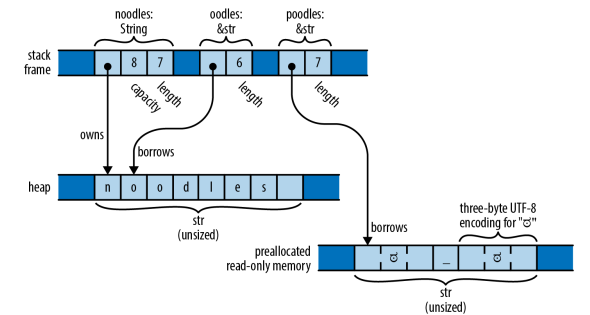
\includegraphics[width=0.8\textwidth]{../img/f3-3.png}
    \caption{\texttt{String, \&str, str}}
    \label{f3-3}
\end{figure}

一个\texttt{String}有一个大小可变的缓冲区来存储UTF-8文本。缓冲区是在堆上分配的,所以他可以按需或按照要求调整缓冲区大小。在这个例子中,\texttt{noodles}是一个拥有8个字节大小的缓冲区的\texttt{String},其中7个字节已经被使用。你可以将\texttt{String}想象为保证内容是有效UTF-8编码的\texttt{Vec<u8>};事实上,\texttt{String}就是这么实现的。

一个\texttt{\&str}(读作“stir”或者“字符串切片”)是一个指向其他值拥有的UTF-8文本的引用:它“借用”了这段文本。在这个例子中,\texttt{oodles}是一个指向\texttt{noodles}所持有的文本中的最后六个字节的\texttt{\&str},因此它表示文本“oodles”。就像其他切片引用一样,\texttt{\&str}是一种胖指针,包括实际数据的地址和长度。你可以将\texttt{\&str}看作一个保证内容为合法的UTF-8编码的\texttt{\&[u8]}。

字符串字面量是一个指向预先分配好内存的文本的\texttt{\&str},实际的文本通常和程序的机器码一起存储到只读的内存区域。在之前的例子中,\texttt{poodles}是一个字符串字面量,指向程序运行时就已经被创建好并且持续到程序退出的7个字节。

一个\texttt{String}或\texttt{\&str}的\texttt{len()}方法返回它的长度。但这个长度是以字节为单位,而不是以字符为单位:
\begin{minted}{Rust}
    assert_eq!("某些卡纳达语字符".len(), 24);
    assert_eq!("某些卡纳达语字符".chars().count(), 8);
\end{minted}

不能修改\texttt{\&str}:
\begin{minted}{Rust}
    let mut s = "hello";
    s[0] = 'c';     // error: `&str`不能被修改,以及其他原因
    s.push('\n');   // error: `&str`没有`push`方法
\end{minted}

要在运行时创建新的字符串,要使用\texttt{String}。

类型\texttt{\&mut str}确实存在,但它并不好用,因为几乎所有对UTF-8的操作都可能改变字节长度,而一个切片不能重新分配它指向的参照物。事实上,\texttt{\&mut str}唯一能做的操作是\texttt{make\_ascii\_uppercase}和\texttt{make\_ascii\_lowercase},这两个操作在原址修改文本,并且只影响单个字节的字符。

\subsection{\texttt{String}}
\texttt{\&str}和\texttt{\&[T]}很像:都是一个指向某些数据的胖指针。\texttt{String}类似于\texttt{Vec<T>},如\hyperref[t3-11]{表3-11}所示。

\begin{table}[htbp]
    \centering
    \caption{\texttt{Vec<T>}和\texttt{String}}的比较
    \label{t3-11}
    \begin{tabular}{p{0.6\textwidth}p{0.15\textwidth}p{0.15\textwidth}}
        \hline
                    & \textbf{\texttt{Vec<T>}} & \textbf{\texttt{String}} \\
        \hline
        自动释放缓冲区 & 是 & 是 \\
        可增长       & 是 & 是 \\
        有\texttt{::new()}和\texttt{::with\_capacity()}类型关联函数 & 是 & 是 \\
        \texttt{.reserve()}和\texttt{.capacity()}方法 & 是 & 是 \\
        \texttt{.push()}和\texttt{.pop()}方法 & 是 & 是 \\
        范围语法\texttt{v[start..stop} & 是,返回\texttt{\&[T]} & 是,返回\texttt{\&str} \\
        自动转换      & \texttt{\&Vec<T>}到\texttt{\&[T]} & \texttt{\&String}到\texttt{\&str} \\
        继承方法      & 从\texttt{\&[T]} & 从\texttt{\&str} \\
    \end{tabular}
\end{table}

类似于\texttt{Vec},每个\texttt{String}都有它自己的在堆上分配的缓冲区,这个缓冲区不和其他任何\texttt{String}共享。当一个\texttt{String}变量离开作用域时,缓冲区会自动释放,除非\texttt{String}被移动了。

有几种方式创建\texttt{String}:
\begin{itemize}
    \item \texttt{.to\_string()}方法把\texttt{\&str}转换为一个\texttt{String},这会拷贝字符串:
    \begin{minted}{Rust}
    let error_message = "too many pets".to_string();
    \end{minted}
    \texttt{.to\_owned()}方法做同样的事,你可能会看到它用同样的方式使用。它也可以用于其他类型,正如我们在\hyperref[ch13]{第13章}讨论的一样。

    \item \texttt{format!()}宏类似于\texttt{println!()},区别在于它返回一个新的\texttt{String}而不是把它打印到标准输出,而且它不会再最后自动加上换行符:
    \begin{minted}{Rust}
    assert_eq!(format!("{}°{:02}′{:02}″N", 24, 5, 23),
               "24°05′23″N".to_string());
    \end{minted}

    \item 字符串的数组、切片、vector都有两个方法\texttt{.concat()}和\texttt{.join(sep)},把多个字符串组合成一个:
    \begin{minted}{Rust}
    let bits = vec!["veni", "vidi", "vici"];
    assert_eq!(bits.concat(), "venividivici");
    assert_eq!(bits.join(", "), "veni, vidi, vici");
    \end{minted}
\end{itemize}

有时你需要选择使用\texttt{\&str}还是\texttt{String}。\hyperref[ch05]{第5章}将详细介绍这个问题。现在你只需要知道\texttt{\&str}可以指向任何字符串的任何切片,不管是字符串字面量(存储在可执行文件中)还是\texttt{String}(在运行时分配和释放)。这意味着当允许调用者传递任何类型的字符串时\texttt{\&str}更适合用作参数的类型。

\subsection{使用字符串}

字符串支持\texttt{==}和\texttt{!=}运算符。只有当两个字符串含有内容和顺序都完全相同的字符时两个字符串才相等(和它们在内存中的位置无关):
\begin{minted}{Rust}
    assert!("ONE".to_lowercase() == "one");
\end{minted}

字符串还支持比较运算符\texttt{<, <=, >, >=},以及很多你可以在在线文档的“\texttt{str}(primitive type)”或“\texttt{std::str}”模块的页面中找到的有用的方法和函数(或者直接跳转到\hyperref[ch17]{第17章})。这里有一些例子:
\begin{minted}{Rust}
    assert!("peanut".contains("nut"));
    assert_eq!("    clean\n".trim(), "clean");

    for word in "veni, vidi, vici".split(", ") {
        assert!(word.starts_with("v"));
    }
\end{minted}

注意,因为Unicode的特性,简单的逐字符比较\emph{并不}总是能给出预期的答案。例如,Rust的字符串\texttt{"th\textbackslash u{e9}"}和\texttt{"the\textbackslash u{301}"}都是有效的\textbf{thé}(法语中表示茶的单词)的Unicode表示。Unicode认为它们它们应该以相同的方式展示和处理,但是Rust把它们当作两个完全不同的字符串。类似的,Rust的比较运算符比如\texttt{<}只是简单的使用基于字符码点值的字典顺序。这种顺序只是偶尔像用户语言和文化中用于文本的排序。我们将在\hyperref[ch17]{第17章}中详细讨论这个问题。

\subsection{其他类似字符串的类型}

Rust保证字符串是有效的UTF-8字符串。有时一个程序可能会需要处理\emph{非}有效的Unicode字符串。这通常发生在Rust程序与其他不强制遵循Unicode的系统交互时。例如,在大多数操作系统中很容易就能创建一个文件名不是有效的Unicode的文件。当Rust遇到这样的文件名时该如何处理?

Rust的方法是为这些场景提供一些类似字符串的类型:
\begin{itemize}
    \item 对于Unicode文本坚持使用\texttt{String}和\texttt{\&str}。
    \item 当处理文件名时,使用\texttt{std::path::PathBuf}和\texttt{\&Path}来代替。
    \item 当处理完全不是UTF-8编码的二进制数据时,使用\texttt{Vec<u8>}和\texttt{\&[u8]}。
    \item 当处理环境变量名称或者命令行参数这些由操作系统提供的内容时,使用\texttt{OsString}和\texttt{\&OsStr}。
    \item 当和以空字符结尾的C库交互时,使用\texttt{std::ffi::CString}和\texttt{\&CStr}。
\end{itemize}

\section{类型别名}

\texttt{type}关键字可以像C++中的\texttt{typedef}一样为已存在的类型声明一个新名字:
\begin{minted}{Rust}
    type Bytes = Vec<u8>;
\end{minted}

我们在这里声明的\texttt{Bytes}就是这种特定类型的\texttt{Vec}:
\begin{minted}{Rust}
    fn decode(data: &Bytes) {
        ...
    }
\end{minted}

\section{基本类型之外}

类型是Rust的一个核心部分。我们将在整本书中继续讨论类型并介绍新的类型。特别是,Rust 的用户定义类型赋予了语言很多自身的风格。有三种用户自定义的类型,我们将分别在三章中介绍它们:\hyperref[ch09]{第9章}介绍结构体,\hyperref[ch10]{第10章}介绍枚举,\hyperref[ch11]{第11章}介绍trait。

函数和闭包有它们自己的类型,这将在\hyperref[ch14]{第14章}中介绍。标准库中的类型将在整本书中介绍。例如,\hyperref[ch16]{第16章}介绍标准集合类型。

不过,这些都还需要等一会。在我们继续之前,是时候了解一下Rust安全规则的核心概念了。

    \chapter{所有权与move}\label{ch04}

在内存管理方面,我们希望编程语言能够具备以下两个特点:
\begin{itemize}
    \item 我们希望内存能在我们想要释放的时候被及时释放。这样我们可以控制程序的内存消耗。
    \item 我们永远不希望使用一个指向已经被释放的对象的指针。这会导致未定义行为,进而导致崩溃和安全漏洞。
\end{itemize}

但这两点看起来似乎是相互矛盾的:释放一个还有指针指向的对象的内存必定会导致悬垂指针。几乎所有的主流编程语言都属于两个阵营之一,取决于它们放弃了哪一点:
\begin{itemize}
    \item “安全优先”的阵营使用垃圾回收来管理内存,自动释放那些没有指针指向的对象。这种做法通过将对象一直保持到没有指针指向来避免悬垂指针。几乎所有的现代语言都落入了这个阵营,包括Python、JavaScript、Ruby、Java、C\#、Haskell。

    但依赖垃圾回收意味着放弃控制对象被回收的精确时间。垃圾收集器通常都令人讨厌,并且理解为什么内存没有如你所料的被释放可能会是一个挑战。

    \item “控制优先”的阵营让你自己负责释放内存。程序的内存消耗完全由你控制,但如何避免悬垂指针成了你最大的问题。C和C++是这个阵营里仅有的主流语言。

    如果你从没犯过错,那说明你很厉害。但证据表明,你最终还是会犯错。指针的错误使用一直都是那些被报导的安全问题的罪魁祸首。
\end{itemize}

Rust旨在同时保证安全和性能,因此这两种阵营都是不可接受的。但如果兼顾两者很简单的话,早就有人做出来了。要想兼顾两者,必须从根本上作出改变。

Rust以一种令人惊讶的方式打破了这个死锁:严格限制程序使用指针的方法。这一章和接下来将专注于解释这些限制和为什么它们能解决问题。你常用的一些程序结构可能也不符合这些规则,你可能需要寻找替代方案。但这些限制的最终效果是给这种混乱带来了足够的秩序,以允许Rust在编译期检查你的程序是否能避免内存安全错误:悬垂指针、两次释放、使用未初始化的内存等。在运行时,你的指针只是简单的地址,就像在C和C++中一样。不同的是你的代码已经被证明是安全的。

这些规则也为Rust实现安全的并发编程奠定了基础。Rust精心设计的线程原语可以让这些保证内存安全的规则也能保证你的代码可以避免数据竞争。Rust程序中的一个bug不可能导致一个线程破坏另一个线程的数据进而导致在不相干的地方出现很难复现的错误。多线程代码中的不确定行为被那些专为它设计的特性——互斥锁、消息通道、原子类型等完全隔离,不会出现在正常的内存访问中。C和C++中的多线程代码臭名昭著,但Rust漂亮地解决了它。

即使有这些限制,你会发现它仍然可以足够灵活地处理几乎所有的任务,而它可以消除内存管理和并发bug的优势将证明你需要改变——你需要对自己的风格进行调整。这是Rust最大的赌注,也是它的核心和成功之处。本书的作者们看好Rust,正是因为我们在C和C++方面有丰富的经验。对我们来说,遵守Rust的规则不费吹灰之力。\footnote{译者注:此处原文:For us, Rust's deal is a no-brainer.}

Rust的规则可能和你在其他编程语言中看到的不同。了解怎么和它们一起工作并利用它们的优势,在我们看来是学习Rust的核心挑战。在这一章中,我们将首先展示相同的潜在问题如何在其他语言中导致问题,以此来深入了解Rust规则背后的逻辑和意图。之后,我们将详细解释Rust的规则、从概念和机制层面探究所有权的含义、如何在各种场景下追踪所有权的变化、以及一些为了提供更大的灵活性而打破这些规则的类型。

\section{所有权}

如果你读过很多C或C++的代码,你可能会看到过有注释说某个类的实例\emph{拥有(own)}某些它指向的其他对象。这一般意味着拥有者可以决定何时释放它拥有的对象:当拥有者被销毁时,它会销毁所有它拥有的对象。

例如,假设你写了如下C++代码:
\begin{minted}{Rust}
    std::string s = "frayed knot";
\end{minted}

字符串\texttt{s}在内存中的表示通常如\hyperref[f4-1]{图4-1}所示:
\begin{figure}
    \centering
    \includegraphics[width=0.8\textwidth]{../img/f4-1.png}
    \caption{一个栈上的C++ \texttt{std::string},指向它在堆上分配的内存}
    \label{f4-1}
\end{figure}

这里,实际上\texttt{std::string}对象本身总是只有3个字长,包括一个指向堆上分配的缓冲区的指针、缓冲区的最大容量(也就是在不重新分配缓冲区的情况下,能存储的最大文本长度),和已经持有的文本的长度。这些都是\texttt{std::string}的私有字段,使用者不能访问。

一个\texttt{std::string}拥有它的缓冲区,当程序销毁string时,它的析构函数会释放缓冲区。以前,一些C++库在多个\texttt{std::string}值之间共享单个缓冲区,使用一个引用计数来决定缓冲区什么时候应该被释放。较新版本的C++标准有效地排除了这种表示,所有现代的C++库都是用上图中的方式。

在这些场景中,人们普遍认为尽管其他代码创建这些被拥有的内存的指针是没问题的,但这些代码有责任确保在所有者决定销毁它拥有的对象之前所有的这种指针都已消失。你可以创建一个指向\texttt{std::string}的缓冲区的指针,但当string被销毁后,你的指针就无效了,你必须自己保证不再使用它。拥有者决定所拥有对象的生命周期,所有其他的对象必须尊重它的决定。

我们在这里使用\texttt{std::string}做为例子展示了C++中的所有权是什么样子的:它只是一个标准库普遍遵守的规范。然而即使语言鼓励你也遵守相似的实践,但如何设计你自己的类型最终还是取决于你。

但在Rust中,所有权的概念被内建在语言之中,并且通过编译期检查确保强制执行。每个值都只有一个决定它生命周期的所有者。当所有者被释放——Rust中的术语叫\emph{dropped}——它拥有的值也会被dropped。这些规则的目的是让你可以通过检查代码很容易的查明某个值的生命周期,并给你系统语言应有的控制生命周期的能力。

一个变量拥有它的值。当控制流离开了变量声明的语法块,变量会被drop,因此它的值也会随之一起drop。例如:
\begin{minted}{Rust}
    fn print_padovan() {
        let mut padovan = vec![1,1,1];  // 在这里分配
        for i in 3..10 {
            let next = padovan[i-3] + padovan[i-2];
            padovan.push(next);
        }
        println!("P(1..10) = {:?}", padovan);
    }
\end{minted}

变量\texttt{padovan}的类型是\texttt{Vec<i32>},一个32位整数的vector。在内存中,\texttt{padovan}看起来将类似于\hyperref[f4-2]{图4-2}。

\begin{figure}[htbp]
    \centering
    \includegraphics[width=0.8\textwidth]{../img/f4-2.png}
    \caption{栈上的\texttt{Vec<i32>},指向它在堆上的缓冲区}
    \label{f4-2}
\end{figure}

这和我们之前展示的C++的\texttt{std::string}非常像,除了缓冲区里的元素是32位整数,而不是字符。注意存储\texttt{padovan}的指针、容量和长度的字都在\texttt{print\_padovan}函数的栈帧中,只有vector的缓冲区是在堆上分配的。

和之前展示的string \texttt{s}一样,vector拥有它用来存储元素的缓冲区。当变量\texttt{padovan}在函数结尾处离开作用域时,程序会drop这个vector。因为vector拥有它的缓冲区,缓冲区也会随之drop。

Rust的\texttt{Box}类型是另一个所有权的例子。\texttt{Box<T>}是一个指针,指向一个存储在堆上的类型\texttt{T}的值,调用\texttt{Box::new(v)}会在堆上分配一些空间,把值\texttt{v}移动进去,然后返回一个\texttt{Box}指向堆上的空间。因为一个\texttt{Box}拥有它所指向的空间,当\texttt{Box}被drop的时候,堆上的空间也会被释放。

例如,你可以像这样在堆上分配一个元组:
\begin{minted}{Rust}
    {
        let point = Box::new((0.625, 0.5));     // point在这里分配
        let label = format!("{:?}", point);     // label在这里分配
        assert_eq!(label, "(0.625, 0.5)");
    }                                           // point和label都在这里drop
\end{minted}

当程序调用\texttt{Box::new}时,它会在堆上为一个由两个\texttt{f64}值组成的元组分配空间,把它的参数\texttt{(0.625, 0.5)}移动进去,然后返回一个指向它的指针。当控制流到达\texttt{assert\_eq!}的调用时,栈帧如\hyperref[f4-3]{图4-3}所示。

\begin{figure}[htbp]
    \centering
    \includegraphics[width=0.8\textwidth]{../img/f4-3.png}
    \caption{两个本地变量,每个都拥有堆上的一块内存}
    \label{f4-3}
\end{figure}

栈帧本身存储了变量\texttt{point}和\texttt{label},每一个变量都指向自己拥有的堆上的内存。当它们被drop时,它们拥有的内存也随之释放。

与变量拥有它们的值类似,结构体拥有它们的字段,元组、数组、vector拥有它们的元素。

\begin{minted}{Rust}
    struct Person { name: String, birth: i32 }
    let mut composers = Vec::new();
    composers.push(Person { name: "Palestrina".to_string(),
                            birth: 1525 });
    composers.push(Person { name: "Dowland".to_string(),
                            birth: 1563 });
    composers.push(Person { name: "Lully".to_string(),
                            birth: 1632 });
    for composer in &composers {
        println!("{}, born {}", composer.name, composer.birth);
    }
\end{minted}

这里,\texttt{composers}是一个\texttt{Vec<Person>}:一个结构体的vector,每个结构体有一个字符串和数字。在内存中,\texttt{composers}的最终结果如\hyperref[f4-4]{图4-4}所示。

\begin{figure}[htbp]
    \centering
    \includegraphics[width=0.8\textwidth]{../img/f4-4.png}
    \caption{一个更复杂的所有权树}
    \label{f4-4}
\end{figure}

这里有很多的所有权关系,但每一个都很直观:\texttt{composers}拥有一个vector,vector拥有它的元素,每一个元素是一个\texttt{Person}结构体;每个结构体拥有它的字段;其中的字符串字段拥有它的文本。当控制流离开了\texttt{composers}声明的作用域,程序会drop它的值,同时drop它拥有的所有内容。如果这里还有其他类型的集合,例如\texttt{HashMap}、\texttt{BTreeSet},那么过程也是一样的。

到这里,让我们退后一步并思考我们到目前为止展示的所有权关系。每个值都只有一个所有者,这样很容易决定什么时候drop这个值。但单个值可能拥有很多其他值:例如,vector \texttt{composers}拥有它的所有元素。这些元素也可能反过来拥有其他值:\texttt{composers}的每个元素拥有一个字符串,字符串又拥有它的文本。

所有者和它们拥有的值组成了\emph{树}:值的拥有者是它的父结点,值拥有的值是它的孩子结点。每棵树的根结点是一个变量;当这个变量离开作用域时,整个树都会随之销毁。我们可以在\texttt{composers}的图中看到这样一棵所有权的树:它不是搜索树数据结构意义上的“树”、也不是DOM元素组成的HTML文档树。相反,我们有一个由混合类型构建的树,Rust的单一所有者规则禁止任何可能使布局变得比树更复杂的连接操作。Rust程序中的每个值都是树中的一个结点,树的根就是变量。

Rust程序通常完全不需要像C和C++程序中使用\texttt{free}和\texttt{delete}一样显式drop值。Rust\\
中drop值的方式是将它从所有权树移除:当离开作用域时、或者从vector中删除元素时、或者类似的情况。这时,Rust保证值会和它拥有的所有值一起被drop掉。

在某种意义上,Rust不如其他语言强大:每个其他的编程语言都允许你在对象之间构建任意的关系图,这些对象以你认为合适的方式互相指向。但正因为Rust不够强大,所以它才可以对你的程序进行更强大的分析。Rust的安全保证可以实现的原因就是你的代码中可能出现的所有权关系更加容易处理。这是我们之前提到的Rust的“激进赌注”的一部分:Rust声称,在实践中,解决问题时通常有足够的灵活性来保证至少有一些完美的解决方案可以在语言强加的限制范围内实现。

也就是说,我们到目前为止解释的所有权的概念太过死板以至于很难使用。Rust在以下几个方面扩展了这个简单的想法:
\begin{itemize}
    \item 你可以将值从一个所有者移动到另一个所有者。这允许你构建、更改、拆除所有权树。
    \item 很简单的类型例如整数、浮点数和字符被所有权规则排除在外。它们被称为\texttt{Copy}类型。
    \item 标准库提供了引用计数的指针类型\texttt{Rc}和\texttt{Arc},它们允许值在一定的限制下可以有多个所有者。
    \item 你可以“借用一个值的引用”,引用是生命周期受限的非占有的指针。
\end{itemize}

这些策略中的每一条都改善了所有权模型的灵活性,同时仍然坚持Rust的承诺。我们将依次介绍它们,引用将在下一章介绍。

\section{move}
在Rust里对大多数类型来说,赋值给变量、把值传给函数、或者从函数返回值并不会拷贝这个值:它们只会\emph{move}它。源对象放弃了值的所有权,把所有权转移给了目的对象,同时源对象变为未初始化的状态;此时目的对象控制值的生命周期。Rust程序一次一个值、一次move一个地构建和拆除复杂的结构。

你可能会很惊讶Rust改变了这些基础操作的含义。确实赋值操作很早之前就已经有了明确的含义。然而,如果你仔细观察过不同的语言是怎么处理赋值操作的,你就会发现不同语言的处理方式有很大差别。这种差别也让我们能更容易的看出Rust的选择的含义和结果。

考虑下面的Python代码:
\begin{minted}{python}
    s = ['udon', 'ramen', 'soba']
    t = s
    u = s
\end{minted}

每一个Python对象都有一个引用计数,用来追踪当前有多少个值指向它。因此在对\texttt{s}赋值以后,程序的状态如\hyperref[f4-5]{图4-5}所示(注意有一些内容被省略了)。

\begin{figure}[htbp]
    \centering
    \includegraphics[width=0.9\textwidth]{../img/f4-5.png}
    \caption{Python如何在内存中表示一个字符串的列表}
    \label{f4-5}
\end{figure}

因为只有\texttt{s}指向列表,所以列表的引用计数是1;因为列表是唯一指向那些字符串的对象,所以每个字符串的引用计数也是1。

当程序执行到\texttt{t}和\texttt{u}的赋值时会发生什么?Python把赋值操作简单实现为让目标变量也指向源变量指向的对象,然后增加对象的引用计数。因此,这段程序的最终状态如\hyperref[f4-6]{图4-6}所示:
\begin{figure}[htbp]
    \centering
    \includegraphics[width=0.8\textwidth]{../img/f4-6.png}
    \caption{在Python里把\texttt{s}赋值给\texttt{t}和\texttt{u}的结果}
    \label{f4-6}
\end{figure}

Python拷贝了\texttt{s}的指针,并赋给了\texttt{t}和\texttt{u},然后把列表的引用计数更新为3。Python中的赋值开销很低,但因为它创建了新的指向对象的引用,我们必须维护引用计数来知道我们什么时候可以释放值。

现在考虑下面类似的C++代码:
\begin{minted}{C++}
    using namespace std;
    vector<string> s = { "udon", "ramen", "soba" };
    vector<string> t = s;
    vector<string> u = s;
\end{minted}

一开始\texttt{s}的值在内存中如\hyperref[f4-7]{图4-7}所示。

\begin{figure}[htbp]
    \centering
    \includegraphics[width=0.8\textwidth]{../img/f4-7.png}
    \caption{C++里一个字符串的vector在内存中的表示}
    \label{f4-7}
\end{figure}

当把\texttt{s}赋值给\texttt{t}和\texttt{u}时会发生什么呢?在C++里赋值一个\texttt{std::vector}会产生一份这个vector的拷贝;\texttt{std::string}的行为类似。因此当程序到达末尾时,它实际上有3个vector和\\
9个字符串(\hyperref[f4-8]{图4-8})。

\begin{figure}[htbp]
    \centering
    \includegraphics[width=0.8\textwidth]{../img/f4-8.png}
    \caption{在C++里把\texttt{s}赋值给\texttt{t}和\texttt{u}的结果}
    \label{f4-8}
\end{figure}

根据值的不同,C++里的赋值可能会消耗任意数量的内存和处理器时间。然而,它的优势是,程序可以很容易的决定何时释放这些内存:当变量离开作用域时,所有这里分配的内存都会被自动释放。

某种意义上,C++和Python选择了相反的策略:Python里赋值操作开销很小,但引用计数(通用一点的说法,垃圾回收)开销很大。C++保持了内存的所有权都很清楚,但赋值时会执行对象的深拷贝导致开销很大。C++程序员通常不太热衷于这种选择:深拷贝可能开销很大,通常会有更好的替代方法。

那么Rust中的类似程序会怎么做呢?代码如下:
\begin{minted}{Rust}
    let s = vec!["udon".to_string(), "ramen".to_string, "soba".to_string()];
    let t = s;
    let u = s;
\end{minted}

类似于C和C++,Rust把字符串字面量例如\texttt{"udon"}存储在只读内存中,因此,为了更清楚地与C++和Python的例子进行对比,我们调用了\texttt{to\_string}来获得在堆上分配的\texttt{String}值。

在\texttt{s}的初始化之后,因为Rust和C++有相似的vector和string表示,所以看起来和C++中的情况很像(\hyperref[f4-9]{图4-9})。

\begin{figure}[htbp]
    \centering
    \includegraphics[width=0.8\textwidth]{../img/f4-9.png}
    \caption{Rust中一个字符串的vector在内存中的表示}
    \label{f4-9}
\end{figure}

但回想一下,Rust里大多数类型的赋值操作都是把值从源对象\emph{移动}到目的对象,然后源对象变为未初始化的状态。因此\texttt{t}初始化完之后,程序的内存状态如\hyperref[f4-10]{图4-10}所示。

\begin{figure}[htbp]
    \centering
    \includegraphics[width=0.8\textwidth]{../img/f4-10.png}
    \caption{Rust里把\texttt{s}赋值给\texttt{t}之后的结果}
    \label{f4-10}
\end{figure}

这里发生了什么?赋值语句\texttt{let t = s;}把vector的三个字段从\texttt{s}移动到了\texttt{t};现在\texttt{t}拥有了这个vector。vector的元素则仍待在原来的位置,string的位置也没有发生变化。每一个值都只有一个所有者,尽管所有者已经变了。不需要调整引用计数,并且编译器现在把\texttt{s}视作未初始化的状态。

因此当我们到达\texttt{let u = s;}时会发生什么呢?这将会把\texttt{s}赋值给\texttt{u}。Rust禁止使用未初始化的值,所以编译器会报如下错误:
\begin{minted}{text}
    error[E0382]: use of moved value: `s`
      |
    7 |     let s = vec!["udon".to_string(), "ramen".to_string(), "soba".to_string()];
      |         - move occurs because `s` has type `Vec<String>`,
      |           which does not implement the `Copy` trait
    8 |     let t = s;
      |             - value moved here
    9 |     let u = s;
      |             ^ value used after move
\end{minted}

考虑Rust在这里使用move的结果。类似于Python,赋值操作开销很小,程序简单地把vector的三个字长的头部从一个点移动到了另一个点。但和C++类似,所有权总是很清晰:程序不需要引用计数或者垃圾回收来判断什么时候释放vector的元素和string的内容。

而为此付出的代价是如果赋值时想要的是拷贝操作那么必须显式写出。如果你想要最后和C++程序一样的状态,也就是每个变量都有独立的拷贝,那么必须调用vector的\texttt{clone}方法,它会对vector和它的元素执行深拷贝:
\begin{minted}{Rust}
    let s = vec!["udon".to_string(), "ramen".to_string(), "soba".to_string()];
    let t = s.clone();
    let u = s.clone();
\end{minted}

你也可以通过Rust的引用计数指针类型复现Python代码的行为,我们将在\hyperref[rc]{Rc和Arc:共享所有权}这一节中简要介绍这一点。

\subsection{更多move的操作}

在我们上面展示的初始化例子中,都是在使用\texttt{let}语句引入变量的同时把值赋给它们。赋值给一个变量将与此有细微的不同,如果你把值移动进一个已经被初始化的变量,Rust会drop变量之前的值。例如:
\begin{minted}{Rust}
    let mut s = "Govinda".to_string();
    s = "Siddhartha".to_string();   // 值"Govinda"在这里drop
\end{minted}

在这段代码中,当程序把\texttt{"Siddhartha"}赋值给\texttt{s}时,它之前的值\texttt{"Govinda"}首先被drop掉。但考虑下面的代码:
\begin{minted}{Rust}
    let mut s = "Govinda".to_string();
    let t = s;
    s = "Siddhartha".to_string();   // 这里不会drop任何内容
\end{minted}

这一次,\texttt{t}拿走了\texttt{s}中原本的字符串的所有权,因此当我们给\texttt{s}赋值时,它是未初始化的。在这种场景下,不会发生drop。

我们在这里使用初始化和赋值的例子是因为它们足够简单,但Rust在几乎所有场景下都使用move。向函数传参会把所有权移动给函数的参数;从函数返回值会把所有权移动给调用者;创建一个元组会把值移动给元组,等等。

你现在可能对我们之前章节给出的例子中到底发生了什么有了更深入的理解。例如,当我们构建作曲家的vector时,我们写了:
\begin{minted}{Rust}
    struct Person { name: String, birth: i32 }

    let mut composers = Vec::new();
    composers.push(Person { name: "Palestrina".to_string(), 
                            birth: 1525 });
\end{minted}

这段代码展示了除了初始化和赋值之外,move发生的几个场景:
\begin{flushleft}
    \emph{从函数返回值}
\end{flushleft}

\hangparagraph{调用\texttt{Vec::new()}会创建一个新的vector并返回,返回的并不是指向vector的指针,而是vector本身:它的所有权从\texttt{Vec::new}移动到了变量\texttt{composers}。类似的,\texttt{to\_string}调用返回了一个新的\texttt{String}实例。}

\begin{flushleft}
    \emph{构造新的值}
\end{flushleft}

\hangparagraph{新的\texttt{Person}结构体的\texttt{name}字段被\texttt{to\_string}的返回值初始化。结构体获得了这个字符串的所有权。}

\begin{flushleft}
    \emph{向函数传递值}
\end{flushleft}

\hangparagraph{整个\texttt{Person}结构体,而不是指向它的指针,被传递给vector的\texttt{push}方法,这个方法将值移动到了结构体的尾部。vector获得了\texttt{Person}的所有权,因此也变成了name \texttt{String}的间接所有者。}

像这样移动值可能听起来并不是很高效,但有两件事需要记住。第一,move只作用于恰当的值,而不作用于它们拥有的堆存储。对于vector和string来说,\emph{恰当的值}是它们三个字长的头部,潜在的很多元素的数组和文本缓冲区仍然停留在堆中原本的位置。第二,Rust编译器的代码生成部分擅长“看穿”所有这些move;在实践中,机器码通常会直接把值存储到它最终的位置。

\subsection{move和控制流}
之前的例子中的控制流都很简单,move会如何影响更复杂的代码呢?通用的原则是,如果一个变量的值被移动走并且从此之后没有再被赋予一个新的值,那么它被认为是未初始化的。例如,如果一个变量在\texttt{if}表达式的条件判断之后还是有值的,那我们在两个分支中都可以使用它:
\begin{minted}{Rust}
    let x = vec![10, 20, 30];
    if c {
        f(x);   // ... 在这里移动x的值是ok的
    } else {
        g(x);   // ... 在这里移动x的值也是ok的
    }
    h(x);   // 错误:如何任何一个分支使用了x,那么x在此处将是未初始化的
\end{minted}

出于类似的原因,在循环里移动一个变量的值是禁止的:
\begin{minted}{Rust}
    let x = vec![10, 20, 30];
    while f() {
        g(x);   // 错误:x会在第一次迭代时被移动
                // 第二次迭代时就是未初始化状态 
    }
\end{minted}

也就是说,我们需要在每次迭代里都重新赋予它一个新值:
\begin{minted}{Rust}
    let mut x = vec![10, 20, 30];
    while f() {
        g(x);       // 移动x的值
        x = h();    // 给x一个新值
    }
\end{minted}

\subsection{move和索引}

我们已经提到过move会将源对象设置为未初始化状态,目的对象会获得值的所有权。但并不是每一种值的所有者都可以设置为未初始化状态。例如,考虑下面的代码:
\begin{minted}{Rust}
    // 创建一个string的vector:"101", "102", ... "105"
    let mut v = Vec::new();
    for i in 101 .. 106 {
        v.push(i.to_string());
    }

    // 从vector中取出随机的元素
    let third = v[2];   // 错误:不能移动Vec的索引
    let fifth = v[4];   // 这里也是一样
\end{minted}

如果想让这段代码工作,Rust需要记住这个vector的第3和第5个元素变成了未初始化状态,然后一直追踪这些信息直到这个vector被drop。在一般情况下,vector需要携带额外的信息来指示哪些元素还可用,哪些变为了未初始化。显然这不是一门系统编程语言应该有的行为;一个vector应该只是一个vector。事实上,Rust会报错拒绝上面的代码:
\begin{minted}{text}
    error[E0507]: cannot move out of index of `Vec<String>`
       |
    14 |     let third = v[2];
       |                 ^^^^
       |                 |
       |                 move occurs because value has type `String`,
       |                 which does not implement the `Copy` trait
       |                 help: consider borrowing here: `&v[2]`
\end{minted}

移动到\texttt{fifth}的语句也会报类似的错误。在这些错误信息中,Rust建议使用引用,这样就可以在不移动的情况下访问元素。这通常是你想要的。但如果我们真的想从vector中移出一个元素呢?你需要找到一些不违反类型限制的方法来做这件事。这里有三种方法:
\begin{minted}{Rust}
    // 创建一个string的vector:"101", "102", ... "105"
    let mut v = Vec::new();
    for i in 101 .. 106 {
        v.push(i.to_string());
    }

    // 1. 弹出vector尾部的元素
    let fifth = v.pop().expect("vector empty!");
    assert_eq!(fifth, "105");

    // 2. 移出给定位置的元素,并把最后一个元素移动过来:
    let second = v.swap_remove(1);
    assert_eq!(second, "102");

    // 3. 用另一个值和我们想移出的值交换
    let third = std::mem::replace(&mut v[2], "substitute".to_string());
    assert_eq!(third, "103");

    // 让我们看看vector中还剩下什么。
    assert_eq!(v, vec!["101", "104", "substitute"]);
\end{minted}

这三种方法都从vector中移出一个元素,但仍然保证vector处于没有空隙的状态,可能长度还会变小。

像\texttt{Vec}这样的集合类型也提供方法通过循环消费它们的所有元素:
\begin{minted}{Rust}
    let v = vec!["liberté".to_string(),
                 "égalité".to_string(),
                 "fraternité".to_string()];
    for mut s in v {
        s.push('!');
        println!("{}", s);
    }
\end{minted}

当直接把vector传给循环时,例如\texttt{for ... in v},这会把\texttt{v}中的所有元素\emph{移出}vector,然后\texttt{v}变为未初始化。\texttt{for}循环内部的机制会获取vector的所有权,然后把它分解为若干元素。每一次迭代时,循环都会把一个元素移动到变量\texttt{s}。因为\texttt{s}现在拥有这个字符串,所以我们可以在循环里修改它,然后再打印。因为vector本身不再对代码可见,所以在循环的过程中当它部分为空时没有任何东西可以观测到它。

如果你确实发现你需要从所有者中移出一个编译器无法追踪的值,你可以考虑将所有者的类型改为可以动态追踪是否有值的类型。例如,这里有一个之前示例的变体:
\begin{minted}{Rust}
    struct Person { name: Option<String>, birth: i32 }

    let mut composers = Vec::new();
    composers.push(Person { name: Some("Palestrina".to_string()),
                            birth: 1525 });
\end{minted}

你不能这样做:
\begin{minted}{Rust}
    let first_name = composers[0].name;
\end{minted}

这只会和犯和之前一样的“不能移出索引”的错误。但因为你把\texttt{name}字段的类型从\texttt{String}改为了\texttt{Option<String>},这意味着\texttt{None}是这个字段的一个合法的取值,因此下面的代码可以生效:
\begin{minted}{Rust}
    let first_name = std::mem::replace(&mut composers[0].name, None);
    assert_eq!(first_name, Some("Palestrina".to_string()));
    assert_eq!(composers[0].name, None);
\end{minted}

\texttt{replace}调用移出了\texttt{composers[0].name}的值,留下了一个\texttt{None},并把原本的值的所有权传递给了调用者。事实上,这种使用\texttt{Option}的方法非常普遍,所以这个类型提供了一个\texttt{take}方法来实现这个特殊的用途。你可以使用下面的代码更清晰地完成上述操作:
\begin{minted}{Rust}
    let first_name = composers[0].name.take();
\end{minted}
这里的\texttt{take}调用和之前的\texttt{replace}调用有相同的效果。

\section{Copy类型:move的例外}\label{copy}
到目前为止我们的例子涉及vector、string、和其他可能潜在地使用大量内存并且拷贝开销很大的类型。move保证了这些类型的所有权的明晰、也保证了赋值的开销很小。但对于简单类型例如整数或字符,这种谨慎的处理方式事实上并不是必须的。

让我们比较一下赋值一个\texttt{String}和赋值一个\texttt{i32}值时内存中会发生什么:
\begin{minted}{Rust}
    let string1 = "somnambulance".to_string();
    let string2 = string1;

    let num1: i32 = 36;
    let num2 = num1;
\end{minted}

运行完这段代码后,内存布局如\hyperref[f4-11]{图4-11}所示。
\begin{figure}[htbp]
    \centering
    \includegraphics[width=0.9\textwidth]{../img/f4-11.png}
    \caption{赋值\texttt{String}会移动它,而赋值\texttt{i32}会拷贝它}
    \label{f4-11}
\end{figure}

类似于之前的vector,赋值会把\texttt{string1}\emph{移动}到\texttt{string2},这样我们就不会得到两个负责释放同一个缓冲区的字符串。然而,\texttt{num1}和\texttt{num2}的情况与此不同。\texttt{i32}只是在内存中的一种位模式,它并不拥有任何堆上的资源、也不依赖任何它本身所占的字节之外的东西。此时如果我们把它的位都移动给\texttt{num2},我们就得到了一个和\texttt{num1}完全互相独立的拷贝。

移动一个值会导致源对象变为未初始化。但是尽管把\texttt{string1}视为无值是一个基本的目的,但如果对\texttt{num1}也这么做是毫无意义的,继续使用\texttt{num1}不会导致任何危害。move的优势在这里并不适用,反而变得不够便捷。

之前我们谨慎的说过\emph{大多数}类型会被移动,现在我们来到了例外的情况,也就是Rust称之为\texttt{Copy type}的类型。赋予一个\texttt{Copy}类型的值会拷贝它,而不是移动它。源对象仍然保持初始化状态和可用性,它的值不会发生改变。向函数和构造器传递\texttt{Copy}类型也类似。

标准的\texttt{Copy}类型包括所有的机器整数和浮点数类型、\texttt{char}和\texttt{bool}类型,以及少数其他类型。\texttt{Copy}类型的元组或者固定大小的数组也是\texttt{Copy}类型。

只有简单的逐位拷贝的类型才可以是\texttt{Copy}类型。正如我们解释过的,\texttt{String}不是\texttt{Copy}类型,因为它拥有一个在堆上分配的缓冲区;与此类似,\texttt{Box<T>}也不是\texttt{Copy}类型,它拥有一个堆上分配的对象;代表操作系统中文件句柄的\texttt{File}类型,也不是\texttt{Copy}类型,赋值这样一个值意味着向操作系统请求另一个文件句柄。类似的,表示一个互斥锁的\texttt{MutexGuard}类型,也不是\texttt{Copy}类型,拷贝这个类型没有任何意义,因为在一个时间点只有一个线程可以持有锁。

根据经验,任何在drop时要做一些特殊事情的类型不可能是\texttt{Copy}类型:一个\texttt{Vec}需要释放它的内存,一个\texttt{File}需要关闭它的文件句柄,一个\texttt{MutexGuard}需要释放它的锁,等等。对这些类型逐位拷贝会导致搞不清它们中的哪一个要负责释放原始的资源。

自定义的类型呢?默认情况下,\texttt{struct}和\texttt{enum}不是\texttt{Copy}类型:
\begin{minted}{Rust}
    struct Label { number: u32 }
    fn print(l: Label) { println!("STAMP: {}", l.number); }

    let l = Label { number: 3 };
    print(l);
    println!("My label number is: {}", l.number);
\end{minted}

这不能通过编译,Rust会报错:
\begin{minted}{text}
    error: borrow of moved value: `l`
       |
    10 |     let l = Label { number: 3 };
       |         - move occurs because `l` has type `main::Label`,
       |           which does not implement the `Copy` trait
    11 |     print(l);
       |           - value moved here
    12 |     println!("My label number is: {}", l.number);
       |                                        ^^^^^^^^
       |                  value borrowed here after move
\end{minted}

因为\texttt{Label}不是\texttt{Copy}类型,将它传递给\texttt{print}会把值的所有权移动给\texttt{print}函数的参数,在函数返回时会drop掉值。但这非常愚蠢,一个\texttt{Label}只是一个\texttt{u32}套壳。没有理由将\texttt{l}传递给\texttt{print}时应该移动值。

但用户自定义类型只是默认不是\texttt{Copy}类型。如果你的结构体的所有字段都是\texttt{Copy}类型,那么你可以通过在定义上方加上属性\texttt{\#[derive(Copy, Clone)]}来把它变为\texttt{Copy}类型,像这样:
\begin{minted}{Rust}
    #[derive(Copy, Clone)]
    struct Label { number: u32 }
\end{minted}

这样修改之后,上面的代码就可以通过编译了。然而,如果我们用不是\texttt{Copy}类型的字段来修改这个类型的话,也不能通过编译。假设我们要编译下面的代码:
\begin{minted}{Rust}
    #[derive(Copy, Clone)]
    struct StringLabel { name: String }
\end{minted}

它会报这样的错误:
\begin{minted}{text}
    error[E0204]: the trait `Copy` may not be implemented for this type
     --> ownership_string_label.rs:7:10
      |
    7 | #[derive(Copy, Clone)]
      |          ^^^^
    8 | struct StringLabel { name: String }
      |                      ------------ this field does not implement `Copy`
\end{minted}

为什么不默认把用户自定义类型设置为\texttt{Copy}类型?一个类型是否是\texttt{Copy}类型对接下来的代码如何使用它有巨大的影响:\texttt{Copy}类型更加的灵活,因为赋值和相关的操作不会导致源对象变得未初始化。但对于类型的实现者来说,恰恰相反:\texttt{Copy}类型所能包含的类型十分有限,而非\texttt{Copy}类型可以使用堆上的内存并且拥有自己的资源。因此将一个类型标记为\texttt{Copy}代表着实现者的一个承诺:如果之后它必须要修改为非\texttt{Copy}类型,很多使用它的代码都需要修改。

虽然C++允许你重载赋值运算符和自定义拷贝和移动构造函数,但Rust不允许这种自定义。在Rust里,所有的移动都是逐字节的浅拷贝,同时把源对象设置为未初始化。拷贝与此类似,除了源对象仍然是初始化过的状态。这确实意味着C++类可以提供Rust类所不能提供的方便接口:看起来普通的代码会隐式的调整引用计数、推迟开销很大的拷贝操作、或者使用其它复杂的实现技巧。

但C++中的这种灵活性会导致基本操作例如赋值、传参、返回值变得不可预料。例如,这一章之前的部分我们展示过在C++里把一个变量赋给另一个可能会需要任意数量的内存和处理器时间。Rust的原则之一就是开销对程序员来说必须是明显的。基本的操作必须保持简单。潜在的开销很大的操作必须是显式的,例如在更早的例子中调用\texttt{clone}来获取vector和它包含的string的深拷贝。

在这一节中,我们谈到了术语\texttt{Copy}和\texttt{Clone},模糊地将它们视作类型具有的特征。事实上,它们是\texttt{trait}的示例,它是Rust的一个开发的工具,你可以通过它根据类型能做什么对类型进行分类。我们将在\hyperref[ch11]{第11章}中讨论一般性的trait,在\hyperref[ch13]{第13章}中专门讨论\texttt{Copy}和\texttt{Clone}。

\section{Rc和Arc:共享所有权}\label{rc}

尽管典型的Rust代码中几乎所有的值都只有一个所有者,但在一些情况下,很难让每个值的所有者都有你想要的生命周期,这时你可能会希望值一直保持有效,直到每一个所有者都使用完它。对于这种情况,Rust提供了引用计数类型\texttt{Rc}和\texttt{Arc}。正如你对Rust的期待一样,它们是安全的:你不可能忘记调整引用计数、创建其它指向它的指针、或者出现其他使用C++的引用计数指针类型时可能出现的问题。

\texttt{Rc}和\texttt{Arc}类型非常相似,它们唯一的不同之处在于\texttt{Arc}可以直接安全地在线程之间共享——名称\texttt{Arc}是\emph{原子引用计数}的缩写——\texttt{Rc}则使用更快一些的非线程安全代码来更新引用计数。如果你不需要在线程之间共享指针,那就没有必要承担\texttt{Arc}的性能损失,所以你应该使用\texttt{Rc};Rust会阻止你无意间在线程之间传递\texttt{Rc}。这两种类型在其他方面都是等价的,因此在本节的剩余部分,我们将只讨论\texttt{Rc}。

之前我们曾经展示过Python使用引用计数来管理值的生存周期。你可以使用\texttt{Rc}来在Rust中实现相似的效果。考虑下面的代码:
\begin{minted}{Rust}
    use std::rc::Rc;

    // Rust可以推断出所有这些类型,写出来是为了更清楚
    let s: Rc<String> = Rc::new("shirataki".to_string());
    let t: Rc<String> = s.clone();
    let u: Rc<String> = s.clone();
\end{minted}

对于任意类型\texttt{T},一个\texttt{Rc<T>}值是一个指向在堆上分配的\texttt{T}类型值的指针,同时还附有一个引用计数。克隆一个\texttt{Rc<T>}类型的值并不意味着拷贝\texttt{T},它只是简单的创建另一个指向它的指针,并且递增引用计数。因此上面的代码会产生如\hyperref[f4-12]{图4-12}所示的内存布局:

\begin{figure}[htbp]
    \centering
    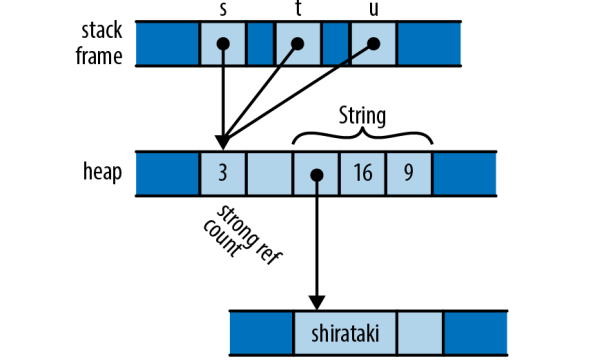
\includegraphics[width=0.8\textwidth]{../img/f4-12.png}
    \caption{一个有三个引用的引用计数字符串}
    \label{f4-12}
\end{figure}

这三个\texttt{Rc<String>}指针都指向内存中的同一块内存,这块内存里存储了一个引用计数和一个\texttt{String}。通常的所有权规也适用于\texttt{Rc}指针,当最后一个\texttt{Rc}指针drop时,Rust会同时drop掉\texttt{String}。

你可以直接对\texttt{Rc<String>}使用任何\texttt{String}的方法:
\begin{minted}{Rust}
    assert!(s.contains("shira"));
    assert_eq!(t.find("taki"), Some(5));
    println!("{} are quite chewy, almost bouncy, but lack flavor", u);
\end{minted}

一个\texttt{Rc}指针拥有的值是不可变的。假设你尝试在字符串的结尾添加文本:
\begin{minted}{Rust}
    s.push_str(" noodles");
\end{minted}

Rust将会报错:
\begin{minted}{text}
    error: cannot borrow data in an `Rc` as mutable
      --> ownership/ownership_rc_mutability.rs:13:5
       |
    13 |     s.push_str(" noodles");
       |     ^ cannot borrow as mutable
       |
\end{minted}

Rust的内存和线程安全保证依赖于没有值既是共享的又是可变的。Rust假设\texttt{Rc}指针指向的值要被共享,因此它必须是不可变的。我们将在\hyperref[ch05]{第5章}解释为什么限制要这么严格。

 使用引用计数来管理内存的一个已知问题就是,如果两个引用计数的值互相指向彼此,那么每一个都会导致对方的引用计数不可能降到0,因此值永远不会被释放(\hyperref[f4-13]{图4-13})。

 \begin{figure}[htbp]
    \centering
    \includegraphics[width=0.8\textwidth]{../img/f4-13.png}
    \caption{一个引用计数循环,这些对象永远不会被释放}
    \label{f4-13}
 \end{figure}

在Rust中出现这种泄漏是可能的,但这种情况非常少见。要想创建这样一个循环,你必须让旧值指向新值,这也意味着旧值要是可变的。因为\texttt{Rc}指针指向的值不可变,所以通常是不能创建这样的循环的。然而,Rust确实提供了一些方法创建部分可变的值的方法;这被称为\emph{内部可变性},我们将在\hyperref[intermut]{内部可变性}一节中介绍。如果你将那些技术和\texttt{Rc}指针结合使用,那么你确实能创建出一个循环,然后造成内存泄漏。

你可以使用\emph{弱指针}\texttt{std::rc::Weak}来避免使用\texttt{Rc}指针创建循环的情况。然而,我们不会在本书中介绍这些,你可以查看标准库的文档获取详情。

move和引用计数指针是两种缓解所有权树过于死板的方法。在下一章中,我们将看到第三种方法:借用值的引用。一旦你对所有权和借用都感到很舒服,那你就已经跨过了Rust的学习曲线中最陡峭的部分,而且已经准备好接受Rust独特的优势。

    \chapter{引用}\label{ch05}

\emph{Libraries cannot provide new inabilities.}

\begin{flushright}
——Mark Miller
\end{flushright}

我们至今为止见过的所有指针类型——简单的\texttt{Box<T>}堆指针、\texttt{String}和\texttt{Vec}内部的指针都拥有值:当所有者被drop时,指针指向的值也会随之消失。Rust还有非拥有指针类型,称为\emph{引用},引用对指向的值的生命周期没有影响。

事实上,正相反,引用绝不应该比它们指向的值活的更长。你必须在你的代码中明确表明引用的寿命比它指向的值更短。为了强调这一点,Rust将创建某个值的引用称为\emph{借用(borrow)}值:最终必须把借走的还给所有者。

如果你在读到“你必须在你的代码中明确表明”时感到一阵怀疑,那说明你很优秀。引用自身并没有什么特殊的——本质上,它们只是地址。但保证它们安全的规则是Rust独有的,你以前不可能看到过类似的。尽管这些规则是Rust里最难掌握的部分,但它们能防止的经典的、日常的bug的范围之广令人惊讶,它们对多线程的影响也正在显现。这也是Rust的赌注。

这一章中,我们将讨论Rust中的引用如何工作,展示引用、函数和自定义类型如何包含生命周期信息来保证它们被安全使用,阐释它怎么能在编译期、不引入运行时开销的同时防止常见的bug。

\section{值的引用}

举个例子,假设我们要为文艺复兴时期优秀的艺术家和他们的著名作品建一个表格。Rust的标准库包含一个哈希表类型,所以我们可以像这样定义我们的类型:
\begin{minted}{Rust}
    use std::collections::HashMap;

    type Table = HashMap<String, Vec<String>>;
\end{minted}

换句话说,这是一个把\texttt{String}值映射到\texttt{Vec<String>}值的哈希表,它把艺术家的名字关联到它们的作品的名字。你可以使用\texttt{for}循环来迭代\texttt{HashMap}的条目,因此我们可以写一个函数打印出一个\texttt{Table}:
\begin{minted}{Rust}
    fn show(table: Table) {
        for (artist, works) in table {
            println!("works by {}:", artist);
            for work in works {
                println!("  {}", work);
            }
        }
    }
\end{minted}

构造和打印表格都很直观:
\begin{minted}{Rust}
    fn main() {
        let mut table = Table::new();
        table.insert("Gesualdo".to_string(),
                     vec!["many madrigals".to_string(),
                          "Tenebrae Responsoria".to_string()]);
        table.insert("Caravaggio".to_string(),
                     vec!["The Musicians".to_string(),
                          "The Calling of St. Matthew".to_string()]);
        table.insert("Cellini".to_string(),
                     vec!["Perseus with the head of Medusa".to_string(),
                          "a salt cellar".to_string()]);
        show(table);
    }
\end{minted}

它也能正常工作:
\begin{minted}{text}
    $ cargo run
         Running `/home/jimb/rust/book/fragments/target/debug/fragments`
    works by Gesualdo:
      many madrigals
      Tenebrae Responsoria
    works by Cellini:
      Perseus with the head of Medusa
      a salt cellar
    works by Caravaggio:
      The Musicians
      The Calling of St. Matthew
\end{minted}

但如果你阅读过上一章中有关move的小节,你就会发现\texttt{show}的定义有一些问题。首先,\texttt{HashMap}不是\texttt{Copy}类型——它不可能是,因为它持有动态分配的表格。因此当程序调用\texttt{show(table)}时,整个结构体都被移动到函数里,变量\texttt{table}将变为未初始化。(迭代它时没有特定的顺序,你可能会得到一个不同的顺序,不用担心)如果调用者代码尝试继续使用\texttt{table},它会遇到问题:
\begin{minted}{Rust}
    ...
    show(table);
    assert_eq!(table["Gesualdo"][0], "many madrigals");
\end{minted}

Rust会报错\texttt{table}不再可用:
\begin{minted}{text}
    error: borrow of moved value: `table`
       |
    20 |     let mut table = Table::new();
       |         --------- move occurs because `table` has type
       |                   `HashMap<String, Vec<String>>`,
       |                   which does not implement the `Copy` trait
    ...
    31 |     show(table);
       |          ----- value moved here
    32 |     assert_eq!(table["Gesualdo"][0], "many madrigals");
       |                ^^^^^ value borrowed here after move
\end{minted}

事实上,如果我们仔细查看\texttt{show}的定义,会发现外层的\texttt{for}循环获取了哈希表的所有权然后完全消费了它,内层的\texttt{for}循环对每一个vector做了同样的事(我们之前已经在“liberté, égalité, fraternité”的例子中见过这种行为了)。因为move语义,我们仅仅是为了打印它就已经完全销毁了整个结构体。感谢你,Rust!

正确的处理方式是使用引用。引用让你可以访问一个值,同时不影响它的所有权。引用有两种:
\begin{itemize}
    \item \emph{共享引用}让你能读取但不能修改被引用的值。然而,你可以同时持有多个共享引用。表达式\texttt{\&e}返回一个指向\texttt{e}的值的共享引用,如果\texttt{e}的类型是\texttt{T},那么\texttt{\&e}的类型就是\texttt{\&T},读作“ref \texttt{T}”。共享引用是\texttt{Copy}类型。
    \item 如果你有一个值的\emph{可变引用},你可以读取和修改这个值。然而,你不能同时再有任何其他有效的引用。表达式\texttt{\&mut e}返回一个指向\texttt{e}的值的可变引用,它的类型是\texttt{\&mut T},读作“ref mute \texttt{T}”。可变引用不是\texttt{Copy}类型。
\end{itemize}

你可以将共享和可变引用的区别看作是一种在编译期强制\emph{多个读者或一个写者}的规则的方法。事实上,这个规则不仅适用于引用,还适用于被借用的值的所有者。只要一个值有共享引用存在,就算是它的拥有者也不能修改它,此时这个值已经被锁定了。当\texttt{show}正在使用\texttt{table}时没有人可以修改\texttt{table}。类似的,当一个值有可变引用时,它会排斥其他所有对这个值的访问,此时你不能使用值的拥有者,直到可变引用消失。将共享和可变完全分离开来是内存安全的基础,我们将会在下一章介绍原因。

我们的示例中的打印函数不需要修改表格,只需要读取它的内容。所以调用者可以以共享引用的方式传递表格,像下面这样:
\begin{minted}{Rust}
    show(&table);
\end{minted}

引用是非拥有指针,所以\texttt{table}变量仍然保留着整个数据结构的所有权,\texttt{show}只是借用了它。当然,我们还需要调整\texttt{show}的定义来进行匹配,但你必须仔细看才能看出其中的区别:

\begin{minted}{Rust}
    fn show(table: &Table) {
        for (artist, works) in table {
            println!("works by {}:", artist);
            for work in works {
                println!("  {}", work);
            }
        }
    }
\end{minted}

\texttt{show}的参数\texttt{table}的类型从\texttt{Table}变为了\texttt{\&Table}:不再以值传递表格(会导致所有权移动到函数里),我们现在传递一个共享引用。这就是表面上唯一的变化。但是当我们执行函数体时到底是怎么工作的?

我们原先的版本\texttt{for}循环会获取\texttt{HashMap}的所有权并消耗它。在新版本中它接受一个\texttt{HashMap}的共享引用,迭代\texttt{HashMap}的共享引用被定义为产生每个条目的key和value的引用:\texttt{artist}从一个\texttt{String}变为\texttt{\&String},\texttt{works}从一个\texttt{Vec<String>}变为\texttt{\&Vec<String>}。

内部的循环也有类似的变化。迭代vector的共享引用被定义为产生它的每个元素的共享引用,因此\texttt{work}现在是一个\texttt{\&String}。这个函数里不再有任何所有权的变化,而是传递各种无所有权的引用。

现在,如果我们想写一个函数来把每个艺术家的作品按字母顺序排列,一个共享引用显然不够,因为共享引用不允许修改。排序函数需要表格的可变引用:
\begin{minted}{Rust}
    fn sort_works(table: &mut Table) {
        for (_artist, works) in table {
            works.sort();
        }
    }
\end{minted}

然后我们需要传递:
\begin{minted}{Rust}
    sort_works(&mut table);
\end{minted}

这个可变借用赋予了\texttt{sort\_works}读取和修改我们的结构体的能力,以满足vector的\texttt{sort}方法的需要。

当我们以会把所有权移动到函数中的方式传参时,我们称这种方式为\emph{以值}传参。如果我们传递值的引用,我们称之为\emph{以引用}传参。例如,我们通过将以值传参修改为以引用传参修复了\texttt{show}函数。许多语言都有这种区别,但它在Rust中尤其重要,因为它阐明了所有权如何被引用影响。

\section{使用引用}

上面的例子展示了引用的一个经典应用:允许函数在不获取所有权的情况下访问或者操作一个数据结构。但引用要更加灵活,让我们通过一些例子来进行更深入的了解。

\subsection{Rust的引用 vs C++的引用}
如果你熟悉C++的引用,你会发现它和Rust中的引用有很多相似之处。最重要的是,它们在机器层面都只是地址。但在实践中,Rust的引用使用起来有一种不同的感觉。

在C++中,引用通常通过隐式转换来创建,然后隐式解引用:
\begin{minted}{Rust}
    // C++代码!
    int x = 10;
    int &r = x;         // 初始化时隐式创建引用
    assert(r == 10);    // 隐式解引用r来访问x的值
    r = 20;             // 把20存储到x中,r仍然指向x
\end{minted}

在Rust中,引用通过\texttt{\&}运算符显示创建,通过\texttt{\*}运算符显式解引用:
\begin{minted}{Rust}
    // 从现在开始回到Rust的代码。
    let x = 10;
    let r = &x;         // &x是一个x的共享引用
    assert!(*r == 10);  // 显式解引用r
\end{minted}

要想创建可变引用,使用\texttt{\&mut}运算符:
\begin{minted}{Rust}
    let mut y = 32;
    let m = &mut y;     // &mut y是y的一个可变引用
    *m += 32;           // 显式解引用m来访问y的值
    assert!(*m == 64);  // 查看y的新值
\end{minted}

但是你可能回想起来,我们修改\texttt{show}函数让它以引用获取艺术家的表格时,我们从来没有使用过\texttt{*}运算符。这是为什么呢?

因为引用在Rust中使用如此广泛,所以如果需要的话,\texttt{.}运算符会隐式解引用它左侧的操作数:
\begin{minted}{Rust}
    struct Anime { name: &'static str, bechdel_pass: bool };
    let aria = Anime { name: "Aria: The Animation", bechdel_pass: true };
    let anime_ref = &aria;
    assert_eq!(anime_ref.name, "Aria: The Animation");

    // 等价于上面的代码,但显式写出了解引用
    assert_eq!((*anime_ref).name, "Aria: The Animation");
\end{minted}

\texttt{show}函数里使用的\texttt{println!}宏会展开为使用\texttt{.}运算符的代码,因此它也利用了这种隐式解引用。

如果方法调用需要的话,\texttt{.}运算符还会隐式借用左侧操作数的引用。例如,\texttt{Vec}的\texttt{sort}方法会获取vector的可变引用,因此下面的两个调用时等价的:
\begin{minted}{Rust}
    let mut v = vec![1973, 1968];
    v.sort();           // 隐式借用v的可变引用
    (&mut v).sort();    // 等价写法,不过更详细
\end{minted}

简而言之,C++在引用和左值(指向某个内存地址的表达式)之间隐式转换,如果需要这种转换会在任何地方出现;而在Rust中使用\texttt{\&}和\texttt{*}运算符来创建和解引用,除了\texttt{.}运算符是个例外,它会自动隐式借用和解引用。

\subsection{对引用赋值}
把一个引用赋值给变量会让这个变量指向新的东西:
\begin{minted}{Rust}
    let x = 10;
    let y = 20;
    let mut r = &x;
    if b { r = &y; }

    assert!(*r == 10 || *r == 10);
\end{minted}

引用\texttt{r}一开始指向\texttt{x}。但如果\texttt{b}为true,\texttt{r}将指向\texttt{y},如\hyperref[f5-1]{图5-1}所示。

\begin{figure}[htbp]
    \centering
    \includegraphics[width=0.8\textwidth]{../img/f5-1.png}
    \caption{引用r,现在指向y而不是x}
    \label{f5-1}
\end{figure}

代码的行为似乎太过于简单而不值一提:显然\texttt{r}现在会指向\texttt{y},因为我们把\texttt{\&y}赋给了它。但我们指出这一点是因为C++的引用与此差别很大:如之前展示的一样,在C++中对一个引用赋值会把值存储在引用指向的对象。一旦一个C++引用被初始化之后,将没有任何方法让它指向别的东西。

\subsection{引用的引用}
Rust允许引用的引用:
\begin{minted}{Rust}
    struct Point { x: i32, y: i32 }
    let point = Point { x: 1000, y: 729 };
    let r: &Point = &point;
    let rr: &&Point &r;
    let rrr: &&&Point = &rr;
\end{minted}

(我们写出引用的类型是为了看得更清楚,但你可以省略它们,Rust可以推导出这里的所有类型。)\texttt{.}运算符寻找目标时需要解引用多次:
\begin{minted}{Rust}
    assert_eq!(rrr.y, 729);
\end{minted}

在内存中,这些引用按照\hyperref[f5-2]{图5-2}的形式排布。

\begin{figure}[htbp]
    \centering
    \includegraphics[width=0.8\textwidth]{../img/f5-2.png}
    \caption{引用的引用链}
    \label{f5-2}
\end{figure}

因此表达式\texttt{rrr.y},在\texttt{rrr}的类型的引导下,实际上进行了3次解引用才得到了\texttt{Point}值,然后才能获得它的\texttt{y}字段。

\subsection{比较引用}

类似于\texttt{.}运算符,Rust比较运算符可以“看穿”任意数量的引用嵌套:
\begin{minted}{Rust}
    let x = 10;
    let y = 10;

    let rx = &x;
    let ry = &y;

    let rrx = &rx;
    let rry = &ry;

    assert!(rrx <= rry);
    assert!(rrx == rry);
\end{minted}

这里,最后的断言会成功,尽管\texttt{rrx}和\texttt{rry}指向不同的值(\texttt{rx}和\texttt{ry}),但因为\texttt{==}运算符会解除所有的引用然后对最终的值\texttt{x}和\texttt{y}进行比较。这几乎总是你想要的行为,尤其是编写泛型函数时。如果你实际上是想知道两个引用是否指向相同的内存位置,你可以使用\texttt{std::ptr::eq},它会按照地址比较引用:
\begin{minted}{Rust}
    assert!(rx == ry);              // 它们指向的对象相等
    assert!(!std::ptr:eq(rx, ry));  // 但是地址不同
\end{minted}

注意比较运算符的操作数的类型必须完全相同,包括引用:
\begin{minted}{Rust}
    assert!(rx == rrx);     // error:类型不匹配:`&i32` 和 `&&i32`
    assert!(rx == *rrx);    // Ok
\end{minted}

\subsection{引用永不为空}
Rust的引用永远不可能为空,没有类似C的\texttt{NULL}或C++的\texttt{nullptr}的值。引用没有默认初始值(不管什么类型,你不能在一个变量初始化之前使用它)并且Rust不允许把整数转换为引用(除了\texttt{unsafe}代码),因此你不能把0转换为引用。

C和C++经常使用空指针来表示没有值:例如,\texttt{malloc}函数会返回一个指向新内存块的指针,但如果没有足够的内存能够满足要求就会返回一个\texttt{nullptr}。在Rust里,如果你需要一个可能是引用可能是无的值,你可以使用类型\texttt{Option<\&T>}。在机器层面,Rust将\texttt{None}表示为空指针,将\texttt{Some(r)}(其中\texttt{r}是一个\texttt{\&T}类型的值)表示为非0的地址,因此\texttt{Option<\&T>}和C或C++中的可以为空的指针一样高效,然而它却是安全的:它的类型要求你在使用它之前要先检查它是不是\texttt{None}。

\subsection{借用任意表达式的引用}
C和C++只允许你对特定种类的表达式使用\texttt{\&}运算符,而Rust允许你借用任何表达式的引用:
\begin{minted}{Rust}
    fn factorial(n: usize) -> usize {
        (1..n+1).product()
    }
    let r = &factorial(6);
    // 算术运算符可以看穿一层引用
    assert_eq!(r + &1009, 1729);
\end{minted}

在类似这样的场景中,Rust简单地创建一个匿名变量来存储表达式的值,然后让引用指向它。匿名变量的生命周期依赖于你使用引用的方式:
\begin{itemize}
    \item 如果你立刻通过一个\texttt{let}语句把它赋值给了一个变量(或者将它变为了结构体或数组的一部分),那么Rust会让匿名变量的生命周期变得和\texttt{let}初始化的变量一样长。在上面的例子中,Rust将会对\texttt{r}引用的值进行这样的操作。
    \item 否则,匿名变量将只能生存到语句结束。在我们的示例中,存储\texttt{1009}的匿名变量只生存到\texttt{assert\_eq!}语句的结尾处。
\end{itemize}

如果你习惯于C或C++,这可能听起来很容易出错。但记住Rust永远不会让你写出产生悬垂引用的代码。如果引用被用在匿名变量的生命周期之外,Rust总是会在编译期向你报告这个问题。然后你可以把被引用的值保存在一个有恰当的生命周期的命名变量中来修复代码。

\subsection{切片和trait对象的引用}
我们至今展示的所有引用都只是简单的地址。然而,Rust还包括两种类型的\emph{胖指针}:包含值的地址和使用值所必需的额外信息的两个字的值。

切片的引用是一种胖指针,包括切片的起始地址和它的长度。我们在\hyperref[ch03]{第3章}中详细讨论了切片。

Rust的另一种胖指针类型是\emph{trait对象},一个实现了特定trait的值的引用。一个trait对象包含值的地址和一个指向该值对trait的实现的指针,用于调用trait的方法。我们将在\hyperref[traitobject]{trait对象}一节中详细介绍trait对象。

除了携带了这些额外信息之外,切片和trait对象的引用和我们在这一章中目前见到的所有引用一样:它们并不获取所有权,不允许比引用对象生存得更久,可能是共享或者可变的,等等。

\section{引用安全}

正如我们目前为止展示的一样,引用与C和C++中的普通指针看起来非常像。但那些指针是不安全的,Rust怎么能保证引用的安全呢?可能最简单的发现规则的方法就是尝试去打破规则。

为了展示最基础的思想,我们将以最简单的例子开始,展示Rust是怎么保证引用在单个函数体里被正确使用。然后我们会看到在函数之间传递引用和在数据结构中对它们排序。这意味着要给函数和数据类型提供\emph{生命周期参数},我们马上会解释它。最后,我们会展示一些Rust提供的用于简化常用模式的缩写。在这个过程中,我们会看到Rust是怎么指出错误代码并给出建议的解决方岸。

\subsection{借用一个局部变量}

这里有一个非常明显的例子。你不能借用一个局部变量的引用然后把它带出变量的作用域:
\begin{minted}{Rust}
    {
        let r;
        {
            let x = 1;
            r = &x;
        }
        assert_eq!(*r, 1);  // bad: reads memory `x` used to occupy
    }
\end{minted}

Rust的编译器会拒绝这个程序,并给出详细的错误消息:
\begin{minted}{text}
    error: `x` does not live long enough
      --> references_dangling.rs:8.5
       |
    7  |         r = &x;
       |             ^^ borrowed value does not live long enough
    8  |     }
       |     - `x` dropped here while still borrowed
    9  |     assert_eq!(*r, 1); // bad: reads memory `x` used to occupy
    10 | }
\end{minted}

Rust说\texttt{x}只生存到内层块的末尾,然而引用一直生存到外层块的末尾,因此它会变为悬垂指针,这是禁止的。

尽管对于人类来说很容易就能看出来这个程序是错误的,但Rust是如何得到这个结论的值得探究。每一个简单的例子都展示了Rust用于检查更多复杂代码的工具。

Rust尝试给你的程序中的每一个引用赋予一个\emph{生命周期},这个生命周期要满足使用它的方式带来的约束。一个生命周期是一个引用可以安全使用的程序区间:可能是一条语句、一个表达式、也可能是一些变量的作用域,或者类似的区间。生命周期完全是Rust的编译期视图。在运行时引用只是一个地址,生命周期是它的类型的一部分,并没有运行时表示。

这个例子中,我们需要搞清楚三个生命周期的关系。变量\texttt{r}和\texttt{x}都有一个生命周期,从它们被初始化一直持续到编译器可以证明它们不会再被使用为止。第三个生命周期是一个引用类型的:我们从\texttt{x}借用并存储到\texttt{r}中的引用。

有一个规则应该非常明显:如果你有一个变量\texttt{x},那么对\texttt{x}的引用不能比\texttt{x}的生命周期更长,如\hyperref[f5-3]{图5-3}所示。

\begin{figure}[htbp]
    \centering
    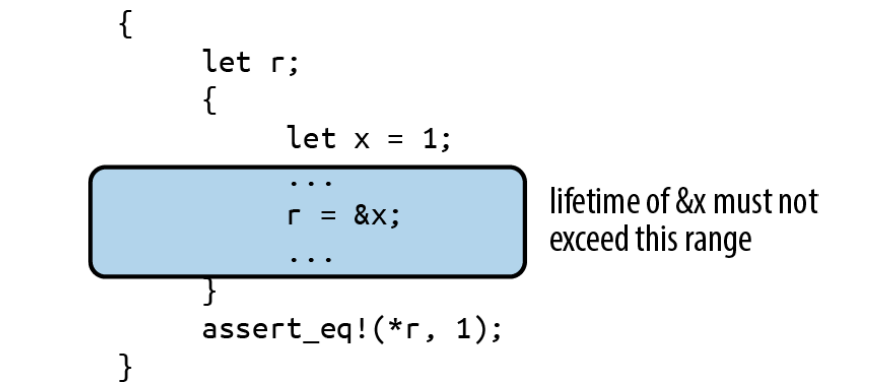
\includegraphics[width=0.9\textwidth]{../img/f5-3.png}
    \caption{\texttt{\&x}的合法生命周期}
    \label{f5-3}
\end{figure}

当\texttt{x}离开作用域之后,引用将变为悬垂指针。因此我们说变量的生命周期必须\emph{包含}或\emph{包括}它的引用的生命周期。

这里还有另一种约束:如果你把引用存储到变量\texttt{r}中,引用的生命周期必须覆盖变量的整个生命周期:从它初始化到最后一次使用它,如\hyperref[f5-4]{图5-4}所示。

\begin{figure}[htbp]
    \centering
    \includegraphics[width=0.9\textwidth]{../img/f5-4.png}
    \caption{存储在\texttt{r}中的引用的合法生命周期}
    \label{f5-4}
\end{figure}

如果引用不能和变量生存的一样长,那么在某些区域内指针\texttt{r}会变成悬垂指针。因此我们说引用的生命周期必须包含或包括存储它的变量的生命周期。

第一种约束限制了引用生命周期的上限,第二种约束限制了它的下限。Rust简单的尝试为每个引用找到一个满足这两个约束的生命周期。然而在我们的例子中,不存在这样的生命周期,如\hyperref[f5-5]{图5-5}所示。

\begin{figure}[htbp]
    \centering
    \includegraphics[width=0.9\textwidth]{../img/f5-5.png}
    \caption{一个引用的生命周期的限制互相矛盾}
    \label{f5-5}
\end{figure}

让我们考虑一个可以正常工作的不同的例子。我们有相同的约束:引用的生命周期必须被\texttt{x}的生命周期包含,但又要包含\texttt{r}的生命周期。但因为现在\texttt{r}的生命周期变小了,所以存在这样一个满足约束的生命周期,如\hyperref[f5-6]{图5-6}所示。

\begin{figure}[htbp]
    \centering
    \includegraphics[width=0.9\textwidth]{../img/f5-6.png}
    \caption{一个引用的生命周期包括\texttt{r}的生命周期、但被\texttt{x}的生命周期包含}
    \label{f5-6}
\end{figure}

当你借用一个更大的数据结构中的一部分的引用时这些规则也自然地生效,例如引用vector的一个元素:
\begin{minted}{Rust}
    let v = vec![1, 2, 3];
    let r = &v[1];
\end{minted}

因为\texttt{v}拥有vector,vector又拥有它的元素,所以\texttt{v}的生命周期必须包含引用\texttt{\&v[1]}的生命周期。类似的,如果你把引用存储在了某些数据结构之中,那引用的生命周期必须包含这个数据结构的生命周期。例如,如果你创建了一个引用的vector,那么每个引用的生命周期都必须包含拥有这个vector的变量的生命周期。

这是Rust对所有代码进行的实质的处理。如果考虑更多的语言特性——例如复杂的数据结构和函数调用,只是会引入新的约束,但核心原则是不变的:首先,理解程序使用引用的方式所带来的约束;然后,找到满足这些约束的生命周期。这与C和C++程序员给自己施加的限制没有太大区别,区别在于Rust自己知道这些规则并且强迫它们执行。

\subsection{引用作为函数参数}\label{RefAsArg}

我当我们向函数传递引用时,Rust怎么保证函数安全地使用它?假设我们有一个函数\texttt{f},这个函数接受一个引用,然后把它存储到一个全局变量中。我们之后会进行一些修改,不过这里有一个最初的版本:
\begin{minted}{Rust}
    // 这段代码有几个问题,不能通过编译。
    static mut STASH: &i32;
    fn f(p: &i32) { STASH = p; }
\end{minted}

Rust中的全局变量叫做\emph{静态变量}:它在程序开始时就被创建,直到程序终止时才被销毁。(类似其他的声明,Rust的模块系统控制静态变量在哪些部分可见,它们的“全局”只体现在生命周期上,而不是在可见性上)我们将在\hyperref[ch08]{第8章}中介绍静态变量,但现在我们只列出几条代码没有遵守的规则:
\begin{itemize}
    \item 每一个静态变量必须被初始化
    \item 可变的静态变量天然是线程不安全的(因为所有线程都可以在任何时间访问一个静态变量),即使在单线程程序中,它们也可能成为其它类型的重入问题的牺牲品。因为这些原因,你只能在\texttt{unsafe}块中使用可变的静态变量。在这个例子中我们并不关注那些特定的问题,我们只是把它放进\texttt{unsafe}块中,然后继续。
\end{itemize}

有了这些修改之后,我们有了下面的代码:
\begin{minted}{Rust}
    static mut STASH: &i32 = &128;
    fn f(p: &i32) { // 仍然不行
        unsafe {
            STASH = p;
        }
    }
\end{minted}

只差一步了,为了看到剩余的问题,我们需要写出一些Rust帮我们省略的东西。这里写的\texttt{f}的签名实际上是如下签名的缩写:
\begin{minted}{Rust}
    fn f<'a>(p: &'a i32) { ... }
\end{minted}

这里,生命周期\texttt{'a}(读作“tick A”)是\texttt{f}的一个\emph{生命周期参数}。你可以将\texttt{<'a>}读作“对于任何生命周期\texttt{'a}”,因此当我们写\texttt{fn f<'a>(p: \&'a i32)}时,我们定义了一个接受一个\texttt{i32}类型且带有任何给定生命周期\texttt{'a}的参数的函数。

尽管我们必须允许\texttt{'a}是任何生命周期,但如果它是最小的可能的生命周期的话会更好:例如恰好包含对\texttt{f}的调用。然后赋值语句就成了问题所在:
\begin{minted}{Rust}
    STASH = p;
\end{minted}

因为\texttt{STASH}在程序的整个执行过程中都存在,所以它持有的引用必须有相同长度的生命周期;Rust把这种生命周期称为\emph{\texttt{'static}生命周期}。但是\texttt{p}的生命周期是\texttt{'a},这意味着它可以是任何包含对\texttt{f}的调用的生命周期。因此,Rust拒绝了我们的代码:
\begin{minted}{text}
    error: explicit lifetime required in the type of `p`
      |
    5 | fn f(p: &i32) { // 仍然不行
      |         ____ help: add explicit lifetime `'static`
      |              to the type of `p`: `&'static i32`
    6 |     unsafe {
    7 |         STASH = p;
      |                 ^ lifetime `'static` required
\end{minted}

到这里,已经很明显了,我们的函数不能接受任意引用作为参数。但正如Rust指出的一样,它应该能接受一个有\texttt{'static}生命周期的引用:把这样一个引用存储到\texttt{STASH}不会导致悬垂指针。并且确实,下面的代码可以编译:
\begin{minted}{Rust}
    static mut STASH: &i32 = &10;

    fn f(p: &'static i32) {
        unsafe {
            STASH = p;
        }
    }
\end{minted}

这一次,\texttt{f}的签名指明了\texttt{p}必须是一个有\texttt{'static}生命周期的引用,因此将它存储在\texttt{STASH}中没有任何问题。我们只能将\texttt{f}用于其他静态变量的引用,但这是唯一一种保证\texttt{STASH}不会变为悬垂指针的方法。因此我们可以写:
\begin{minted}{Rust}
    static WORTH_POINTING_AT: i32 = 1000;
    f(&WORTH_POINTING_AT);
\end{minted}

因为\texttt{WORTH\_POINTING\_AT}是一个静态变量,所以\texttt{\&WORTH\_POINTING\_AT}的类型是\texttt{\&'static i32},可以安全地传递给\texttt{f}。

稍微后退一步,注意一下我们这种修改的方式让\texttt{f}的签名发生了什么变化:原本的\texttt{f(p: \&i32)}变为了\texttt{f(p: \&'static i32)}。换句话说,如果不在函数签名中表明我们的意图,我们将不能写出一个把引用存储在全局变量中的函数。在Rust中,一个函数的签名总是暴露出函数体的行为。

反过来说,如果我们看到了一个函数签名例如\texttt{g(p: \&i32)}(或者写出了生命周期的\texttt{g<'a>(p: \&'a i32)}),我们将能辨别出它\emph{不会}把参数\texttt{p}存储在此次调用之外的变量中。我们不需要查看\texttt{g}的定义,\texttt{g}的签名已经告诉了我们它能做什么和不能做什么。当你想保持函数调用的安全性时,这一点会很有用。

\subsection{向函数传递引用}
现在我们已经展示了一个函数的签名怎么和它的函数体关联起来,让我们继续解释它怎么和函数的调用者联系起来。假设你有下面的代码:
\begin{minted}{Rust}
    // 这可以被更简洁地写为:fn g(p: &i32)
    // 但现在让我们写出生命周期
    fn g<'a>(p: &'a i32) { ... }

    let x = 10;
    g(&x);
\end{minted}

仅仅从\texttt{g}的签名,Rust就知道它不会把\texttt{p}存储在生命周期超过此次调用的变量中:任何包含此次调用的生命周期\texttt{'a}都一定能正常工作。因此Rust为\texttt{\&x}选择了最小的可能的生命周期:也就是对\texttt{g}的调用。这满足了所有的约束:它的生命周期没有超过\texttt{x}、包含\texttt{g}的整个调用。因此这段代码可以通过检查。

注意尽管\texttt{g}有一个生命周期参数\texttt{'a},我们在调用\texttt{g}时不需要提到它。你只需要在定义函数和类型时担心生命周期参数,当使用它们时,Rust会为你推断生命周期。

如果我们尝试把\texttt{\&x}传递给之前的接受静态引用参数的\texttt{f}函数,会发生什么呢?
\begin{minted}{Rust}
    fn f(p: &'static i32) { ... }

    let x = 10;
    f(&x);
\end{minted}

这样会编译失败:引用\texttt{\&x}不能生存的比\texttt{x}更久,但传递给\texttt{f}时,我们约束它至少要和\texttt{'static}生存的一样久。没有办法同时满足所有约束,所以Rust会拒绝这段代码。

\subsection{返回引用}
一种很常见的场景是一个函数接受一些数据结构的引用,然后返回一个指向这个结构中部分数据的引用。例如,这里有一个函数返回一个切片中最小的元素的引用:
\begin{minted}{Rust}
    // v应该至少有一个元素
    fn smallest(v: &[i32]) -> &i32 {
        let mut s = &v[0];
        for r in &v[1..] {
            if *r < *s { s = r; }
        }
        s
    }
\end{minted}

我们按照通常的方式省略了函数签名中的生命周期参数。当一个函数接收单个引用作为参数并返回单个引用时,Rust假设这两个引用一定有相同的生命周期。如果显式写出生命周期将是:
\begin{minted}{Rust}
    fn smallest<'a>(v: &'a [i32]) -> &'a i32 { ... }
\end{minted}

假设我们像这样调用\texttt{smallest}:
\begin{minted}{Rust}
    let s;
    {
        let parabola = [9, 4, 1, 0, 1, 4, 9];
        s = smallest(&parabola);
    }
    assert_eq!(*s, 0);  // 错误:s指向的元素已经被drop
\end{minted}

通过\texttt{smallest}的签名,我们能看出它的参数和返回值必须有相同的生命周期\texttt{'a}。在我们的调用中,参数\texttt{\&parabola}不能比\texttt{parabola}生存的久,然而\texttt{smallest}的返回值又至少要和\texttt{s}生存的一样久。不存在生命周期\texttt{'a}可以同时满足这两个约束,因此Rust拒绝了代码:
\begin{minted}{text}
    error: `parabola` does not live long enough
      --> references_lifetimes_propagated.rs:12:5
       |
    11 |         s = smallest(&parabola);
       |                       -------- borrow occurs here
    12 |     }
       |     ^ `parabola` dropped here while still borrowed
    13 |     assert_eq!(*s, 0); // bad: points to element of dropped array
       |                 - borrowed value needs to live until here
    14 | }
\end{minted}

移动对\texttt{s}的使用来保证它的生命周期被\texttt{parabola}的生命周期包含可以解决这个问题:
\begin{minted}{Rust}
    {
        let parabola = [9, 4, 1, 0, 1, 4, 9];
        let s = smallest(&parabola);
        assert_eq!(*s, 0);  // fine: parabola still alive
    }
\end{minted}

函数签名中的生命周期让Rust能获得传进函数的引用和函数返回的引用的关系,然后保证它们都被安全地使用。

\subsection{包含引用的结构体}\label{refstruct}

Rust怎么处理存储在数据结构中的引用?这里有一个我们之前看到的错误的程序,不过现在我们把它存在了一个结构体中:
\begin{minted}{Rust}
    // 不能通过编译
    struct S {
        r: &i32
    }
    
    let s;
    {
        let x = 10;
        s = S { r: &x };
    }
    assert_eq!(*s.r, 10);   // bad: reads from dropped `x`
\end{minted}

Rust对引用安全的约束不可能因为我们把引用藏在了结构体里就神奇的消失。这些约束最终也会作用在\texttt{S}上。事实上,Rust是很多疑的:
\begin{minted}{text}
    error[E0106]: missing lifetime specifier
     --> references_in_struct.rs:7:12
      |
    7 |         r: &i32
      |            ^ expected lifetime parameter
\end{minted}

当一个引用类型出现在其他类型的定义中时,你必须写出它的生命周期。你可以这样写:
\begin{minted}{Rust}
    struct S {
        r: &'static i32
    }
\end{minted}

这意味着\texttt{r}只能指向生命周期等于整个程序的\texttt{i32}值,这样限制太大了,替代方案是给类型一个生命周期参数\texttt{'a}并用于\texttt{r}:
\begin{minted}{Rust}
    struct S<'a> {
        r: &'a i32
    }
\end{minted}

现在类型\texttt{S}也有了一个生命周期,就像引用类型一样。你创建的每一个类型\texttt{S}的值都有一个新的生命周期\texttt{'a},它会成为你使用值的约束。你存储在\texttt{r}中的引用的生命周期需要包含\texttt{'a},\texttt{'a}需要包含存储这个\texttt{S}的变量的生命周期。

回到之前的代码,表达式\texttt{S \{ r: \&x \}}创建了一个生命周期为\texttt{'a}的新\texttt{S}。当你把\texttt{\&x}存储到\texttt{r}字段时,你约束了\texttt{'a}的生命周期必须被\texttt{x}的生命周期包含。

赋值语句\texttt{s = S { ... }}把\texttt{S}存储到了变量中,变量的生命周期直到示例的结尾处,\texttt{'a}的生命周期需要包含\texttt{s}的生命周期。现在Rust遇到了和之前一样的矛盾的约束:\texttt{'a}的生命周期不能超过\texttt{x},但又要至少和\texttt{s}一样长。没有满足条件的生命周期存在,所以Rust拒绝了这段代码。避免了灾难!

如果把带有生命周期参数的类型存储在其他类型里会发生什么?
\begin{minted}{Rust}
    struct D {
        s: S // not adequate
    }
\end{minted}

Rust是多疑的,正如我们在不指明生命周期的情况下把引用存储在\texttt{S}中一样:
\begin{minted}{Rust}
    error[E0106]: missing lifetime specifier
      |
    8 |     s: S // not adequate
      |        ^ expected named lifetime parameter
      |
\end{minted}

我们不能在这里省略\texttt{S}的生命周期:Rust需要知道\texttt{D}的生命周期和\texttt{S}中的引用的生命周期的关系,这样才能对\texttt{D}进行和对\texttt{S}、普通引用一样的检查。

我们可以给\texttt{s}加上\texttt{'static}生命周期,就可以编译了:
\begin{minted}{Rust}
    struct D {
        s: S<'static>
    }
\end{minted}

有了这个定义之后,\texttt{S}字段只能借用生命周期等于整个程序的值。这太严格了,它意味着\texttt{D}不能借用本地变量,\texttt{D}的生命周期没有特殊的限制。

Rust的错误信息建议了另一种更通用的解决方法:
\begin{minted}{text}
    help: consider introducing a named lifetime parameter
      |
    7 | struct D<'a> {
    8 |     s: S<'a>
      |
\end{minted}

这里,我们给了\texttt{D}自己的生命周期参数并传递给\texttt{S}:
\begin{minted}{Rust}
    struct D<'a> {
        s: S<'a>
    }
\end{minted}

通过接受一个生命周期参数\texttt{'a}并把它用于\texttt{s}的类型,我们就可以允许Rust把\texttt{D}的值的生命周期关联到它持有的\texttt{S}的生命周期。

我们之前展示了函数的签名怎么暴露出它对传入的引用的操作。现在我们展示了关于类型的相似之处:一个类型的生命周期参数总是表明它是否持有一些带有有趣的(也就是非\texttt{'static}的)生命周期的引用,以及这些生命周期是什么样的。

例如,假设我们有一个解析函数,这个函数接受一个字节切片,返回一个保存解析结果的结构体:
\begin{minted}{Rust}
    fn parse_record<'i>(input: &'i [u8]) -> Record<'i> { ... }
\end{minted}

根本不需要查看\texttt{Record}类型的定义,我们就可以判断出,如果我们获得了一个\\
\texttt{parse\_record}返回的\texttt{Record},那么它里面包含的引用一定指向我们传入的缓冲区内的内容,而不是别的东西(除了可能的\texttt{'static}值)。

事实上,这种内部行为的暴露是Rust要求持有引用的类型显式写出生命周期参数的主要原因。否则,Rust完全可以为结构体中的每个引用标注一个不同的生命周期,让你可以省去写出它们的麻烦。早期版本的Rust确实是这么做的,但开发者发现这样会让人很迷惑。知道一个值什么时候从另一个值里借用了部分内容是很有用的,特别是解决bug时。

不只有引用和像\texttt{S}这样的类型才有生命周期。Rust中的每个类型都有生命周期,包括\texttt{i32}和\texttt{String}。大多数都是简单的\texttt{'static},意味着这些类型的值想要生存多久就能生存多久。例如,一个\texttt{Vec<i32>}是自包含的,不需要在其他任何值离开作用于之前drop。而一个类型例如\texttt{Vec<\&'a i32>}的生命周期必须被\texttt{'a}包含:在它引用的值离开作用域之前它必须被drop。

\subsection{不同的生命周期参数}\label{DistLife}
假设你定义了一个类似这样的包含两个引用的结构体:
\begin{minted}{Rust}
    struct S<'a> {
        x: &'a i32,
        y: &'a i32,
    }
\end{minted}

这两个引用的生命周期都是\texttt{'a}。如果你想像下面这样做的话这可能会是一个问题:
\begin{minted}{Rust}
    let x = 10;
    let r;
    {
        let y = 20;
        {
            let s = S { x: &x, y: &y };
            r = s.x;
        }
    }
    println!("{}", r);
\end{minted}

这段代码不会制造任何悬垂指针。对\texttt{y}的引用存储在\texttt{s}中,\texttt{s}在\texttt{y}离开作用于之前先离开作用域。\texttt{x}的引用随着\texttt{r}结束,没有超过\texttt{x}的生命周期。

然而,如果你尝试编译这段代码,Rust会报错说\texttt{y}生存的不够久,尽管显然它的生命周期已经够了。

Rust为什么会报错?如果你仔细思考这段代码,你会发现以下原因:
\begin{itemize}
    \item \texttt{s}的两个字段都有相同的生命周期\texttt{'a},所以Rust必须找到一个生命周期同时适用于\texttt{s.x}和\texttt{s.y}。
    \item 我们进行了赋值\texttt{r = s.x},这要求\texttt{'a}必须包含\texttt{r}的生命周期。
    \item 我们用\texttt{\&y}初始化了\texttt{s.y},这要求\texttt{'a}必须不超过\texttt{y}的生命周期。
\end{itemize}

这些约束不可能同时满足:没有生命周期比\texttt{y}的作用域短又比\texttt{r}的长。所以Rust报错了。

问题出现的原因是\texttt{S}中的两个引用有相同的生命周期\texttt{'a}。将\texttt{S}的定义修改为每个引用有一个不同的生命周期就可以解决问题:
\begin{minted}{Rust}
    struct S<'a, 'b> {
        x: &'a i32,
        y: &'b i32
    }
\end{minted}

有了这个定义,\texttt{s.x}和\texttt{s.y}就有了独立的生命周期。我们对\texttt{s.x}做什么都不会影响我们存储在\texttt{s.y}中的值,因此现在可以很容易地满足约束:\texttt{'a}可以直接是\texttt{r}的生命周期,\texttt{'b}是\texttt{s}的生命周期(\texttt{y}的生命周期也可以用作\texttt{'b},但Rust尝试选择最小的满足条件的生命周期)。这样一切都没有问题了。

函数的签名也可以有相似的效果。假设我们有一个类似这样的函数:
\begin{minted}{Rust}
    fn f<'a>(r: &'a i32, s: &'a i32) -> &'a i32 { r } // perhaps too tight
\end{minted}

这里,两个生命周期参数使用了相同的生命周期\texttt{'a},这可能会像我们之前展示的一样对调用者施加不必要的约束。如果这导致了问题,你可以让每个参数都有独立的生命周期:
\begin{minted}{Rust}
    fn f<'a, 'b>(r: &'a i32, s: &'b i32) -> &'a i32 { r } // looser
\end{minted}

这样的缺点是添加生命周期可能会导致类型和函数类型更难阅读。你们可以先尝试最简单的定义然后逐渐放松限制直到代码能够编译。因为Rust不允许不安全的代码,等Rust告诉你哪有问题然后再去修复是一个完美的策略。

\subsection{省略生命周期参数}\label{OmitLifeTime}
目前为止我们已经展示了足够多的返回引用或获取引用参数的函数,但我们通常不需要写出哪个生命周期是哪个。当生命周期很明显的时候Rust让我们可以省略它们。

在最简单的例子中,你可能永远都不需要写出参数的生命周期。Rust会为每一个需要声明周期的位置分配一个生命周期。例如:
\begin{minted}{Rust}
    struct S<'a, 'b> {
        x: &'a i32,
        y: &'b i32
    }

    fn sum_r_xy(r: &i32, s: S) -> i32 {
        r + s.x + s.y
    }
\end{minted}

这个函数签名是如下的缩写:
\begin{minted}{Rust}
    fn sum_r_xy<'a, 'b, 'c>(r: &'a i32, s: S<'b, 'c>) -> i32
\end{minted}

如果你返回了带有生命周期的参数的引用或其它类型,Rust仍会尝试允许无歧义的情况下省略。如果你的函数参数中只有一个生命周期参数,那么Rust会假设你的返回值中的所有生命周期参数都是那一个:
\begin{minted}{Rust}
    fn first_third(point: &[i32; 3]) -> (&i32, &i32) {
        (&point[0], &point[2])
    }
\end{minted}

如果把所有的生命周期参数都写出来,那么等价的代码如下:
\begin{minted}{Rust}
    fn first_third<'a>(point: &'a [i32; 3]) -> (&'a i32, &'a i32)
\end{minted}

如果参数里有多个生命周期参数,编译器没有简单的方法推断出返回值中的生命周期参数是哪个,此时Rust会要求你指明。

如果你的函数是某个类型的方法,并通过引用获取\texttt{self}参数,那么会打破这个限制:Rust会假设是返回值中所有内容的生命周期都和\texttt{self}的生命周期相同。(Rust中的\texttt{self}参数代表调用这个方法的值,等价于C++、Java、JavaScript中的\texttt{this},或者Python中的\texttt{self}。我们将在\hyperref[method]{使用impl定义方法}一节中介绍方法。)

例如,你可以写如下代码:
\begin{minted}{Rust}
    struct StringTable {
        elements: Vec<String>,
    }

    impl StringTable {
        fn find_by_prefi(&self, prefix: &str) -> Option<&String> {
            for i in 0 .. self.elements.len() {
                if self.elements[i].starts_width(prefix) {
                    return Some(&self.elements[i]);
                }
            }
            None
        }
    }
\end{minted}

\texttt{find\_by\_prefix}方法的签名是如下签名的缩写:
\begin{minted}{Rust}
    fn find_by_prefix<'a, 'b>(&'a self, prefix: &'b str) -> Option<&'a String>
\end{minted}
Rust假设如果你要借用,那么你会从\texttt{self}借用。

同样,这些只是缩写,用来提供帮助,并不能带来惊喜。如果它们不是你想要的,你可以显式写出生命周期。

\section{共享vs可变}\label{ShareVSMut}

到目前为止,我们已经讨论了Rust如何保证没有引用会指向已经离开作用域的变量。但还有其它方法造成悬垂指针。这里有一个简单的例子:
\begin{minted}{Rust}
    let v = vec![4, 8, 19, 27, 34, 10];
    let r = &v;
    let aside = v;  // 将vector移动到aside
    r[0];           // bad:使用了`v`,`v`未初始化
\end{minted}

对\texttt{aside}的赋值会移动vector,将\texttt{v}设为未初始化,因此\texttt{r}变成了一个悬垂指针。如\hyperref[f5-7]{图5-7}所示。

\begin{figure}[htbp]
    \centering
    \includegraphics[width=0.9\textwidth]{../img/f5-7.png}
    \caption{一个已经被移动的vector的引用}
    \label{f5-7}
\end{figure}

尽管\texttt{r}的整个生命周期内\texttt{v}都还在作用域之内,但问题是\texttt{v}的值被移动走了,\texttt{v}变为了未初始化,而\texttt{r}仍然指向它。自然,Rust捕捉到了这个错误:
\begin{minted}{text}
    error[E0505]: cannot move out of `v` because it is borrowed
      --> references_sharing_vs_mutation_1.rs:10:9
       |
    9  |     let r = &v;
       |              _ borrow of `v` occurs here
    10 |     let aside = v; // move vector to aside
       |         ^^^^^ move out of `v` occurs here
\end{minted}

在一个共享引用的整个生命周期内,它会使它引用的值只读:你不能对引用的值赋值或者移动它的值。在这段代码中,\texttt{r}的生命周期包括尝试移动vector的语句,因此Rust拒绝了这段代码。如果你按照下面这样修改,就不会有问题了:
\begin{minted}{Rust}
    let v = vec![4, 8, 19, 27, 34, 10];
    {
        let r = &v;
        r[0];   // ok: vector is still there
    }
    let aside = v;
\end{minted}

在这个版本中,\texttt{r}更早离开作用域,在\texttt{v}被移动之前引用的生命周期就结束了,因此没有任何问题。

这里还有一种导致问题的方式。假设我们有一个函数用一个切片里的元素扩展一个vector:
\begin{minted}{Rust}
    fn extend(vec: &mut Vec<f64>, slice: &[f64]) {
        for elt in slice {
            vec.push(*elt);
        }
    }
\end{minted}

这是标准库里vector的\texttt{extend\_from\_slice}的一种不够灵活(也不够优化)的版本。我们可以使用它从其他vector或数组的切片构建vector:
\begin{minted}{Rust}
    let mut wave = Vec::new();
    let head = vec![0.0, 1.0];
    let tail = [0.0, -1.0];

    extend(&mut wave, &head);   // 用另一个vector扩展wave
    extend(&mut wave, &tail);   // 用一个数组扩展wave

    assert_eq!(wave, vec![0.0, 1.0, 0.0, -1.0]);
\end{minted}

这里我们构建了正弦波的一个周期。如果我们想再添加一个周期,我们可以把vector附加给它自己吗?
\begin{minted}{Rust}
    extend(&mut wave, &wave);
    assert_eq!(wave, vec![0.0, 1.0, 0.0, -1.0,
                          0.0, 1.0, 0.0, -1.0]);
\end{minted}

粗略地检查一遍,感觉这好像没有问题。但记住当我们把元素添加到vector中时,如果缓冲区已经满了,它必须重新分配一个更大的缓冲区。假设\texttt{wave}一开始有4个元素,因此当\texttt{extend}尝试添加第5个元素时\texttt{wave}必须分配更大的缓冲区。此时内存布局看起来如\hyperref[f5-8]{图5-8}.

\begin{figure}[htbp]
    \centering
    \includegraphics[width=0.8\textwidth]{../img/f5-8.png}
    \caption{vector重新分配内存导致一个切片变为悬垂指针}
    \label{f5-8}
\end{figure}

\texttt{extend}函数的\texttt{vec}参数借用了\texttt{wave},\texttt{wave}已经分配了一个有8个元素的缓冲区,而\texttt{slice}仍然指向旧的4个元素的缓冲区,但这个缓冲区已经被drop了。

这种问题不是Rust独有的:在指向集合的同时修改集合在很多语言里都是很微妙的领域。在C++中,\texttt{std::vector}的规范提醒你“[vector的缓冲区的]重新分配会导致所有其中的元素的引用、指针、迭代器无效”。类似的,Java中有关修改\texttt{java.util.Hashtable}对象是这么说的:

\hangparagraph{\emph{如果创建了Hashtable的迭代器之后,Hashtable被修改了,除了迭代器自身的remove方法之外,任何操作都会导致迭代器抛出一个\texttt{ConcurrentModificationException}异常。}}

导致这种bug特别难解决的是它并不是总是发生。在测试中,你的vector可能总是恰好有足够的空间,缓冲区从来不重新分配,那这个问题可能一直都不会被曝光。

然而Rust,会在编译期就汇报调用\texttt{extend}的问题:
\begin{minted}{text}
    error[E0502]: cannot borrow `wave` as immutable because it is also
    borrowed as mutable
     --> references_sharing_vs_mutation_2.rs:9:24
      |
    9 |     extend(&mut wave, &wave);
      |                 ----   ^^^^ mutable borrow ends here
      |                 |      |
      |                 |      immutable borrow occurs here
      |                 mutable borrow occurs here
\end{minted}

换句话说,我们可以借用vector的可变引用,也可以借用它的元素的共享引用,但这两种引用的生命周期不能有重叠的部分。在我们的例子中,两个引用的生命周期都包含\texttt{extend}的调用,所以Rust拒绝了这段代码。

这些错误都违背了Rust关于可变和共享的核心规则:

\begin{flushleft}
    \emph{共享访问是只读的访问}
\end{flushleft}

\hangparagraph{共享引用借用的值是制度的。在一个共享引用的生命周期中,不管是它引用的值,还是任何通过这个值可以访问的东西,都不能被\emph{任何东西}修改。如果一个结构体的所有者是只读的,将不允许指向结构体中任何内容的可变引用。它实际上被冻结了。}

\begin{flushleft}
    \emph{可变访问是独占的访问}
\end{flushleft}

\hangparagraph{可变引用借用的值只能通过这个引用访问。在一个可变引用的生命周期内,没有任何其他方法访问被引用的值或通过这个值可以访问到的值。唯一能与可变引用的生命周期出现重叠的引用就是那个可变引用自己。}

Rust会报告\texttt{extend}的例子违反了第二条规则:因为我们已经借用了\texttt{wave}的一个可变引用,这个可变引用必须是唯一访问vector和它的元素的方法。切片的共享引用是另一种访问元素的方式,因此违反了第二条规则。

但Rust也可以把我们的bug当成违反了第一条规则:因为我们已经获取了\texttt{wave}的元素的共享引用,元素和\texttt{Vec}自身都变为只读,所以你不能再借用一个只读值的可变引用。

每种引用都会影响我们可以对被引用的值,以及通过这个值可以访问的值进行的操作(\hyperref[f5-9]{图5-9})。

\begin{figure}[htbp]
    \centering
    \includegraphics[width=0.9\textwidth]{../img/f5-9.png}
    \caption{借用一个引用会影响你可以对同一棵所有权树中的其他值进行的操作}
    \label{f5-9}
\end{figure}

注意在两种情况下,在引用的生命周期内,所有权树中通往被引用值的路径都不可能被修改。对于共享引用,这个路径是只读的;对于一个可变引用,这个路径完全不可访问。因此一个程序没有任何方法让一个引用变的无效。

将这些原则分解为最简单的示例:
\begin{minted}{Rust}
    let mut x = 10;
    let r1 = &x;
    let r2 = &x;    // ok:允许多个共享引用
    x += 10;        // error:不能对`x`赋值因为它已经被借用了
    let m = &mut x; // error:不能借用`x`的可变引用,
                    // 因为它已经被借用了不可变引用
    println!("{}, {}, {}", r1, r2, m); // 引用都在这里使用
                                       // 因此它们的生命周期
                                       // 都只到这里

    let mut y = 20;
    let m1 = &mut y;
    let m2 = &mut y;    // error:不能再次借用可变引用
    let z = y;          // error:不能使用`y`,因为它被借用了可变引用
    println!("{}, {}, {}", m1, m2, z);  // 引用都在这里使用
\end{minted}

可以从一个共享引用借用一个共享引用:
\begin{minted}{Rust}
    let mut w = (107, 109);
    let r = &w;
    let r0 = &r.0;          // ok;从共享引用再次借用共享引用
    let m1 = &mut r.1;      // error:不能从共享引用借用可变引用
    println!("{}", r0);     // r0在这里使用
\end{minted}

也可以再次借用一个可变引用:
\begin{minted}{Rust}
    let mut v = (136, 139);
    let m = &mut v;
    let m0 = &mut m.0;      // ok:从可变引用重新借用可变引用
    *m0 = 137;
    let r1 = &m.1;          // ok:从可变引用重新借用共享引用
                            // 并且和m0没有重叠部分
    v.1;                    // error:通过其他路经访问仍然是禁止的
    println!("{}", r1);     // r1在这里使用
\end{minted}

这些限制非常严格。回到我们调用\texttt{extend(\&mut wave, \&wave)}的地方,没有方便快速的方法修复代码让它按我们希望的方式运行。Rust在几乎所有地方应用这些规则:如果我们借用了一个\texttt{HashMap}里的一个键的共享引用,我们将不能借用整个\texttt{HashMap}的可变引用,直到共享引用的生命周期结束。

但有足够的理由这么做:设计一个支持不严格的、可以同时迭代和修改的集合是非常困难的,并且通常没有简单高效的实现。Java的\texttt{Hashtable}和C++的\texttt{vector}并不考虑这些、Python的字典、JavaScript的对象也没有定义这种情况下的行为。JavaScript中的其它集合类型做到了这一点,但也导致了更加笨重的实现。C++的\texttt{std::map}承诺插入新的条目不会使指向map中其他条目的指针失效,但为了实现这个承诺,标准中排除了类似Rust中的\texttt{BTreeMap}的更加缓存高效的实现,这种实现在树中的每个节点存储多个条目。

这里有另一个这些规则可以捕获的bug的例子。考虑下面的C++代码,用于管理一个文件描述符。为了保持简单,我们只写出构造函数和一个拷贝赋值运算符,并且省略错误处理:
\begin{minted}{C++}
    struct File {
        int descriptor;

        File(int d) : descriptor(d) { }

        File& operator=(const File &rhs) {
            close(descriptor);
            descriptor = dup(rhs.descriptor);
            return *this;
        }
    }
\end{minted}

赋值运算符足够简单,但在像这样的特殊情况下会出现问题:
\begin{minted}{C++}
    File f(open("foo.txt", ...));
    ...
    f = f;
\end{minted}

如果们把一个\texttt{File}赋给它自己,那么\texttt{rhs}和\texttt{*this}是同一个对象,因此\texttt{operator=}会关闭它准备\texttt{dup}的文件描述符。我们销毁了想要拷贝的资源。

在Rust中,类似的代码将是:
\begin{minted}{Rust}
    struct File {
        descriptor: i32
    }

    fn new_file(d: i32) -> File {
        File { descriptor: d }
    }

    fn clone_from(this: &mut File, rhs: &File) {
        close(this.descriptor);
        this.descriptor = dup(rhs.descriptor);
    }
\end{minted}
(这并不是Rust中的常用写法。Rust有优秀的方法给Rust中的类型添加构造函数和方法,我们将在\hyperref[ch09]{第9章}介绍,但上面的定义对这个例子来说已经足够了。)

如果我们写出与之前使用\texttt{File}相对应的Rust代码,我们有:
\begin{minted}{Rust}
    let mut f = new_file(open("foo.txt", ...));
    ...
    clone_from(&mut f, &f);
\end{minted}

当然,Rust拒绝编译代码:
\begin{minted}{text}
    error[E0502] : cannot borrow `f` as immutable because it is also 
    borrowed as mutable 
      --> references_self_assignment.rs:18:25
       |
    18 |     clone_from(&mut f, &f);
       |                     -   ^- mutable borrow ends here 
       |                     |   |
       |                     |   immutable borrow occurs here 
       |                     mutable borrow occurs here
\end{minted}

这看起来很熟悉。它暴露出了两种典型的C++ bug——无法处理自我赋值以及使用无效的迭代器——两者实际上是同一种底层类型的bug!在这两种情况下,代码都假设它在修改一个值的同时访问另一个值,然而实际上它们是同一个值。如果你曾经偶然在C和C++中让\texttt{memcpy}或\texttt{strcpy}的调用的源区间和目标区间重叠,那么将会产生另一种形式的bug。通过要求可变引用必须独占,Rust可以避免各种各样的日常错误。

共享和可变引用的互斥实际上也展示了编写并发代码时值的状态。只有当值在某些线程中既可写又共享时才可能发生数据竞争——Rust的引用规则恰好可以避免这种情况。没有\texttt{unsafe}代码的并发Rust程序可以\emph{从构造上}完全避免数据竞争。我们将在\hyperref[ch19]{第19章}中详细介绍更多有关并发的细节。但总的来说,在Rust中使用并发要比大多数其他语言轻松得多。

\clearpage

\definecolor{shadecolor}{RGB}{240, 240, 240}
\begin{shaded}
    \begin{center}
        \Large{Rust的共享引用 vs C的常量指针}
    \end{center}

    乍一看,Rust中的共享引用很向C和C++中指向\texttt{const}值的指针。然而,Rust对共享引用的限制要更严格。例如考虑下面的C代码:
    \begin{minted}{C}
    int x = 42;         // int变量,不是const
    const int *p = &x;  // 指向const int的指针
    assert(*p == 42);
    x++;                // 直接修改变量
    assert(*p == 43);   // “常量”的int值已经被修改了
    \end{minted}

    \texttt{p}是\texttt{const int *}的事实意味着你不能通过\texttt{p}自身来改变它指向的值:\texttt{(*p)++}是禁止的。但你可以直接通过\texttt{x}访问被引用的值,而\texttt{x}并不是\texttt{const},所以你可以直接修改它的值。C家族的\texttt{const}关键字有它的作用,但它并不能把指向的值变为常量。

    在Rust中,一个共享引用会禁止对被引引用值的任何修改,直到引用的生命周期结束:
    \begin{minted}{Rust}
    let mut x = 42;         // 非常量i32值
    let p = &x;             // i32的共享引用
    assert_eq!(*p, 42);
    x += 1;                 // 错误:不能对x赋值因为它已经被借用了
    assert_eq!(*p, 42);     // 如果删除赋值语句,断言将为真
    \end{minted}

    为了确保值是常量,我们需要持续追踪所有可以访问到这个值的路径,并确保它们都不允许修改操作或者直接不可用。C和C++的编译器对指针的检查太过宽松。Rust的引用总是关联到一个特定的生命周期,这使得在编译期检查它们变得可行。
\end{shaded}    

\clearpage

\section{拿起武器对抗对象之海}

自从19世纪90年代起自动内存管理兴起之后,所有程序的默认架构都变成了\emph{对象之海(sea of objects)},如\hyperref[f5-10]{图5-10}所示。

\begin{figure}[htbp]
    \centering
    \includegraphics[width=0.9\textwidth]{../img/f5-10.png}
    \caption{一个对象之海}
    \label{f5-10}
\end{figure}

这就是如果你不假思索就开始编写程序并且有垃圾回收时的真实情景。我们都在构建这样的系统。

这种架构有很多图中没有显示出的优势:初始化很快、很容易破译里面的逻辑、而且即使几年之后你也可以轻易的完全重写它们。(Cue AC/DC's “Highway to Hell.”(通往地狱的高速公路))。

当然,它也有很多缺陷。当每个东西都依赖别的任何东西的时候,将非常难以测试、推演、甚至单独考虑其中的任何一部分组件。

Rust迷人的一点就是Rust在通往地狱的高速公路上放了一条减速带。在Rust中需要花费大量的努力才能制造出环形引用——两个值互相包含指向彼此的引用。你必须使用智能指针例如\texttt{Rc}和\hyperref[intermut]{内部可变性}——一个我们还没有讲到的话题。Rust更喜欢指针、所有权、数据流朝一个方向流经整个系统,如\hyperref[f5-11]{图5-11}所示。

\begin{figure}[htbp]
    \centering
    \includegraphics[width=0.9\textwidth]{../img/f5-11.png}
    \caption{一棵值组成的树}
    \label{f5-11}
\end{figure}

我们现在提出这一点的原因是,在阅读完这一章之后,你可能会很自然的想通过\texttt{Rc}智能指针创造一片“结构体的海洋”,然后完全重现你熟悉的面向对象的模式。你不能立刻就完成这些,因为Rust的所有权模型会给你制造一些麻烦。解决方法是事先进行设计并构建更好的程序。

Rust就是把理解你的程序的痛苦从未来转移到了现在。它做的非常好:它不仅强迫你理解为什么你的程序是线程安全的,它甚至还能要求一些高层级的架构设计。

    \chapter{表达式}\label{ch06}

\emph{LISP programmers know the value of everything, but the cost of nothing}

\begin{flushright}
    ——Alan Perlis, epigram \#55
\end{flushright}

在本章中,我们将介绍Rust的\emph{表达式},它是构成Rust函数体和大部分Rust代码的构建块。本章将探索表达式的力量以及如何克服它的局限。我们还将介绍控制流,它在Rust中完全是以表达式为基础的,最后还要介绍Rust中的基本运算符如何单独和组合工作。

还有一些从技术角度应该划入这一类的概念,例如闭包和迭代器。但它们太过重要因此我们之后会用单独的章节介绍它们。现在,我们希望能用尽可能少的页数介绍尽可能多的语法。

\section{表达式语言}

Rust表面上看上去像C家族的语言,但这其实是一个误解。在C语言中,\emph{表达式}和\emph{语句}之间有很大的不同。表达式是一些像这样的代码:
\begin{minted}{C}
    5 * (fahr-32) / 9
\end{minted}
而语句则是像这样的:
\begin{minted}{C}
    for (; begin != end; ++begin) {
        if (*begin == target)
            break;
    }
\end{minted}
表达式有值,但语句没有。

Rust是一种\emph{表达式语言}。这意味着它遵循了起源于Lisp的传统,即表达式负责完成所有工作。

在C中,\texttt{if}和\texttt{switch}是语句。它们并不产生值,也不能被用在表达式中间。在Rust中,\texttt{if}和\texttt{match}\emph{可以}产生值。我们已经在\hyperref[ch02]{第2章}中看到过一个产生数字值的\texttt{match}表达式:
\begin{minted}{Rust}
    pixels[r * bounds.0 + c] =
        match escapes(Complex { re: point.0, im: point.1 }, 255) {
            None => 0,
            Some(count) => 255 - count as u8
        };
\end{minted}

一个\texttt{if}表达式可以用于初始化一个变量:
\begin{minted}{Rust}
    let status =
        if cpu.temperature <= MAX_TEMP {
            HttpStatus::Ok
        } else {
            HttpStatus::ServerError  // server melted
        };
\end{minted}

一个\texttt{match}表达式可以被用作函数或宏的参数:
\begin{minted}{Rust}
    println!("Inside the vat, you see {}.",
        match vat.contents {
            Some(brain) => brain.desc(),
            None => "nothing of interest"
        });
\end{minted}

这解释了Rust为什么没有C的三元运算符\texttt{(expr1 ? expr2 : expr3)}。在C中,它是一种类似\texttt{if}语句的表达式。但在Rust中这种写法是多余的,因为\texttt{if}表达式可以同时实现这两种功能。

C中的大部分控制流工具都是语句,而Rust中的控制流则全是表达式。

\section{优先级与结合性}

\hyperref[t6-1]{表6-1}总结了Rust的表达式语法。我们将在这一章中介绍所有这些表达式。运算符按照优先级从高到低的顺序列出。(类似于大多数编程语言,Rust使用\emph{运算符优先级}来决定当表达式中含有多个运算符时的运算顺序。例如,在表达式\texttt{limit < 2 * broom.size + 1}中,\texttt{.}运算符优先级最高,因此会先访问字段。)

\begin{longtable}{p{0.25\textwidth}p{0.35\textwidth}p{0.3\textwidth}}
    \caption{表达式}
    \label{t6-1} \\
    \hline
    \textbf{表达式类型} & \textbf{示例} & \textbf{相关trait} \\
    \hline
    数组字面量      & \texttt{[1, 2, 3]}         & \\
    重复数组字面量  & \texttt{[0; 50]}           & \\
    元组            & \texttt{(6, "crullers")}  & \\
    \cline{1-2}
    组合            & \texttt{(2 + 2)}             & \\
    块              & \texttt{\{ f(); g() \}}      & \\
    控制流表达式     & \texttt{if ok \{ f() \}}     & \\
                    & \texttt{if ok \{ 1 \} else \{ 0 \}}                   & \\
                    & \texttt{if let Some(x) = f() \{ x \} else \{ 0 \}}    & \\
                    & \texttt{match x \{ None => 0, \_ => 1 \}}             & \\
                    & \texttt{for v in e \{ f(v); \}}                       & \texttt{\hyperref[iter]{std::iter::IntoIterator}} \\
                    & \texttt{while ok \{ ok = f(); \}}                     & \\
                    & \texttt{while let Some(x) = it.next() \{ f(x); \}}    & \\
                    & \texttt{loop \{ next\_event(); \}}                    & \\
                    & \texttt{break}                  & \\
                    & \texttt{continue}               & \\
                    & \texttt{return 0}               & \\
    宏调用          & \texttt{println!("ok")}         & \\
    路径            & \texttt{std::f64::consts::PI}   & \\
    \cline{1-2}
    结构体字面量     & \texttt{Point \{x: 0, y: 0\}}     & \\
    \cline{1-2}
    元组字段访问    & \texttt{pair.0}   & \texttt{\hyperref[deref]{Deref}, \hyperref[deref]{DerefMut}} \\
    结构体字段访问  & \texttt{point.x}  & \texttt{\hyperref[deref]{Deref}, \hyperref[deref]{DerefMut}} \\
    方法调用       & \texttt{point.translate(50, 50)} & \texttt{\hyperref[deref]{Deref}, \hyperref[deref]{DerefMut}} \\
    函数调用       & \texttt{stdin()}   & \texttt{\hyperref[fn]{Fn(Arg0, ...) -> T}, \hyperref[fn]{FnMut(Arg0, ...) -> T}, \hyperref[fn]{FnOnce(Arg0, ...) -> T}} \\
    索引            & \texttt{arr[0]}   & \texttt{\hyperref[index]{Index}, \hyperref[index]{IndexMut}, \hyperref[deref]{Deref}, \hyperref[deref]{DerefMut}} \\
    \cline{1-2}
    错误检查        & \texttt{create\_dir("tmp")?}   & \\
    \cline{1-2}
    逻辑/位 NOT     & \texttt{!ok}  & \texttt{\hyperref[unop]{Not}} \\
    负             & \texttt{-num}  & \texttt{\hyperref[unop]{Neg}} \\
    解引用          & \texttt{*ptr} & \texttt{\hyperref[deref]{Deref}, \hyperref[deref]{DerefMut}} \\
    借用            & \texttt{\&val}    & \\
    \cline{1-2}
    类型转换    & \texttt{x as u32} & \\
    \cline{1-2}
    乘法        & \texttt{n * 2}    & \texttt{\hyperref[biop]{Mul}} \\
    除法        & \texttt{n / 2}    & \texttt{\hyperref[biop]{Div}} \\
    余数(取模) & \texttt{n \% 2}   & \texttt{\hyperref[biop]{Rem}} \\
    \hline
    加法        & \texttt{n + 1}    & \texttt{\hyperref[biop]{Add}} \\
    减法        & \texttt{n - 1}    & \texttt{\hyperref[biop]{Sub}} \\
    \hline
    左移        & \texttt{n << 1}   & \texttt{\hyperref[biop]{Shl}} \\
    右移        & \texttt{n >> 1}   & \texttt{\hyperref[biop]{Shr}} \\
    \hline
    位与        & \texttt{n \& 1}   & \texttt{\hyperref[biop]{BitAnd}} \\
    \hline
    位异或      & \texttt{n \^{} 1} & \texttt{\hyperref[biop]{BitXor}} \\
    \hline
    位或        & \texttt{n | 1}    & \texttt{\hyperref[biop]{BitOr}}  \\
    \hline
    小于        & \texttt{n < 1}    & \texttt{\hyperref[cmp]{std::cmp::PartialOrd}} \\
    小于等于    & \texttt{n <= 1}   & \texttt{\hyperref[cmp]{std::cmp::PartialOrd}} \\
    大于        & \texttt{n > 1}    & \texttt{\hyperref[cmp]{std::cmp::PartialOrd}} \\
    大于等于    & \texttt{n >= 1}   & \texttt{\hyperref[cmp]{std::cmp::PartialOrd}} \\
    等于        & \texttt{n == 1}   & \texttt{\hyperref[equal]{std::cmp::PartialEq}} \\
    不等于      & \texttt{n != 1}   & \texttt{\hyperref[equal]{std::cmp::PartialEq}} \\   
    \hline
    逻辑与      & \texttt{x.ok \&\& y.ok}       & \\
    \cline{1-2}
    逻辑或      & \texttt{x.ok || backup.ok}    & \\
    \cline{1-2}
    左闭右开区间 & \texttt{start .. stop}   & \\
    左闭右闭区间 & \texttt{start ..= stop}  & \\
    \cline{1-2}
    赋值        & \texttt{x = val}  & \\
    复合赋值    & \texttt{x *= 1}   & \texttt{\hyperref[assign]{MulAssign}} \\
                & \texttt{x /= 1}   & \texttt{\hyperref[assign]{DivAssign}} \\
                & \texttt{x \%= 1}  & \texttt{\hyperref[assign]{RemAssign}} \\
                & \texttt{x += 1}   & \texttt{\hyperref[assign]{AddAssign}} \\
                & \texttt{x -= 1}   & \texttt{\hyperref[assign]{SubAssign}} \\
                & \texttt{x <<= 1}  & \texttt{\hyperref[assign]{ShlAssign}} \\
                & \texttt{x >>= 1}  & \texttt{\hyperref[assign]{ShrAssign}} \\
                & \texttt{x \&= 1}  & \texttt{\hyperref[assign]{BitAndAssign}} \\
                & \texttt{x \^{}= 1}& \texttt{\hyperref[assign]{BitXorAssign}} \\
                & \texttt{x |= 1}   & \texttt{\hyperref[assign]{BitOrAssign}} \\
    \cline{1-2}
    闭包        & \texttt{|x, y| x + y} & \\
\end{longtable}

所有可以链式使用的运算符都是左结合的。也就是说,一条运算链例如\texttt{a - b - c}被组合为\texttt{(a - b) - c},而不是\texttt{a - (b - c)}。这些运算符可以被任意组合:
\begin{minted}{text}
    * / % + - << >> & ^ | && || as
\end{minted}
比较运算符、赋值运算符、范围运算符\texttt{..}和\texttt{..=}不能被链式使用。

\section{块和分号}

块是最通用的表达式。一个块产生一个值,可以被用于任何需要一个值的地方:\begin{minted}{Rust}
    let display_name = match post.author() {
        Some(author) => author.name(),
        None => {
            let network_info = post.get_network_metadata()?;
            let ip = network_info.client_address();
            ip.to_string()
        }
    };
\end{minted}
\texttt{Some(author) =>}之后的代码是简单的表达式\texttt{author.name()},\texttt{None =>}之后的代码则是一个块表达式。对Rust来种,两种表达式没有区别。块表达式的值是它的最后一条表达式的值,也就是\texttt{ip.to\_string()}。

注意\texttt{ip.to\_string()}后面没有分号。Rust中的大部分代码行都以分号或者花括号结尾,类似于C和Java。如果一个块看起来像C代码一样在所有的表达式后边都有分号,那它的行为就和C块一样,它的值将是\texttt{()}。正如我们在\hyperref[ch02]{第2章}提到的,当你省略了块中最后一个表达式后边的分号,那么块的值将是最后一个表达式的值,而不是通常的\texttt{()}。

在一些语言中,尤其是Javascript,你可以省略分号,语言会自动为你添加上——这样除了方便一点,并没有任何区别。然而在Rust中,分号通常是有实际意义的:
\begin{minted}{Rust}
    let msg = {
        // let语句:总是需要分号
        let dandelion_control = puffball.open();

        // 表达式 + 分号:方法被调用,返回值被丢弃
        dandelion_control.release_all_seeds(launch_codes);

        // 没有分号的表达式:方法被调用,
        // 返回值被存储到 `msg`
        dandelion_control.get_status()
    };
\end{minted}

语句块可以包含声明最后还能产生一个值的能力是一个很有用的特性,而且可以很快习惯。它的一个缺陷是如果你偶然忘记了分号会导致一条错误信息:
\begin{minted}{Rust}
    ...
    if preferences.changed() {
        page.compute_size()  // oops, 缺少分号
    }
\end{minted}

如果你在C或者Java程序中犯了这种错误,编译器会简单地直接指出你少写了一个分号。然而这是Rust的报错:
\begin{minted}{text}
    error[E0308]: mismatched types
    22 |         page.compute_size()  // oops, missing semicolon
       |         ^^^^^^^^^^^^^^^^^^^- help: try adding a semicolon `;`
       |         |
       |         expected (), found tuple
       |
       = note: expected unit type `()`
                  found tuple `(u32, u32)`
\end{minted}

在缺少分号的情况下,块的值将是\texttt{page.compute\_size()}返回的值,但一个没有\texttt{else}分支的\texttt{if}语句必须总是返回\texttt{()}。幸运的是,Rust知道这种类型的错误并建议加上分号。

\section{声明}\label{declaration}

除了表达式和分号之外,一个块中可能包含任意数量的声明。最常见的情况是\texttt{let}声明,它用来声明局部变量:
\begin{minted}{Rust}
    let name: type = expr;
\end{minted}

类型和初始值是可选的,分号是必须的。

一个\texttt{let}声明可以在不初始化的情况下声明一个变量。这有时很有用,因为有时候一个变量需要在控制流的中途初始化:
\begin{minted}{Rust}
    let name;
    if user.has_nickname() {
        name = user.nickname();
    } else {
        name = generate_unique_name();
        user.register(&name);
    }
\end{minted}

局部变量\texttt{name}有两种不同的初始化路径,但两条路径上它都只会被初始化一次,所以\texttt{name}不需要声明为\texttt{mut}。

在变量初始化之前使用它会导致错误(这和使用被move的值的错误紧密相关,Rust希望你只在变量的值存在时使用它们!)。

你有时可能会看到代码似乎重新声明一个已经存在的变量,例如:
\begin{minted}{Rust}
    for line in file.lines() {
        let line = line?;
        ...
    }
\end{minted}

\texttt{let}声明创建了一个新的、类型不同的、第二个变量\texttt{line}。第一个\texttt{line}的类型是\\
\texttt{Result<String, io::Error>},第二个\texttt{line}是一个\texttt{String}。第二个声明在块的剩余部分会取代第一个。这被称为\emph{遮蔽(shadowing)},在Rust程序中非常常见。上面的代码等价于:
\begin{minted}{Rust}
    for line_result in file.lines() {
        let line = line_result?;
        ...
    }
\end{minted}

在本书中,我们将坚持在这种场景中使用\texttt{\_result}后缀,来保证变量的名字不同。

一个块还可以包含\emph{item declarations}。一个item是一个可以出现在全局或模块中的声明,例如\texttt{fn}、\texttt{struct}、\texttt{use}。

后面的章节将会详细介绍item。现在,\texttt{fn}足够作为一个例子了。任何块都可以包含\texttt{fn}声明:
\begin{minted}{Rust}
    use std::io;
    use std::cmp::Ordering;

    fn show_files() -> io::Result<()> {
        let mut v = vec![];
        ...
        fn cmp_by_timestamp_then_name(a: &FileInfo, b: &FileInfo) -> Ordering {
            a.timestamp.cmp(&b.timestamp)   // 首先,比较时间戳 
                .reverse()                  // 最新的文件优先
                .then(a.path.cmp(&b.path))  // 比较路径
        }

        v.sort_by(cmp_by_timestamp_then_name);
        ...
    }
\end{minted}

当一个\texttt{fn}在块内声明的时候,它的作用域是整个块,它可以在整个块内\emph{使用}。但是一个嵌套的\texttt{fn}不能访问外围作用域的局部变量和参数。例如,函数\texttt{cmp\_by\_timestamp\_then\_name}不能使用\texttt{v}。(Rust还有闭包,闭包可以使用外层作用域的变量,见\hyperref[ch14]{第14章}。)

一个块甚至可以包含整个模块。这听起来可能有些多余了:我们真的需要把语言的\emph{每一部分}嵌套在其他部分中的能力吗?——但程序员(尤其是使用宏的程序员)可以找到语言提供的每一个正交碎片的用法。

\section{\texttt{if}与\texttt{match}}

\texttt{if}表达式的形式大家都很熟悉:
\begin{minted}{Rust}
    if condition1 {
        block1
    } else if condition2 {
        block2
    } else {
        block_n
    }
\end{minted}

每一个\texttt{condition}都必须是\texttt{bool}类型的表达式,Rust不会隐式地将数字或者指针类型转换为布尔值。

和C不同的是条件表达式不需要括号,事实上如果有不必要的括号的话,\texttt{rustc}会发出警告。不过花括号是必须的。

\texttt{else if}块,和最后的\texttt{else}都是可选的。一个没有\texttt{else}块的\texttt{if}表达式类似于一个\texttt{else}块为空的\texttt{if}表达式。

\texttt{match}表达式有些类似于C的\texttt{switch}语句,但是更加灵活。一个简单的例子如下:
\begin{minted}{Rust}
    match code {
        0 => println!("OK"),
        1 => println!("Wires Tangled"),
        2 => println!("User Asleep"),
        _ => println!("Unrecognized Error {}", code)
    }
\end{minted}
这类似于一个\texttt{switch}语句,\texttt{match}表达式的四条分支里只有一条会执行,取决于\texttt{code}的值。通配符模式\texttt{\_}可以匹配任何情况,类似于\texttt{switch}语句中的\texttt{default:}标签,不过它会覆盖之后的所有模式,它之后的模式将永远不会匹配到任何东西(出现这种情况时编译器也会警告你)。

编译器可以使用跳转表来优化这种\texttt{match}表达式,类似于C++中的\texttt{switch}语句。当\texttt{match}\\
的每个分支都返回常量值时还会有一个类似的优化,这种情况下,编译器会用那些值构建一个数组,然后\texttt{match}会被编译为一次数组访问,这种情况下除了边界检查之外,编译出的代码将不会有任何条件分支。

每个分支中\texttt{=>}左侧支持多种\emph{模式},这是\texttt{match}功能强大的根源。上边的例子中,每种模式都只是一个简单的整数。我们还展示过区分\texttt{Option}的两种值的\texttt{match}表达式:
\begin{minted}{Rust}
    match params.get("name") {
        Some(name) => println!("Hello, {}!", name);
        None => println!("Greetings, stranger.");
    }
\end{minted}

这只是模式的一个小应用,一个模式可以匹配很多值。它可以解包元组,可以匹配结构体中的每个字段,可以解引用,借用一个值的一部分,等等。Rust的模式是一种专门的mini语言。我们将在\hyperref[ch10]{第10章}中介绍它们。

\texttt{match}表达式的通用形式是:
\begin{minted}{Rust}
    match value {
        pattern => expr,
        ...
    }
\end{minted}
如果\texttt{expr}是一个块的话,分支最后的逗号可以省略。

Rust会从第一个分支开始,逐个检查\texttt{value}和给定的模式是否匹配。当有一个模式匹配时,相应的\texttt{expr}将会被求值,整个\texttt{match}表达式将完成执行,不会再检查别的模式。必须至少有一个模式可以匹配,Rust会禁止没有覆盖所有可能情况的\texttt{match}表达式:
\begin{minted}{Rust}
    let score = match card.rank {
        Jack => 10,
        Queen => 10,
        Ace => 11
    };  // 错误:没有穷尽所有模式
\end{minted}

\texttt{if}表达式的所有块必须产生相同类型的值:
\begin{minted}{Rust}
    let suggested_pet = 
        if with_wings { Pet::Buzzard } else { Pet::Hyena }; // ok
    let favorite_number =
        if user.is_hobbit() { "eleventy-one" } else { 9 };  // error
    let best_sports_team = 
        if is_hockey_season() { "Predators" };  // error
\end{minted}
(最后一个例子会导致错误,因为在7月结果将是\texttt{()}。)\footnote{译者注:7月不是曲棍球赛季?}

类似的,\texttt{match}表达式的分支也必须有相同的类型:
\begin{minted}{Rust}
    let suggested_pet =
        match favorite.element {
            Fire => Pet::RedPanda,
            Air => Pet::Buffalo,
            Water => Pet::Orca,
            _ => None   // 错误:类型不一致
        }
\end{minted}

\section{\texttt{if let}}\label{iflet}

\texttt{if}表达式还有一种形式:\texttt{if let}表达式:
\begin{minted}{Rust}
    if let pattern = expr {
        block1
    } else {
        block2
    }
\end{minted}

\texttt{expr}如果能匹配\texttt{pattern},则执行\texttt{block1},如果不能匹配,则执行\texttt{block2}。有时这是一种获取\texttt{Option}或\texttt{Result}的值的好方法:
\begin{minted}{Rust}
    if let Some(cookie) = request.session_cookie {
        return restore_session(cookie);
    }

    if let Err(err) = show_cheesy_anti_robot_task() {
        log_robot_attempt(err);
        politely_accuse_user_of_being_a_robot();
    } else {
        session.mark_as_human();
    }
\end{minted}

没有任何场景\emph{必须}使用\texttt{if let},因为\texttt{match}可以做到任何\texttt{if let}可以做的事。\texttt{if let}表达式类似于如下只有一个模式的\texttt{match}表达式的缩写:
\begin{minted}{Rust}
    match expr {
        pattern => { block1 }
        _ => { block2 }
    }
\end{minted}

\section{循环}\label{loop}

有四种循环表达式:
\begin{minted}{Rust}
    while condition {
        block
    }
    
    while let pattern = expr {
        block
    }

    loop {
        block
    }

    for pattern in iterable {
        block
    }
\end{minted}

在Rust中循环也是表达式,不过\texttt{while}或\texttt{for}循环的值总是\texttt{()},因此它们的值并没有用。如果你指明的话\texttt{loop}表达式可以产生一个值。

\texttt{while}循环的行为和C语言中的基本一样,除了\texttt{condition}必须是精确的\texttt{bool}类型的表达式。

\texttt{while let}循环类似于\texttt{if let}。每一次迭代循环开始时,如果\texttt{expr}的值可以匹配\texttt{pattern},将会运行表达式块,否则循环将结束。

使用\texttt{loop}循环来编写无限循环。它会永远重复执行\texttt{block}(直到遇到\texttt{break}或\texttt{return}或线程panic)。

一个\texttt{for}循环会先求值\texttt{iterable}表达式,然后对表达式返回的迭代器产生的每个值执行一次\texttt{block}。很多类型都可以被迭代,包括所有标准集合例如\texttt{Vec}和\texttt{HashMap}。标准的C语言中的\texttt{for}循环:
\begin{minted}{Rust}
    for (int i = 0; i < 20; i++) {
        printf("%d\n", i);
    }
\end{minted}

用Rust来写的话就是:
\begin{minted}{Rust}
    for i in 0..20 {
        println!("{}", i);
    }
\end{minted}
和C语言一样,最后一个打印出的数字是\texttt{19}。

\texttt{..}运算符会产生一个\emph{范围},它是一个只有两个字段\texttt{start}和\texttt{end}的简单结构体。\texttt{0..20}等价于\texttt{std::ops::Range \{ start: 0, end: 20 \}}。范围可以用于\texttt{for}循环,因为\texttt{Range}是可以迭代的类型,它实现了\texttt{std::iter::IntoIterator} trait,我们将在\hyperref[ch15]{第15章}中讨论这些。标准集合都是可迭代的,数组和切片也是。

为了保持Rust中的移动语义,\texttt{for}循环会消耗掉值:
\begin{minted}{Rust}
    let strings: Vec<String> = error_messages();
    for s in strings {          // 每一个String被移动进s
        println!("{}", s);
    }                           // 并在这里drop
    println!("{} error(s)", strings.len()); // 错误:使用了被move的值
\end{minted}

这样可能会很不方便,一个简单的方法是让循环获取集合的引用。然后循环变量将会变成集合中每一个元素的引用:
\begin{minted}{Rust}
    for rs in &strings {
        println!("String {:?} is at address {:P}.", *rs, rs);
    }
\end{minted}

这里\texttt{\&strings}的类型是\texttt{\&Vec<String>},\texttt{rs}的类型是\texttt{\&String}。

迭代一个\texttt{mut}引用会产生每个元素的\texttt{mut}引用:
\begin{minted}{Rust}
    for rs in &mut strings {    // rs的类型是&mut String
        rs.push('\n');  // 每个字符串添加一个换行符
    }
\end{minted}

\hyperref[ch15]{第15章}会更详细的介绍\texttt{for}循环并展示其他使用迭代器的方式。

\section{循环中的控制流}

\texttt{break}表达式用来跳出循环(Rust中\texttt{break}只能在循环中使用。\texttt{match}表达式中不需要它,这一点和\texttt{switch}语句不同)。

在一个\texttt{loop}循环体内,你可以给\texttt{break}一个表达式,
表达式的值就是整个循环的值:
\begin{minted}{Rust}
    // 每一次对`next_line`的调用返回`Some(line)`,其中`line`
    // 是输入的一行;或者返回`None`,表示已经到达输入结尾。
    // 返回第一个以"answer: "开头的行。
    // 如果没有,就返回"answer: nothing"。
    let answer = loop {
        if let Some(line) = next_line() {
            if line.starts_with("answer: ") {
                break line;
            }
        } else {
            break "answer: nothing";
        }
    };
\end{minted}

自然,\texttt{loop}表达式中的所有\texttt{break}表达式必须产生相同类型的值,这个类型也会成为\texttt{loop}本身的类型。

一个\texttt{continue}表达式跳转到下一次迭代:
\begin{minted}{Rust}
    // 读取一些数据,一次读取一行
    for line in input_lines {
        let trimmed = trim_comments_and_whitespace(line);
        if trimmed.is_empty() {
            // 跳转到loop的开头并
            // 移动到下一行输入
            continue;
        }
        ...
    }
\end{minted}

在一个\texttt{for}循环中,\texttt{continue}会跳转到集合中的下一个值,如果没有值了,循环会停止。类似的,在一个\texttt{while}循环中\texttt{continue}会重新检查循环条件,如果现在是false,循环会停止。

一个循环可以用一个生命周期\emph{标记}。在下面的例子中,\texttt{'search}是一个外层\texttt{for}循环的标签。因此\texttt{break 'search}会退出外层循环,而不是内层循环:
\begin{minted}{Rust}
    'search:
    for room in apartment {
        for spot in room.hiding_spots() {
            if spot.contains(keys) {
                println!("Your keys are {} in the {}.", spot, room);
                break 'search;
            }
        }
    }
\end{minted}

一个\texttt{break}可以同时带有一个标签和一个值表达式:
\begin{minted}{Rust}
    // 寻找一列数中的第一个完全平方
    let sqrt = 'outer: loop {
        let n = next_number();
        for i in 1.. {
            let square = i * i;
            if square == n {
                // 找到了一个平方根
                break 'outer i;
            }
            if square > n {
                // `n`不是完全平方,尝试下一个数
                break;
            }
        }
    };
\end{minted}

标签也可以和\texttt{continue}一起使用。

\section{\texttt{return}表达式}
\texttt{return}表达式退出当前函数,向调用者返回一个值。

没有值的\texttt{return}相当于\texttt{return ()}:
\begin{minted}{Rust}
    fn f() {    // 返回类型被省略:默认是()
        return; // 返回值被省略:默认是()
    }
\end{minted}

函数并不一定需要显式的\texttt{return}表达式。函数体就像是一个块表达式:如果最后一个表达式后边没有分号,它的值将是函数的返回值。事实上,这是在Rust中充当返回值的最佳方法。

但这并不意味着\texttt{return}就毫无作用,或者仅仅是为了符合不熟悉表达式语言的用户的习惯。类似于\texttt{break}表达式,\texttt{return}可以终止当前的工作。例如,在\hyperref[ch02]{第2章}中,在调用了一个可能会失败的函数之后,我们使用了\texttt{?}运算符来检查错误:
\begin{minted}{Rust}
    let output = File::create(filename)?;
\end{minted}

我们解释过这是\texttt{match}表达式的缩写:
\begin{minted}{Rust}
    let output = match File::create(filename) {
        Ok(f) => f,
        Err(err) => return Err(err)
    };
\end{minted}

这段代码首先调用\texttt{File::create(filename)}。如果返回\texttt{Ok(f)},那么整个\texttt{match}表达式将求值为\texttt{f},因此\texttt{f}被存储在\texttt{output}中,然后将继续执行\texttt{match}之后的代码。

否则, 我们会匹配到\texttt{Err(err)},然后触发\texttt{return}表达式。此时我们正在求值一个\texttt{match}表达式,来决定变量\texttt{output}的值。但这都无所谓,我们会放弃所有任务,直接退出函数,并返回我们从\texttt{File::create()}得到的错误。

我们将在\hyperref[properror]{传播错误}一节中详细介绍\texttt{?}运算符。

\section{Rust为什么会有loop循环}

Rust编译器的几个部分会检查整个程序中的控制流:
\begin{itemize}
    \item Rust会检查一个函数里的所有返回路径是否返回相同类型的值。为了做到这一点,它需要知道控制流是否能到达函数结尾。
    \item Rust会检查未初始化的局部变量是否绝不会被使用。这需要检查程序中的每一条路径来确保没有路径会到达未初始化的变量被使用的情况。
    \item Rust会警告不可达的代码。函数中\emph{没有}路径可以到达的代码就是不可达的代码。
\end{itemize}

这些被称为\emph{控制流敏感(flow-sensitive)}分析。这并不是新的概念,Java很多年前就有一个“确定性赋值(definite assignment)”的分析,和Rust的检查很相似。

当强迫执行这种规则时,一门语言(的编译器)必须在简洁和智能之间权衡。简洁可以让程序员更容易地理解编译器在说什么;智能则可以帮助消除错误警告和程序完全正确但编译器却报错的情况。Rust倾向于简洁,它的控制流敏感分析根本就不检查循环条件,而是假设程序中的所有条件都既可能是真又可能是假。

这导致Rust会拒绝编译这样的安全程序:
\begin{minted}{Rust}
    fn wait_for_process(process: &mut Process) -> i32 {
        while true {
            if process.wait() {
                return process.exit_code();
            }
        }
    }   // 错误:不匹配的类型:期望i32,得到()
\end{minted}

这里的错误是假的。函数只可能通过\texttt{return}表达式返回,因此\texttt{while}循环不会产生\texttt{i32}值是无关紧要的。

而\texttt{loop}表达式作为一种“告诉编译器你的意思”的解决方案来解决这个问题。

Rust的类型系统也会被控制流影响。之前我们说过\texttt{if}表达式中的所有分支都必须有相同的类型。但如果在以\texttt{break}、\texttt{return}、\texttt{loop}表达式或对\texttt{panic!()}、\texttt{std::process::exit()}的调用作为结尾的块中强迫这个规则就会显得很愚蠢。这些表达式的共同点就是它们永远不会像正常的方式一样产生一个值:\texttt{break}或\texttt{return}会中断并退出当前的块、无限的\texttt{loop}循环则永远不会结束,等等。

因此在Rust中,这些表达式并没有通常的类型。不会正常结束的表达式会被赋予特殊类型\texttt{!},并且它们不受类型必须匹配的规则的约束。 你可以在\texttt{std::process::exit()}的函数签名中看到\texttt{!}:
\begin{minted}{Rust}
    fn exit(code: i32) -> !
\end{minted}

\texttt{!}意味着\texttt{exit()}永远不会返回,它是一个\emph{发散函数(divergent function)}。

你可以用相同的语法编写自己的发散函数,在某些情况下这会显得非常自然:
\begin{minted}{Rust}
    fn serve_forever(socket: ServerSocket, handler: ServerHandler) -> ! {
        socket.listen();
        loop {
            let s = socket.accept();
            handler.handle(s);
        }
    }
\end{minted}

当然,如果函数能正常返回的话,Rust会认为这是一个错误。

有了这些大规模控制流的构建块之后,我们可以继续分析常用的更细粒度的表达式,例如函数调用和算术运算。

\section{函数和方法调用}

在Rust中调用函数的方法的语法和许多其它语言一样:
\begin{minted}{Rust}
    let x = gcd(1302, 462);         // 函数调用
    let room = player.location();   // 方法调用
\end{minted}

在第二个例子中,\texttt{player}是一个编造的\texttt{Player}类型的变量,它有一个\texttt{.location()}方法。(我们将在\hyperref[ch09]{第9章}中讨论自定义类型时展示如何定义自己的方法。)

Rust通常会严格区分引用和它指向的值。如果你向接收\texttt{i32}的函数传递\texttt{\&i32},将会引发类型错误。不过你会注意到\texttt{.}运算符放宽了这个限制,在方法调用\texttt{player.location()}中,\texttt{player}可以是一个\texttt{Player}、也可以是一个引用类型\texttt{\&Player}、也可以是智能指针类型\\
\texttt{Box<Player>}或者\texttt{Rc<Player>}。\texttt{.location()}方法可能会以值也可能会以引用获取参数,同样的\texttt{.location()}语法可以适用于所有情况,因为Rust的\texttt{.}运算符会根据需要自动解引用\texttt{player}或者获取它的引用。

第三种语法用于调用类型关联函数,例如\texttt{Vec::new()}:
\begin{minted}{Rust}
    let mut numbers = Vec::new();   // 类型关联函数调用
\end{minted}

这类似于面向对象语言中的静态方法,方法在值上调用(例如\texttt{my\_vec.len()}),而类型关联函数在类型上调用(例如\texttt{Vec::new()})。

当然,方法调用可以被串联起来:
\begin{minted}{Rust}
    // 取自于第二章的Actix-based web server
    server
        .bind("127.0.0.1:3000").expect("error binding server to address")
        .run().expect("error running server");
\end{minted}

Rust语法中的一个怪异之处是,不能按照泛型类型的通常语法例如\texttt{Vec<T>}来调用函数或者方法:
\begin{minted}{Rust}
    return Vec<i32>::with_capacity(1000);   // error: something about chained comparisons
    let ramp = (0 .. n).collect<Vec<i32>>();    // 同样的错误
\end{minted}

问题在于这个表达式中的\texttt{<}被当作小于运算符。Rust编译器会建议使用\texttt{::<T>}来代替\texttt{<T>},这样可以解决这个问题:
\begin{minted}{Rust}
    return Vec::<i32>::with_capacity(1000); // ok, using ::<

    let ramp = (0 .. n).collect::<Vec<i32>>(); // ok, using ::<
\end{minted}

符号\texttt{::<...>}在Rust中被亲切地称为\emph{turbofish}。

另外,通常也可以省略类型参数,让Rust推断它们:
\begin{minted}{Rust}
    return Vec::with_capacity(10);  // ok, 如果函数的返回类型是Vec<i32>

    let ramp: Vec<i32> = (0 .. n).collect(); // ok, 指定了变量的类型
\end{minted}

在可以推断出类型时省略类型是一种好的风格。

\section{字段和元素}\label{field}

访问结构体中字段的语法大家都很熟悉,元组也一样,不过元组中的字段是数字而不是名称:
\begin{minted}{Rust}
    game.black_pawns    // 结构体字段
    coords.1            // 元组元素
\end{minted}

如果点左边的值是引用或者智能指针类型,它也会像方法调用一样自动解引用。

方括号可以访问数组、切片或vector中的元素:
\begin{minted}{Rust}
    pieces[i]           // 数组元素
\end{minted}

方括号左侧的值也会自动解引用。

类似于这三种的表达式被称为\emph{左值},因为它们可以出现在赋值表达式的左边:
\begin{minted}{Rust}
    game.black_pawns = 0x00ff0000_00000000_u64;
    coords.1 = 0;
    pieces[2] = Some(Piece::new(Black, Knight, coords));
\end{minted}

当然,只有当\texttt{game}、\texttt{coords}和\texttt{pieces}被声明为\texttt{mut}变量时才可以这么做。

从一个数组或者vector中提取切片非常直观:
\begin{minted}{Rust}
    let second_half = &game_moves[midpoint .. end];
\end{minted}

这里\texttt{game\_moves}可能是一个数组、切片或者是vector,结果将是一个长度为\texttt{end - midpoint}的切片,在\texttt{second\_half}的生命周期内\texttt{game\_moves}都处于被借用的状态。

\texttt{..}运算符允许任意一边的操作数被省略,根据两边是否有操作数,它可以被划分为四种形式:
\begin{minted}{Rust}
    ..      // 全部范围
    a ..    // 起点范围 { start: a }
    .. b    // 终点范围 { end: b }
    a .. b  // 范围 { start: a, end: b }
\end{minted}

后两种形式是\emph{end-exclusive(右开区间)}:终点值将不会被包含。例如,范围\texttt{0 .. 3}包括数字\texttt{0}、\texttt{1}、\texttt{2}。

\texttt{..=}运算符产生\emph{end-inclusive(闭区间)}范围,它会包含终点值:
\begin{minted}{Rust}
    ..= b       // RangeToInclusive { end: b }
    a ..= b     // RangeInclusive::new(a, b)
\end{minted}

例如,范围\texttt{0 ..= 3}包含数字\texttt{0}、\texttt{1}、\texttt{2}、\texttt{3}。

只有包含start值的范围才可以迭代,因为一个循环必须有开始的地方。但在数组切片中,所有的六种形式都是有用的。如果起始值或终点值被省略了,将默认包含数组从起点开始的元素或者直到终点的元素。

因此快速排序的一个实现,经典的分治排序算法,将类似于这样:
\begin{minted}{Rust}
    fn quicksort<T: Ord>(slice: &mut [T]) {
        if slice.len() <= 1 {
            return; // 切片为空,不需要排序
        }

        // 将切片分为两个部分,前半部分和后半部分
        let pivot_index = partition(slice);

        // 递归排序`slice`的前半部分
        quicksort(&mut slice[.. pivot_index]);

        // 再排序后半部分
        quicksort(&mut slice[pivot_index + 1 ..]);
    }
\end{minted}

\section{引用运算符}

取地址运算符\texttt{\&}和\texttt{\&mut},已经在\hyperref[ch05]{第5章}中介绍过了。

一元\texttt{*}运算符用于获取引用指向的值。正如我们看到的,当你使用\texttt{.}运算符访问字段或者方法时,Rust会自动解引用。因此只有在我们想读取或写入引用指向的整个值时,\texttt{*}运算符才是必须的。

例如,有时迭代器会产生引用,但程序需要底层的类型:
\begin{minted}{Rust}
    let padovan: Vec<u64> = compute_padovan_sequence(n);
    for elem in &padovan {
        draw_triangle(turtle, *elem);
    }
\end{minted}

在这个例子中,\texttt{elem}的类型是\texttt{\&u64},因此\texttt{*elem}是一个\texttt{u64}值。

\section{算术、位运算、比较、逻辑运算符}

Rust的二元运算符和其他语言中的很像。为了节省时间,我们假设你熟悉这些语言中的一种,并只专注于Rust中背离传统的点。

Rust有通常的算术运算符\texttt{+, -, *, /, \%}。正如在\hyperref[ch03]{第3章}中说过的一样,整数溢出会被检测到,并在debug模式下造成panic。标准库提供类似\texttt{a.wrapping\_add(b)}的方法来执行不检查溢出的算术。

整数除法会向0舍入,并且整数除以0时即使在release模式也会导致panic。整数有一个\texttt{a.checked\_div(b)}方法会返回\texttt{Option}(如果\texttt{b}是0时为\texttt{None}),而不会panic。

一元的\texttt{-}运算符用于求负数,它支持除无符号整数外所有的数字类型。没有一元的\texttt{+}运算符:
\begin{minted}{Rust}
    println!("{}", -100);       // -100
    println!("{}", -100u32);    // 错误:一元`-`不能用于类型`u32`
    println!("{}", +100);       // 错误:期望表达式,发现`+`
\end{minted}

和在C中一样,\texttt{a \% b}会计算有符号的余数,或者叫取模。结果和左侧的操作数符号一致。注意\texttt{\%}也可以像整数一样用于浮点数:
\begin{minted}{Rust}
    let x = 1234.567 % 10.0;    // 约为4.567
\end{minted}

Rust还继承了C的整数的位运算符\texttt{\&, |, \^{}, <<, >>}。然而,Rust使用\texttt{!}而不是\texttt{\~{}}来表示按位取反:
\begin{minted}{Rust}
    let hi: u8 = 0xe0;
    let lo = !hi;   // 0x1f
\end{minted}

这意味着\texttt{!n}不能用来判断\texttt{n}是否为0,必须使用\texttt{n == 0}。

有符号整数的位移总是符号扩展,无符号整数的位移的位移总是0扩展。因为Rust有无符号整数,所以不需要像Java中的\texttt{>>>}一样的无符号移位运算符。

和C语言不同的是,位运算符比比较运算的优先级更高,因此如果你写\texttt{x \& BIT != 0},意味着\texttt{(x \& BIT) != 0}。这比C中的含义更有用,C中将是\texttt{x \& (BIT != 0)}。

Rust的比较运算符是\texttt{==, !=, <, <=, >, >=}。比较的两个值类型必须相同。

Rust也有短路求值的\texttt{\&\&}和\texttt{||}运算符,所有的操作数必须都是\texttt{bool}类型。

\section{赋值}

\texttt{=}运算符可以用于给\texttt{mut}变量或它们的字段或元素赋值。但在Rust中赋值行为并不像在其他语言中那么普遍,因为变量默认是不可变的。

正如在\hyperref[ch04]{第4章}介绍的那样,如果变量是non-\texttt{Copy}类型,赋值行为将会把它的值\emph{移动}到目标变量。值的所有权从源对象移动到目的对象,目的对象之前的值会被丢弃。

也可以使用复合赋值:
\begin{minted}{Rust}
    total += item.price;
\end{minted}

这等价于\texttt{total = total + item.price;}。还支持其他的运算符例如:\texttt{-=, *=}等。完整的运算符支持在\hyperref[t6-1]{表6-1}中列出。

和C不同,Rust不支持链式赋值:你不能写\texttt{a = b = 3}来把\texttt{3}同时赋给\texttt{a}和\texttt{b}。在Rust中赋值很罕见,所以你不会怀念这种缩写的。

Rust不支持C的自增和自减运算符\texttt{++}和\texttt{--}。

\section{类型转换}\label{cast}

在Rust中把一个类型转换为另一个类型通常需要显式的转换。使用\texttt{as}关键字来进行转换:
\begin{minted}{Rust}
    let x = 17;             // x是i32类型
    let index = x as usize; // 转换为usize
\end{minted}

Rust允许以下几种转换:
\begin{itemize}
    \item 任何内建的数字类型可以彼此转换。
    
    将一个整数转换为另一个整数总是良定义的。转换为更小的类型会导致截断,有符号数转换为更大的类型会进行符号扩展,无符号数是0扩展,等等。总而言之,没有意外的行为。

    浮点数转换为整数会向0舍入:值\texttt{-1.99}转换为\texttt{i32}是\texttt{-1}。如果值太大不能用整数类型表示,转换会返回整数类型能表示的最接近真实值的值:值\texttt{1e6}转换为\texttt{u8}是\texttt{255}。

    \item \texttt{bool}、\texttt{char}、或者类似C的\texttt{enum}类型可以转换为任意整数类型(我们将在\hyperref[ch10]{第10章}中介绍枚举)。
    
    其他方向的转换是不允许的,因为\texttt{bool}、\texttt{char}和\texttt{enum}都对它们的值有严格的要求,必须要进行运行时检查。例如,将一个\texttt{u16}数字转换为\texttt{char}类型是禁止的,因为一些\texttt{u16}值例如\texttt{0xd800},对应Unicode的代理码点,因此不是有效的\texttt{char}类型值。有一个标准的方法\texttt{std::char::from\_u32()}来进行运行时检查并返回\texttt{Option<char>}。但需要指出的是,这种转换的需求非常少见。我们通常一次转换整个字符串或流,有关Unicode文本的算法通常是非平凡的,最好留给库来实现。

    一个例外是,\texttt{u8}可以转换为\texttt{char}类型,因为0到255之间的所有整数都是有效的Unicode\\
    码点。

    \item 一些涉及unsafe指针类型的转换也是允许的。见\hyperref[rawp]{原始指针}一节。
\end{itemize}

我们说转换\emph{通常}需要显式的转换。但少数涉及引用类型的转换非常直观以至于语言可以自动完成而不需要显式转换。一个小例子是把\texttt{mut}引用转换为non-\texttt{mut}引用。

还有一些更重要的自动转换可能发生:
\begin{itemize}
    \item \texttt{\&String}类型的值可以自动转换为\texttt{\&str}类型。
    \item \texttt{\&Vec<i32>}类型的值可以自动转换为\texttt{\&[i32]}。
    \item \texttt{\&Box<Chessboard>}类型的值可以自动转换为\texttt{\&Chessboard}。
\end{itemize}

这些被称为\emph{强制解引用(deref coercions)},因为它们适用于实现了内建的\texttt{Deref} trait的类型。\texttt{Deref}是为了智能指针类型设计的,例如\texttt{Box},它的行为尽量和和底层的值类型保持一致。得益于\texttt{Deref},使用\texttt{Box<Chessboard>}非常像在使用一个普通的\texttt{Chessboard}。

用户自定义的类型也可以实现\texttt{Deref} trait。当你需要编写自己的智能指针类型时,见\hyperref[deref]{Deref和DerefMut}一节。

\section{闭包}
Rust支持\emph{闭包}:一种轻量的类似函数的值。一个闭包通常由被竖线包围的参数列表和一个表达式组成:
\begin{minted}{Rust}
    let is_even = |x| x % 2 == 0;
\end{minted}

Rust会自动推导参数类型和返回值类型。你可以显式写出它们,就像写函数签名一样。如果你指定了返回值类型,那么为了语法的健全,闭包的主体必须是一个块:
\begin{minted}{Rust}
    let is_even = |x: u64| -> bool x % 2 == 0;  // error
    
    let is_even = |x: u64| -> bool { x % 2 == 0 };  // ok
\end{minted}

调用一个闭包和调用函数的语法相同:
\begin{minted}{Rust}
    assert_eq!(is_even(14), true);
\end{minted}

闭包是Rust中最令人愉快的特性之一,关于它有很多内容可以说,我们将在\hyperref[ch14]{第14章}中介绍。

\section{继续}

表达式是“要运行的代码(running code)”。它们是Rust中要被编译为机器指令的一部分。然而它们只是整个语言的一小部分。

大多数其他语言也是这样。一个程序的第一个任务是运行起来,但这并不是它唯一的任务。程序之间必须交流,它们也必须可以测试,它们还需要保持有序和灵活以便继续改进,它们必须与其它队伍构建的代码和服务进行互操作。而且即使只是为了运行,像Rust这样的典型的静态语言的程序也需要更多的工具来组织数据。

接下来,我们将用数个章节讨论这些领域:让你的程序变得结构化的模块和crate、让你的数据变得结构化的结构体和枚举。

首先,我们将花费一些篇幅来介绍一个非常重要的话题:错误处理。

    \chapter{错误处理}\label{ch07}

\emph{I knew if I stayed around long enough, something like this would happen.}

\begin{flushright}
    ——George Bernard Shaw on dying
\end{flushright}

Rust的错误处理不同寻常,无法用很短的一个章节来介绍它。其实它里面并没有什么困难的概念,只有一些可能对你来说可能很新的概念。这一章将覆盖Rust中两种不同的错误处理:panic和\texttt{Result}。

一般的错误使用\texttt{Result}类型来处理,\texttt{Result}通常代表程序之外的东西引起的问题,例如错误的输入、网络中断、权限问题等。这种情况的出现不由我们决定,即使是一个完全没有bug的程序也可能随时遇到它们。这一章中的大部分内容都是在讨论这种错误。我们将首先介绍panic,因为它比较简单。

panic是另一种错误,一种\emph{永远不应该发生}的错误。

\section{panic}

当程序遇到一些由程序自身的bug导致的非常糟糕的事情时它会panic。例如:
\begin{itemize}
    \item 数组访问越界
    \item 整数除以0
    \item 在值为\texttt{Err}的\texttt{Result}上调用\texttt{.expect()}方法
    \item 断言失败
\end{itemize}

(还有一个宏\texttt{panic!()},用于当你的代码自己发现了错误,想要直接触发panic的情况。\texttt{panic!()}接受可选的\texttt{println!()}-风格的参数,用于构建错误信息。)

这些条件的共同之处在于——它们都是程序员的错。一条好的经验法则是:“不要panic”。

但是我们都有犯错误的时候。当这些不该发生的错误发生了的时候,该怎么办?值得注意的是,Rust给了你一个选择:Rust可以展开堆栈或者中止进程。栈展开是默认行为。

\subsection{栈展开}\label{unwind}
当海盗们瓜分抢来的战利品时,船长将得到一半的战利品。普通的船员们均分剩下的一半。(海盗们讨厌分数,因此如果均分时不能除尽,结果会向下取整,余数将分给船上的鹦鹉。)
\begin{minted}{Rust}
    fn pirate_share(total: u64, crew_size: usize) -> u64 {
        let half = total / 2;
        half / crew_size as u64
    }
\end{minted}

这段代码也许可以工作几个世纪,直到有一天船长是抢劫之后唯一的幸存者。如果我们传递的\texttt{crew\_size}为0,它将会除以0。在C++中,这将是未定义行为。在Rust中,它会触发panic,panic通常会按照如下方式继续:
\begin{itemize}
    \item 打印一条错误消息到终端:
    \begin{minted}{text}
    thread 'main' panicked at 'attempt to divide by zero',
    pirates.rs:3780
    note: Run with `RUST_BACKTRACE=1` for a backtrace.
    \end{minted}

    如果你设置了\texttt{RUST\_BACKTRACE}环境变量,Rust还会打印出此时的堆栈信息。

    \item 堆栈被展开。这和C++中的异常处理很像。
    
    任何当前函数内的临时值、局部变量、或者参数都会按照与它们创建时相反的顺序被drop掉。

    drop一个值意味着清理它:函数使用过的任何\texttt{String}或\texttt{Vec}都会被释放,任何打开的\texttt{File}都会被关闭,等等。用户自定义的\texttt{drop}方法也会被调用,见\hyperref[drop]{Drop}一节。在\texttt{pirate\_share()}的例子中,没有要清理的内容。

    一旦当前的函数调用被清理完毕,我们会移动到它的调用者,以同样的方式drop它的变量和参数。然后我们移动到\emph{那个}函数的调用者,以此类推。

    \item 最后,线程退出。如果panic的线程是主线程,整个进程会退出(退出代码不为0)。
\end{itemize}

对这种有序的处理,也许\emph{panic}是一个有误导性的名字。panic并不是崩溃,也不是未定义行为,它更类似于Java中的\texttt{RuntimeException}或C++中的\texttt{std::logic\_error}。它的行为都是良定义的,它只是不应该发生。

panic是安全的。它不违背Rust中的任何安全规则,即使你设法在一个标准库的方法中引起panic,它也永远不会导致悬垂指针或者初始化到一半的值。关键在于Rust在任何错误的事情发生之前就捕捉到了无效的数组访问或者类似的情况。如果继续下去将是不安全的,所以Rust会展开堆栈。但进程的其他部分可以继续运行。

panic以线程为单位,一个线程可以panic,而其他线程继续处理它们的业务。在\hyperref[ch19]{第19章}中,我们会展示一个父线程怎么查明一个子线程是否panic并优雅地处理错误。

还有一种方式\emph{捕获}栈展开,允许线程存活并继续运行。标准库函数\\
\texttt{std::panic::catch\_unwind()}可以做到这一点。我们不会解释如何使用它,但Rust的测试工具使用了这个机制,用于在测试时断言失败的情况下恢复执行(当编写可以在C或C++中调用的Rust代码时这也是必须的,因为在非Rust代码中的栈展开是未定义行为,见\hyperref[ch22]{第22章})。

理想情况下,我们希望没有bug并且永远不会panic的代码。但没有完美的事物,你可以使用线程和\texttt{catch\_unwind()}来处理panic,让你的程序更加健壮。一个重要的警告是这些工具只会捕获展开堆栈的panic。不是所有的panic都以这种方式处理。

\subsection{中止}
栈展开是默认的panic行为,但还有两种情况下Rust不会尝试展开堆栈。

如果在Rust尝试清理时一个\texttt{.drop()}方法触发了第二次panic,Rust会认为这是致命错误,它会停止栈展开并中止整个进程。

还有,Rust的panic行为可以自定义。如果你以参数\texttt{-C panic=abort}编译,程序中的\emph{第一个}panic会立即中止进程。(这个选项下,Rust不需要知道如何展开堆栈,因此可以减小编译出的代码的体积。)

最后总结一下关于Rust中panic的讨论。没有更多要说的了,因为普通的Rust代码没有义务处理panic。即使你使用了线程或\texttt{catch\_unwind()},所有处理panic的代码很可能会集中在少数部分。没有理由检查程序中的每一个函数然后预测并处理里面的bug。其他因素导致的错误则是另一码事。

\section{Result}

Rust里没有异常,可能会失败的函数可以通过返回\texttt{Result}来表达类似的含义:
\begin{minted}{Rust}
    fn get_weather(location: LatLng) -> Result<WeatherReport, io::Error>
\end{minted}
\texttt{Result}类型表明可能会失败。当调用\texttt{get\_weather()}函数时,它可能会返回\emph{成功的结果}\texttt{Ok(weather)},其中\texttt{weather}是一个新的\texttt{WeatherReport}值;或者返回一个\emph{错误的结果}\\
\texttt{Err(error\_value)},其中\texttt{error\_value}是一个解释错误的\texttt{io::Error}。

Rust要求我们每次调用这个函数时都要进行一些错误处理。我们必须对返回的\texttt{Result}做\emph{一些处理},才能得到\texttt{WeatherReport}值。如果\texttt{Result}值没有被使用的话编译器也会警告。

在\hyperref[ch10]{第10章}中,我们将看到标准库是怎么定义\texttt{Result}的、以及你该怎么自己定义类似的类型。现在,我们将专注于如何使用\texttt{Result}来进行错误处理。我们将看到如何捕捉、传播和报告错误,以及一些组织和使用\texttt{Result}类型的常见模式。

\subsection{捕捉错误}
最通用的处理\texttt{Result}的方法就是我们在\hyperref[ch02]{第2章}中展示的:使用\texttt{match}表达式。
\begin{minted}{Rust}
    match get_weather(hometown) {
        Ok(report) => {
            display_weather(hometown, &report);
        }
        Err(err) => {
            println!("error querying the weather: {}", err);
            schedule_weather_retry();
        }
    }
\end{minted}

这在Rust中等价于其它语言的\texttt{try/catch}。当你想要自己处理错误,不把错误传递给调用者时你可以使用这种方式。

\texttt{match}有些繁琐,所以\texttt{Result<T, E>}提供了一些在常见场景下很有用的方法。这些方法中的每一个的内部实现都用到了\texttt{match}表达式。(\texttt{Result}的全部方法可以查询在线文档。这里列出的方法是我们最常使用的。)

\codeentry{result.is\_ok(), result.is\_err()}
\hangparagraph{返回一个\texttt{bool}值表示\texttt{result}是成功还是错误。}

\codeentry{result.ok()}
\hangparagraph{以\texttt{Option<T>}类型返回成功的结果。如果\texttt{result}是一个成功的结果,会返回\\
\texttt{Some(success\_value)};否则会返回\texttt{None},丢弃错误的值。}

\codeentry{result.err()}
\hangparagraph{以\texttt{Option<E>}类型返回错误的值。}

\codeentry{result.unwrap\_or(fallback)}
\hangparagraph{如果\texttt{result}是成功的结果的话,返回成功的值。否则,返回\texttt{fallback},丢弃错误的值。}

\begin{minted}{Rust}
    // 南加州通常的天气情况。
    const THE_USUAL: WeatherReport = WeatherReport::Sunny(72);

    // 获取真实的天气预报。
    // 如果失败,倒退到通常的情况。
    let report = get_weather(los_angeles).unwrap_or(THE_USUAL);

    display_weather(los_angeles, &report);
\end{minted}

\hangparagraph{这是\texttt{.ok()}的一个漂亮的替代,因为返回的类型是\texttt{T}而不是\texttt{Option<T>}。当然,只有当存在有意义的fallback值时这么写才有用。}

\codeentry{result.unwrap\_or\_else(fallback\_fn)}
\hangparagraph{这和上一个类似,但不再是直接传递fallback值,而是传递一个函数或者闭包。通常只有在计算fallback需要很长时间的情况下才会用到它,因为只有当结果是错误时,\texttt{fallback\_fn}才会被调用。}

\begin{minted}{Rust}
    let report =
        get_weather(hometown)
        .unwrap_or_else(|_err| vague_prediction(hometown));
\end{minted}

\hangparagraph{\hyperref[ch14]{第14章}会详细介绍闭包。}

\codeentry{result.unwrap()}
\hangparagraph{如果\texttt{result}是成功的结果,会返回成功的值。然而,如果\texttt{result}是错误的结果,这个方法会panic。这个方法有它的用途,我们将在之后讨论。}

\codeentry{result.expect(message)}
\hangparagraph{和\texttt{.unwrap()}基本相同,不过你可以提供一条panic时打印的错误信息。}

最后,还有一些和引用相关的方法:
\codeentry{result.as\_ref()}
\hangparagraph{把一个\texttt{Result<T, E>}转换为\texttt{Result<\&T, \&E>}。}

\codeentry{result.as\_mut()}
\hangparagraph{和上面类似,但借用可变引用。返回类型是\texttt{Result<\&mut T, \&mut E>}。}

最后两个方法很有用的一个原因是这里列出的其他所有方法,除了\texttt{.is\_ok()}和\texttt{.is\_err()}\\
之外,都会\emph{消耗}操作的\texttt{result}值。也就是说,它们以值获取\texttt{self}参数。有时如果能访问\texttt{result}里的值而不破坏它也会带来便利,这正是\texttt{.as\_ref()}和\texttt{.as\_mut()}做的事情。例如,假设你想调用\texttt{result.ok()},但你需要\texttt{result}保持完好。你可以写\texttt{result.as\_ref().ok()},它只会借用\texttt{result},返回\texttt{Option<\&T>}而不是\texttt{Option<T>}。

\subsection{Result类型别名}
有时你会看到Rust的文档中看起来像是省略了\texttt{Result}的错误类型:
\begin{minted}{Rust}
    fn remove_file(path: &Path) -> Result<()>
\end{minted}
这意味着这里使用了一个\texttt{Result}类型的别名。

类型别名是一种缩写的类型名。模块通常会定义一个\texttt{Result}类型的类型别名来避免在模块内几乎每个函数中都重复书写相同的错误类型。例如,标准库的\texttt{std::io}模块就包含这样一行代码:
\begin{minted}{Rust}
    pub type Result<T> = result::Result<T, Error>;
\end{minted}

这里定义了一个公有类型\texttt{std::io::Result<T>}。它是\texttt{Result<T, E>}的一个别名,\\
把\texttt{std::io::Error}硬编码为错误类型。在实践中,这意味着如果你写了\texttt{use std::io},Rust将会把\texttt{io::Result<String>}看作\texttt{Result<String, io::Error>}的缩写。

当类似于\texttt{Result<()>}的东西出现在在线文档里的时候,你可以点击标识符\texttt{Result}来查看使用了哪个类型别名和具体的错误类型。在实践中,通常能从上下文中明显地推断出错误类型。

\subsection{打印错误}\label{printerror}
有时处理错误的唯一方法就是把它打印到终端然后继续运行程序。我们已经展示了一种这样做的方法:
\begin{minted}{Rust}
    println!("error querying the weather: {}", err);
\end{minted}

标准库定义了几个错误类型:\texttt{std::io::Error}、\texttt{std::fmt::Error}、\texttt{std::str::Utf8Error}等等。它们全都实现了一个公共接口\texttt{std::error::Error} trait,这意味着它们共享下面的特性和方法:

\codeentry{println!()}
\hangparagraph{所有的错误类型都可以用它来打印。使用\texttt{\{\}}格式说明符只会显式一条简短的错误消息。作为替代,你可以使用\texttt{\{:?\}}格式说明符来获取错误的\texttt{Debug}视图。这对用户不是很友好,但包含更多的额外信息。}
\begin{minted}{text}
    // `println!("error: {}", err);`的结果
    error: failed to lookup address information: No address associated with
    hostname

    // `println!("error: {:?}", err);`的结果
    error: Error { repr: Custom(Custom { kind: Other, error: StringError(
    "failed to lookup address information: No address associated with
    hostname") }) }
\end{minted}

\codeentry{err.to\_string()}
\hangparagraph{返回一个\texttt{String}类型的错误消息。}

\codeentry{err.source()}
\hangparagraph{返回一个导致\texttt{err}的底层错误,如果有的话。例如,一个网络错误可能会导致一次银行交易失败,这可能反过来导致你的船被收回。如果\texttt{err.to\_string()}是\texttt{"boat was repossessed"},那么\texttt{err.source()}可能返回一个有关失败的交易的错误。那个错误的\texttt{.to\_string()}可能是\texttt{"failed to transfer \$300 to United Yacht Supply"},它的\texttt{.source()}可能是一个有关网络中断导致错误的详情的\texttt{io::Error}。第三个错误就是根源,因此它的\texttt{.source()}方法会返回\texttt{None}。因为标准库只包含低级的特性,所以标准库中的错误的来源通常都是\texttt{None}。}

打印一个错误值并不会打印出它的来源。如果你想要打印出所有可用的信息,使用这个函数:
\begin{minted}{Rust}
    use std::error::Error;
    use std::io::{Write, stderr};

    /// 把一个error打印到`stderr`
    ///
    /// 如果在构建错误消息或者写入到`stderr`时发生了
    /// 另一个error,那么它会被忽略。
    fn print_error(mut err: &dyn Error) {
        let _ = writeln!(stderr(), "error: {}", err);
        while let Some(source) = err.source() {
            let _ = writeln!(stderr(), "caused by: {}", source);
            err = source;
        }
    }
\end{minted}

\texttt{writeln!}宏类似于\texttt{println!}宏,除了它把数据写入你指定的流。这里,我们将错误消息写入到了标准错误流\texttt{std::io::stderr}。我们也可以使用\texttt{eprintln!}宏来做同样的事,不过如果中途出错\texttt{eprintln!}会panic。在\texttt{print\_error}中,我们希望忽略写入消息时出现的错误;我们会在这一章中的\hyperref[ignoreerr]{忽略错误}一节中解释原因。

标准库的错误类型不包含堆栈追踪,不过当使用unstable版本的Rust编译器时,流行的\texttt{anyhow} crate提供了一个现成的有堆栈跟踪的错误类型(Rust 1.50版本中,标准库中捕获堆栈追踪的函数还没有被稳定化)。

\subsection{传播错误}\label{properror}
很多时候当我们尝试一些可能会失败的操作时,我们并不想立即捕捉并处理错误,在每一个可能出错的地方都使用10行的\texttt{match}表达式太过繁琐。

取而代之的是,当错误出现时我们通常希望让调用者处理它。我们把错误沿着调用栈往上\emph{传播}。

Rust有一个\texttt{?}运算符来做这个工作。你可以在任何产生\texttt{Result}的表达式后加上\texttt{?},例如返回\texttt{Result}的函数调用:
\begin{minted}{Rust}
    let weather = get_weather(hometown)?;
\end{minted}

\texttt{?}运算符的行为取决于函数返回成功的结果还是错误的结果:
\begin{itemize}
    \item 成功时,它会解包\texttt{Result}来获取成功的值。这里\texttt{weather}的类型并不是\\
    \texttt{Result<WeatherReport, io::Error>},而是\texttt{WeatherReport}。
    \item 错误时,它会立刻从函数里返回,把错误沿着调用链向上传递。为了做到这一点,\texttt{?}只能用于返回类型是\texttt{Result}的函数里的\texttt{Result}值。
\end{itemize}

\texttt{?}运算符并没有魔法。你可以使用\texttt{match}表达式做到相同的事,只不过要繁琐很多:
\begin{minted}{Rust}
    let weather = match get_weather(hometown) {
        Ok(success_value) => success_value,
        Err(err) => return Err(err)
    };
\end{minted}

这和\texttt{?}运算符的唯一区别是一些涉及类型和转换的细节,我们将在下一节中讨论这些细节。

在旧代码中,你可能还会看到\texttt{try!()}宏,在Rust 1.13引入\texttt{?}运算符之前它是传播错误的通常方法:
\begin{minted}{Rust}
    let weather = try!(get_weather(hometown));
\end{minted}
这个宏会展开成类似于上面的\texttt{match}表达式。

我们很容易忘记程序中的错误究竟有多么无孔不入,尤其是那些与操作系统交互的代码。\texttt{?}运算符有时会在几乎每一行代码中出现:
\begin{minted}{Rust}
    use std::fs;
    use std::io;
    use std::path::Path;

    fn move_all(src: &Path, dst: &Path) -> io::Result<()> {
        for entry_result in src.read_dir()? {   // 打开目录可能会失败
            let entry = entry_result?;          // 读取目录可能会失败
            let dst_file = dst.join(entry.file_name());
            fs::rename(entry.path(), dst_file)?;    // 重命名可能会失败
        }
    }
\end{minted}

\texttt{?}也能用于\texttt{Option}类型。在一个返回\texttt{Option}的函数中,你可以使用\texttt{?}来解包值,并在为\texttt{None}的情况下直接返回:
\begin{minted}{Rust}
    let weather = get_weather(hometown).ok()?;
\end{minted}

\subsection{处理多种错误类型}\label{MultiErr}
通常,可能会出错的不止一件事情。假设我们要从文本文件中读取一个数字:
\begin{minted}{Rust}
    use std::io::{self, BufRead};

    /// 从文本文件中读取一个整数。
    /// 文件中应该每行一个数字。
    fn read_numbers(file: &mut dyn BufRead) -> Result<Vec<i64>, io::Error> {
        let mut numbers = vec![];
        for line_result in file.lines() {
            let line = line_result?;     // 读取一行可能失败
            numbers.push(line.parse()?); // 解析整数可能失败
        }
        Ok(numbers)
    }
\end{minted}

Rust会报一个编译时错误:
\begin{minted}{text}
    error: `?` couldn't convert the error to `std::io::Error`

      numbers.push(line.parse()?);  // 解析整数可能失败
                               ^
                the trait `std::convert::From<std::num::ParseIntError>`
                is not implemented for `std::io::Error`

    note: the question mark operation (`?`) implicitly performs a conversion
    on the error value using the `From` trait
\end{minted}

当我们接触到\hyperref[ch11]{第11章}中有关trait的内容时才能明白错误消息中的术语。到现在为止,只要知道Rust是在说\texttt{?}运算符不能把\texttt{std::num::ParseIntError}转换为\texttt{std::io::Error}类型就够了。

这里的问题在于从文件中读取一行和解析整数会产生两种不同的错误类型。\texttt{line\_result}的类型是\texttt{Result<String, std::io::Error>}。\texttt{line.parse()}的类型是\\
\texttt{Result<i64, std::num::ParseIntError>}。我们的\texttt{read\_numbers()}函数的返回类型只能容纳\texttt{io::Error}。Rust尝试把\texttt{ParseIntError}转换为\texttt{io::Error},但这样的转换并不存在,所以向我们汇报了一个错误。

有几种处理这个错误的方法。例如,我们在\hyperref[ch02]{第2章}中用于创建曼德勃罗集的图片文件的\texttt{image} crate中就定义了它自己的错误类型\texttt{ImageError},并实现了从\texttt{io::Error}和几种其他错误类型到\texttt{ImageError}的转换。如果你想要走这条路,可以尝试\texttt{thiserror} crate,它被设计的目的就是帮你只用少量代码定义良好的错误类型。

一个更简单的方法是使用Rust内建的机制。所有标准库里的错误类型都可以转换为类型\texttt{Box<dyn std::error::Error + Send + Sync + 'static>}。这有一些复杂,不过\texttt{dyn std::error::Error}代表“任何错误”,而\texttt{Send + Sync + 'static}使它可以安全地在线程间传递,这通常也是你想要的\footnote{你也可以考虑使用流行的\texttt{anyhow} crate,它提供类似于我们的\texttt{GenericError}和\texttt{GenericResult}的类型,不过还带有一些其他的有用的特性。}。为了方便,你可以定义类型别名:
\begin{minted}{Rust}
    type GenericError = Box<dyn std::error::Error + Send + Sync + 'static>;
    type GenericResult<T> = Result<T, GenericError>;
\end{minted}

然后,把\texttt{read\_numbers()}的返回类型修改为\texttt{GenericResult<Vec<i64>>}。修改之后,函数就可以编译了。\texttt{?}运算符会在需要的时候把任何错误类型转换为\texttt{GenericError}。

顺带,\texttt{?}运算符通过一个标准库方法来完成自动转换,你也可以手动使用这个方法。可以调用\texttt{GenericError::from()}来将任何错误转换为\texttt{GenericError}类型:
\begin{minted}{Rust}
    let io_error = io::Error::new(      // 创建一个io::Error
        io::ErrorKind::Other, "timed out");
    return Err(GenericError::from(io_error)); // 手动转换为GenericError
\end{minted}

我们将在\hyperref[ch13]{第13章}中详细介绍\texttt{From} trait和它的\texttt{from()}方法。

用\texttt{GenericError}方法处理的缺点是返回类型不能精确地告诉调用者到底发生了什么类型的错误。如果你要调用一个返回\texttt{GenericResult}的函数并且想处理某一种特定类型的错误,然后继续传播其它所有类型的错误,可以使用泛型方法\texttt{error.downcast\_ref::<ErrorType>()}。\emph{如果}这个错误正好是你指定的错误类型:
\begin{minted}{Rust}
    loop {
        match compile_project() {
            Ok(()) => return Ok(()),
            Err(err) => {
                if let Some(mse) = err.downcast_ref::<MissingSemicolonError>() {
                    insert_semicolon_in_source_code(mse.file(), mse.line())?;
                    continue;   // try again!
                }
                return Err(err);
            }
        }
    }
\end{minted}

许多语言都有类似这样的内建语法,但它们通常极少被用到。Rust使用一个方法来完成这件事。

\subsection{处理“不可能发生”的错误}
有时我们\emph{知道}有一些错误不可能发生。例如,假设我们正在编写一个解析配置文件的函数,并且我们发现文件中接下来的内容是一串数字的字符串:
\begin{minted}{Rust}
    if next_char.is_digit(10) {
        let start = current_index;
        current_index = skip_digits(&line, current_index);
        let digits = &line[start..current_index];
        ...
\end{minted}

我们想把这一串数字转换为一个真正的数字。有一个标准的方法可以做到这一点:
\begin{minted}{Rust}
    let num = digits.parse::<u64>();
\end{minted}

现在的问题是:\texttt{str.parse::<u64>()}方法并不返回\texttt{u64}。它返回一个\texttt{Result}。它可能失败,因为一些字符串不能转换为数字:
\begin{minted}{Rust}
    "bleen".parse::<u64>()  // ParseIntError: invalid digit
\end{minted}

但我们确切的知道,在我们的例子中,\texttt{digits}只包含一串数字。我们应该怎么做?

如果我们写的代码返回一个\texttt{GenericResult},我们可以在后边加上一个\texttt{?}然后忘记它。否则,我们就必须为不可能发生的错误编写错误处理的代码。此时最佳的选择是使用\texttt{.unwrap()},如果结果是\texttt{Err}的话这个方法会panic,但如果是\texttt{Ok}的话则直接返回成功的值:
\begin{minted}{Rust}
    let num = digits.parse::<u64>.unwrap();
\end{minted}

这和使用\texttt{?}很像,不同之处在于如果我们判断错了,这个错误\emph{有可能}发生,那么当它发生时会panic。

事实上,在某些特殊情况下这个例子也可能出错。如果输入包含足够长的数字串,那么数字将会过大不能存储在\texttt{u64}中:
\begin{minted}{Rust}
    "99999999999999999999".parse::<u64>()   // 溢出错误
\end{minted}
在这个特殊情况下使用\texttt{.unwrap()}将会是一个bug。错误的输入不应该导致panic。

也就是说,确实有可能出现\texttt{Result}值一定不是错误的情况。例如,在\hyperref[ch18]{第18章}中,你会看到\texttt{Write} trait为文本和二进制输出定义了一组通用的方法(\texttt{.write()等})。所有这些方法返回\texttt{io::Result},但如果你要写入到一个\texttt{Vec<u8>},那么它们不可能失败。在这种情况下,使用\texttt{.unwrap()}或者\texttt{.expect(message)}来处理\texttt{Result}是可以接受的。

如果当错误发生时说明出现了非常奇怪的情况,以至于你确实想直接panic,那么这些方法也很有用:
\begin{minted}{Rust}
    fn print_file_age(filename: &Path, last_modified: SystemTime) {
        let age = last_modified.elapsed().expect("system clock drift");
    }
\end{minted}

这里,\texttt{.elapsed()}方法只在当前系统时间比文件创建的时间\emph{更早}的情况下才会失败。如果文件是新创建的,并且在我们的程序运行期间系统的时钟被往回调了,就有可能出现这种情况。取决于代码如何使被使用,在这种情况下panic,而不是处理错误或者传播给调用者,是一个合理的判断。

\subsection{忽略错误}\label{ignoreerr}
偶尔我们只是想忽略一个错误。例如,在我们的\texttt{print\_error}函数中,我们必须处理打印一个错误时触发另一个错误的罕见场景。这有可能发生,例如,如果\texttt{stderr}通过管道连接到其他进程,并且那个进程被杀死了。我们原本尝试汇报的错误可能更重要,需要传播;而\texttt{stderr}的错误我们想直接忽略,但Rust编译器会警告有未使用的\texttt{Result}值:
\begin{minted}{Rust}
    writeln!(stderr(), "error: {}", err);   // 警告:未使用的结果
\end{minted}

惯用写法\texttt{let \_ = ...}可以用来消除这个警告:
\begin{minted}{Rust}
    let _ = writeln!(stderr(), "error: {}", err);   // ok,忽略结果
\end{minted}

\subsection{在main()中处理错误}
在大多数产生\texttt{Result}的场景中,将错误向上传递给调用者是正确的行为。这也是为什么\texttt{?}在Rust中是单个字符。正如我们所见,在一些程序中它被用于很多行代码。

但如果你把一个错误传播的够长了,已经到达了\texttt{main()},必须要对它做些处理了。通常情况下,\texttt{main()}不能使用\texttt{?}因为它的返回类型不是\texttt{Result}:
\begin{minted}{Rust}
    fn main() {
        calculate_tides()?; // error: can't pass the buck any further
    }
\end{minted}

在\texttt{main()}中处理错误的最简单方法就是使用\texttt{.expect()}:
\begin{minted}{Rust}
    fn main() {
        calculate_tides().expect("error");  // the buck stops here
    }
\end{minted}

如果\texttt{calculate\_tides()}返回一个错误结果,那么\texttt{.expect()}方法会panic。在主线程中panic会打印一条错误消息并以非0的退出码退出程序。我们将会在小程序中一直使用这种写法。这是开始。

错误消息有一点吓人:
\begin{minted}{text}
    $ tidecalc --planet mercury
    thread 'main' panicked at 'error: "moon not found"', src/main.rs:2:23
    note: run with `RUST_BACKTRACE=1` environment variable to display a
    backtrace
\end{minted}
错误消息在干扰中丢失。\texttt{RUST\_BACKTRACE=1}也是一个错误的建议。

然而,你可以修改\texttt{main()}的类型签名,让它返回一个\texttt{Result}类型,这样你可以使用\texttt{?}:
\begin{minted}{Rust}
    fn main() -> Result<(), TideCalcError> {
        let tides = calculate_tides()?;
        print_tides(tides);
        Ok(())
    }
\end{minted}

这可以用于任何可以以\texttt{{:?}}格式符打印的错误类型,所有的标准错误类型例如\\
\texttt{std::io::Error}都满足条件。这种方法易于使用并且给出更好的错误消息,但并不是理想的方案:
\begin{minted}{text}
    $ tidecalc --planet mercury
    Error: TideCalcError { error_type: NoMoon, message: "moon not found" }
\end{minted}

如果你要处理更复杂的错误类型或者想在信息中包含更多信息,那你可以自己打印错误信息:
\begin{minted}{Rust}
    fn main() {
        lf let Err(err) = calculate_tides() {
            print_error(&err);
            std::process::exit(1);
        }
    }
\end{minted}

这段代码使用了\texttt{if let}表达式来打印错误消息,只有当\texttt{calculate\_tides()}的调用返回错误结果时才会打印消息。更多有关\texttt{if let}表达式的细节,见\hyperref[ch10]{第10章}。\texttt{print\_error}函数在\hyperref[printerror]{打印错误}中列出。

现在输出变得漂亮整洁:
\begin{minted}{text}
    $ tidecalc --planet mercury
    error: moon not found
\end{minted}

\subsection{声明自定义错误类型}
假设你在编写一个新的JSON解析器,而且你想让它有自己的自定义错误类型。(我们还没有介绍如何自定义类型,不过再过几章就会介绍了。错误类型很方便,因此我们将在此处提供一些先睹为快的预览。)

你需要编写的最少的代码如下:
\begin{minted}{Rust}
    // json/src/error.rs

    #[derive(Debug, Clone)]
    pub struct JsonError {
        pub message: String,
        pub line: usize,
        pub column: usize,
    }
\end{minted}

这个结构体将被称作\texttt{json::error::JsonError},当你需要返回一个这种类型的错误时,你可以这么写:
\begin{minted}{Rust}
    return Err(JsonError {
        "message": "expected ']' at end of array".to_string(),
        line: current_line,
        column: current_column
    });
\end{minted}

这没有任何问题。然而,如果你想让你的错误类型能像标准错误类型一样工作,这可能也是你的库的使用者希望的,那么你需要再多做一些工作:
\begin{minted}{Rust}
    use std::fmt;

    // 错误需要能打印。
    impl fmt::Display for JsonError {
        fn fmt(&self, f: &mut fmt::Formatter) -> Result<(), fmt::Error> {
            write!(f, "{} ({}:{})", self.message, self.line, self.column)
        }
    }

    // 错误需要实现std::error::Error trait,
    // 但Error的方法的默认实现已经足够了。
    impl std::error::Error for JsonError { }
\end{minted}

\texttt{impl}关键字、\texttt{self}和其它内容将会在几章之后解释。

和Rust语言中的其它很多方面一样,有一些crate可以让错误处理变得更加易用和和简洁。有很多选择,但其中使用最广泛的是\texttt{thiserror},它帮你完成上述所有的工作,让你可以像这样定义错误:
\begin{minted}{Rust}
    use thiserror::Error;
    #[derive(Error, Debug)]
    #[error("{message:} ({line:}, {column})")]
    pub struct JsonError {
        message: String,
        line: usize,
        column: usize,
    }
\end{minted}

\texttt{\#[derive(Error)]}指示会告诉\texttt{thiserror}生成之前展示的代码,这可以节省很多时间和工作。

\subsection{为什么选择Result}
现在我们已经知道足够多,可以理解Rust为什么选择\texttt{Result}而不是异常了。这是这个设计的关键点:
\begin{itemize}
    \item Rust需要程序员在每个可能出现错误的点做出决策,并记录在代码中。这是一个很好的设计,否则很容易因为疏忽而忘记处理错误。
    \item 最常见的决策是传播错误,并且使用单个字符\texttt{?}来完成。因此,因此,错误传播不会像在C和Go中那样扰乱你的代码。并且它还是可见的:你可以在一大段代码中一眼看到错误在哪里被传播。
    \item 因为错误是函数返回值的一部分,所以很容易看出哪些函数可能失败、哪些不可能。如果你把一个函数改成可能失败,你必须修改它的返回类型,因此编译器会让你同时更新下游使用了函数的代码。
    \item Rust通过检查确保\texttt{Result}值被使用,因此你不会偶然遗漏错误(在C中这是一种常见的错误)。
    \item 因为\texttt{Result}是一个类似其他类型的数据类型,它可以方便的在相同的集合中存储成功和失败的结果。这让它可以很容易的建模部分成功的情况。例如,如果你在编写一个程序从读取一个文本文件中的几百万条记录,并且你需要一种方法来应对大多数会成功但有些会失败的可能结果,你可以使用一个\texttt{Result}的vector来表示这种情形。
\end{itemize}

代价就是你会发现你在Rust中关于错误处理的思考和设计会比在其他语言中更多。和许多其他领域一样,Rust对错误处理的要求比你习惯的要更严格一点。对系统编程语言来说,这是值得的。


    \chapter{crate与模块}\label{ch08}

\emph{This is one note in a Rust theme: systems programmers can have nice things.}

\begin{flushright}
    ——Robert O'Callahan, “\href{https://robert.ocallahan.org/2016/08/random-thoughts-on-rust-cratesio-and.html}{Random Thoughts on Rust: crates.io and IDEs}”
\end{flushright}

假设你在编写一个仿真蕨类植物从细胞开始生长的程序。你的程序就像蕨类一样,一开始非常简单,可能所有代码都在单个文件里——就像一个孢子。随着它逐渐成长,它开始逐渐建立起内部的结构,不同的片段负责不同的功能。它将分裂为多个文件,可能覆盖整个目录树。随着时间的推移,它可能会成为整个软件生态系统的重要组成部分 。对于任何成长到不仅仅是几个数据结构和几百行代码的程序,都必须要对代码进行组织。

这一章将会介绍Rust中用于组织程序的特性:crate和模块。我们还会介绍Rust crate的结构和分发相关的话题,包括如何编写文档和测试Rust代码,如何禁用不需要的编译器警告,如何使用Cargo来管理项目依赖和版本,如何在Rust的公开crate仓库:crates.io上发布开源的库,crate的版本如何演变,等等。我们将使用蕨类仿真程序作为我们的例子。

\section{Crate}

Rust程序由\emph{crates}组成。每一个crate都是一个完整的、一体的单元:一个库或可执行文件的所有代码、加上相关的测试、示例、工具、配置、以及一些其他东西。为了编写你自己的蕨类模拟器,你可能需要使用和3D图形、生物信息学、并行计算等相关的第三方库。这些库就像箱子一样(见\hyperref[f8-1]{图8-1})。

\begin{figure}[htbp]
    \centering
    \includegraphics[width=0.9\textwidth]{../img/f8-1.png}
    \caption{一个crate和它的依赖}
    \label{f8-1}
\end{figure}

查看crate是什么以及它们是如何工作的最简单方法就是使用带有\texttt{--verbose}参数的\texttt{cargo build}来构建一个有一些依赖的程序。我们用\hyperref[mandelbrot]{一个并发的曼德勃罗集}作为示例。结果如下所示:
\begin{minted}{text}
    $ cd mandelbrot
    $ cargo clean   # delete previously compiled code
    $ cargo build --verbose
        Updating registry `https://github.com/rust-lang/crates.io-index`
     Downloading autocfg v1.0.0
     Downloading semver-parser v0.7.0
     Downloading gif v0.9.0
     Downloading png v0.7.0
    
    ... (downloading and compiling many more crates)

        Compiling jpeg-decoder v0.1.18
          Running `rustc
             --crate-name jpeg_decoder
             --crate-type lib
             ...
             --extern byteorder=.../libbyteorder-29efdd0b59c6f920.rmeta
             ...
        Compiling image v0.13.0
          Running `rustc
             --crate--name image
             --crate-type lib
             ...
             --extern byteorder=.../libbyteorder-29efdd0b59c6f920.rmeta
             --extern gif=.../libgif-a7006d35f1b58972.rmeta
             --extern jpeg_decoder=.../libjped_decoder-5c10558d0d57d300.rmeta
        Compiling mandelbrot v0.1.0 (/tmp/rustbook-test-files/mandelbrot)
          Running `rustc
             --edition=2018
             --crate-name mandelbrot
             --crate-type bin
             ...
             --extern crossbeam=.../libcrossbeam-f87b4b3d3284acc2.rlib
             --extern image=.../libimage-b5737c12bd641c43.rlib
             --extern num=.../libnum-1974e9a1dc582ba7.rlib -C link-arg=-fuse-ld=lld`
         Finished dev [unoptimized + debuginfo] target(s) in 16.94s
\end{minted}

我们重新格式化了\texttt{rustc}的命令行来改善可读性,并且删掉了很多和我们的讨论无关的编译器选项,用省略号(\ldots)代替了它们。

你可能还记得,当我们完成曼德勃罗集程序时,它的\emph{main.rs}包含几个引入其它crate的\\
\texttt{use}声明:
\begin{minted}{Rust}
    use num::Complex;
    // ...
    use image::ColorType;
    use image::png::PNGEncoder;
\end{minted}

我们还在\emph{Cargo.toml}中指定了每个crate的版本:
\begin{minted}{toml}
    [dependencies]
    num = "0.4"
    image = "0.13"
    crossbeam = "0.8"
\end{minted}

这里的\emph{依赖}指这个程序使用的其它crate,也就是我们依赖的代码。我们可以在\href{https://crates.io}{crates.io}中找到这些crate,那是Rust社区用于存放开源的crate的网站。例如,我们可以访问crates.io并搜索图片库来找到\texttt{image}库。crates.io上的每个crate的页面上会显示它的\emph{README.md}文件和到文档和源代码的链接,还有一行配置例如\texttt{image = "0.13"},你可以复制这一行并添加到你的\emph{Crago.toml}中。这里显示的版本号直接用了我们在编写这个程序时这三个包的最新版本。

Cargo的输出说明了这些信息是如何被使用的。当我们运行\texttt{cargo build}时,Cargo会首先从crates.io下载这些crate的指定版本的源码。然后,它读取那些crate的\emph{Cargo.toml}文件,下载\emph{它们}的依赖,然后递归操作。例如,\texttt{image} crate的0.13.0版本的源代码中包含一个\emph{Cargo.toml}文件,内容如下:
\begin{minted}{toml}
    [dependencies]
    byteorder = "1.0.0"
    num-iter = "0.1.32"
    num-rational = "0.1.32"
    num-traits = "0.1.32"
    enum_primitive = "0.1.0"
\end{minted}

看到这些内容,Cargo知道在它可以使用\texttt{image}之前,它必须先拉取这些crate。我们称它们为\texttt{mandelbrot}的\emph{间接(transitive)}依赖。所有这些依赖的集合告诉了Cargo需要知道的有关如何构建和构建顺序的一切信息,它被称为crate的\emph{依赖图}。Cargo自动处理依赖图和间接依赖的能力是程序员们付出时间和努力的一大胜利。

当获得了源代码之后,Cargo会编译所有的crate。它会运行Rust的编译器\texttt{rustc},一次编译依赖图中的一个crate。当编译这些库时,Cargo会使用\texttt{--crate-type lib}选项。这告诉\texttt{rustc}不要寻找\texttt{main()}函数,而是产生一个包含编译过代码的\emph{.rlib}文件,这个文件可以被用于创建可执行文件和其他\emph{.rlib}文件。

当编译程序时,Cargo会使用\texttt{--crate-type bin},编译的结果将是一个目标平台的二进制可执行文件:例如在Windows上就是\emph{mandelbrot.exe}。

对于每一个\texttt{rustc}命令,Cargo都会传递\texttt{--extern}选项,给出crate用到的每一个库的名称。这样,当\texttt{rustc}看到一行类似于\texttt{use image::png::PNGEncoder}的代码时,它可以分辨出\texttt{image}是另一个crate的名字,而且Cargo传递的选项让它知道该从哪里寻找编译好的crate。Rust的编译器需要访问这些\emph{.rlib}文件,因为它们包含编译好的库中的代码。Rust将会将代码静态链接到最终的可执行文件中。\emph{.rlib}还包含类型信息,因此Rust可以通过检查确保我们在代码中使用的库的特性确实存在而且被正确使用。它还包含一份crate的public内联函数、泛型、宏、特性的拷贝,这些东西只有当Rust看到我们如何使用它们时才可以将它们编译为机器代码。

\texttt{cargo build}支持各种选项,其中的大部分都超出了本书的范围,不过我们在这里会提到其中一个:\texttt{cargo build --release}会生成优化后的构建。Release构建运行得更快,但需要更长的时间来编译,而且它们不检查整数溢出、跳过\texttt{debug\_assert!()}断言,并且它们在panic时生成的堆栈追踪通常不太可靠。

\subsection{版本}

Rust有极强的兼容性保证。任何在Rust 1.0中能编译的代码必须在Rust 1.50或者1.900(如果发布了的话)中也能编译。


但有时社区会遇到一些令人信服的扩展语言的建议,这可能会导致旧代码不能再编译。例如,经过了多次讨论之后,Rust确定了一种支持异步编程的语法,将标识符\texttt{async}和\texttt{await}重新用作关键字(见\hyperref[ch20]{第20章})。但这项语言的改变可能会导致使用\texttt{async}或者\texttt{await}作为变量名的代码不能再编译。

为了在不破坏这些现有代码的前提下演变,Rust使用了\emph{版本}。Rust的2015版本和Rust 1.0兼容。2018版本将\texttt{async}和\texttt{await}改为关键字、精简了模块系统、还引入了一些和2015版本不兼容的其它语言更改。每个crate在\emph{Cargo.toml}文件中的\texttt{package}节中用一行类似如下的说明指定Rust的版本:
\begin{minted}{Rust}
    edition = "2018"
\end{minted}

如果缺少这个关键字,将会假设使用2015版本,因此旧的crate完全不需要做任何更改。但如果你想使用异步函数或者新的模块系统,你需要确保\emph{Cargo.toml}中有\texttt{edition = "2018"}(或者可能更新的版本)。

Rust保证编译器将总是接受语言的所有版本,并且程序可以自由混合使用不同版本编写的crate。即使一个2015版本的crate依赖一个2018版本的crate也没有问题。换句话说,一个crate的版本只影响它的代码是如何被构建的,版本的区别只体现在代码编译的时候。这意味着没有必要更新旧的版本来适配现代Rust的生态。类似的,也没有必要将crate保持在旧版本来避免影响到它的用户。你只需要在想使用新的语言特性时更改自己代码中的版本。

版本并不是每年都会更新,只有当Rust项目觉得有必要出新版本的时候才会更新。例如,没有2020版本。把\texttt{edition}设置为\texttt{"2020"}将会导致错误。\href{https://doc.rust-lang.org/stable/edition-guide}{Rust版本指南}介绍了每一个版本中的变化,并提供了版本系统的背景知识。

使用最新版本几乎总是一个好主意,尤其是新编写代码时。\texttt{cargo new}会默认创建最新版本的项目。本书中将始终使用2018版本。

如果你有一个用更旧版本的Rust编写的crate,\texttt{cargo fix}命令也许可以帮你自动把代码更新到更新的版本。Rust版本指南详细解释了\texttt{cargo fix}命令。

\subsection{构建配置}
有几个\emph{Cargo.toml}中的配置选项可以影响到\texttt{cargo}生成的\texttt{rustc}命令行(\hyperref[t8-1]{表8-1})。

\begin{table}[htbp]
    \centering
    \caption{Cargo.toml配置节}
    \label{t8-1}
    \begin{tabular}{ll}
        \hline
        \textbf{命令行}     & \textbf{使用到的Cargo.toml节}   \\
        \hline
        \texttt{cargo build} & \texttt{[profile.dev]}   \\
        \rowcolor{tablecolor}
        \texttt{cargo build --release} & \texttt{[profile.release]} \\
        \texttt{cargo test}  & \texttt{[profile.test]}  \\
    \end{tabular}
\end{table}

通常默认的行为就足够了,但我们会发现一个例外是你想使用一个profiler——一个用于测量程序使用CPU时间情况的工具。为了从profiler获取最准确的数据,你将同时需要优化(通常只在release构建中可用)和调试符号(通常只在debug构建中可用)。为了同时启用两者,在\emph{Cargo.toml}中添加:
\begin{minted}{toml}
    [profile.release]
    debug = true    # 允许在release构建中启用调试符号
\end{minted}

\texttt{debug}设置控制是否给\texttt{rustc}传递\texttt{-g}选项。有了这个配置,当你输入\\
\texttt{cargo build --release}时,你将会得到一个带有调试符号的二进制文件。优化的设置将不会被影响。

\href{https://doc.rust-lang.org/cargo/reference/manifest.html}{Cargo文档}中列出了很多其他你可以在\emph{Cargo.toml}中调整的设置。

\section{模块}

如果说crate决定了项目之间的代码共享,那么\emph{模块}则决定了项目\emph{内部}的代码组织。它们扮演了Rust中的命名空间——一种包含函数、类型、常量等内容的容器,这些模块组成了你的Rust程序或库。一个模块看起来类似于这样:

\begin{minted}{Rust}
    mod spores {
        use cells::{Cell, Gene};

        /// 成熟蕨类植物产生的细胞。它会随着风飘散,
        /// 这也是蕨类生命周期的一部分。一个孢子会成长为一个原叶体——
        /// 一个宽达5mm的完整的独立有机体。它会产生受精卵,
        /// 这些受精卵会成长为新的蕨类植物(植物的性别很复杂)。
        pub struct Spore {
            ...
        }

        /// 模拟通过减数分裂产生孢子的过程。
        pub fn produce_spore(factory: &mut Sporangium) -> Spore {
            ...
        }

        // 提取一个孢子中的基因。
        pub(crate) fn genes(spore: &Spore) -> Vec<Gene> {
            ...
        }

        /// 混合基因为减数分裂做准备(分裂间期的一部分)。
        fn recombine(parent: &mut Cell) {
            ...
        }

        ...
    }
\end{minted}

模块是\emph{item}的集合,\texttt{item}是命名的特性,例如本例中的\texttt{Spore}结构体和两个函数。\texttt{pub}关键字将item设为公有的,因此可以从模块外部访问。

把函数标记为\texttt{pub(crate)},意味着它在这个crate中任何地方都可以访问,但不作为外部接口的一部分公开。它不能被其他crate使用,也不会在crate的文档中显示。

任何没有被标记为\texttt{pub}的都是私有的,只能在定义它的模块和子模块中使用:
\begin{minted}{Rust}
    let s = spores::produce_spore(&mut factory);    // ok
    
    spores::recombine(&mut cell);   // 错误:`recombine`是私有的
\end{minted}

将item标记为\emph{pub}通常称为“导出”这个item。

这一节的剩余部分将覆盖使用模块所需要了解的细节:
\begin{itemize}
    \item 我们会展示如果需要的话怎么嵌套模块和把它们分布在不同的文件和目录中。
    \item 我们会解释Rust从其他模块中引用item的路径语法,并展示怎么导入item,这样就不需要每次都写出完整的路径。
    \item 我们会接触Rust对结构体字段的细粒度控制。
    \item 我们会介绍\emph{prelude}模块,它通过收集几乎所有用户都会用到的常见导入来减少重复的导入。
    \item 我们会展示\emph{常量}和\emph{静态量},这是两种为了清晰和一致性而设计的定义命名变量的方式。
\end{itemize}

\subsection{嵌套模块}

模块可以嵌套,事实上一个模块只是一些子模块的集合的情况是很常见的:
\begin{minted}{Rust}
    mod plant_structures {
        pub mod roots {
            ...
        }
        pub mod stems {
            ...
        }
        pub mod leaves {
            ...
        }
    }
\end{minted}

如果你想要让嵌套模块中的一个item对其他crate可见,那需要保证将它\emph{和所有嵌套包含它的模块}标记为public。否则你会看到一个类似这样的警告:
\begin{minted}{text}
    warning: function is never used: `is_square`
      --> src/crates_unused_items.rs:23:9
       |
    23 | /         pub fn is_square(root: &Root) -> bool {
    24 | |             root.cross_section_shape().is_square()
    25 | |         }
       | |_________^
       |
\end{minted}

可能这个函数这时确实是死代码。但如果你是想将它用在其他crate中,Rust会让你明白它实际上并不可见。你需要保证嵌套包含它的模块也都被标记为\texttt{pub}。

也可以声明\texttt{pub(super)},让一个item只在父模块中可见。\texttt{pub(in <path>)}可以让它在一个指定的父模块和其后代中可见。这在深层嵌套的模块中很有用:
\begin{minted}{Rust}
    mod plant_structures {
        pub mod roots {
            pub mod products {
                pub(in crate::plant_structures::roots) struct Cytokinin {
                    ...
                }
            }

            use products::Cytokinin;    // ok: 在`roots`模块中
        }

        use roots::products::Cytokinin; // error: `Cytokinin`是私有的
    }

    // error: `Cytokinin`是私有的
    use plant_structures::roots::products::Cytokinin;
\end{minted}

通过这种方式,我们可以写出一个有数量庞大的代码和完整的模块层次结构的程序,不管这些模块的关系如何,我们都可以将整个程序写在单个文件里。

但实际上以这种方式来工作非常的痛苦,因此还有另一种方案。

\subsection{单独文件中的模块}\label{ModInFile}
一个模块还可以这么写:
\begin{minted}{Rust}
    mod spores;
\end{minted}

之前,我们还在花括号中包含了\texttt{spores}模块的主体。这里,我们通过这种方式告诉Rust编译器\texttt{spores}模块在一个单独的叫\emph{spores.rs}的文件里:
\begin{minted}{Rust}
    // spores.rs

    /// 成熟蕨类植物产生的一个细胞...
    pub struct Spore {
        ...
    }

    /// 模拟减数分裂产生孢子的过程。
    pub fn produce_spore(factory: &mut Sporangium) -> Spore {
        ...
    }

    /// 从一个孢子中提取基因。
    pub(crate) fn genes(spore: &Spore) -> Vec<Gene> {
        ...
    }

    /// 混合基因为减数分裂做准备(分裂间期的一部分)。
    fn recombine(parent: &mut Cell) {
        ...
    }
\end{minted}

\emph{spores.rs}只包含组成模块的item。它并不需要任何说明来表明它是一个模块。

这个\texttt{spores}模块和我们在上一节中展示的版本的\emph{唯一}不同就是代码的位置。有关公有性和私有性的规则和之前完全相同。Rust从来不会单独编译模块,即使它们在单独的文件里。当你构建一个Rust的crate的时候,你总是要重新编译它里面所有的模块。

一个模块也可以有自己的目录。当Rust看到\texttt{mod spores;}时,它会检查\emph{spores.rs}和\\
\emph{spores/mod.rs},如果这两个文件都不存在或者都存在就会报错。本例中因为\texttt{spores}模块没有任何子模块,所以我们使用了\emph{spores.rs}。但考虑一下我们之前写的\texttt{plant\_structures}模块。如果我们决定将那个模块和它的三个子模块分割在单独的文件中,最终的项目看起来就是这样:
\begin{minted}{text}
    fern_sim/
    |-- Cargo.toml
    |-- src/
        |-- main.rs
        |-- spores.rs
        |-- plant_structures/
            |-- mod.rs
            |-- leaves.rs
            |-- roots.rs
            |-- stems.rs
\end{minted}

在\emph{main.rs}中,我们声明了\texttt{plant\_structures}模块:
\begin{minted}{Rust}
    pub mod plant_structures;
\end{minted}

这会导致Rust去加载\emph{plant\_structures/mod.rs},这个文件里又声明了三个子模块:
\begin{minted}{Rust}
    // 在plant_structures/mod.rs中
    pub mod roots;
    pub mod stems;
    pub mod leaves;
\end{minted}

这三个模块的内容都被存储在单独的文件中,分别命名为\emph{leaves.rs}、\emph{roots.rs}、\emph{stems.rs},和\emph{mod.rs}一样在\texttt{plant\_structures}目录下。

使用同名的文件和目录来组成模块也是可行的。例如,如果\texttt{stems}需要包含两个分别叫\texttt{xylem}和\texttt{phloem}的模块,我们可以选择将\texttt{stems}保留在\emph{plant\_structures/stems.rs}中,然后添加一个新的\texttt{stems}目录:
\begin{minted}{text}
    fern_sim/
    |-- Cargo.toml
    |-- src/
        |-- main.rs
        |-- spores.rs
        |-- plant_structures/
            |-- mod.rs
            |-- leaves.rs
            |-- roots.rs
            |-- stems/
            |   |-- phloem.rs
            |   |-- xylem.rs
            |
            |-- stems.rs
\end{minted}

然后在\emph{stems.rs}中声明这两个新的子模块:
\begin{minted}{Rust}
    // 在plant_structures/stems.rs中
    pub mod xylem;
    pub mod phloem;
\end{minted}

这三种方式——模块在自己单独的文件中、模块在自己同名的目录中的\emph{mod.rs}中,模块在自己单独的文件中并有一个同名的目录包含子模块——给了模块系统足够的灵活性来支撑你需要的任何程序结构。

\subsection{路径和导入}
\texttt{::}运算符用于访问模块中的特性。你的项目中任何地方的代码都可以通过路径来引用任何标准库的特性:
\begin{minted}{Rust}
    if s1 > s2 {
        std::mem::swap(&mut s1, &mut s2);
    }
\end{minted}

\texttt{std}是标准库的名称。路径\texttt{std}指向标准库的顶层模块。\texttt{std::mem}是在标准库中的一个子模块,\texttt{std::mem::swap}是\texttt{std::mem}模块中的一个public函数。

你可以始终用这种方式编写所有的代码,每当你需要圆或字典时都写出\\
\texttt{std::f64::consts::PI}和\texttt{std::collections::HashMap::new},但这样太过繁琐,而且难以阅读。替代方案是把一些特性\emph{导入}用到它们的模块:
\begin{minted}{Rust}
    use std::mem;

    if s1 > s2 {
        mem::swap(&mut s1, &mut s2);
    }
\end{minted}

\texttt{use}声明会导致\texttt{mem}变为\texttt{std::mem}在整个块或模块中的一个局部别名。

你也可以写\texttt{std::mem::swap}来导入\texttt{swap}函数本身,而不是\texttt{mem}模块。然而,我们之前的方式被认为是最佳的风格:引入类型、trait和模块(例如\texttt{std::mem})然后使用相对路径访问函数、常量和其他成员。

可以一次导入若干个名字:
\begin{minted}{Rust}
    use std::collections::{HashMap, HashSet};   // 导入两个
    
    use std::fs::{self, File};  // 导入`std::fs`和`std::fs::File`
    
    use std::io::prelude::*;    // 导入所有内容
\end{minted}

也可以写出所有的单独导入:
\begin{minted}{Rust}
    use std::collections::HashMap;
    use std::collections::HashSet;

    use std::fs;
    use std::fs::File;

    // std::io::prelude中的所有public item:
    use std::io::prelude::Read;
    use std::io::prelude::Write;
    use std::io::prelude::BufRead;
    use std::io::prelude::Seek;
\end{minted}

你可以使用\texttt{as}导入一个item并同时给它一个不同的局部名称:
\begin{minted}{Rust}
    use std::io::Result as IOResult;

    // 返回类型等价于`std::io::Result<()>`
    fn save_spore(spore: &Spore) -> IOResult<()>
    ...
\end{minted}

模块并不会\emph{自动}从父模块中继承名称。例如,假设我们的\emph{proteins/mod.rs}有如下内容:
\begin{minted}{Rust}
    // proteins/mod.rs
    pub enum AminoAcid { ... }
    pub mod synthesis;
\end{minted}

那么\emph{synthesis.rs}里的代码并不会自动导入类型\texttt{AminoAcid}:
\begin{minted}{Rust}
    // proteins/synthesis.rs
    pub fn synthesis(seq: &[AminoAcid]) // 错误:找不到类型`AminoAcid`
        ...
\end{minted}

每一个模块都会以空白的状态开始,必须导入它使用的名称:
\begin{minted}{Rust}
    // proteins/synthesis.rs
    use super::AminoAcid;   // 显式地从父模块中导入
    pub fn synthesize(seq: &[AminoAcid]) // ok
        ...
\end{minted}

默认情况下,路径是相对于当前模块的:
\begin{minted}{Rust}
    // 在proteins/mod.rs中

    // 从子模块中导入
    use synthesis::synthesize;
\end{minted}

\texttt{self}也是当前模块的同义词,因此我们可以写:
\begin{minted}{Rust}
    // 在proteins/mod.rs中

    // 导入一个枚举中的名字
    // 这样我们可以用`Lys`来表示赖氨酸,而不是`AminoAcid::Lys`
    use self::AminoAcid::*;
\end{minted}

或者简写为:
\begin{minted}{Rust}
    // 在proteins/mod.rs中

    use AminoAcid::*;
\end{minted}

(这里的\texttt{AminoAcid}的例子,有些违背我们之前提到的只导入类型、trait和模块的风格。如果我们的程序包含很长的氨基酸序列,那么根据奥威尔的第六原则:“Break any of these rules sooner than say anything outright barbarous.”(绝不要用粗俗语言,为此可以打破上面任一规则。)这么做也是有道理的。

路径中的\texttt{super}和\texttt{crate}关键字有特殊的含义:\texttt{super}指代父模块,\texttt{crate}指代包含当前模块的crate。

使用相对于crate根的路径而不是相对于当前模块的路径可以使在项目中移动代码变得更容易,因为这样的话就算当前模块的路径变了,导入也不会出错。例如,我们可以使用\texttt{crate}来写\emph{synthesis.rs}:
\begin{minted}{Rust}
    // proteins/synthesis.rs
    use crate::proteins::AminoAcid; // 显式的相对于crate根的导入

    pub fn synthesize(seq: &[AminoAcid]) // ok
        ...
\end{minted}

子模块可以通过\texttt{use super::*}访问父模块中的私有item。

如果你有一个模块和当前正在使用的某一个模块同名,那么引用它们的时候就要小心了。例如,如果你的程序在\emph{Cargo.toml}列出了\texttt{image} crate依赖,同时还有一个模块叫\texttt{image},那么以\texttt{image}开头的路径将会导致歧义:
\begin{minted}{Rust}
    mod image {
        pub struct Sampler {
            ...
        }
    }

    // 错误:这是指向`image`模块,还是`image` crate?
    use image::Pixels;
\end{minted}

即使\texttt{image}模块没有\texttt{Pixels}类型,这个歧义也会被认为是错误:如果之后又添加了\texttt{Pixels}的定义,那么可能会改变路径指向的内容,这可能会令人迷惑。

为了解决歧义,Rust有一种特殊的路径称为\emph{绝对路径},它们以\texttt{::}开头,将总是指向一个外部的crate。为了指向\texttt{image} crate中的\texttt{Pixels}类型,你可以写:
\begin{minted}{Rust}
    use ::image::Pixels;    // `image` crate的`Pixels`
\end{minted}

为了指向你自己的模块中的`Sampler`类型,你可以写:
\begin{minted}{Rust}
    use self::image::Sampler;   // `image`模块的`Sampler`
\end{minted}

模块和文件的概念并不相同,但模块和Unix文件系统中的文件和目录存在自然的类比关系。\texttt{use}关键字创建别名,就像\texttt{ln}命令创建链接。路径类似于文件名,有绝对路径和相对路径两种形式。\texttt{self}和\texttt{super}类似于\texttt{.}和\texttt{..}这两个特殊的目录。

\subsection{标准prelude}
我们之前说每个模块都以“空白的状态”开始,但事实上并不是\emph{完全}空白的状态。

其中一点是,标准库\texttt{std}被自动链接到每个项目。这意味着你总是可以使用\texttt{std::whatever}\\
这种方式来引用\texttt{std}里的item,例如\texttt{std::mem::swap()}。另外,一些特殊的常见名称,例如\texttt{Vec}和\texttt{Result}也被包含在\emph{标准prelude}中并且被自动导入。具体的行为就好像是包括根模块在内的每个模块都以如下导入开始:
\begin{minted}{Rust}
    use std::prelude::v1::*;
\end{minted}

标注的prelude包含一些通用的trait和类型。

在\hyperref[ch02]{第2章}中时,我们提到了库有时会提供叫\texttt{prelude}的模块。但\texttt{std::prelude::v1}是唯一一个自动导入的。将一个模块命名为\texttt{prelude}只是一个惯例,告诉用户他应该导入\texttt{*}。

\subsection{pub use声明}
即使\texttt{use}声明只是别名,它们也可以是公有的:
\begin{minted}{Rust}
    // in plant_structures/mod.rs
    ...
    pub use self::leaves::Leaf;
    pub use self::roots::Root;
\end{minted}

这意味着\texttt{Leaf}和\texttt{Root}是\texttt{plant\_structures}模块里的public item。它们实际上只是\\
\texttt{plant\_structures::leaves::Leaf}和\texttt{plant\_structures::roots::Root}的别名。

标准的prelude就是以一系列\texttt{pub}导入的方式实现的。

\subsection{pub结构体字段}
模块可以包含用户用\texttt{struct}关键字定义的自定义结构体类型。我们将在\hyperref[ch09]{第9章}中介绍细节,但这是一个了解模块如何和结构体字段的可见性交互的好时机。

一个简单的结构体类似这样:
\begin{minted}{Rust}
    pub struct Fern {
        pub roots: RootSet,
        pub stems: StemSet
    }
\end{minted}

一个结构体的所有字段,包括私有字段,都可以在定义结构体的整个模块及其子模块中访问,在模块之外,只有公有的字段才可以被访问。

事实证明通过模块来实现访问控制,而不是像Java和C++那样通过类来实现,对于程序设计将是很大的帮助。不仅能减少重复“getter”和“setter”方法,还能消除类似C++中\texttt{friend}声明的需求。一个模块中可以定义几个紧密结合的类型,例如\texttt{frond::LeafMap}和\\
\texttt{frond::LeafMapIter},让它们能按需互相访问彼此的私有字段,同时对程序中的其他部分隐藏实现的细节。

\subsection{静态量和常量}\label{static}

除了函数、类型和嵌套模块之外,模块里还可以定义\emph{常量}和\emph{静态量}。

\texttt{const}关键字定义常量,语法类似于\texttt{let},除了它必须被标记为\texttt{pub}以及要显式写出类型。还有,为了方便,常量一般都用\texttt{UPPERCASE\_NAMES}:
\begin{minted}{Rust}
    pub const ROOM_TEMPERATURE: f64 = 20.0;     // 摄氏度
\end{minted}

\texttt{static}关键字定义静态量,和\texttt{const}的用法几乎一样:
\begin{minted}{Rust}
    pub static ROOM_TEMPERATURE: f64 = 68.0;    // 华氏温度
\end{minted}

常量有些类似于C++中的\texttt{\#define},值被编译进代码中每一个使用它的地方。一个静态量就是一个在程序开始之前就初始化并持续到程序退出的变量。在代码中使用常量表示幻数和字符串。使用静态量表示更大规模的数据,或者用于需要借用全局常量的引用时。

没有\texttt{mut}常量。静态量可以被标记为\texttt{mut},但就像我们在\hyperref[ch05]{第5章}中讨论的一样,Rust没有任何方法强制实现\texttt{mut}静态量的独占访问。因此,这种变量天生线程不安全,safe代码完全不能使用它们:
\begin{minted}{Rust}
    static mut PACKETS_SERVED: usize = 0;

    println!("{} served", PACKETS_SERVED);  // 错误:使用了可变的静态量
\end{minted}

Rust不鼓励全局可变的状态。关于替代方案的讨论,见\nameref{globalvar}一节。

\section{将程序变为库}

当你的蕨类模拟器完成之后,你发现你需要不止一个程序。假设你还有一个命令行程序运行这个模拟器并把结果保存到文件中。现在,你想要编写其他程序来对保存的结果进行科学分析、实时渲染成长中的植物、渲染逼真的植物等等。所有这些程序都要共享基本的蕨类模拟器的代码。你需要创建一个库。

第一步是将你现有的项目分解为两部分:一个库crate和一个可执行文件。前者包含所有的共享代码,后者包含只有命令行程序才需要的代码。

为了展示怎么做到这一点,让我们给出一个简单粗暴的示例程序:
\begin{minted}{Rust}
    struct Fern {
        size: f64,
        growth_rate: f64
    }

    impl Fern {
        /// 模拟一个蕨类植物一天地成长
        fn grow(&mut self) {
            self.size *= 1.0 + self.growth_rate;
        }
    }

    /// 运行蕨类模拟器模拟几天的变化
    fn run_simulation(fern: &mut Fern, days: usize) {
        for _ in 0 .. days {
            fern.grow();
        }
    }

    fn main() {
        let mut fern = Fern {
            size: 1.0,
            growth_rate: 0.001
        };
        run_simulation(&mut fern, 1000);
        println!("final fern size: {}", fern.size);
    }
\end{minted}

我们假设这个程序有一个普通的\emph{Cargo.toml}文件:
\begin{minted}{toml}
    [package]
    name = "fern_sim"
    version = "0.1.0"
    authors = ["You <you@example.com>"]
    edition = "2018"
\end{minted}

将这个程序变为库是很简单的。只需要如下步骤:
\begin{enumerate}
    \item 将文件\emph{src/main.rs}重命名为\emph{src/lib.rs}
    \item 给\emph{src/lib.rs}里将作为库的公开特性的item添加\texttt{pub}关键字
    \item 暂时把\texttt{main}函数移动到一个别的临时文件中。我们将很快回来处理它。
\end{enumerate}

最后的\emph{src/lib.rs}文件看起来像这样:
\begin{minted}{Rust}
    pub struct Fern {
        pub size: f64,
        pub growth_rate: f64
    }

    impl Fern {
        /// 模拟一个蕨类植物一天地成长
        pub fn grow(&mut self) {
            self.size *= 1.0 + self.growth_rate;
        }
    }

    /// 运行蕨类模拟器模拟几天的变化
    pub fn run_simulation(fern: &mut Fern, days: usize) {
        for _ in 0 .. days {
            fern.grow();
        }
    }
\end{minted}

注意我们不需要更改\emph{Cargo.toml}中的任何内容。因为我们的最精简的\emph{Cargo.toml}会保持Cargo的默认行为。默认情况下,\texttt{cargo build}会查看源代码目录下的文件然后判断要构建什么。当它看到\emph{src/lib.rs}文件,它就知道要构建一个库。

\emph{src/lib.rs}里的代码组成了库的\emph{根模块}。其他使用我们库的crate可以访问根模块里的公有item。

\section{src/bin目录}\label{src/bin}

想让原本的\texttt{fern\_sim}程序再次工作也非常简单:Cargo有一些内建的支持,可以让较小的程序和库存在同一个crate中。

事实上,Cargo自身就是用这种方式编写的。它的大部分代码都在一个Rust库里。我们在本书中至今为止用过的\texttt{cargo}命令行程序只是一个简单的包装程序,它会调用库来完成真正的工作。库和命令行程序\href{https://github.com/rust-lang/cargo}{在同一个源代码仓库中}。

我们也可以把程序和库放在同一个crate中。将以下代码放入\emph{src/bin/efern.rs}的文件中:
\begin{minted}{Rust}
    use fern_sim::{Fern, run_simulation};

    fn main() {
        let mut fern = Fern {
            size: 1.0,
            growth_rate: 0.001
        };
        run_simulation(&mut fern, 1000);
        println!("final fern size: {}", fern.size);
    }
\end{minted}

这个\texttt{main}函数就是我们之前放在一边的那个。我们添加了\texttt{use}声明来使用\texttt{fern\_sim} crate里的一些item:\texttt{Fern}和\texttt{run\_simulation}。也就是说,我们像使用库一样使用了那个crate。

因为我们把这个文件放在了\emph{src/bin}里,所以下次运行\texttt{cargo build}时,Cargo将会同时编译\texttt{fren\_sim}库和这个程序。我们可以使用\texttt{cargo run --bin efern}来运行\texttt{efern}程序。可以通过使用\texttt{--verbose}参数来查看Cargo运行的命令,大概是这样:
\begin{minted}{text}
    $ cargo build --verbose
       Compiling fern_sim v0.1.0 (file:///.../fern_sim)
         Running `rustc src/lib.rs --crate-name fern_sim --crate-type lib ...`
         Running `rustc src/bin/efern.rs --crate-name efern --crate-type bin ...`
    $ cargo run --bin efern --verbose
           Fresh fern_sim v0.1.0 (file:///.../fern_sim)
         Running `target/debug/efern`
    final fern size: 2.7169239322355985
\end{minted}

我们仍然不需要修改\emph{Cargo.toml}中的任何内容,Cargo的默认行为是查看源文件然后进行判断。它会自动把\emph{src/bin}里的\emph{.rs}文件当作额外的程序来构建。

我们也可以在\emph{src/bin}目录下通过子目录来构建更大的程序。假设我们想要提供另一个程序在屏幕上绘制蕨类植物,但绘制代码比较多而且是模块化的,因此它应该有自己的文件。我们可以将第二个程序放在单独的子目录中:
\begin{minted}{text}
    fern_sim/
    |-- Cargo.toml
    |-- src/
        |-- bin/
            |-- efern.rs
            |-- draw_fern/
                |-- main.rs
                |-- draw.rs
\end{minted}

把更大的可执行程序存放在自己的目录中的优势是不会打乱库代码和\texttt{src/bin}目录。

当然,既然现在\texttt{fern\_sim}是一个库,那么我们还有另一种选择。我们可以把这个程序放入单独的项目中,在一个完全独立的目录中,在它的\emph{Cargo.toml}中列出\texttt{fern\_sim}作为依赖:
\begin{minted}{toml}
    [dependencies]
    fern_sim = { path = "../fern_sim" }
\end{minted}

可能这正是你之后编写其他蕨类模拟程序时采用的方法。\emph{src/bin}目录只适合像\texttt{efern}和\\
\texttt{draw\_fern}这样的简单程序。

\section{属性}\label{attribute}

Rust程序中的任何item都可以用\emph{属性}修饰。属性是Rust中向编译器传递指令和建议的语法。例如,假设你得到了如下警告:
\begin{minted}{text}
    libgit2.rs: warning: type `git_revspec` should have a camel case name
        such as `GitRevspec`, #[warn(non_camel_case_types)] on by default
\end{minted}

但是你选择这个名字是有原因的,你并不希望Rust发出警告。你可以通过给类型加上\texttt{\#[allow]}属性来禁用警告:
\begin{minted}{Rust}
    #[allow(non_camel_case_types)]
    pub struct git_revspec {
        ...
    }
\end{minted}

条件编译是另一个通过属性来实现的特性,这个属性叫\texttt{\#[cfg]}:
\begin{minted}{Rust}
    // 只有当我们在构建Android应用时才在项目中包含这个模块
    #[cfg(target_os = "android")]
    mod mobile;
\end{minted}

\texttt{\#[cfg]}的完整语法见\href{https://doc.rust-lang.org/reference/conditional-compilation.html}{Rust参考手册},\hyperref[t8-2]{表8-2}中列出了最常用的选项。

\begin{table}[htbp]
    \centering
    \caption{最常用的\texttt{\#[cfg]}选项}
    \label{t8-2}
    \begin{tabular}{p{0.2\textwidth}p{0.7\textwidth}}
        \hline
        \textbf{\texttt{\#[cfg]}选项}   & \textbf{编译的条件} \\
        \hline
        \texttt{test}   & 测试模式时(用\texttt{cargo test}或者\texttt{rustc --test}编译时) \\
        \rowcolor{tablecolor}
        \texttt{debug\_assertions} & 调试断言开始时(通常在非优化构建中) \\
        \texttt{unix}   & 为Unix系统编译时,包括macOS \\
        \rowcolor{tablecolor}
        \texttt{windows}& 为Windows编译时 \\
        \texttt{target\_pointer\_width = "64"} & 目标平台是64位时。其他可能的值是\texttt{"32"} \\
        \rowcolor{tablecolor}
        \texttt{target\_arch = "x86\_64"} & x86-64架构特定。其他值:\texttt{"x86", "arm", "aarch64", "powerpc", "powerpc64", "mips"} \\
        \texttt{target\_os = "macos"} & macOS特定。其他值:\texttt{"windows", "ios", "android", "linux", "freebsd", "openbsd", "netbsd", "dragonfly"} \\
        \rowcolor{tablecolor}
        \texttt{feature = "robots"} & 启用用户自定义特性\texttt{"robots"}时(用\texttt{cargo build --feature robots}或者\texttt{rustc --cfg feature='"robots"'})。特性在\href{https://doc.rust-lang.org/cargo/reference/manifest.html}{\emph{Cargo.toml}的\texttt{[features]}节中声明}。 \\
        \texttt{not}(\emph(A)) & \emph{A}不满足时。为了让一个函数有两种不同的实现,可以将其中一个标记为\texttt{\#[cfg(X)]},另一个表记为\texttt{\#[cfg(not(X))]}。 \\
        \rowcolor{tablecolor}
        \texttt{all}(\emph{A}, \emph{B}) & 当\emph{A}和\emph{B}都满足时(等价于\texttt{\&\&})。 \\
        \texttt{any}(\emph{A}, \emph{B}) & 当\emph{A}或\emph{B}满足时(等价于\texttt{||})。 \\
    \end{tabular}
\end{table}

有时,我们需要关心函数的内联展开,这是一种我们通常乐意让编译器实现的一种优化。我们可以使用\texttt{\#[inline]}属性来实现内联:
\begin{minted}{Rust}
    /// 调整相互渗透下,两个相邻细胞中的各种离子的浓度
    #[inline]
    fn do_osmosis(c1: &mut Cell, c2: &mut Cell) {
        ...
    }
\end{minted}

在一种特殊情况下,如果没有\texttt{\#[inline]}一定\emph{不会}发生内联。就是当一个crate中的一个函数或方法在另一个crate中被调用时,除非它是泛型的(有泛型参数)或者被显式标记为\texttt{\#[inline]},否则它一定不会被内联展开。

另外,编译器只是把\texttt{\#[inline]}当作一个建议。Rust也支持\texttt{\#[inline(always)]}来要求一个函数必须在每一次被调用时内联展开;和\texttt{\#[inline(never)]}来要求一个函数永远不会被内联展开。

有一些属性,例如\texttt{\#[cfg]}和\texttt{\#[allow]},可以被用于整个模块,然后作用于模块里的所有东西。而另一些,例如\texttt{\#[test]}和\texttt{\#[inline]}只能用于单独的item。正如你可能期待的一样,每个属性都是定制的,并且有自己的一组受支持的参数。Rust的参考手册详细列出了\href{https://doc.rust-lang.org/reference/attributes.html}{所有支持的属性}。

为了将一个属性用于整个crate,可以在\emph{main.rs}或者\emph{lib.rs}文件的最前边添加属性,并用\texttt{\#!}来代替\texttt{\#},像这样:
\begin{minted}{Rust}
    // libgit2_sys/lib.rs
    #![allow(non_camel_case_types)]

    pub struct git_revspec {
        ...
    }

    pub struct git_error {
        ...
    }
\end{minted}

\texttt{\#!}告诉Rust将一个属性附加到作用域里的每一个item,而不是下一个item:在这个例子中,\texttt{\#![allow]}属性作用于整个\texttt{libgit2\_sys} crate,而不仅仅是\texttt{struct git\_revspec}。

\texttt{\#!}还可以在函数体内、结构体定义内等地方使用,但它通常被用在一个文件的开头,来将一个属性附加到整个模块或crate。一些属性总是使用\texttt{\#!}语法,因为它们只能被用于整个crate。

例如,\texttt{\#![feature]}属性可以打开Rust语言和库里的\emph{unstable}特性。这些特性都是实验性的,因此可能会有bug或者可能会在将来修改或者删除。例如,正如下面那段代码一样,Rust对追踪宏展开例如\texttt{assert!}有实验性的支持,但是因为这个支持是实验性的,因此你必须安装nightly版本的Rust并且显式声明你要使用宏追踪的特性:
\begin{minted}{Rust}
    #![feature(trace_macros)]
    
    fn main() {
        // 我想知道assert_eq!实际上到底被替换成了什么代码
        trace_macros!(true);
        assert_eq!(10*10*10 + 9*9*9, 12*12*12 + 1*1*1);
        trace_macros!(false);
    }
\end{minted}

随着时间的推移,Rust队伍有时会\emph{标准化}一个实验特性,这样它就会成为语言标准的一部分。然后\texttt{\#![feature]}特性就会变得多余,Rust会生成一个警告建议你删除它。

\section{测试和文档}

正如我们在\nameref{test}一节中看到的一样,Rust中内建了一个简单的单元测试框架。测试是用\texttt{\#[test]}属性标记的普通函数:
\begin{minted}{Rust}
    #[test]
    fn math_works() {
        let x: i32 = 1;
        assert!(x.is_positive());
        assert_eq!(x + 1, 2);
    }
\end{minted}

\texttt{cargo test}会运行项目中的所有测试:
\begin{minted}{text}
    $ cargo test
       Compiling math_test v0.1.0 (file:///.../math_test)
         Running target/release/math_test-e31ed91ae51ebf22
    
    running 1 test
    test math_works ... ok

    test result: ok. 1 passed; 0 failed; 0 ignored; 0 measuerd; 0 filtered out
\end{minted}
(你也可能会看到一些有关“doc-tests”的输出,我们将在稍后讨论它。)

测试的行为和你的crate是可执行程序还是库没有关系。你可以通过向Cargo传递参数来运行指定的测试:\texttt{cargo test math}会运行名称中包含\texttt{math}的所有测试。

测试通常使用Rust标准库里的\texttt{assert!}和\texttt{assert\_eq!}宏。若\texttt{expr}为真,\texttt{assert!(expr)}断言会成功;否则它会panic,并导致测试失败。\texttt{assert\_eq!(v1, v2)}类似于\texttt{assert!(v1 == v2)},除了当断言失败时,它会同时打印出两个操作数的值。

也可以在普通的代码中使用这两个宏,但注意即使是release构建\texttt{assert!}和\texttt{assert\_eq!}也会被包含进去。使用\texttt{debug\_assert!}和\texttt{debug\_assert\_dq!}来编写只在debug构建时才会检查的断言。

为了测试错误的情况,需要向测试添加\texttt{\#[should\_panic]}属性:
\begin{minted}{Rust}
    /// 正如我们在上一章中说的一样,
    /// 只有当除0会导致panic时这个测试才能通过
    #[test]
    #[allow(unconditional_panic, unused_must_use)]
    #[should_panic(expected="divide by zero")]
    fn test_divide_by_zero_error() {
        1 / 0;  // 应该panic!
    }
\end{minted}

在这个例子中,我们需要添加\texttt{allow}属性来告诉编译器允许我们写一些可以静态证明一定会panic的代码,然后进行除法并丢弃结果值。因为通常情况下,编译器会阻止这种愚蠢的代码。

你也可以在测试中返回\texttt{Result<(), E>}。只要错误类型实现了\texttt{Debug} trait(这是通常的情况),你就可以使用\texttt{?}略过\texttt{Ok}的情况返回一个\texttt{Result}:
\begin{minted}{Rust}
    use std::num::ParseIntError;

    /// 只有当"1204"是个有效的数字时这个测试才能通过
    #[test]
    fn main() -> Result<(), ParseIntError> {
        i32::from_str_radix("1024", 10)?;
        Ok(())
    }
\end{minted}

用\texttt{\#[test]}标记的函数会条件编译。普通的\texttt{cargo build}或者\texttt{cargo build --release}会跳过测试代码。但当你运行\texttt{cargo test}时,Cargo会编译程序两次:一次是用普通方式编译,另一次是在启用测试和测试工具的情况下编译。这意味着如果需要的话,你的单元测试可以和要测试的代码放在一起,这样可以访问内部的实现细节,并且没有运行时开销。然而,这可能会导致一些警告。例如:
\begin{minted}{Rust}
    fn roughly_equal(a: f64, b: f64) -> bool {
        (a - b).abs() < 1e-6
    }

    #[test]
    fn trig_works() {
        use std::f64::const::PI;
        assert!(roughly_equal(PI.sin(), 0.0));
    }
\end{minted}

在省略测试代码的构建中,\texttt{roughly\_equal}可能未被使用,Rust会警告:
\begin{minted}{text}
    $ cargo build
       Compiling math_test v0.1.0 (file:///.../math_test)
    warning: function is never used: `roughly_equal`
     --> src/crates_unused_testing_function.rs:7:1
      |
    7 | / fn roughly_equal(a: f64, b: f64) -> bool {
    8 | |     (a - b).abs() < 1e-6    
    9 | | }
      | |_^
      |
       = note: #[warn(dead_code)] on by default
\end{minted}

因此,当你的测试足够复杂需要支持的代码的时候,将它们放在一个\texttt{tests}模块中并使用\texttt{\#[cfg]}属性将整个模块声明为测试模式特定:
\begin{minted}{Rust}
    #[cfg(test)]    // 只有在测试时才包含这个模块
    mod tests {
        fn roughly_equal(a: f64, b: f64) -> bool {
            (a - b).abs() < 1e-6
        }

        #[test]
        fn trig_works() {
            use std::f64::const::PI;
            assert!(roughly_equal(PI.sin(), 0.0));
        }
    }
\end{minted}

Rust的测试工具默认会使用多线程同时运行多个测试,这是你的Rust代码线程安全的一个附带的好处。为了禁用并行测试,运行\texttt{cargo test -- --test-threads 1}。(第一个\texttt{--}确保\texttt{cargo test}会把\texttt{--test-threads}选项传递给测试的可执行程序)如果想运行单个测试,运行\texttt{cargo test testname}。这意味着从技术上讲,我们在\hyperref[ch02]{第2章}中展示的曼德勃罗程序并不是那一章中的第二个多线程程序,而是第三个!\nameref{test}一节中运行的\texttt{cargo test}才是第一个。

通常来说,测试工具只会显示失败的测试的输出。为了显示通过的测试的输出,可以运行\texttt{cargo test -- --no-capture}。

\subsection{集成测试}
你的蕨类模拟器的规模仍然在增长。你决定将所有主要的代码放进一个库里,这样可以被很多可执行程序使用。模拟最终使用\emph{fern\_sim.rlib}库的用户使用它的方式对它进行一些测试将是一个好主意。另外,你还有一些首先从二进制文件中加载保存的模拟器的测试,将这些很大的测试文件保存在\texttt{src}目录中是很尴尬的。集成测试可以帮忙解决这两个问题。

集成测试是\texttt{src}目录下的\emph{tests}目录中的\emph{.rs}文件。当你运行\texttt{cargo test}时,Cargo会将每一个集成测试编译成独立的crate,然后和你的库以及Rust的测试工具链接。这里有一个例子:
\begin{minted}{Rust}
    // tests/unfurl.rs - Fiddleheads unfurl in sunlight

    use fern_sim::Terrarium;
    use std::time::Duration;

    #[test]
    fn test_fiddlehead_unfurling() {
        let mut world = Terrarium::load("tests/unfurl_files/fiddlehead.tm");
        assert!(world.fern(0).is_furled());
        let one_hour = Duration::from_secs(60 * 60);
        world.apply_sunlight(one_hour);
        assert!(world.fern(0).is_fully_unfurled());
    }
\end{minted}

集成测试之所以有价值,部分原因是它们从crate外部看待你的crate,就像一个用户一样。它们测试crate的public API。

\texttt{cargo test}会同时运行单元测试和集成测试。为了只运行特定文件中的集成测试——例如\emph{tests/unfurl.rs}——使用命令\texttt{cargo test --test unfurl}。

\subsection{文档}
命令\texttt{cargo doc}为你的库生成HTML文档:
\begin{minted}{text}
    $ cargo doc --no-deps --open
     Documenting fern_sim v0.1.0 (file:///.../fern_sim)
\end{minted}

\texttt{--no-deps}选项告诉Cargo只为\texttt{fern\_sim}自身生成文档,不要为它依赖的crate生成文档。

\texttt{--open}选项告诉Cargo稍后在你的浏览器中打开文档。

结果如\hyperref[f8-2]{图8-2}所示。Cargo会把新的文档文件保存在\emph{target/doc}中,起始页面是\\
\emph{target/doc/fern\_sim/index.html}。

\begin{figure}[htbp]
    \centering
    \includegraphics[width=0.9\textwidth]{../img/f8-2.png}
    \caption{\texttt{rustdoc}生成的文档示例}
    \label{f8-2}
\end{figure}

文档从你的库中的\texttt{pub}特性生成,加上你为它们编写的任何\emph{文档注释}。我们在这一章中已经看到过一些文档注释了。它们看起来像普通的注释:
\begin{minted}{Rust}
    /// 模拟减数分裂产生孢子的过程。
    pub fn produce_spore(factory: &mut Sporangium) -> Spore {
        ...
    }
\end{minted}
但当Rust看到它们是以三个斜杠开头时,它会把它们当作\texttt{\#[doc]}属性。Rust将上面的示例看作和下面的代码等价:
\begin{minted}{Rust}
    #[doc = "模拟减数分裂产生孢子的过程。"]
    pub fn produce_spore(factory: &mut Sporangium) -> Spore {
        ...
    }
\end{minted}

当你编译一个库或可执行程序时,这些属性并不会改变任何东西,但当你生成文档时,public特性的文档注释将会被包含在输出中。

同样的,以\texttt{//!}开头的注释被当作\texttt{\#![doc]}属性,这个属性会被附加到作用域中,通常是一个模块或者crate。例如,你的\emph{fern\_sim/src/lib.rs}文件看起来可能像这样:
\begin{minted}{Rust}
    //! 从独立的细胞开始,
    //! 模拟蕨类植物的生长。
\end{minted}

文档注释的内容被当做Markdown,一种简单HTML格式的速记符号。星号可以用作\texttt{*\emph{italics}*}和\texttt{**\textbf{bold type}**},空行被当作段落结束,等等。你也可以包含HTML标签,它们会被逐字符拷贝到格式化文档。

Rust中的文档注释的一个特殊特性是Markdown链接可以使用Rust的item路径而不是相对URL来指明它们引用的item,例如\texttt{leaves::Leaf}。Cargo将会查找路径指向的内容,并创建指向正确文档页面中正确位置的链接。例如,这段代码生成的文档会链接到\texttt{VascularPath}、\texttt{Leaf}和\texttt{Root}的页面:
\begin{minted}{Rust}
    /// 创建并返回一个 [`VascularPath`] ,
    /// 它代表营养从给定的 [`Root`][r] 传输到给定的 [`Leaf`](leaves::Leaf) 的路径。
    ///
    /// [r]: roots::Root
    pub fn trace_path(leaf: &leaves::Leaf, root: &roots::Root) -> VascularPath {
        ...
    }
\end{minted}

你还可以添加搜索别名来使用内建的搜索特性让item更容易被找到。在crate的文档中搜索“path”或者“route”将会导向\texttt{VascularPath}:
\begin{minted}{Rust}
    #[doc(alias = "route")]
    pub struct VascularPath {
        ...
    }
\end{minted}

你可以使用\texttt{`backticks`}在文本中间创建代码片段。输出时,这些片段将会用等宽字体显示。更大的代码示例可以通过缩进四个空格来显示:
\begin{minted}{Rust}
    /// 文档注释中的一个代码块
    ///
    ///    if samples::everything().works() {
    ///        println!("ok");
    ///    }
\end{minted}
你也可以使用Markdown-fenced代码块,效果和上面一样:
\begin{minted}{Rust}
    /// 另一个片段,但是写法不同:
    /// 
    /// ```
    /// if samples::everything().works() {
    ///     println!("ok");
    /// }
    /// ```
\end{minted}

不管你用哪种方式,当你在文档注释中包含代码块的时候会发生一件有趣的事:Rust会自动把它当做一个测试。

\subsection{文档测试}
当你运行Rust库crate中的测试时,Rust会通过检查确保文档中出现的所有代码都能运行并正常工作。它将文档注释中出现的所有代码作为单独的可执行程序crate编译,然后和库链接并运行。

这里有一个文档测试的例子。运行\texttt{cargo new --lib ranges}(\texttt{--lib}参数告诉Cargo我们要创建一个库crate,而不是可执行程序crate)并将下列代码加到\emph{ranges/src/lib.rs}中:
\begin{minted}{Rust}
    use std::ops::Range;

    /// 如果两个范围重叠就返回true
    ///
    ///     assert_eq!(ranges::overlap(0..7, 3..10), true);
    ///     assert_eq!(ranges::overlap(1..5, 101..105), false);
    ///
    /// 如果有一个范围是空的,视为不重叠。
    ///
    ///     assert_eq!(ranges::overlap(0..0, 0..10), false);
    ///
    pub fn overlap(r1: Range<usize>, r2:Range<usize>) -> bool {
        r1.start < r1.end && r2.start < r2.end &&
            r1.start < r2.end && r2.start < r1.end
    }
\end{minted}

文档注释中的这两个小代码块将会出现在\texttt{cargo doc}生成的文档中,如\hyperref[f8-3]{图8-3}所示。

\begin{figure}[htbp]
    \centering
    \includegraphics[width=0.8\textwidth]{../img/f8-3.png}
    \caption{文档注释会展示一些文档测试}
    \label{f8-3}
\end{figure}

它们也会成为两个单独的测试:
\begin{minted}{text}
    $ cargo test
       Compiling ranges v0.1.0 (file:///.../ranges)
    ...
       Doc-tests ranges

    running 2 tests
    test overlap_0 ... ok
    test overlap_1 ... ok

    test result: ok. 2 passed; 0 failed; 0 ignored; 0 measuerd; 0 filtered out
\end{minted}

如果你向Cargo传递\texttt{--verbose}参数,你将会看到它用\texttt{rustdoc --test}来运行这两个测试。\texttt{rustdoc}会把每个示例代码存储在单独的文件中,加上少量的样本代码来生成两个程序。这是第一个:
\begin{minted}{Rust}
    use ranges;
    fn main() {
        assert_eq!(ranges::overlap(0..7, 3..10), true);
        assert_eq!(ranges::overlap(1..5, 101..105), false);
    }
\end{minted}

这是第二个:
\begin{minted}{Rust}
    use ranges;
    fn main() {
        assert_eq!(ranges::overlap(0..0, 0..10), false);
    }
\end{minted}
如果程序能成功编译和运行,那么就可以通过测试。

这两段示例代码都包含了断言,但那只是因为在这种情况下,断言适用于编写文档。文档测试背后的目的不是让你把所有测试都放在注释里,而是让你写出最可能的用法的示例,然后Rust确保你文档中的代码示例确实可以编译并运行。

通常一个最小化的能工作的示例还包含一些细节,例如导入或初始化代码。这些是让代码能编译所必需的,但并不重要,不应该在文档中显示。为了隐藏代码示例中的某一行,可以在行的开始加上\texttt{\#}和一个空格:
\begin{minted}{Rust}
    /// 开启光照,并运行模拟器一段时间
    ///
    ///     # use fern_sim::Terrarium;
    ///     # use std::time::Duration;
    ///     # let mut tm = Terrarium::new();
    ///     tm.apply_sunlight(Duration::from_secs(60));
    ///
    pub fn apply_sunlight(&mut self, time: Duration) {
        ...
    }
\end{minted}

有时在文档中展示一个包含\texttt{main}函数的完整的示例程序会很有帮助。如果那些细节代码已经出现在了你的代码示例中,那你显然不会再希望\texttt{cargo}自动添加它们,因为这样会导致无法编译。因此\texttt{rustdoc}将所有包含字符串\texttt{fn main}的代码块视为完整的程序,不会再添加任何东西。

可以为特定的代码块禁用测试。为了告诉Rust编译你的示例,但并不真的运行它,可以使用带有\texttt{no\_run}注解的fenced代码块:
\begin{minted}{Rust}
    /// 将所有的本地培养皿上传到在线的gallery。
    ///
    /// ```no_run
    /// let mut session = fern_sim::connect();
    /// session.upload_all();
    /// ```
    pub fn upload_all(&mut self) {
        ...
    }
\end{minted}

如果甚至不希望代码编译,可以将\texttt{no\_run}替换为\texttt{ignore}。使用\texttt{ignore}标记的块将不会出现在\texttt{cargo test}的输出中,但\texttt{no\_run}标记的块会出现在测试的输出中,如果能编译就能通过测试。如果代码块完全不是Rust代码,那么使用语言的名字来标记。例如\texttt{c++}或\texttt{sh},或者普通文本时用\texttt{text}。\texttt{rustdoc}并不知道几百种编程语言的名字,因此,它将所有不认识的注解都当作非Rust的代码块,这样会禁用代码高亮和文档测试。

\section{指定依赖}\label{depend}

我们已经看到过一种方式来告诉Cargo你的项目依赖的crate和版本号。
\begin{minted}{toml}
    image = "0.6.1"
\end{minted}

有若干种方式可以指定依赖,并且你可能想问一些类似使用哪个版本的细节问题,因此值得花几页篇幅讨论这个问题。

首先,假设你想使用没有在crates.io上发布的依赖。一种方式是指明Git仓库的URL和修订号:
\begin{minted}{toml}
    image = { git = "https://github.com/Piston/image.git", rev = "528f19c" }
\end{minted}

这个crate是GitHub上的开源仓库,但你也可以指明一个在你自己公司内网里的私有Git仓库。正如这里展示的一样,你可以指定要使用的特定的\texttt{rev}、\texttt{tag}或者\texttt{branch}。(这三种方式都可以告诉Git要checkout到源代码的哪个版本。)

另一种方式是指定一个含有crate源码的目录:
\begin{minted}{toml}
    image = { path = "vendor/image" }
\end{minted}

当你的团队使用单个版本控制仓库来包含若干个甚至整个依赖图的所有crate时,这种方式会很方便。每个crate都可以使用相对路径指定它的依赖。

这种细粒度的依赖控制方式是一种很强大的功能。如果你发现任何开源的crate都不完全符合你的要求,你可以fork它:点击GitHub上的Fork按钮,然后更改\emph{Cargo.toml}中的一行。这样你的下一次\texttt{cargo build}命令将会使用你fork的版本而不是官方的版本。

\subsection{版本}
当你在\emph{Cargo.toml}中写下类似\texttt{iamge = "0.13.0"}这样的内容时,Cargo会以比较宽松的方式解释它。它会使用和0.13.0版本兼容的最新版本。

兼容性规则改编自\href{https://semver.org/}{语义版本号}。

\begin{itemize}
    \item 0.0开头的版本号太过原始,因此Cargo假设它和任意版本都不兼容。
    \item 一个以0.\emph{x}开头的版本号,其中\emph{x}是非零数字,将会被认为和其他0.\emph{x}系列的版本兼容。\footnote{译者注:即\emph{0.x.a}和\emph{0.x.b}兼容,但\emph{0.x.a}和\emph{0.y.a}不兼容。}我们指定了\texttt{image}的版本是0.6.1,但Cargo有可能会使用0.6.3的版本。(这并不是语义版本号标准对0.\emph{x}版本号的说明,但这个规则被证明很有用,因此需要保留。)
    \item 一旦一个项目到达了1.0,则只有主版本号会打破兼容性。因此如果你要求2.0.1版本,Cargo可能会使用2.17.99版本,但不会是3.0。
\end{itemize}

版本号默认是弹性的,因为如果不这样,那么使用哪个版本的问题将会被过度约束。假设库\texttt{libA}使用了\texttt{num = "0.1.31"},而库\texttt{libB}使用了\texttt{num = "0.1.29"}。如果版本号要求精确匹配,将没有任何项目可以同时使用这两个库。允许Cargo使用任何兼容的版本是更加实用的默认配置。

不同的项目对依赖和版本有不同的要求。你可以使用运算符指定一个精确的版本号或者一个版本范围,如\hyperref[t8-3]{表8-3}所示。

\begin{table}[htbp]
    \centering
    \caption{在Cargo.toml文件中指明版本}
    \label{t8-3}
    \begin{tabular}{p{0.2\textwidth}p{0.7\textwidth}}
        \hline
        \textbf{Cargo.toml文件} & \textbf{含义} \\
        \hline
        \texttt{iamge = "=0.10.0"}  & 只使用精确的0.10.0版本 \\
        \rowcolor{tablecolor}
        \texttt{image = ">=1.0.5"}  & 使用1.0.5或者更高的版本(即使是2.9,如果可用的话) \\
        \texttt{image = ">1.0.5 <1.1.9"} & 使用比1.0.5高,但比1.1.9低的版本 \\
        \rowcolor{tablecolor}
        \texttt{image = "<=2.7.10"} & 使用任何小于等于2.7.10的版本 \\
    \end{tabular}
\end{table}

另一种你偶尔可能会见到的版本指定方式是通配符\texttt{*},它告诉Cargo可以使用任何版本。除非有别的\emph{Cargo.toml}文件中指定了更加具体的版本约束,否则Cargo将会使用最新的可用版本。\href{https://doc.rust-lang.org/cargo/reference/specifying-dependencies.html}{doc.crates.io上的Cargo文档}更加详细地介绍了版本指定的内容。

注意兼容性规则意味着不能纯粹出于营销原因选择版本号。它们必须有真实的含义。这是crate的维护者和用户之间的约定。如果你正在维护一个1.7版本的crate,并且你决定删除一个函数或者做出其他不能完全向后兼容的更改,你必须将版本号提升到2.0。如果你把版本号更新到1.8,那么你就等于是在宣称新版本和1.7版本兼容,你的用户可能会发现他们构建时出现错误。

\subsection{Cargo.lock}
\emph{Cargo.toml}中的版本号故意设计的比较灵活,然而我们并不需要每次构建时都让Cargo把库更新到最新版本。想象一下你正在一个紧张的调试会话中,突然一次\texttt{cargo build}把库更新到了最新的版本。这可能会造成很大的破坏,在调试途中任何的改变都会导致问题。事实上,任何时候更新库都不是一个好时机。

Cargo也有一个内建的机制来解决这个问题。当你第一次构建项目时,Cargo会输出一个\emph{Cargo.lock}文件记录下它使用的每一个crate的精确版本。之后的构建将会查询这个文件并继续使用相同的版本。只有当你告诉Cargo更新版本时它才会这么做,你可以手动更改\emph{Cargo.toml}文件中的版本号或者运行\texttt{cargo update}:
\begin{minted}{text}
    $ cargo update
        Updating registry `https://github.com/rust-lang/crates.io-index`
        Updating libc v0.2.7 -> v0.2.11
        Updating png v0.4.2 -> v0.4.3
\end{minted}

\texttt{cargo update}只会更新到和你在\emph{Cargo.toml}中指定的版本兼容的最新版本。如够你指定了\texttt{image = "0.6.1"},然后你想更新到0.10.0,那你必须在\emph{Cargo.toml}中更改版本号。当你下一次构建时,Cargo会更新到\texttt{image}库的新版本,然后把新的版本号存储在\emph{Cargo.lock}中。

上面的示例展示了Cargo更新了两个crates.io上的crate。存储在Git中的依赖也会发生类似的事情。假设我们的\emph{Cargo.toml}文件包含如下内容:
\begin{minted}{toml}
    image = { git = "https://github.com/Piston/image.git", branch = "master" }
\end{minted}

如果已经有了\emph{Cargo.lock}文件,那么\texttt{cargo build}将不会从Git仓库pull新的更改。它会读取\emph{Cargo.lock}并且每次都使用和上次相同的版本。但\texttt{cargo update}将会pull最新的\texttt{master}分支,因此下一次构建将会使用最新的版本。

\emph{Cargo.lock}是自动生成的,通常你不需要手动编辑它。尽管如此,如果你的项目是可执行程序,你应该把\emph{Cargo.lock}提交到版本控制系统。这样,任何构建你的项目的人都会使用完全相同的版本。你的\emph{Cargo.lock}文件的历史将会记录依赖的更新。

如果你的项目是普通的Rust库,不要提交\emph{Cargo.lock}。你的库的下游用户将会有自己的包含整个依赖图的版本信息的\emph{Cargo.lock}文件,他们会忽略你的库中的\emph{Cargo.lock}文件。在少数情况下,你的项目可能是一个共享库(即输出是\emph{.dll}、\emph{.dylib}、\emph{.so}文件),这时将不会有这种下游的用户,因此你应该提交\emph{Cargo.lock}。

\emph{Cargo.toml}的弹性版本声明让你可以更容易地在自己的项目中使用Rust库,并能最大化库之间的兼容性。\emph{Cargo.lock}的记录可以保持一致性,在不同机器之间复现相同的构建。它们通过协作能有效地帮助你避免依赖地狱。

\section{把crate发布到crates.io}

你已经决定了将你的蕨类模拟器库作为开源软件发布。祝贺你!这个过程非常的简单。

首先,确保Cargo可以为你打包crate。

\begin{minted}{text}
    $ cargo package
    warning: manifest has no description, license, license-file, documentation,
    homepage or repository. See http://doc.crates.io/manifest.html#package-metadata
    for more info.
       Packaging fern_sim v0.1.0 (file:///.../fern_sim)
       Verifying fern_sim v0.1.0 (file:///.../fern_sim)
       Compiling fern_sim v0.1.0 (file:///.../fern_sim/target/package/fern_sim-0.1.0)
\end{minted}

\texttt{cargo package}命令会产生一个文件(这里是\emph{target/package/fern\_sim-0.1.0.crate},这个文件包含你库里的所有源文件,包括\emph{Cargo.toml}。这是你将要上传到crates.io与全世界分享的文件。(你可以使用\texttt{cargo package --list}来查看包含了哪些文件。)Cargo会进行二次检查,像你的最终用户一样从\emph{.crate}文件构建你的库,来确保它能正常工作。

Cargo警告说\emph{Cargo.toml}的\texttt{[package]}节缺少了一些对下游用户来说很重要的信息,例如你分发代码所依据的许可证。警告中的URL是非常优秀的资源,因此我们不会在这里详细解释所有的字段。简单来说,你可以通过在\emph{Cargo.toml}中添加几行内容来修复警告:
\begin{minted}{toml}
    [package]
    name = "fern_sim"
    version = "0.1.0"
    edition = "2018"
    authors = ["You <you@example.com>"]
    license = "MIT"
    homepage = "https://fernsim.example.com/"
    repository = "https://gitlair.com/sporeador/fern_sim"
    documentation = "http://fernsim.example.com/docs"
    description = """
    Fern simulation, from the cellular level up.
    """
\end{minted}

\begin{note}
    一旦你在crates.io上发布了这个crate,任何下载了你的crate的人都可以看到\emph{Cargo.toml}文件。因此如果\texttt{authors}字段包含了一个你想保持私有的电子邮箱地址,现在是时候修改它了。
\end{note}

这个阶段有时会出现的另一个问题是你的\emph{Cargo.toml}文件中可能通过\texttt{path}指定了别的crate的位置,正如\nameref{depend}中展示的一样:
\begin{minted}{toml}
    image = { path = "vendor/image" }
\end{minted}

对你和你的团队来说,这可能能正常工作。但显然当其他人下载了\texttt{fern\_sim}库之后,他们的计算机上不会有和你的计算机上一样的文件和目录。因此Cargo会\emph{忽略}自动下载的库中的\texttt{path}字段,这可能会导致构建错误。然而解决方案也是很直观的:如果你打算在crates.io上发布你的库,那么它的依赖也应该发布在crates.io上。将\texttt{path}替换为版本号来指定依赖:
\begin{minted}{toml}
    image = "0.13.0"
\end{minted}

如果你喜欢的话,你可以既指定一个\texttt{path}用于你自己本地的构建,同时为其它用户指定一个\texttt{version}:
\begin{minted}{toml}
    image = { path = "vendor/image", version = "0.13.0" }
\end{minted}

当然,这种情况下保持两种版本的同步是你自己的责任。

最后,在发布一个crate之前,你需要登录进crates.io并获取一个API key。这一步也很直观:当你在crates.io上创建了账号之后,你的“Account Settings”页面将会显示一个\texttt{cargo login}命令,像这样:
\begin{minted}{text}
    $ cargo login 5j0dV54BjlXBpUUbfIj7G9DvNl1vsWW1
\end{minted}

Cargo会把key保存在一个配置文件中,API key应该像密码一样保持私密。因此最好只在你自己的计算机上运行这个命令。

这些都完成之后,最后的步骤是运行\texttt{cargo publish}:
\begin{minted}{text}
    $ cargo publish
        Updating registry `https://github.com/rust-lang/crates.io-index`
       Uploading fern_sim v0.1.0 (file:///.../fern_sim)
\end{minted}

完成之后,你的库就加入了crates.io上的其他数以千计的crate中。

\section{工作空间}

随着项目的持续增长,你最终会编写很多crate。它们在一个单独的源代码仓库中逐个排列:
\begin{minted}{text}
    fernsoft/
    |-- .git/...
    |-- fern_sim/
    |   |-- Cargo.toml
    |   |-- Cargo.lock
    |   |-- src/...
    |   |-- target/...
    |
    |-- fern_img/
    |   |-- Cargo.toml
    |   |-- Cargo.lock
    |   |-- src/...
    |   |-- target/...
    |
    |-- fern_video/
        |-- Cargo.toml
        |-- Cargo.lock
        |-- src/...
        |-- target/...
\end{minted}

Cargo工作的方式是每一个crate都有自己的构建目录\texttt{target},每一个\texttt{target}目录都包含了这个crate的所有依赖的单独的构建。这些构建是完全独立的。即使两个crate有相同的依赖,它们也不会共享任何编译生成的代码。这是一种浪费。

你可以通过使用Cargo\emph{工作空间}来节省编译时间和磁盘空间,一些crate可以共享一个公共的构建目录和\emph{Cargo.lock}文件。

你需要做的所有事就是在仓库的根目录创建一个\emph{Cargo.toml}文件,然后添加几行内容:
\begin{minted}{toml}
    [workspace]
    members = ["fern_sim", "fern_img", "fern_video"]
\end{minted}
这里\texttt{fern\_sim}等是包含你的crate的子目录的名称。然后删除这些子目录里的\emph{Cargo.lock}文件和\texttt{target}目录。

修改完之后,在任何crate中运行\texttt{cargo build}将会自动创建并使用根目录下的共享构建目录(这个例子中是\texttt{fernsoft/target})。命令\texttt{cargo build --workspace}会构建当前工作空间内的所有crate。\texttt{cargo test}和\texttt{cargo doc}也接受\texttt{--workspace}选项。

\section{更多有趣的事}

如果你还不满意,Rus社区还为你准备了更多东西:
\begin{itemize}
    \item 当你在\href{https://crates.io}{crates.io}上发布了开源的crate之后,你的文档将会被自动呈现并托管在\emph{doc.rs}上,这要感谢Onur Aslan。
    \item 如果你的项目是在GitHub上,Travis CI可以在你每一次提交时构建并测试你的代码。它非常容易部署,详情见\href{https://travis-ci.org}{travis-ci.org}。如果你已经对Travis很熟悉了,这个\emph{.travis.yml}文件可以帮助你上手:
    \begin{minted}{yaml}
    language: rust
    rust:
      - stable
    \end{minted}
    \item 你可以从你的crate的顶层文档注释生成一个\emph{README.md}文件。这个特性由Livio Ribeiro以第三方Cargo插件的形式提供。运行\texttt{cargo install cargo-readme}来安装这个插件,运行\texttt{cargo readme --help}来学习如何使用它。
\end{itemize}

我们可以继续了。

Rust是一门新语言,但它设计的目的之一是支持大型的、复杂的项目。它有强大的工具和活跃的社区。系统程序员将迎来春天。

    \chapter{结构体}\label{ch09}

\emph{Long ago, when shepherds wanted to see if two herds of sheep were isomorphic, they would look for an explicit isomorphism}

\begin{flushright}
    ——John C. Baez and James Dolan, “\href{https://arxiv.org/abs/math/9802029}{Categorification}”
\end{flushright}

Rust的结构体,有时也称为\emph{structure},类似于C和C++中的\texttt{struct}类型、Python中的\texttt{class}、JavaScript中的对象。一个结构体把多个不同类型的值组合成单个值,所以你可以将它们作为一个整体进行处理,你也可以读取并且修改结构体的各个组成部分。一个结构体也可以有一些关联的方法来操作它的组成部分。

Rust有三种类型的结构体:\emph{命名字段(name-field)}、\emph{类元组(tuple-like)}、\emph{类单元(unit-like)},它们的区别在于如何引用它们的组成部分:一个命名字段结构体给每一个组件取了一个名字,而类元组结构体用它们出现的顺序来标识它们。类单元结构体没有任何组成部分,它并不常见,但可能比你想象中的更加有用。

在本章中我们将详细解释每一种结构体,并展示它们在内存中的布局。我们将介绍如何给它们添加方法、如何定义可以处理很多不同类型组件的泛型结构体、以及如何让Rust为你的结构体生成通用的trait的实现。

\section{命名字段结构体}

一个命名字段结构体的定义类似于这样:
\begin{minted}{Rust}
    /// 一个8位灰度像素的矩形
    struct GrayscaleMap {
        pixels: Vec<u8>,
        size: (usize, usize)
    }
\end{minted}

这里声明了一个结构体类型\texttt{GrayscaleMap},它有两个字段分别命名为\texttt{pixels}和\texttt{size}。Rust的一个习惯是所有的类型包括结构体,名称中的每一个单词的首字母大写,例如\texttt{GrayscaleMap},这种习惯称为\emph{大驼峰命名法}(或\emph{帕斯卡命名法})。字段和方法名都是小写,用下划线分隔每个单词。这被称为\emph{蛇形命名法}。

你可以用\emph{结构体表达式}构造一个这种类型的值,例如:
\begin{minted}{Rust}
    let width = 1024;
    let height = 576;
    let image = GrayscaleMap {
        pixels: vec![0; width * height],
        size: (width, height)
    };
\end{minted}

结构体表达式以类型名称开始(\texttt{GrayscaleMap}),然后在花括号中列出每一个字段的名称和值。还有一种缩写可以用同名的局部变量来充当字段:
\begin{minted}{Rust}
    fn new_map(size: (usize, usize), pixels: Vec<u8>) -> GrayscaleMap {
        assert_eq!(pixels.len(), size.0 * size.1);
        GrayscaleMap { pixels, size }
    }
\end{minted}

结构体表达式\texttt{GrayscaleMap \{ pixels, size \}}是\texttt{GrayscaleMap \{ pixels: pixels, size: size \}}的缩写。你也可以在使用同名字段缩写的同时使用\texttt{key: value}语法为其它字段赋值。

访问一个结构体的字段需要使用熟悉的\texttt{.}运算符:
\begin{minted}{Rust}
    assert_eq!(image.size, (1024, 476));
    assert_eq!(image.pixels.len(), 1024 * 576);
\end{minted}

和其他item一样,结构体默认是私有的,只在它们声明的模块及其子模块中可见。你可以通过在定义前加\texttt{pub}来让结构体在模块之外也可见。它的每一个字段也是这样,默认也是私有的:
\begin{minted}{Rust}
    /// 一个8位灰度像素的矩形
    pub struct GrayscaleMap {
        pub pixels: Vec<u8>,
        pub size: (usize, usize)
    }
\end{minted}

即使结构体被声明为\texttt{pub},它的字段也可以是私有的:
\begin{minted}{Rust}
    /// 一个8位灰度像素的矩形
    pub struct GrayscaleMap {
        pixels: Vec<u8>,
        size: (usize, usize)
    }
\end{minted}

其他的模块可以使用这个结构体和它的所有公有的关联函数,但不能通过字段名访问私有的字段,也不能通过结构体表达式创建新的\texttt{GrayscaleMap}值。也就是说,创建一个结构体的值要求所有的结构体字段都可见。这也是为什么你不能通过结构体表达式创建新的\texttt{String}或者\texttt{Vec}。这些标准类型都是结构体,但它们的字段全都是私有的。要想创建一个这些类型的值,你必须使用公有的类型关联函数,例如\texttt{Vec::new()}。

在创建一个命名字段结构体值的时候,你可以使用另一个相同类型的结构体来提供你省略的字段的值。在一个结构体表达式中,如果命名字段最后跟着一个\texttt{.. EXPR},那么没有提到的字段将从\texttt{EXPR}中获取值,\texttt{EXPR}必须是另一个相同类型的值。假设我们有一个代表游戏中的怪物的结构体:
\begin{minted}{Rust}
    // 在这个游戏中,连扫帚都是怪物。
    struct Broom {
        name: String,
        height: u32,
        health: u32,
        position: (f32, f32, f32),
        intent: BroomIntent
    }

    /// 一个`Broom`的工作状态有两种可能。
    #[derive(Copy, Clone)]
    enum BroomIntent { FetchWater, DumpWater }
\end{minted}

对程序员来说最好的童话是\emph{魔法师的学徒}:一个魔法师学徒制造了一把能替他工作的扫帚,但工作完成之后却不知道该如何停止它。用斧头把扫帚劈成两半会产生两把扫帚,每个只有一半大小,但仍然像之前一样盲目地继续工作:
\begin{minted}{Rust}
    // 以值接受输入的扫帚,会获取所有权
    fn chop(b: Broom) -> (Broom, Broom) {
        // 用`b`初始化`broom1`的大部分,只修改`height`。因为
        // `String`不是`Copy`,因此`broom1`会获取`b`的name的所有权。
        let mut broom1 = Broom { height: b.height / 2, .. b };

        // 用`broom1`初始化`broom2`的大部分。因为`String`不是
        // `Copy`,所以我们必须显式克隆`name`
        let mut broom2 = Broom { name: broom1.name.clone(), .. broom1 };

        // 给两半分别起不同的名字。
        broom1.name.push_str(" I");
        broom2.name.push_str(" II");
        (broom1, broom2)
    }
\end{minted}

这个定义完成之后,我们可以创建一个扫帚,将它劈成两半,然后我们会得到:
\begin{minted}{Rust}
    let hokey = Broom {
        name: "Hokey".to_string(),
        height: 60,
        width: 100,
        health: 100,
        position: (100.0, 200.0, 0.0),
        intent: BroomIntent::FetchWater
    };

    let (hokey1, hokey2) = chop(hokey);
    assert_eq!(hokey1.name, "Hokey I");
    assert_eq!(hokey1.height, 30);
    assert_eq!(hokey1.health, 100);

    assert_eq!(hokey2.name, "Hokey II");
    assert_eq!(hokey2.height, 30);
    assert_eq!(hokey2.health, 100);
\end{minted}

新的\texttt{hokey1}和\texttt{hokey2}扫帚接收到了新的调整之后的名字,高度减半,其他的值都和原来一样。

\section{类元组结构体}

第二种结构体类型称为\emph{类元组结构体},因为它类似一个元组:
\begin{minted}{Rust}
    struct Bounds(usize, usize);
\end{minted}

你可以像构建元组一样构造一个这种类型的值,除了必须要包含结构体的名字:
\begin{minted}{Rust}
    let image_bounds = Bounds(1024, 768);
\end{minted}

类元组结构体持有的值被称为\emph{元素},就像元组持有的值一样。你可以像访问元组的元素一样访问它们:
\begin{minted}{Rust}
    assert_eq!(image_bounds.0 * image_bounds.1, 786432);
\end{minted}

每一个类元组结构体的元素都可以是公有的或者私有的:
\begin{minted}{Rust}
    pub struct Bounds(pub usize, pub usize);
\end{minted}

表达式\texttt{Bounds(1024, 768)}看起来像一个函数调用,实际上它就是:定义这个类型也会隐式地定义一个同名函数:
\begin{minted}{Rust}
    fn Bounds(elem0: usize, elem1: usize) -> Bounds { ... }
\end{minted}

在底层,命名字段结构体和类元组结构体非常相似。到底用哪一个取决于可读性、二义性和简洁性。如果你将频繁使用\texttt{.}运算符来获取值的组成部分,那么通过名称来标识字段会增强可读性,也更不容易写错。如果你通常用模式匹配来获取元素,那么类元组结构体可以漂亮地完成工作。

类元组结构体常用于\emph{新类型},这种结构体只有单个组件,可以用来获得更严格的类型检查。例如如果你在处理只有ASCII的文本,你可以定义一个这样的新类型:
\begin{minted}{Rust}
    struct Ascii(Vec<u8>);
\end{minted}

使用这种类型表示ASCII字符串比简单的传递\texttt{Vec<u8>}缓冲区好得多,还可以在注释中表明这个类型到底是什么含义。新类型可以帮助Rust捕获其他字节缓冲区被传给期望ASCII文本的函数的错误。我们将在\hyperref[ch22]{第22章}中给出一个使用新类型来实现高效的类型转换的例子。

\section{类单元结构体}

第三种结构体有一点迷惑:它声明了一个没有任何元素的结构体类型:
\begin{minted}{Rust}
    struct Onesuch;
\end{minted}

一个这种类型的值不占用任何内存,类似于单元类型\texttt{()}。Rust不需要考虑怎么在内存中存储类单元结构体,也不需要生成操作它们的代码,因为它可以仅从其类型中得知它可能需要了解的有关值的所有信息。但从逻辑上讲,一个空的结构体和其他的有值的类型没有什么区别——或者更精确地说,一个这样的类型就是一个单独的值:
\begin{minted}{Rust}
    let o = Onesuch;
\end{minted}

当在\nameref{field}一节中介绍\texttt{..}运算符时,你已经遇到过一个类单元结构体了。表达式\texttt{3..5}是结构体值\texttt{Range \{ start: 3, end: 5 \}}的缩写,而表达式\texttt{..}两端都省略的情况下,就是类单元结构体值\texttt{RangeFull}的缩写。

当和trait一起使用时,类单元结构体会变得很有用。我们将在\hyperref[ch11]{第11章}中介绍trait。

\section{结构体布局}

在内存中,命名字段结构体和类元组结构体是同样的东西:一些可能不同类型的值的集合,以一种特殊的方式分布在内存中。例如,我们之前在这一章中定义的这个结构体:
\begin{minted}{Rust}
    struct GrayscaleMap {
        pixels: Vec<u8>,
        size: (usize, usize)
    }
\end{minted}

一个\texttt{GrayscaleMap}按照如\hyperref[f9-1]{图9-1}的布局分布在内存中。

\begin{figure}[htbp]
    \centering
    \includegraphics[width=0.8\textwidth]{../img/f9-1.png}
    \caption{一个\texttt{GrayscaleMap}结构体的内存布局}
    \label{f9-1}
\end{figure}

与C和C++不同,Rust对于如何在内存中布局结构体字段或元素没有任何确切的保证,这里的图只是展示了其中一种可能的排列。然而Rust确实保证了直接在结构体的内存块里存储字段的值。JavaScript、Python和Java将会把\texttt{pixels}和\texttt{size}值分别放在它们自己的堆上分配的内存块中,然后让\texttt{GrayscaleMap}的字段指向他们。而Rust会直接把\texttt{pixels}和\texttt{size}嵌入到\texttt{GrayscaleMap}值里。只有\texttt{pixels} vector持有的堆上分配的缓冲区保留着自己的块。

你可以使用\texttt{\#[repr(C)]}属性来要求Rust用一种与C和C++兼容的方式布局结构体。我们将会在\hyperref[ch23]{第23章}中详细介绍这些。

\section{使用\texttt{impl}定义方法}\label{method}

在本书中,我们已经在很多类型的值上调用过方法。我们使用\texttt{v.push(e)}把元素添加进vector,使用\texttt{v.len()}获取它的长度,使用\texttt{r.expect("msg")}检查\texttt{Result}的值是否是错误值,等等。你可以为你自己的结构体类型定义方法。与C++或Java那种直接出现在结构体定义内部的方式不同,Rust的方法在一个单独的\texttt{impl}块中定义。

一个\texttt{impl}块就是一些\texttt{fn}定义的结合,每一个函数都将成为这个结构体的一个方法。例如,这里我们定义了一个公有的结构体\texttt{Queue},然后为它定义了两个公有的方法:\texttt{push}和\texttt{pop}:
\begin{minted}{Rust}
    /// 一个先进先出的字符队列
    pub struct Queue {
        older: Vec<char>,   // 旧的元素,越旧越靠后
        younger: Vec<char>  // 新的元素,越新越靠后
    }

    impl Queue {
        /// 将一个字符添加到队列的尾部。
        pub fn push(&mut self, c: char) {
            self.younger.push(c);
        }

        /// 移出队列最前端的元素,如果有字符被移出就返回`Some(c)`,
        /// 否则如果队列为空就返回`None`。
        pub fn pop(&mut self) -> Option<char> {
            if self.older.is_empty() {
                if self.younger.is_empty() {
                    return None;
                }

                // 将新的元素都移动到旧的元素里,
                // 并且反转顺序。
                use std::mem::swap;
                swap(&mut self.older, &mut self.younger);
                self.older.reverse();
            }

            // 现在旧的元素保证不为空。Vec的pop方法
            // 已经返回了一个Option,因此不用再处理
            self.older.pop()
        }
    }
\end{minted}

在\emph{impl}块中定义的函数被称为\emph{关联函数},因为它们被关联到特定的类型。与之相反的是\emph{自由函数},也就是不在\texttt{impl}块中定义的函数。

Rust将调用方法的值作为第一个参数传给方法,它的参数名必须是\texttt{self}。因为\texttt{self}的类型很明显是\texttt{impl}块外面的结构体类型,或者是其引用,所以Rust允许你省略类型,用\texttt{self}、\texttt{\&self}、\texttt{\&mut self}分别作为\texttt{self: Queue}、\texttt{self: \&Queue}、\texttt{self: \&mut Queue}的缩写。如果你喜欢的话也可以使用非缩写的形式,但几乎所有的Rust代码都是用缩写形式。

在我们的示例中,\texttt{push}和\texttt{pop}方法中通过\texttt{self.older}和\texttt{self.younger}引用了\texttt{Queue}的字段。与C++或Java中“this”对象的成员直接在方法内可见不同,Rust方法中必须显式使用\texttt{self}来引用字段,这和Python方法中\texttt{self}的用法、JavaScript方法中\texttt{this}的用法类似。

因为\texttt{push}和\texttt{pop}需要修改\texttt{Queue},所以它们都以\texttt{\&mut self}传参。然而,当你调用这两个方法时,你不需要手动借用可变引用,普通的方法调用语法会自动进行隐式转换。因此有了这些定义之后,你可以像这样使用\texttt{Queue}:
\begin{minted}{Rust}
    let mut q = Queue { older: Vec::new(), younger: Vec::new() };

    q.push('0');
    q.push('1');
    assert_eq!(q.pop(), Some('0'));

    q.push('=');
    assert_eq!(q.pop(), Some('1'));
    assert_eq!(q.pop(), Some('='));
    assert_eq!(q.pop(), None);
\end{minted}

为了满足\texttt{push}方法的\texttt{self}参数要求,直接写\texttt{q.push(...)}会借用\texttt{q}的可变引用,就像你写了\\
\texttt{(\&mut q).push(...)}一样。

如果一个方法不需要修改\texttt{self},那么你可以以共享引用获取参数。例如:
\begin{minted}{Rust}
    impl Queue {
        pub fn is_empty(&self) -> bool {
            self.older.is_empty() && self.younger.is_empty()
        }
    }
\end{minted}

方法调用表达式知道要借用哪一种引用:
\begin{minted}{Rust}
    assert!(q.is_empty());
    q.push('☉');
    assert!(!q.is_empty());
\end{minted}

或者,如果一个方法想获取\texttt{self}的所有权,它可以以值传递\texttt{self}:
\begin{minted}{Rust}
    impl Queue {
        pub fn split(self) -> (Vec<char>, Vec<char>) {
            (self.older, self.younger)
        }
    }
\end{minted}

调用这个\texttt{split}方法看起来和调用其他方法一样:
\begin{minted}{Rust}
    let mut q = Queue { older: Vec::new(), younger: Vec::new() };

    q.push('P');
    q.push('D');
    assert_eq!(q.pop(), Some('P'));
    q.push('X');

    let (older, younger) = q.split();
    // q现在是未初始化状态
    assert_eq!(older, vec!['D']);
    assert_eq!(younger, vec!['X']);
\end{minted}

但是注意,因为\texttt{split}以值获取\texttt{self},这会把\texttt{q}中的\texttt{Queue}值\emph{移动}走,导致\texttt{q}变为未初始化。因为\texttt{split}的\texttt{self}现在拥有了这个队列,因此它可以把两个单独的vector移动出来并返回给调用者。

有时,像这样以值传递\texttt{self},或者以引用传递都不能满足我们的需求,因此Rust还允许你通过智能指针类型传递\texttt{self}。

\subsection{以\texttt{Box}、\texttt{Rc}、\texttt{Arc}传递\texttt{Self}}

一个方法的\texttt{self}参数还可以是\texttt{Box<Self>}、\texttt{Rc<Self>}、\texttt{Arc<Self>}。这些方法只能在相应指针类型上调用。调用这些方法会传递指针的所有权。

你通常不需要这么做。一个以引用传递\texttt{self}的方法可以在任何智能指针类型上正常调用:
\begin{minted}{Rust}
    let mut bq = Box::new(Queue::new());

    // `Queue::push`接受一个`&mut Queue`,但`bq`是`Box<Queue>`。
    // 这没有问题:Rust在调用期间从`Box`借用了一个`&mut Queue`
    bq.push('■');
\end{minted}

对于方法调用和字段访问,Rust自动从智能指针类型例如\texttt{Box}、\texttt{Rc}和\texttt{Arc}借用一个引用,因此\texttt{\&self}和\texttt{\&mut self}通常总是正确的方法签名,再加上偶尔用到的\texttt{self}。

但如果这个方法的意图涉及管理指针的所有权呢?假设我们有一个像这样的节点组成的树,类似某种彻底简化的XML:
\begin{minted}{Rust}
    use std::rc::Rc;

    struct Node {
        tag: String,
        children: Vec<Rc<Node>>
    }

    impl Node {
        fn new(tag: &str) -> Node {
            Node {
                tag: tag.to_string(),
                children: vec![],
            }
        }
    }
\end{minted}

每一个节点都有一个tag来指示它是什么类型的节点,还有一个子节点的vector通过引用计数指针来允许共享,并让生命周期变得更灵活。

通常我们会实现一个方法让它向自己的列表中添加一个子节点,但现在让我们把角色颠倒过来,给\texttt{Node}实现一个把它自己添加到别的\texttt{Node}的子节点中的方法。我们可以写:
\begin{minted}{Rust}
    impl Node {
        fn append(self, parent: &mut Node) {
            parent.children.push(Rc::new(self));
        }
    }
\end{minted}

但这个方法并不能让人满意。这个方法调用了\texttt{Rc::new}来分配新的堆空间并且把\texttt{self}移动进去,但如果调用者已经有了一个\texttt{Rc<Node>},这些操作就都不是必须的:我们应该只递增引用计数然后把指针加到vector里。\texttt{Rc}的全部意义不就是实现共享吗?

我们可以这样写:
\begin{minted}{Rust}
    impl Node {
        fn append_to(self: Rc<Self>, parent: &mut Node) {
            parent.children.push(self);
        }
    }
\end{minted}

如果调用者已经是\texttt{Rc<Node>}类型,那它可以直接调用\texttt{append\_to},以值传递\texttt{Rc}:
\begin{minted}{Rust}
    let shared_node = Rc::new(Node::new("first"));
    shared_node.append_to(&mut parent);
\end{minted}

这会把\texttt{shared\_node}的所有权传递给方法:引用计数不会发生变化,也不会有新的内存分配。

如果调用者需要保留节点的指针以便之后使用,它可以首先克隆\texttt{Rc}再调用:
\begin{minted}{Rust}
    shared_node.clone().append_to(&mut parent);
\end{minted}

克隆\texttt{Rc}只会递增引用计数,没有堆分配或者拷贝。但当调用返回时\texttt{shared\_node}和\texttt{parent}\\
的子节点的vector现在指向同一个\texttt{Node}。

最后,如果调用者现在拥有一个\texttt{Node},那么它必须先创建一个\texttt{Rc}再调用方法:
\begin{minted}{Rust}
    let owned = Node::new("owned directly");
    Rc::new(owned).append_to(&mut parent);
\end{minted}

把\texttt{append\_to}方法的签名设为\texttt{Rc<Self>}可以让调用者知道\texttt{Node}的需求。然后调用者可以用最小化内存分配和引用计数调整的方式来调用:
\begin{itemize}
    \item 如果可以传递\texttt{Rc}的所有权,就直接在指针上调用。
    \item 如果需要保留\texttt{Rc}的所有权,就递增引用计数后再调用。
    \item 如果只拥有\texttt{Node},那么必须先调用\texttt{Rc::new}来分配堆空间然后把\texttt{Node}移动进去。因为\texttt{parent}必须通过\texttt{Rc<Node>}指针引用它的子节点,所以这一步最终肯定是必须的。
\end{itemize}

再重复一遍,对于大多数方法,\texttt{\&self}、\texttt{\&mut self}、和\texttt{self}(以值传参)就能满足你的需求。但如果一个方法的目的是影响值的所有权,使用其他指针类型的\texttt{self}可能是正确的选择。

\subsection{类型关联函数}
\texttt{impl}块里定义的函数也可以没有\texttt{self}参数。这些参数仍然和类型关联,因为它们也是在\texttt{impl}块中定义的。但它们不是方法,因为它们没有\texttt{self}参数。为了将它们和方法区别开来,我们称它们为\emph{类型关联函数}。

它们通常用于提供构造函数,例如:
\begin{minted}{Rust}
    impl Queue {
        pub fn new() -> Queue {
            Queue { older: Vec::new(), younger: Vec::new() }
        }
    }
\end{minted}

为了使用这个函数,我们通过\texttt{Queue::new}来引用它:类型名+双冒号+函数名。现在我们的示例代码变得更加简洁:
\begin{minted}{Rust}
    let mut q = Queue::new();

    q.push('*');
    ...
\end{minted}

Rust的传统是构造函数都叫\texttt{new},我们已经见过了\texttt{Vec::new}、\texttt{Box::new}、\texttt{HashMap::new},等等。但\texttt{new}这个名字本身并没有什么特殊的地方。它并不是关键字,而且一个类型经常还有其他名字的关联函数作为构造函数,例如\texttt{Vec::with\_capacity}。

尽管一个类型可以有很多个分开的\texttt{impl}块,但它们必须在定义类型的那个crate中。然而,Rust确实允许你将自己定义的方法附加到其他类型,我们将在\hyperref[ch11]{第11章}介绍怎么做到这一点。

如果你习惯写C++或Java,你可能会觉得将类型的方法和定义分离开来很奇怪,但这么做确实有以下优势:
\begin{itemize}
    \item 你总是能很容易的找到一个类型的数据成员。在很大的C++类定义中,你可能需要浏览几百行成员成员函数的定义来确保你没有遗漏数据成员。而在Rust中,所有数据成员都在一个地方。
    \item 尽管我们可以很容易想象把方法定义添加到命名字段结构体的定义中,但类元组结构体和类单元结构体却不是这样。将方法拿出来放在一个\texttt{impl}块中可以让这三种结构体共用唯一一种语法。事实上,Rust还使用这套语法为不是结构体的类型定义方法,例如\texttt{enum}结构体和基本类型例如\texttt{i32}。(任何类型都可以有方法的事实是Rust中不使用术语\emph{对象},而是更喜欢把一切称为\emph{值}的原因之一。)
    \item 同样的\texttt{impl}语法还可以很容易地用于实现trait,我们将在\hyperref[ch11]{第11章}中介绍。
\end{itemize}

\section{关联常量}
Rust的类型系统还采用了C\#和Java等语言中的一个特性,就是关联到类型而不是关联到类型实例的值。在Rust中,它们被称为\emph{关联常量}。

正如它的名字一样,关联常量是常量值。它们通常用来表示某一个类型中使用最广泛的值。例如,你可以定义一个二维的向量用于线性代数,并为它定义一个关联的单位向量:
\begin{minted}{Rust}
    pub struct Vector2 {
        x: f32,
        y: f32,
    }

    impl Vector2 {
        const ZERO: Vector2 = Vector2 { x: 0.0, y: 0.0 };
        const UNIT: Vector2 = Vector2 { x: 1.0, y: 0.0 };
    }
\end{minted}

这些值被关联到类型本身,你可以在不创建\texttt{Vector2}的实例的情况下使用它们。和类型关联方法一样,引用它们的方法是类型的名称再加上它们的名称:
\begin{minted}{Rust}
    let scaled = Vector2::UNIT.scaled_by(2.0);
\end{minted}

关联常量的类型并不一定必须是它关联的类型,我们可以使用这个特性来给类型添加ID或者名称。例如,如果有几个和\texttt{Vector2}很像的类型需要写入到文件里,然后加载到内存中,那么关联常量可以为写入的数据添加名称或数字ID,这样之后可以据此辨识出类型:
\begin{minted}{Rust}
    impl Vector2 {
        const NAME: &'static str = "Vector2";
        const ID: u32 = 18;
    }
\end{minted}

\section{泛型结构体}\label{GenStruct}

我们之前的\texttt{Queue}定义并不能令人满意:它被用来存储字符,但它却没有任何和字符相关的方法。如果我们要定义另一个存储\texttt{String}值的结构体,那么除了\texttt{char}要换成\texttt{String}之外,剩下的代码完全相同。重复定义将会浪费时间。

幸运的是,Rust的结构体可以是\emph{泛型}的,这意味着它们的定义只是一个模板,你可以把任何类型塞进去。例如,这里有一个可以存储任何类型的值的\texttt{Queue}的定义:
\begin{minted}{Rust}
    pub struct Queue<T> {
        older: Vec<T>,
        younger: Vec<T>
    }
\end{minted}

你可以将\texttt{Queue<T>}中的\texttt{<T>}读作“对于任意类型\texttt{T}”。因此这个定义读作“对于任意类型\texttt{T},一个\texttt{Queue<T>}有两个\texttt{Vec<T>}类型的字段。”例如,在\texttt{Queue<String>}中,\texttt{T}是\texttt{String},所以\texttt{older}和\texttt{younger}的类型都是\texttt{Vec<String>}。在\texttt{Queue<char>}中\texttt{T}是\texttt{char},我们就得到了一个和一开始的\texttt{char}类型特定的定义完全相同的结构体。事实上,\texttt{Vec}本身就是一个用这种方式定义的泛型结构体。

在泛型结构体的定义中,<尖括号>里的类型名被称为\emph{类型参数}。一个泛型结构体的\texttt{impl}块看起来像这样:
\begin{minted}{Rust}
    impl<T> Queue<T> {
        pub fn new() -> Queue<T> {
            Queue { older: Vec::new(), younger: Vec::new() }
        }

        pub fn push(&mut self, t: T) {
            self.younger.push(t);
        }

        pub fn is_empty(&self) -> bool {
            self.older.is_empty() && self.younger.is_empty()
        }

        ...
    }
\end{minted}

你可以将\texttt{impl<T> Queue<T>}这一行读作“对于任意类型\texttt{T},有一些\texttt{Queue<T>}可用的关联方法”。然后,你可以在关联函数的定义中将类型参数\texttt{T}用作一个类型。

这种语法看起来好像有些重复,但\texttt{impl<T>}能更清晰地表达出\texttt{impl}块覆盖了任意的类型\texttt{T},这能将它和为特定种类的\texttt{Queue}编写的\texttt{impl}块区分开来,例如:
\begin{minted}{Rust}
    impl Queue<f64> {
        fn sum(&self) -> f64 {
            ...
        }
    }
\end{minted}

这个\texttt{impl}块头读作“这里有一些\texttt{Queue<f64>}特定的关联方法”。这样就给\texttt{Queue<f64>}添加了一个\texttt{sum}方法,而其它种类的\texttt{Queue}并没有这个方法。

我们已经在之前的代码中使用过Rust的\texttt{self}参数的缩写形式。这里\texttt{Queue<T>}如果写出类型显得有些啰嗦。作为另一种缩写,每一个\texttt{impl}块,不管是不是泛型的,都定义了特殊的类型参数\texttt{Self}(注意\texttt{大驼峰}风格的名称)来表示我们要添加方法的类型。在之前的代码中,\texttt{Self}将是\texttt{Queue<T>},因此我们可以进一步简化\texttt{Queue::new}的定义:
\begin{minted}{Rust}
    pub fn new() -> Self {
        Queue { older: Vec::new(), younger: Vec::new() }
    }
\end{minted}

你可能已经注意到了,在\texttt{new}的函数体内,我们不需要在构造表达式中写出类型参数,简单地写\texttt{Queue \{ ... \}}就足够了。这是因为Rust的类型推导发挥了作用:因为函数的返回值类型只能有一种可能,就是\texttt{Queue<T>},所以Rust会自动为我们提供参数。然而,你必须总是在函数签名和类型定义中指明类型参数。Rust不会推断它们,相反,它将这些已知的类型作为基础来推断那些函数体内的类型。

\texttt{Self}也可以用于这种方式:我们可以写\texttt{Self \{ ... \}}。你觉得哪种形式更容易理解就可以用哪种。

对于关联函数的调用,你可以显式地使用\texttt{::<>(涡轮鱼)}注解来提供类型参数:
\begin{minted}{Rust}
    let mut q = Queue::<char>::new();
\end{minted}

但在实践中,通常可以让Rust自动帮你推断类型:
\begin{minted}{Rust}
    let mut q = Queue::new();
    let mut r = Queue::new();

    q.push("CAD");      // 显然是Queue<&'static str>
    r.push(0.74);       // 显然是Queue<f64>

    q.push("BTC");      // 比特币/USD,2019年6月 
    r.push(13764.0);    
\end{minted}

事实上,这正是整本书中我们使用\texttt{Vec}的方式。

并不只有结构体可以是泛型的。枚举也可以有类型参数,语法也非常的相似。我们将在\nameref{enum}一节中详细介绍。

\section{有生命周期参数的结构体}

正如我们在\nameref{refstruct}一节中讨论过的一样,如果一个结构体类型中包含引用,你必须指明那些引用的生命周期。例如,这里有一个存储切片中最大和最小元素的引用的结构体:
\begin{minted}{Rust}
    struct Extrema<'elt> {
        greatest: &'elt i32,
        least: &'elt i32
    }
\end{minted}

之前,我们建议你将类似\texttt{struct Queue<T>}的声明看作是对于任意类型\texttt{T},你都可以构建一个\texttt{Queue<T>}来存储该类型。类似的,你可以将\texttt{struct Extrema<'elt>}看作对于任意生命周期\texttt{'elt},你都可以构建一个\texttt{Extrema<'elt>}来存储生命周期为\texttt{'elt}的引用。

这里有一个函数来扫描一个切片并返回一个指向其中元素的\texttt{Extrema}值:
\begin{minted}{Rust}
    fn find_extrema<'s>(slice: &'s [i32]) -> Extrema<'s> {
        let mut greatest = &slice[0];
        let mut least = &slice[0];

        for i in 1..slice.len() {
            if slice[i] < *least    { least     = &slice[i]; }
            if slice[i] > *greatest { greatest  = &slice[i]; }
        }
        Extrema { greatest, least }
    }
\end{minted}

这里,\texttt{find\_extrema}借用了\texttt{slice}的元素。因为\texttt{slice}的生命周期是\texttt{'s},所以我们返回的\texttt{Extrema}结构体中的引用的生命周期也是\texttt{'s}。Rust总是会为调用推断生命周期参数,因此调用\texttt{find\_extrema}并不需要提到它们:
\begin{minted}{Rust}
    let a = [0, -3, 0, 15, 48];
    let e = find_extrema(&a);
    assert_eq!(*e.least, -3);
    assert_eq!(*e.greatest, 48);
\end{minted}

因为返回值和参数使用相同的生命周期非常常见,所以当只有一种可能时Rust允许我们省略生命周期。我们还可以在不改变含义的情况下将\texttt{find\_extrema}的签名写成这样:
\begin{minted}{Rust}
    fn find_extrema(slice: &[i32]) -> Extrema {
        ...
    }
\end{minted}

诚然,我们也\emph{可能}是想返回\texttt{Extrema<'static>},但这并不是通常的情况。Rust只为通常的情况提供了一个缩写。

\section{为结构体类型派生常见的trait}

可以非常简单地定义一个结构体:
\begin{minted}{Rust}
    struct Point {
        x: f64,
        y: f64
    }
\end{minted}

然而,如果你真的开始使用这个\texttt{Point}类型,你将很快发现它使用起来很痛苦。按照上面的写法,\texttt{Point}既不能拷贝也不能克隆。你不能用\texttt{println!("\{:?\}", point);}打印它,它也不支持\texttt{==}和\texttt{!=}运算符。

在Rust中这些特性都有一个名字——\texttt{Copy}、\texttt{Clone}、\texttt{Debug}、\texttt{PartialEq}。它们被称为\emph{trait}。在\hyperref[ch11]{第11章}中,我们将展示如何为你自己的结构体手动实现trait。但这个例子中出现的标准trait,以及其它一些trait,你不需要手动实现它们,除非你想要一些自定义行为。Rust可以自动为你实现它们。只需要为结构体添加\texttt{\#[derive]}属性:
\begin{minted}{Rust}
    #[derive(Copy, Clone, Debug, PartialEq)]
    struct Point {
        x: f64,
        y: f64
    }
\end{minted}

这些trait中的任何一个都可以自动实现,前提是这个结构体的所有字段都实现了那个trait。我们可以要求Rust为\texttt{Point}派生\texttt{PartialEq},是因为它的两个字段都是\texttt{f64}类型,这个类型已经实现了\texttt{PartialEq}。

Rust还可以派生\texttt{PartialOrd},它可以支持比较运算符\texttt{<}、\texttt{>}、\texttt{<=}和\texttt{>=}。我们没有这么做,是因为比较两个点来判断其中一个是否“小于”另一个是一件很奇怪的事。因此我们选择让\texttt{Point}值不支持那些比较运算符。像这样的情况也是Rust让我们自己写\texttt{\#[derive]}属性而不是直接自动派生所有可用的trait的原因之一。另一个原因是实现一个trait将自动变为公有的特性。因此可复制性、可克隆性等都将是结构体公共API的一部分,应该慎重选择。

我们将在\hyperref[ch13]{第13章}详细介绍Rust的标准trait并解释哪些可以用\texttt{\#[derive]}自动实现。

\section{内部可变性}\label{intermut}

可变性和其他东西一样:如果限制太过宽松就会导致问题,但你又总是希望它能放宽一点。例如,假设你的蜘蛛机器人控制系统是一个中心化的结构体\texttt{SpiderRobot},这个结构体里包含设置和I/O处理。当机器人启动时它的值就被初始化,并且永远不会改变:
\begin{minted}{Rust}
    pub struct SpiderRobot {
        species: String,
        web_enabled: bool,
        leg_devices: [fd::FileDesc; 8],
        ...
    }
\end{minted}

机器人的每一个主要系统都由一个不同的结构体处理,这些结构体都有一个指向那个\texttt{SpiderRobot}值的指针:
\begin{minted}{Rust}
    use std::rc::Rc;

    pub struct SpiderSenses {
        robot: Rc<SpiderRobot>, // <-- 指向设置和I/O的指针
        eyes: [Camera; 32],
        motion: Accelerometer,
        ...
    }
\end{minted}

控制织网、捕食、毒液流动等的结构体都有一个\texttt{Rc<SpiderRobot>}智能指针。回顾一下,\texttt{Rc}代表\hyperref[rc]{引用计数},、\texttt{Rc}中的值总是共享的因此总是不可变的。

现在假设你想使用标准的\texttt{File}类型给\texttt{SpiderRobot}结构体添加一点日志功能。那么就会有一个问题:\texttt{File}值必须是\texttt{mut}的。所有写入它的函数都需要\texttt{mut}引用。

这种情况经常出现。我们需要的是一个不可变(\texttt{SpiderRobot}结构体)的值内有一小部分数据可变(一个\texttt{File})。这被称为\emph{内部可变性}。Rust为此提供了几种方式,这一节中我们将讨论最直观的两种类型:
\texttt{Cell<T>}和\texttt{RefCell<T>},这两个类型都在\texttt{std::cell}模块中。

\texttt{Cell<T>}结构体只包含单个私有的类型\texttt{T}的值。\texttt{Cell}唯一特殊的地方是即使你没有对\texttt{Cell}自身的\texttt{mut}访问权限,也可以访问和修改它里面的字段值:

\codeentry{Cell:new(value)}
\hangparagraph{创建一个新的\texttt{Cell},将给定的\texttt{value}移动进去。}

\codeentry{cell.get()}
\hangparagraph{返回一个\texttt{cell}中值的拷贝}

\codeentry{cell.set(value)}
\hangparagraph{将给定的值\texttt{value}存储在\texttt{cell}中,丢弃掉之前存储的值。这个方法以非\texttt{mut}引用获取\texttt{self}参数:}
\begin{minted}{Rust}
    fn set(&self, value: T) // 注意:不是`&mut self`
\end{minted}
\hangparagraph{显然,这和普通的\texttt{set}方法不同。到目前为止,Rust告诉我们如果想要修改数据就需要\texttt{mut}访问权限。但同样的道理,这一处不同的细节就是\texttt{Cell}全部的精髓。它们是一种安全地扭曲不可变性规则的方式——既不多、也不少。}

\texttt{Cell}还可以有一些其他的方法,你可以在\href{https://doc.rust-lang.org/std/cell/struct.Cell.html}{它的文档}中查阅。

如果你想给你的\texttt{SpiderRobot}添加一个简单的计数器,那么使用\texttt{Cell}将会很方便。你可以写:
\begin{minted}{Rust}
    use std::cell::Cell;

    pub struct SpiderRobot {
        ...
        hardware_error_count: Cell<u32>,
        ...
    }
\end{minted}

即使是\texttt{SpiderRobot}的非\texttt{mut}方法也可以使用\texttt{.get()}和\texttt{.set()}来访问\texttt{u32}:
\begin{minted}{Rust}
    impl SpiderRobot {
        /// 错误计数加一
        pub fn add_hardware_error(&self) {
            let n = self.hardware_error_count.get();
            self.hardware_error_count.set(n + 1);
        }

        /// 如果有硬件错误的话返回真
        pub fn has_hardware_errors(&self) -> bool {
            self.hardware_error_count.get() > 0
        }
    }
\end{minted}

这非常简单,但并不能解决我们的日志问题。\texttt{Cell}\emph{不能}让你调用内含值的\texttt{mut}方法,因为\texttt{.get()}方法返回的是单元里值的拷贝,所以它只能用于实现了\hyperref[copy]{\texttt{Copy} trait}的类型。为了实现日志功能,我们需要一个可变的\texttt{File},而\hyperref[file]{\texttt{File}}不可拷贝。

这个例子中正确的工具是\texttt{RefCell}。类似于\texttt{Cell<T>},\texttt{RefCell<T>}也是一个包含单个\texttt{T}类型的值的泛型类型。和\texttt{Cell}不同的是,\texttt{RefCell}支持借用内部的\texttt{T}类型的值:

\codeentry{RefCell::new(value)}
\hangparagraph{创建一个新的\texttt{RefCell},把\texttt{value}移动进去。}

\codeentry{ref\_cell.borrow()}
\hangparagraph{返回一个\texttt{Ref<T>},它本质上是\texttt{ref\_cell}里存储的值的一个共享引用。}
\hangparagraph{如果里面的值已经有可变借用了,这个方法会panic。}

\codeentry{ref\_cell.borrow\_mut()}
\hangparagraph{返回一个\texttt{RefMut<T>},它本质上是\texttt{ref\_cell}里存储的值的一个可变引用。}
\hangparagraph{如果里面的值已经被借用了,这个方法会panic。}

\codeentry{ref\_cell.try\_borrow(), ref\_cell.try\_borrow\_mut()}
\hangparagraph{与\texttt{borrow()}和\texttt{borrow\_mut()}的功能一样,但返回一个\texttt{Result}。当值已经有可变借用/被借用时,它们不panic,而是返回一个\texttt{Err}值。}

同样的,\texttt{RefCell}还有一些其它方法,你可以在\href{https://doc.rust-lang.org/std/cell/struct.RefCell.html}{它的文档}中查阅。

只有当你尝试打破Rust中\texttt{mut}引用必须是独占引用的规则时这两个方法才会panic。例如,这样将会panic:
\begin{minted}{Rust}
    use std::cell::RefCell;

    let ref_cell: RefCell<String> = RefCell::new("hello".to_string());

    let r = ref_cell.borrow();  // ok,返回一个Ref<String>
    let count = r.len();        // ok, 返回"hello".len()
    assert_eq!(count, 5);       

    let mut w = ref_cell.borrow_mut(); // panic:已经被借用了
    w.push_str(" world");
\end{minted}

为了避免panic,你可以把这两个借用放进单独的块里。这样的话,\texttt{r}会在你尝试借用\texttt{w}之前被drop。

这和普通引用的工作方式很像。唯一的不同在于普通的情况下,当你尝试借用一个变量的引用,Rust会在\emph{编译期}确保你必须安全地使用引用。如果检查失败了,你会得到一个编译期错误。\texttt{RefCell}使用运行时检查来执行同样的规则。如果你尝试打破规则,你会得到一个panic(或者使用\texttt{try\_borrow}和\texttt{try\_borrow\_mut}时会得到一个\texttt{Err})。

现在我们已经准备好用\texttt{RefCell}来完善我们的\texttt{SpiderRobot}了:
\begin{minted}{Rust}
    pub struct SpiderRobot {
        ...
        log_file: RefCell<File>,
        ...
    }

    impl SpiderRobot {
        /// 向日志文件中写入一行。
        pub fn log(&self, message: &str) {
            let mut file = self.log_file.borrow_mut();
            // `writeln!`和`println!`很像,
            // 但会把字符串写入到给定的文件中。
            writeln!(file, "{}", message).unwrap();
        }
    }
\end{minted}

变量\texttt{file}的类型是\texttt{RefMut<File>}。它的使用方式就像\texttt{File}的可变引用一样。有关写入文件的细节,见\hyperref[ch18]{第18章}。

Cell很容易使用。虽然必须调用\texttt{.get()}和\texttt{.set()}或者\texttt{.borrow()}和\texttt{.borrow\_mut()}有点麻烦,但那只是我们扭曲可变性规则的代价。还有一些不是很明显但却更严重的问题:Cell——和任何包含了它们的类型——都不是线程安全的。因此Rust\hyperref[threadsafe]{不允许}多个线程直接访问它们。我们将在\hyperref[ch19]{第19章}中讨论到\nameref{mutex}、\nameref{atomic}和\nameref{globalvar}时介绍多线程中的内部可变性。

不管一个结构体有命名字段还是类元组结构体,它都是一些其他值的聚合体:如果我有一个\texttt{SpiderSenses}结构体,那么我就有一个指向共享的\texttt{SpiderRobot}结构体的\texttt{Rc}指针、同时还有了eyes、accelerometer等等。因此结构体的本质是单词“和(and)”:我有一个X\emph{和(and)}一个Y。但是否有另一种类型用于单词“或(or)”呢?换句话说,当你有了一个这种类型的值时,你有了一个X\emph{或(or)}一个Y?这样的类型太有用了以至于它们在Rust中无处不在,它们就是我们下一章要讨论的主题。

    \chapter{枚举与模式}\label{ch10}

\emph{Surprising how much computer stuff makes sense viewed as tragic deprivation of sum types (cf. deprivation of lambdas).}

\begin{flushright}
    ——Graydon Hoare
\end{flushright}

这一章的第一个话题将是一个古老的、强大的、可以帮你在短期内完成很多工作的(有代价地)、并且在许多语言中以不同的名字广为人知的特性。但它并不是魔鬼。而是一种用户自定义的数据类型,它是ML和Haskell程序员们熟知的和类型、也是互斥的联合、还是代数数据类型。在Rust中,它们被称为\emph{枚举(enumerations)},或者简写为\emph{enum}。和魔鬼不同的是,它们非常安全、索取的代价也很小。

C++和C\#都有枚举,你可以使用它们来定义自己的类型,这种类型的取值范围是一些命名常量的集合。例如,你可能定义过一个叫\texttt{Color}的类型,取值范围为\texttt{Red}、\texttt{Orange}、\texttt{Yellow}等等。这种枚举在Rust中也能工作,但Rust进一步扩展了枚举。一个Rust枚举可以包含多种不同类型的数据。例如,Rust的\texttt{Result<String, io::Error>}类型就是一个枚举:该类型的值要么是一个包含\texttt{String}的\texttt{Ok}值要么是一个包含\texttt{io::Error}的\texttt{Err}值。这就超出了C++和C\#中枚举的能力。它更像C中的\texttt{union}——但和联合不同的是,Rust的枚举是类型安全的。

枚举适用于一个值有多种可能的情况。使用它们的“代价”是你必须使用模式匹配来安全地访问数据,这也是我们这一章中的第二个话题。

如果你使用过Python的解包或者JavaScript中的解构,那你可能觉得模式也很熟悉,但Rust同样扩展了模式。Rust的模式有点像匹配数据的正则表达式。它们被用来测试一个值是否具有特定的期望的形态。它们可以一次从结构体或这元组中提取出多个字段存入局部变量。并且和正则表达式类似,它们很简洁,通常只用单行代码就能完成任务。

这一章将以枚举的基础开始,展示数据怎么被关联到枚举选项以及枚举是怎么存储在内存中的。然后我们会展示Rust的模式和\texttt{match}表达式如何简洁地指定基于枚举、结构体、数组、切片的逻辑。模式也可以包含引用、move和\texttt{if}条件,这让它们的功能更加强大。

\section{枚举}\label{enum}

简单的C风格枚举非常直观:
\begin{minted}{Rust}
    enum Ordering {
        Less,
        Equal,
        Greater,
    }
\end{minted}

这里声明了一个有三个可能的值的\texttt{Ordering}类型,这些值被称为\emph{variant}或者\emph{constructor}:\texttt{Ordering::Less}、\texttt{Ordering::Equal}、\texttt{Ordering::Greater}。这个枚举是标准库的一部分,因此Rust代码可以导入它:
\begin{minted}{Rust}
    use std::cmp::Ordering;

    fn compare(n: i32, m: i32) -> Ordering {
        if n < m {
            Ordering::Less
        } else if n > m {
            Ordering::Greater
        } else {
            Ordering::Equal
        }
    }
\end{minted}

或者它的所有constructor:
\begin{minted}{Rust}
    use std::cmp::Ordering::{self, *};  // `*`意思是导入所有的子item

    fn compare(n: i32, m: i32) -> Ordering {
        if n < m {
            Less
        } else if n > m {
            Greater
        } else {
            Equal
        }
    }
\end{minted}

导入constructor之后,我们可以写\texttt{Less}来代替\texttt{Ordering::Less}等,但因为这样不够明显,因此一般认为\emph{不要}导入它们是更好的风格,除非它能使你的代码可读性更强。

为了导入一个在当前模块中声明的枚举的constructor,可以使用\texttt{self}:
\begin{minted}{Rust}
    enum Pet {
        Orca,
        Giraffe,
        ...
    }

    use self::Pet::*;
\end{minted}

在内存中,C风格的枚举值被存储为整数。有时告诉Rust使用哪些整数会很有用:
\begin{minted}{Rust}
    enum HttpStatus {
        Ok = 200,
        NotModified = 304,
        NotFound = 404,
        ...
    }
\end{minted}

否则,Rust会从0开始自动分配值。

默认情况下,Rust用能容纳所有值的最小的内建整数类型来存储C风格枚举。大多数情况下都是一个单独的字节:
\begin{minted}{Rust}
    use std::mem::size_of;
    assert_eq!(size_of::<Ordering>(), 1);
    assert_eq!(size_of::<HttpStatus>(), 2); // 404不能存储在u8中
\end{minted}

你可以通过添加\texttt{\#[repr]}属性来覆盖Rust选择的内存表示方式。更多的细节见\nameref{repr}。

将C风格的枚举转换为整数是允许的:
\begin{minted}{Rust}
    assert_eq!(HttpStatus::Ok as i32, 200);
\end{minted}

然而,反过来把整数转换为枚举是不允许的。和C和C++不同,Rust保证枚举的值只能是\texttt{enum}生命中列出的值之一。未经检查的从整数类型到枚举类型的转换会打破这种保证,所以它是不允许的。你可以写出你自己的带检查的版本:
\begin{minted}{Rust}
    fn http_status_from_u32(n: u32) -> Option<HttpStatus> {
        match n {
            200 => Some(HttpStatus::Ok),
            304 => Some(HttpStatus::NotModified),
            404 => Some(HttpStatus::NotFound),
            ...
            _ => None,
        }
    }
\end{minted}

或者使用\href{https://crates.io/crates/enum_primitive}{\texttt{enum\_primitive}} crate。它包含一个宏可以为你自动生成这种类型的转换代码。

和结构体一样,编译器也可以为枚举自动生成类似\texttt{==}运算符这样的特性,但需要显式地要求:
\begin{minted}{Rust}
    #[derive(Copy, Clone, Debug, PartialEq, Eq)]
    enum TimeUnit {
        Seconds, Minutes, Hours, Days, Months, Years,
    }
\end{minted}

枚举也和结构体一样可以拥有方法:
\begin{minted}{Rust}
    impl TimeUnit {
        /// 返回该时间单位的复数名词。
        fn plural(self) -> &'static str {
            match self {
                TimeUnit::Seconds => "seconds",
                TimeUnit::Minutes => "minutes",
                TimeUnit::Hours => "hours",
                TimeUnit::Days => "days",
                TimeUnit::Months => "months",
                TimeUnit::Years => "years",
            }
        }

        /// 返回该时间单位的单数名词。
        fn singular(self) -> &'static str {
            self.plural().trim_end_matches('s')
        }
    }
\end{minted}

C风格的枚举就这么多内容了。Rust中最有趣的一类枚举是那些带有数据的枚举。我们将展示这些枚举如何存储在内存中、如何通过添加类型参数将它们变为泛型的,以及如何通过枚举构建复杂的数据结构。

\subsection{带有数据的枚举}

一些程序总是需要显示完整的日期和时间,并且精确到毫秒。但对于大多数程序,显示大概的时间范围会更加友好,例如“两个月以前”。我们可以用之前定义的枚举编写一个新的枚举来实现这一点:
\begin{minted}{Rust}
    /// 一个故意舍入的时间戳,因此我们的程序会显示“6个月以前”
    /// 而不是“February 9, 2016, at 9:49 AM”。
    #[derive(Copy, Clone, Debug, PartialEq)]
    enum RoughTime {
        InThePast(TimeUnit, u32),
        JustNow,
        InTheFuture(TimeUnit, u32),
    }
\end{minted}

这个枚举中的两个variant,即\texttt{InThePast}和\texttt{InTheFuture}都有参数。这些被称为\emph{tuple variant}。就像类元组结构体一样,它们的constructor是创建新的\texttt{RoughTime}值的函数:
\begin{minted}{Rust}
    let four_score_and_seven_years_ago = RoughTime::InThePast(TimeUnit::Years, 4 * 20 + 7);

    let three_hours_from_now = RoughTime::InTheFuture(TimeUnit::Hours, 3);
\end{minted}

枚举也可以有\emph{struct variant},它们和普通的结构体一样拥有命名字段:
\begin{minted}{Rust}
    enum Shape {
        Sphere { center: Point3d, radius: f32 },
        Cuboid { corner1: Point3d, corner2: Point3d },
    }

    let unit_sphere = Shape::Sphere {
        center: ORIGIN,
        radius: 1.0,
    };
\end{minted}

总的来说,Rust有三种枚举variant,分别对应我们在上一章中展示的三种结构体。没有数据的variant对应类单元结构体。元组variant对应类元组结构体。结构体variant对应有花括号和命名字段的结构体。一个枚举可以同时有这三种variant:
\begin{minted}{Rust}
    enum RelationshipStatus {
        Single,
        InARelationship,
        ItsComplicated(Option<String>),
        ItsExtremelyComplicated {
            car: DifferentialEquation, 
            cdr: EarlyModernistPoem,
        },
    }
\end{minted}

所有种类的constructor都和枚举自身有相同的可见性。

\subsection{内存中的枚举}

在内存中,带有数据的枚举被存储为一个很小的整数\emph{标签(tag)},加上一块足够存储所有variant中最大的那个的内存。标签字段是Rust内部要使用的,它表示是哪一个constructor创建了这个值,进而得知这个值有哪些字段。

在Rust 1.50中,\texttt{RoughTime}存储为8个字节,如\hyperref[f10-1]{图10-1}所示。

\begin{figure}[htbp]
    \centering
    \includegraphics[width=0.9\textwidth]{../img/f10-1.png}
    \caption{内存中的\texttt{RoughTime}值}
    \label{f10-1}
\end{figure}

对于枚举的布局Rust不做任何保证。然而,为了给将来的优化留下余地,在一些情况下它可能会用比图中所示更加高效的方式包装一个枚举。例如,一些泛型结构体可以不用标签存储,我们稍后会讲到它。

\subsection{使用枚举实现富数据结构}

枚举在实现树形结构时也很有用。例如,假设一个Rust程序要处理任意的Json数据。在内存中,任何Json文档都可以被表示为一个这种Rust类型的值:
\begin{minted}{Rust}
    use std::collections::HashMap;

    enum Json {
        Null,
        Boolean(bool),
        Number(f64),
        String(String),
        Array(Vec<Json>),
        Object(Box<HashMap<String, Json>>),
    }
\end{minted}

与Rust代码相比,用英文来解释这个数据结构也不会再有太大的改进了。JSON标准定义了可以出现在JSON文档中的数据类型:\texttt{null}、布尔值、数字、字符串、JSON值的数组、以及带有字符串键和JSON值的对象。这个\texttt{Json}枚举简单地列出了这些类型。

这并不是一个假想的例子。你可以在\texttt{serde\_json} crate中找到一个非常相似的枚举,它是一个用于Rust结构体序列化的库,也是crates.io上下载次数最多的crate之一。

用于表示\texttt{Object}的\texttt{HashMap}外层的\texttt{Box}只是为了让\texttt{Json}值更加紧凑。在内存中,\texttt{Json}类型的值将占据4个机器字。\texttt{String}和\texttt{Vec}都是3个字,Rust会再添加一个字节的标签,再加上对齐所以总共是4个字。\texttt{Null}和\texttt{Boolean}值没有足够的数据利用全部的空间,但所有的\texttt{Json}值大小必须相同,因此这时多余的空间就被浪费了。\hyperref[f10-2]{图10-2}展示了一些示例的\texttt{Json}值在内存中的实际视图。

\begin{figure}[htbp]
    \centering
    \includegraphics[width=0.8\textwidth]{../img/f10-2.png}
    \caption{内存中的\texttt{Json}值}
    \label{f10-2}
\end{figure}

\texttt{HashMap}会更大一些,如果我们一定要在每一个\texttt{Json}值中给它留出空间,它会变大到8个字。但\texttt{Box<HashMap>}是单个字:它只是一个指向堆上分配的数据的指针。我们甚至可以通过装箱更多的字段来让\texttt{Json}变得更加紧凑。

这里优秀的地方在于,我们如此简单的就完成了这一切。如果是在C++中,可能要写一个这样的一个类才行:
\begin{minted}{Rust}
    class JSON {
    private:
        enum Tag {
            Null, Boolean, Number, String, Array, Object
        };
        union Data {
            bool boolean;
            double number;
            shared_ptr<string> str;
            shared_ptr<vector<JSON>> array;
            shared_ptr<unordered_map<string, JSON>> object;

            Data() {}
            ~Data() {}
            ...
        };
        
        Tag tag;
        Data data;
    
    public:
        bool is_null() const { return tag == Null; }
        bool is_boolean const { return tag == Boolean; }
        bool get_boolean() const {
            assert(is_boolean());
            return data.boolean;
        }
        void set_boolean(bool value) {
            this->~JSON();  // 清除string/array/object值
            tag = Boolean;
            data.boolean = value;
        }
        ...
    };
\end{minted}

30行代码,我们才刚刚开始。这个类还需要构造函数、析构函数、一个赋值运算符。另一种方案是通过继承,首先创建一个基类\texttt{JSON}和它的子类\texttt{JSONBoolean}、\texttt{JSONString}等等。无论哪种方式,等到完成之后,我们的C++ JSON库都要有一堆代码了。其他程序员需要花费不少精力来阅读和使用它。而Rust的整个枚举只需要8行代码。

\subsection{泛型枚举}\label{GenEnum}
枚举可以是泛型的。标准库的两个例子几乎是整个语言中使用最广泛的数据类型:
\begin{minted}{Rust}
    enum Option<T> {
        None,
        Some(T),
    }

    enum Result<T, E> {
        Ok(T),
        Err(E),
    }
\end{minted}

到现在这些类型你应该已经很熟悉了,泛型枚举的语法和泛型结构体完全相同。

一个不明显的细节是当类型\texttt{T}是引用、\texttt{Box}或其他智能指针类型时,Rust可以省略\\
\texttt{Option<T>}的标签字段。因为这些指针类型中的任何一个都不允许为0,所以Rust可以用单个机器字来表示\texttt{Option<Box<i32>>}:用0表示\texttt{None},用非0表示\texttt{Some}指针。这使得这样的\texttt{Option}类型与C和C++中可以为空的指针值非常相似。不同之处在于Rust的类型系统要求你必须先检查\texttt{Option}的值是\texttt{Some},然后才能使用它内含的值。这有效的避免了空指针解引用。

泛型数据结构体可以用很少的几行代码构建:
\begin{minted}{Rust}
    // 一个`T`类型的有序集合
    enum BinaryTree<T> {
        Empty,
        NonEmpty(Box<TreeNode<T>>),
    }

    // 二叉树的一部分
    struct TreeNode<T> {
        element: T,
        left: BinaryTree<T>,
        right: BinaryTree<T>,
    }
\end{minted}

这几行代码定义了一个可以存储任意数量的\texttt{T}类型值的\texttt{BinaryTree}类型。

这两个定义包含了大量信息,所以我们将花费一些时间把代码翻译为中文。每一个\texttt{BinaryTree}值是\texttt{Empty}或者\texttt{NonEmpty}。如果它是\texttt{Empty},那么它不包含任何数据。如果是\texttt{NonEmpty},那么它会包含一个\texttt{Box},这个指针指向一个在堆上分配的\texttt{TreeNode}值。

每一个\texttt{TreeNode}值包含一个实际的元素,和两个\texttt{BinaryTree}值。这意味着一棵树可以包含子树,因此一个\texttt{NonEmpty}树可以包含任意数量的后代节点。

一个\texttt{BinaryTree<\&str>}类型的值的视图如\hyperref[f10-3]{图10-3}所示。因为对于\texttt{Option<Box<T>>},Rust会省略标签字段,所以一个\texttt{BinaryTree}值只占一个机器字。

\begin{figure}[htbp]
    \centering
    \includegraphics[width=0.9\textwidth]{../img/f10-3.png}
    \caption{一个包含6个字符串的\texttt{BinaryTree}}
    \label{f10-3}
\end{figure}

构建这棵树中的节点非常直观:
\begin{minted}{Rust}
    use self::BinaryTree::*;
    let jupiter_tree = NonEmpty(Box::new(TreeNode {
        element: "Jupiter",
        left: Empty,
        right: Empty,
    }));
\end{minted}

更大的树可以通过较小的树构建:
\begin{minted}{Rust}
    let mars_tree = NonEmpty(Box::new(TreeNode {
        element: "Mars",
        left: jupiter_tree,
        right: mercury_tree,
    }));
\end{minted}

自然地,这个赋值会把\texttt{jupiter\_node}和\texttt{mercury\_node}的所有权移动到新的父节点里。

树的其他部分遵循相同的模式。根节点和其它节点不同:
\begin{minted}{Rust}
    let tree = NonEmpty(Box::new(TreeNode {
        element: "Saturn",
        left: mars_tree,
        right: uranus_tree,
    }));
\end{minted}

在这一章的后续部分中,我们将介绍怎么在\texttt{BinaryTree}类型上实现一个\texttt{add}方法,这样我们就可以这样写:
\begin{minted}{Rust}
    let mut tree = BinaryTree::Empty;
    for planet in planets {
        tree.add(planet);
    }
\end{minted}

无论你之前用什么语言,在Rust中创建像\texttt{BinaryTree}这样的数据结构都需要一些练习。一开始把\texttt{Box}放在哪可能并不明显。一种寻找设计的方法是画一幅像\hyperref[f10-3]{图10-3}这样的内存布局图。然后根据图设计代码:每一个矩形都是一个结构体或者元组,每一个箭头都是一个\texttt{Box}或者其他智能指针。搞清楚每个字段的类型有点困难,但解决难题的回报是控制程序的内存使用。 

现在就到了我们在本章开始时提到的“代价”。枚举的标签字段要占用很小的内存,最糟的情况下要占用8个字节,但这种情况通常非常少见。枚举真正的缺点(如果它能被称为缺点的话)是Rust不能忽略安全性、不管当前的值是什么直接尝试访问字段:
\begin{minted}{Rust}
    let r = shape.radius;   // 错误:`Shape`类型没有字段`radius`
\end{minted}

访问枚举中的值的唯一方式是:使用模式,这是一种安全的方式。

\section{模式}

回顾一下我们在本章中定义过的\texttt{RoughTime}:
\begin{minted}{Rust}
    enum RoughTime {
        InThePast(TimeUnit, u32),
        JustNow,
        InTheFuture(TimeUnit, u32),
    }
\end{minted}

假设你有一个\texttt{RoughTime}值并且你想在网页中显示它。你需要访问值里的\texttt{TimeUnit}和\texttt{u32}字段。Rust不允许你直接通过\texttt{rough\_time.0}和\texttt{rough\_time.1}访问它们,因为毕竟此时值也可能是\texttt{RoughTime::JustNow},而它没有字段。那么,你怎么获取数据呢?

你需要一个\texttt{match}表达式:
\begin{minted}[linenos,numbersep=-1em]{Rust}
    fn rough_time_to_english(rt: RoughTime) -> String {
        match rt {
            RoughTime::InThePast(units, count) =>
                format!("{} {} ago", count, units.plural()),
            RoughTime::JustNow =>
                format!("just now"),
            RoughTime::InTheFuture(units, count) =>
                format!("{} {} from now", count, units.plural()),
        }
    }
\end{minted}
\texttt{match}会进行模式匹配。在这个例子中,\emph{模式}是第3、5、7行中出现在\texttt{=>}符号左边的部分。匹配\texttt{RoughTime}值的模式看起来就像是一个创建\texttt{RoughTime}值的表达式。这并不是巧合。表达式\emph{产生}值,模式\emph{消耗}值。它们使用相同的语法。

让我们逐步看看运行这个\emph{match}表达式时发生了什么。假设\texttt{rt}的值是\\
\texttt{RoughTime::InTheFuture(TimeUnit::Months, 1)}。Rust首先尝试将这个值和第3行的模式匹配。正如\hyperref[f10-4]{图10-4}所示,它并不能匹配。

\begin{figure}[htbp]
    \centering
    \includegraphics[width=0.8\textwidth]{../img/f10-4.png}
    \caption{一个\texttt{RoughTime}值和不匹配的模式}
    \label{f10-4}
\end{figure}

Rust中使用模式来匹配一个枚举、结构体或者元组,它的工作原理就好像简单地从左到右扫描,检查模式中的每个部分来看看是不是和值匹配。如果不是,Rust会移动到下一个模式。

第3和第5行的模式都匹配失败。但第7行的模式成功了(\hyperref[f10-5]{图10-5})。

\begin{figure}[htbp]
    \centering
    \includegraphics[width=0.8\textwidth]{../img/f10-5.png}
    \caption{一个成功的匹配}
    \label{f10-5}
\end{figure}

如果模式包含像\texttt{units}和\texttt{count}这样的简单标识符时,在匹配后的代码中它们会变为局部变量。被匹配的值里的任何内容都会被拷贝或移动到新变量中。Rust把\texttt{TimeUnit::Months}存储在\texttt{units}中,把\texttt{1}存储在\texttt{count}中,然后运行第8行的代码,最后返回字符串\texttt{"1 months from now"}。

这个输出有一点语法上的错误,可以通过给\texttt{match}添加另一个分支来修正:
\begin{minted}{Rust}
    RoughTime::InTheFuture(unit, 1) =>
        format!("a {} from now", unit.singular()),
\end{minted}

只有当\texttt{count}字段恰好是1时这个分支才能匹配。注意这一段新代码必须添加到第7行之前。如果我们把它添加在最后,那么执行流永远不会到达它,因为第7行匹配所有的\texttt{InTheFuture}值。如果你犯了这种错误,Rust编译器会给出一个“不可达的模式”警告。

即使有了新的代码,\texttt{RoughTime::InTheFuture(TimeUnit::Hours, 1)}仍然有一个问题:结果\texttt{"a hour from now"}在英语中并不是完全正确。这可以通过给\texttt{match}添加另一个分支来修复。

正如这个例子所示,模式匹配和枚举协同工作,甚至可以测试它们包含的值,这使得\texttt{match}表达式成为C的\texttt{switch}语句的一个更强大、更灵活的替代。

到目前为止,我们只见到了匹配枚举值的模式。其实它还有更多用途。Rust的模式有它们自己的语言,\hyperref[t10-1]{表10-1}中进行了总结。我们将用本章中剩下的大部分内容来展示表中的特性。

\begin{table}[htbp]
    \centering
    \caption{模式}
    \label{t10-1}
    \begin{tabular}{p{0.15\textwidth}p{0.35\textwidth}p{0.4\textwidth}}
        \hline
        \textbf{模式类型} & \textbf{示例} & \textbf{注释} \\
        \hline
        字面量  & \makecell[l]{\texttt{100} \\ \texttt{"name"}} & 匹配一个精确值,也可以使用一个\texttt{const}的值的名称    \\
        \rowcolor{tablecolor}
        范围    & \makecell[l]{\texttt{0 ..= 100} \\ \texttt{'a' ..= 'k'}}  & 匹配范围内的任何值,包括终点值 \\
        通配符  & \texttt{\_}   & 匹配任何值并忽略  \\
        \rowcolor{tablecolor}
        变量    & \makecell[l]{\texttt{name} \\ \texttt{mut count}} & 类似\texttt{\_}但是把值移动或拷贝进新的局部变量   \\
        \texttt{ref}变量    & \makecell[l]{\texttt{ref field} \\ \texttt{ref mut field}}    & 借用匹配的值的引用,而不是移动或拷贝它    \\
        \rowcolor{tablecolor}
        带子模式的绑定  & \makecell[l]{\texttt{val @ 0 ..= 99} \\ \texttt{ref circle @ Shape::Circle \{ .. \}}} & 匹配@右侧的模式,使用左侧作为变量名   \\
        枚举模式    & \makecell[l]{\texttt{Some(value)} \\ \texttt{None} \\ \texttt{Pet::Orca}} & \\
        \rowcolor{tablecolor}
        元组模式    & \makecell[l]{\texttt{(key, value)} \\ \texttt{(r, g, b)}} & \\
        数组模式    & \makecell[l]{\texttt{[a, b, c, d, e, f, g]} \\ \texttt{[heading, carom, correction]}} & \\
        \rowcolor{tablecolor}
        切片模式    & \makecell[l]{\texttt{[first, second]} \\ \texttt{[first, \_, third]} \\ \texttt{[first, .., nth]} \\ \texttt{[]}}  & \\
        结构体模式  & \makecell[l]{\texttt{Color(r, g, b)} \\ \texttt{Point \{ x, y \}} \\ \texttt{Card \{ suit: Clubs, rank: n \}} \\ \texttt{Account \{ id, name, .. \}}} & \\
        \rowcolor{tablecolor}
        引用    & \makecell[l]{\texttt{\&value} \\ \texttt{\&(k, v)}}   & 只匹配引用值 \\
        多重模式    & \texttt{'a' | 'A'}    & 只能用作可反驳的模式(\texttt{match, if let, while let}) \\
        \rowcolor{tablecolor}
        守卫表达式  & \texttt{x if x * x <= r2} & 只能在\texttt{match}中使用(在\texttt{let}等表达式中无效) \\
    \end{tabular}
\end{table}

\subsection{模式中的字面量、变量和通配符}
到目前为止,我们已经展示了\texttt{match}表达式和枚举一起使用,其实其他类型也可以用模式来匹配。当你需要类似C的\texttt{switch}语句的功能时,可以使用处理整数值的\texttt{match}表达式。整数字面量例如\texttt{0}和\texttt{1}可以用作模式:
\begin{minted}{Rust}
    match meadow.count_rabbits() {
        0 => {} // 什么都不输出
        1 => println!("A rabbit is nosing around in the clover."),
        n => println!("There are {} rabbits hopping about in the meadow", n),
    }
\end{minted}

当草地上没有兔子时模式\texttt{0}会匹配,当只有一只时\texttt{1}会匹配。如果有两只或者更多兔子,就会到达第三个模式\texttt{n}。这个模式只有一个变量名。它可以匹配任何值,被匹配的值会被移动或拷贝进新的局部变量。因此在这个例子中,\texttt{meadow.count\_rabbits()}的值被存储在一个新的局部变量\texttt{n}中,然后我们打印出它。

其他的字面量也可以用作模式,包括布尔值、字符、甚至字符串:
\begin{minted}{Rust}
    let calendar = match settings.get_string("calendar") {
        "gregorian" =>  Calendar::Gregorian,
        "chinese" => Calendar::Chinese,
        "ethiopian" => Calendar::Ethiopian,
        other => return parse_error("calendar", other),
    };
\end{minted}

在这个例子中,\texttt{other}和上个例子中的\texttt{n}一样用作匹配任何值的模式。这些模式和\texttt{switch}语句中的\texttt{default}标签一样,用来匹配其他所有模式都匹配不了的值。

如果你需要一个匹配所有值的模式,但又不关心匹配到的值,你可以使用单个下划线\texttt{\_}作为模式,也就是\emph{通配模式}:
\begin{minted}{Rust}
    let caption = match photo.tagged_pet() {
        Pet::Tyrannosaur => "RRRAAAAAHHHHHH",
        Pet::Samoyed => "*dog thoughts*",
        _ => "I'm cute, love me",   // 通用标题,用于任何宠物
    };
\end{minted}

通配模式匹配任何值,但并不存储它。因为Rust要求每一个\texttt{match}表达式要能处理所有可能的值,因此最后通常需要一个通配符。即使你非常确信其他的情况不会发生,你也必须至少添加一个fallback分支,这个分支里可以直接panic:
\begin{minted}{Rust}
    // 有很多形状,但我们只支持“选择”文本或者一个矩形区域。
    // 你不能选择一个椭圆或者梯形。
    match document.selection() {
        Shape::TextSpan(start, end) => paint_text_selection(start, end),
        Shape::Rectangle(rect) => paint_rect_selection(rect),
        _ => panic!("unexpected selection type"),
    }
\end{minted}

\subsection{元组和结构体模式}
元组模式匹配元组。当你想在单个\texttt{match}中获得数据的多个部分时它们会很有用:
\begin{minted}{Rust}
    fn describe_point(x: i32, y: i32) -> &'static str {
        use std::cmp::Ordering::*;
        match (x.cmp(&0), y.cmp(&0)) {
            (Equal, Equal) => "at the origin",
            (_, Equal) => "on the x axis",
            (Equal, _) => "on the y axis",
            (Greater, Greater) => "in the first quadrant",
            (Less, Greater) => "in the second quadrant",
            _ => "somewhere else",
        }
    }
\end{minted}

结构体模式要使用花括号,就和结构体表达式一样。它们可以包含每个字段的子模式:
\begin{minted}{Rust}
    match balloon.location {
        Point { x: 0, y: height } => println!("straight up {} meters", height),
        Point { x: x, y: y } => println!("at ({}m, {}m)", x, y),
    }
\end{minted}

在这个例子中,如果第一个分支匹配了,那么\texttt{balloon.location.y}会被存储到新的局部变量\texttt{height}。

假设\texttt{balloon.location}是\texttt{Point \{ x: 30, y: 40 \}}。和之前一样,Rust会按照\hyperref[f10-6]{图10-6}的顺序检查每一个模式的每一个部分。

\begin{figure}[htbp]
    \centering
    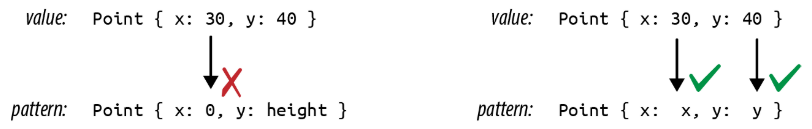
\includegraphics[width=0.8\textwidth]{../img/f10-6.png}
    \caption{结构体模式匹配}
    \label{f10-6}
\end{figure}

第二个分支可以匹配,因此输出将是\texttt{at (30m, 40m)}。

当匹配结构体时类似\texttt{Point \{ x: x, y: y \}}的模式非常常见,多余的名字也只会扰乱视觉,因此Rust为此支持一种缩写形式\texttt{Point \{x, y\}}。含义和之前相同,这个模式也会把点的\texttt{x}字段存储在新的局部变量\texttt{x}、把\texttt{y}字段存储在新的局部变量\texttt{y}。

即使有了缩写形式,如果我们要匹配一个很大的结构体但又只关心少数字段时还是会很麻烦:
\begin{minted}{Rust}
    match get_account(id) {
        ...
        Some(Account {
                name, language, // 我们关心的两个字段
                id: _, status: _, address: _, birthday: _, eye_color: _,
                pet: _, security_question: _, hashed_innermost_secret: _,
                is_adamantium_preferred_customer: _, }) =>
            language.show_custom_greeting(name),
    }
\end{minted}

为了避免这种情况,可以使用\texttt{..}告诉Rust你不关心其他的字段:
\begin{minted}{Rust}
    Some(Account { name, language, .. }) =>
        language.show_custom_greeting(name),
\end{minted}

\subsection{数字和切片模式}
数组模式匹配数组。它们被通常被用来过滤出某些特殊值,当数组的不同位置的含义不同时它们也会变得很有用。

例如,当把色相、饱和度、亮度(HSL)颜色值转换为红绿蓝(RGB)颜色值时,亮度为0的颜色就是黑、而亮度为满的颜色就是白。我们可以使用\texttt{match}表达式来简单地处理这些情况:
\begin{minted}{Rust}
    fn hsl_to_rgb(hsl: [u8; 3]) -> [u8; 3] {
        match hsl {
            [_, _, 0] => [0, 0, 0],
            [_, _, 255] => [255, 255, 255],
            ...
        }
    }
\end{minted}

切片模式与此类似,但和数组不同的是,切片的长度可以变化。因此切片模式并不只匹配值,还要匹配长度。切片模式中的\texttt{..}匹配任意数量的元素:
\begin{minted}{Rust}
    fn greet_people(names: &[&str]) {
        match names {
            [] => { println!("Hello, nobody.") },
            [a] => { println!("Hello, {}.", a) },
            [a, b] => { println!("Hello, {} and {}.", a, b) },
            [a, .., b] => { println!("Hello, everyone from {} to {}.", a, b) }
        }
    }
\end{minted}

\subsection{引用模式}
Rust模式支持两种和引用有关的特性。\texttt{ref}模式会借用被匹配的值,\texttt{\&}模式匹配引用。我们将首先介绍\texttt{ref}模式。

匹配一个非拷贝类型的值会移动这个值。继续上面的例子,下面的代码是无效的:
\begin{minted}{Rust}
    match account {
        Account { name, language, .. } => {
            ui.greet(&name, &language);
            ui.show_settings(&account); // error: borrow of moved value: `account`
        }
    }
\end{minted}

这里,字段\texttt{account.name}和\texttt{account.language}被移动进局部变量\texttt{name}和\texttt{language}中。\texttt{account}的其他部分被丢弃。这就是为什么我们不能再借用它的引用。

如果\texttt{name}和\texttt{language}都是可拷贝的值,Rust将会拷贝字段而不是移动它们,代码将没有问题。但假设它们就是\texttt{String},那我们该怎么办?

我们需要一种模式\emph{借用}被匹配的值而不是移动它们。\texttt{ref}关键字就是为此而生:
\begin{minted}{Rust}
    match account {
        Account { ref name, ref language, .. } => {
            ui.greet(name, language);
            ui.show_settings(&account); // ok
        }
    }
\end{minted}

现在局部变量\texttt{name}和\texttt{language}都是\texttt{account}中相应字段的引用。因此\texttt{account}只是被借用,并没有被消耗,所以继续用它调用方法也是OK的。

你可以使用\texttt{ref mut}来借用\texttt{mut}引用:
\begin{minted}{Rust}
    match line_result {
        Err(ref err) => log_error(err), // `err`是&Error(shared ref)
        Ok(ref mut line) => {           // `line`是&mut String(mut ref)
            trim_comments(line);        // 修改String
            handle(line);
        }
    }
\end{minted}

模式\texttt{Ok(ref mut line)}匹配任何成功值,并借用存储在里面的成功值的\texttt{mut}引用。

另一种相反的引用模式是\texttt{\&}模式。一个以\texttt{\&}开始的模式只能匹配引用:
\begin{minted}{Rust}
    match sphere.center() {
        &Point3d { x, y, z } => ...
    }
\end{minted}

在这个例子中,假设\texttt{sphere.center()}返回一个\texttt{sphere}的私有字段的引用,这在Rust中是很常见的。返回的值是一个\texttt{Point3d}的引用。如果中心在原点的话,\texttt{sphere.center()}会返回\texttt{\&Point3d \{ x: 0.0, y: 0.0, z: 0.0 \}}。

模式匹配按照\hyperref[f10-7]{图10-7}进行。

\begin{figure}[htbp]
    \centering
    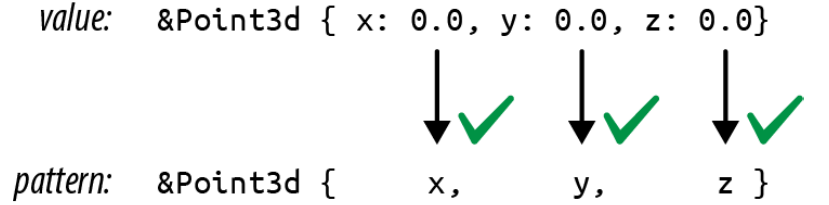
\includegraphics[width=0.8\textwidth]{../img/f10-7.png}
    \caption{引用的模式匹配}
    \label{f10-7}
\end{figure}

这里有一点诡异,因为Rust在这里解除了引用,也就是\texttt{*}运算符的功能。要记住模式和表达式天然是相反的。表达式\texttt{(x, y)}把两个值放入一个新的元组中,而模式\texttt{(x, y)}恰好相反:它匹配一个元组然后取出两个值。\texttt{\&}也是一样,在表达式里,\texttt{\&}创建一个引用;在模式里,\texttt{\&}匹配一个引用。

匹配一个引用遵循我们期望的所有规则:生命周期是强制的、你不能通过共享引用获取\texttt{mut}访问权限、你不能将值移动出引用,即使是\texttt{mut}引用。当我们匹配\texttt{\&Point3d \{ x, y, z \}}时,变量\texttt{x, y, z}都是坐标的拷贝,原本的\texttt{Point3d}值还是完整的。只有当这些字段都是拷贝类型才可以正常工作。如果我们想对结构体中一个不可拷贝的字段这么做,我们会遇到错误:
\begin{minted}{Rust}
    match friend.borrow_car() {
        Some(&Car { engine, .. }) => // error: can't move out of borrow
            ...
        None => {}
    }
\end{minted}

把一辆借来的车报废是不好的,Rust也不会允许这么做。你可以使用\texttt{ref}模式来借用一个引用,这样就不用拥有它:
\begin{minted}{Rust}
    Some(&Car { ref engine, .. }) => // ok, engine is a reference
\end{minted}

再来看另一个\texttt{\&}模式的例子。假设我们有一个迭代器\texttt{chars}迭代一个字符串里的所有字符,并且它有一个方法\texttt{chars.peek()}返回一个\texttt{Option<\&char>}:一个指向下一个字符的引用,如果有的话。(这类迭代器确实返回一个\texttt{Option<\&ItemType>},我们将在\hyperref[ch15]{第15章}中见到。)

一个程序可以使用\texttt{\&}来获得指向的字符:
\begin{minted}{Rust}
    match chars.peek() {
        Some(&c) => println!("coming up: {:?}", c),
        None => println!("end of chars"),
    }
\end{minted}

\subsection{匹配守卫}
有时一个匹配分支还有附加的条件必须要满足。假设我们在实现一个六边形空间内的棋子游戏,玩家只需要点击即可移动棋子。为了确认点击是有效的,我们可能要尝试类似这样的代码:
\begin{minted}{Rust}
    fn check_move(current_hex: Hex, click: Point) -> game::Result<Hex> {
        match point_to_hex(click) {
            None =>
                Err("That's not a game space."),
            Some(current_hex) => // 尝试匹配用户是不是点击了当前位置
                                 // (这样是错误的:原因如下)
                Err("You are already there! You must click somewhere else."),
            Some(other_hex) =>
                Ok(other_hex)
        }
    }
\end{minted}

这样是错误的,因为模式里的标识符会引入\emph{新的}变量。模式\texttt{Some(current\_hex)}会创建一个新的叫\texttt{current\_hex}的局部变量,然后遮蔽参数\texttt{current\_hex}。Rust会为这段代码报出好几个警告——尤其是,最后一个\texttt{match}分支不可达。一种修复这个问题的方法是简单地在分支中使用一个\texttt{if}表达式:
\begin{minted}{Rust}
    match point_to_hex(click) {
        None => Err("That's not a game space."),
        Some(hex) => {
            if hex == current_hex {
                Err("You are already there! You must click somewhere else")
            } else {
                Ok(hex)
            }
        }
    }
\end{minted}

不过Rust还提供了\emph{匹配守卫(match guard)}:模式和分支的\texttt{=>}词元中间的\texttt{if CONDITION}条件必须满足才能匹配:
\begin{minted}{Rust}
    match point_to_hex(click) {
        None => Err("That's not a game space."),
        Some(hex) if hex == current_hex =>
            Err("You are already there! You must click somewhere else"),
        Some(hex) => Ok(hex)
    }
\end{minted}

如果模式匹配,但条件不满足,那么将会继续匹配下一个分支。

\subsection{匹配多种可能}
竖线(|)可以用于在一个\texttt{match}分支中组合多个模式:
\begin{minted}{Rust}
    let at_end = match chars.peek() {
        Some(&'\r') | Some(&'\n') | None => true,
        _ => false,
    };
\end{minted}

在一个表达式中,|是位或运算符,但这里它的功能就像是普通表达式中的\texttt{||}。如果\texttt{chars.peek()}能匹配三个模式中的任意一个,\texttt{at\_end}就会被设为\texttt{true}。

使用\texttt{..=}来匹配范围内的值。范围模式包括起点和终点值,因此\texttt{'0' ..= '9'}匹配所有的ASCII数字:
\begin{minted}{Rust}
    match next_char {
        '0'..='9' => self.read_number(),
        'a'..='z' | 'A'..='Z' => self.read_word(),
        ' ' | '\t' | '\n' => self.skip_whitespace(),
        _ => self.handle_punctuation(),
    }
\end{minted}

Rust(目前)不允许在模式中使用尾开区间例如\texttt{0..100}。

\subsection{绑定和\texttt{@}模式}
最后,\texttt{x @ pattern}用给定的\texttt{pattern}来匹配,但匹配成功时它会创建单个变量\texttt{x}并把整个值移动或拷贝进去,而不是为匹配值的每一部分创建一个变量。例如,假设你有下面的代码:
\begin{minted}{Rust}
    match self.get_selection() {
        Shape::Rect(top_left, bottom_right) => {
            optimized_paint(&Shape::Rect(top_left, bottom_right))
        }
        other_shape => {
            paint_outline(other_shape.get_outline())
        }
    }    
\end{minted}
注意第一种情况会解包一个\texttt{Shape::Rect}值,然后在下一行中重新构建了一个新的\texttt{Shape::Rect}值。这可以被重写为\texttt{@}模式:
\begin{minted}{Rust}
    rect @ Shape::Rect(..) => {
        optimized_paint(&rect)
    }
\end{minted}

\texttt{@}模式和范围一起使用时也很有用:
\begin{minted}{Rust}
    match chars.next() {
        Some(digit @ '0'..='9') => read_number(digit, chars),
        ...
    },
\end{minted}

\subsection{模式可以用在哪里}
尽管模式最常用在\texttt{match}表达式中,但它们也能出现在一些其他地方,例如出现在标识符的位置。含义总是相同的:Rust使用模式匹配来分别取出值中的每一部分,而不是存储在单个变量中。

这意味着模式可以用于……
\begin{minted}{Rust}
    // ...把一个结构体解包为3个局部变量
    let Track { album, track_number, title, .. } = song;

    // ...解包一个元组类型的函数参数
    fn distance_to((x, y): (f64, f64)) -> f64 { .. }

    // ...迭代一个HashMap的键和值
    for (id, document) in &cache_map {
        println!("Document #{}: {}", id, document.title);
    }

    // ...自动解引用闭包的参数,
    // 当你想要一份拷贝时,其他代码可能会传给你一个引用,
    // 这时这种写法很方便。
    let sum = numbers.fold(0, |a, &num| a + num)
\end{minted}

这些写法都节省了两到三行重复的样本代码。其它语言中也有相同的概念:JavaScript中它被称为\emph{解构(destructuring)},而在Python中它被称为\emph{解包(unpacking)}。

注意这四个例子中,我们都使用了一定能匹配的模式。模式\texttt{Point3d \{ x, y, z \}}匹配\texttt{Point3d}类型的任意值,\footnote{译者注:此处应是作者写错了,应该是\texttt{Track}对应的例子。}\texttt{(x, y)}匹配任意的\texttt{(f64, f64)}类型的值,等等。在Rust中总是能匹配的模式是很特殊的,它们被称为\emph{不可反驳的模式(irrefutable pattern)},它们也是唯一能出现在这里展示的四种位置的模式(在\texttt{let}之后、在函数参数中、在\texttt{for}之后、在闭包的参数中)。

一个\emph{可反驳的模式(refutable pattern)}是那些可能不能匹配的模式,例如\texttt{Ok(x)},它不能匹配一个错误的Result,或者\texttt{'0' ..= '9'},它不能匹配字符\texttt{'Q'}。可反驳的模式可以用在\texttt{match}分支中,因为\texttt{match}就是为它们设计的:在\texttt{match}中如果匹配失败,那么接下来要怎么做很明显。而上面的四个例子中的位置,Rust不允许匹配失败。

可反驳的模式还可以用在\texttt{if let}和\texttt{while let}表达式中,它们可以用于……
\begin{minted}{Rust}
    // ...只有当是特定类型的枚举variant时才进行处理
    if let RoughTime::InTheFuture(_, _) = user.data_of_birth() {
        user.set_time_traveler(true);
    }

    // ...只有当查找成功时才运行代码
    if let Some(document) = cache_map.get(&id) {
        return send_cached_response(document);
    }

    // ...重复尝试执行操作直到它成功
    while let Err(err) = present_cheesy_anti_robot_task() {
        log_robot_attempt(err);
        // 让用户重试
    }

    // ...手动迭代器循环
    while let Some(_) = lines.peek() {
        read_paragraph(&mut lines);
    }
\end{minted}

有关这些表达式的细节,见\nameref{iflet}和\nameref{loop}。

\subsection{填充二叉树}\label{BinaryTree}
之前我们说过要展示如何实现一个\texttt{BinaryTree::add()}方法,它把一个节点添加到\\
\texttt{BinaryTree}中:
\begin{minted}{Rust}
    // 一个类型`T`的顺序集合
    enum BinaryTree<T> {
        Empty,
        NonEmpty(Box<TreeNode<T>>),
    }

    // 二叉树的一个节点
    struct TreeNode<T> {
        element: T,
        left: BinaryTree<T>,
        right: BinaryTree<T>,
    }
\end{minted}

现在你已经知道了编写这个方法所需的关于模式的知识。对二叉搜索树的解释已经超过了这本书的范围,但对于那些已经对这个话题很熟悉的读者,值得看一下在Rust中如何实现它。

\begin{minted}[linenos,numbersep=-1em]{Rust}
    impl<T: Ord> BinaryTree<T> {
        fn add(&mut self, value: T) {
            match *self {
                BinaryTree::Empty => {
                    *self = BinaryTree::NonEmpty(Box::new(TreeNode {
                        element: value,
                        left: BinaryTree::Empty,
                        right: BinaryTree::Empty,
                    }))
                }
                BinaryTree::NonEmpty(ref mut node) => {
                    if value <= node.element {
                        node.left.add(value);
                    } else {
                        node.right.add(value);
                    }
                }
            }
        }
    }    
\end{minted}

第1行告诉了Rust我们正在为有序类型的\texttt{BinaryTree}定义一个方法。这和我们之前为泛型结构体定义方法的语法完全相同,语法的解释见\nameref{method}一节。

如果现有的树\texttt{*self}是空的,那么就很简单。第5-9行把\texttt{Empty}树变成了一个\texttt{NonEmpty}的树。\texttt{Box::new()}的调用在堆上分配一个新的\texttt{TreeNode}。当运行完之后,树就有了一个元素,这个元素的左子树和右子树都是\texttt{Empty}。

如果\texttt{*self}不是空,第11行的模式就会匹配:
\begin{minted}{Rust}
    BinaryTree::NonEmpty(ref mut node) => {
\end{minted}

这个模式会借用一个\texttt{Box<TreeNode<T>>}的可变引用,因此我们可以访问并修改这个树节点中的数据。引用叫做\texttt{node},它的作用域是12到16行。因为这个节点中已经有一个元素了,所以需要递归调用\texttt{.add()}来给左子树或右子树的节点添加新元素。

新的方法可以像这样使用:
\begin{minted}{Rust}
    let mut tree = BinaryTree::Empty;
    tree.add("Mercury");
    tree.add("Venus");
    ...
\end{minted}

\section{宏观视图}

Rust的枚举对系统编程来说也许很新,但它们并不是一个新的概念。它有过很多学术性的名称,例如\emph{代数数据类型(algebraic data types)},它们在函数式编程语言中已经被使用了40多年。不知道为什么遵循C传统的语言中只有很少的语言有这种特性。可能只是因为对于一个编程语言的设计者来说,将variant、引用、可变性和内存安全融合在一起非常有挑战性。函数式语言不需要考虑可变性。C的\texttt{union}相反,有variant、指针和可变性——但它们是如此的不安全以至于即使在C中,它们也是最少用到的特性。Rust的借用检查器是使得在不妥协的情况下把这四者融合在一起变为可能的魔法。

程序就是数据处理的过程。一个小巧、快速、优雅的程序与一个充满缓慢、巨大的类型嵌套和虚拟方法调用的程序之间的区别可能就是是否把数据以正确的方式存储。

这正是枚举专注于解决的问题。它们是一种把数据以正确方式存储的设计工具。对于值可能是这样、也可能是那样、设置可能为空的情况,枚举在每一个维度上都比类层次结构要好:更快、更安全、更少的代码、更容易编写文档。

唯一的限制是灵活性。枚举的最终用户不能添加新的variant来扩展它。Variant只能通过修改枚举的定义来添加,而这么做的话,又会打破现有的代码。每一个单独匹配枚举的每个variant的\texttt{match}表达式都需要修改——需要添加一个新的分支来处理新的variant。在某些情况下,牺牲灵活性换取简洁性是明智之举。毕竟,像JSON这样的结构体预计不会改变。而在某些情况下,当枚举改变时修改所有使用的地方正是我们所期望的。例如,当一个编译器使用\texttt{enum}来表示语言中的不同运算符时,添加一个新的运算符\emph{应该}涉及到所有处理操作符的代码。

但有些时候也需要更多的灵活性。对于这些情况,Rust有trait,也就是我们下一章要讨论的话题。

    \include{ch11}
    \include{ch12}
    \include{ch13}
    \include{ch14}
    \include{ch15}
    \chapter{集合}\label{ch16}

\emph{We all behave like Maxwell’s demon. Organisms organize. In everyday experience lies the reason sober physicists across two centuries kept this cartoon fantasy alive. We sort the mail, build sand castles, solve jigsaw puzzles, separate wheat from chaff, rearrange chess pieces, collect stamps, alphabetize books, create symmetry, compose sonnets and sonatas, and put our rooms in order, and all this we do requires no great energy, as long as we can apply intelligence.}

\begin{flushright}
    ——James Gleick, The Information: A History, a Theory, a Flood
\end{flushright}

Rust标准库里包含几种\emph{集合(collection)},它们是在内存中存储数据的泛型类型。我们已经在本书的很多地方使用过集合,例如\texttt{Vec}和\texttt{HashMap}。在本章中,我们将详细介绍这两种类型的方法,以及其他六种标准集合。但在我们开始之前,让我们先讨论一下Rust的集合和其他语言中的集合的一些不同之处。

首先,移动和借用无处不在。Rust使用移动来避免深拷贝。这就是为什么\texttt{Vec<T>::push(item)}方法以值获取参数,而不是以引用。值会被移动进vector。\hyperref[ch04]{第4章}中的图展示了实践中的表现:在Rust中把一个\texttt{String}添加到\texttt{Vec<String>}中很快,因为Rust不需要拷贝字符串的字符数据,字符串的所有权归属也总是很清楚。

其次,当集合改变大小或者被修改的同时还有指向它们的数据的指针时,Rust不会有无效性错误——即悬垂指针。无效性错误是C++中另一种未定义行为的来源,即使在内存安全的语言中也可能导致\texttt{ConcurrentModificationException}。Rust借用检查器会在编译器检查出它们。

最后,Rust没有\texttt{null},因此我们将在其他语言中需要\texttt{null}的地方看到\texttt{Option}。

除了这些不同之外,Rust的集合可能正是你需要的。如果你是经验丰富的程序员并且时间不多,你可以跳过这部分,但不要跳过“\nameref{entry}”。

\section{概述}

\autoref{t16-1}展示了Rust的8种标准集合。它们都是泛型类型。

\begin{table}[htb]
    \centering
    \caption{标准集合总结}
    \label{t16-1}
    \begin{tabular}{p{0.2\textwidth}p{0.2\textwidth}lll}
        \hline
        \multirow{2}{*}{\textbf{集合}}  & \multirow{2}{*}{\textbf{说明}} & \multicolumn{3}{l}{\textbf{其他语言中的类似集合类型}} \\
        \cline{3-5}
         & & \textbf{C++} & \textbf{Java} & \textbf{Python} \\
        \hline
        
        \texttt{Vec<T>} & 可增长的数组  & \texttt{vector} & \texttt{ArrayList} & \texttt{list}  \\
        \rowcolor{tablecolor}
        \texttt{VecDeque<T>} & 双端队列(可增长环形缓冲区) & \texttt{deque} & \texttt{ArrayDeque} & \texttt{collections.deque} \\
        \texttt{LinkedList<T>} & 双向链表 & \texttt{list} & \texttt{LinkedList} & —— \\
        \rowcolor{tablecolor}
        \texttt{BinaryHeap<T> where T: Ord} & 大顶堆 & \texttt{priority\_queue} & \texttt{PriorityQueue} & \texttt{heapq} \\
        \texttt{HashMap<K, V> where K: Eq + Hash} & 键值哈希表 & \texttt{unordered\_map} & \texttt{HashMap} & \texttt{dict} \\
        \rowcolor{tablecolor}
        \texttt{BTreeMap<K, V> where K: Ord} & 有序键值表 & \texttt{map} & \texttt{TreeMap} & —— \\
        \texttt{HashSet<T> where T: Eq + Hash} & 基于哈希的无序集合 & \texttt{unordered\_set} & \texttt{HashSet} & \texttt{set} \\
        \rowcolor{tablecolor}
        \texttt{BTreeSet<T> where T: Ord} & 有序集合 & \texttt{set} & \texttt{TreeSet} & —— \\
    \end{tabular}
\end{table}

\texttt{Vec<T>}、\texttt{HashMap<K, V>}、\texttt{HashSet<T>}是最常用的集合类型。其他的集合都有适用的场景。这一章将轮流讨论每一个集合类型:

\codeentry{Vec<T>}
\hangparagraph{一个可增长的、在堆上分配的、\texttt{T}类值的数组。本章中大约一半的篇幅专门介绍\texttt{Vec}和它的常用方法。}

\codeentry{VecDeque<T>}
\hangparagraph{类似于\texttt{Vec<T>},但是用作先进先出队列会更好。它支持高效地在首部和尾部添加或移除元素,但这种能力的代价是其他操作会稍微慢一点。}

\codeentry{BinaryHeap<T>}
\hangparagraph{一个优先队列。\texttt{BinaryHeap}中的值按照一定结构组织,因此总是可以高效地找到和移除最大值。}

\codeentry{HashMap<K, V>}
\hangparagraph{一个键值对的表。通过键查找值很快速。表中的条目以任意顺序存储。}

\codeentry{BTreeMap<K, V>}
\hangparagraph{类似于\texttt{HashMap<K, V>},但按键的顺序保持条目有序。一个\texttt{BTreeMap<String, i32>}按照\texttt{String}的比较顺序存储条目。除非你需要条目保持有序,否则\texttt{HashMap}会更快。}

\codeentry{HashSet<T>}
\hangparagraph{类型\texttt{T}的值的集合。添加和删除元素都很快,查询一个值是否在集合中也很快。}

\codeentry{BTreeSet<T>}
\hangparagraph{类似于\texttt{HashSet<T>},但保持元素有序。同样,除非你想要数据保持有序,否则\texttt{HashSet}会更快。}

因为\texttt{LinkedList}很少使用(并且在大多数情况下都有更好的替代,无论是性能还是接口),因此我们不会在这里介绍它。

\section{\texttt{Vec<T>}}

我们假设你对\texttt{Vec}已经有了一定了解,因为我们在本书的很多地方都已经使用过它。简要的介绍见“\nameref{vector}”。这里我们只会描述它的方法以及深入它的内部工作原理。

最简单的创建vector的方式是使用\texttt{vec!}宏:
\begin{minted}{Rust}
    // 创建一个空的vector
    let mut numbers: Vec<i32> = vec![];

    // 用给定的内容创建一个vector
    let words = vec!["step", "on", "no", "pets"];
    let mut buffer = vec![0u8; 1024];   // 1024个0字节
\end{minted}

正如我们在“\hyperref[ch04]{第4章}”所述,vector有三个字段:长度、容量、和一个指向堆上分配的缓冲区的指针。\autoref{f16-1}展示了上面的vector在内存中的视图。空vector,\texttt{numbers},初始长度为0。在它添加第一个元素之前不会有堆内存被分配。

\begin{figure}[htbp]
    \centering
    \includegraphics[width=0.9\textwidth]{../img/f16-1.png}
    \caption{vector的内存布局:words的每个元素是一个由指针和长度组成的\&str值}
    \label{f16-1}
\end{figure}

类似于所有集合,\texttt{Vec}实现了\texttt{std::iter::FromIterator},因此你可以对任何迭代器调用\texttt{.collect()}方法来创建一个vector,正如“\nameref{BuildColl}”中所述:
\begin{minted}{Rust}
    // 将一个其他集合转换成vector
    let my_vec = my_set.into_iter().collect::<Vec<String>>();
\end{minted}

\subsection{访问元素}
通过索引访问数组、切片或vector的元素非常直观:
\begin{minted}{Rust}
    // 获取一个元素的引用
    let first_line = &lines[0];

    // 获取一个元素的拷贝 
    let fifth_number = numbers[4];          // 需要Copy
    let second_number = lines[1].clone();   // 需要Clone

    // 获取一个切片的引用
    let my_ref = &buffer[4..12];

    // 获取一个切片的拷贝
    let my_copy = buffer[4..12].to_vec();   // 需要Clone
\end{minted}

当索引越界时所有这些方式都会panic。

Rust对数字类型很挑剔,vector也不例外。vector的长度和索引都是\texttt{usize}类型。尝试使用\texttt{u32}、\texttt{u64}、\texttt{isize}作为vector的索引会导致错误。必要时你可以使用\texttt{n as usize}来转换,见“\nameref{cast}”。

有几种方法提供了便捷地访问vector或切片的特定元素的方法(注意所有的切片方法都能用于数组和vector):
\codeentry{slice.first()}
\hangparagraph{返回\texttt{slice}的第一个元素的引用。返回类型是\texttt{Option<\&T>},因此如果\texttt{slice}为空时返回值为\texttt{None},不为空时返回值为\texttt{Some(\&slice[0])}:}
\begin{minted}{Rust}
    if let Some(item) = v.first() {
        println!("We got one! {}", item);
    }
\end{minted}

\codeentry{slice.last()}
\hangparagraph{和上边相似,不过返回最有一个元素的引用。}

\codeentry{slice.get(index)}
\hangparagraph{返回\texttt{slice[index]}的引用,如果存在的话。如果\texttt{slice}的元素数量小于\texttt{index+1},那么返回\texttt{None}:}
\begin{minted}{Rust}
    let slice = [0, 1, 2, 3];
    assert_eq!(slice.get(2), Some(&2));
    assert_eq!(slice.get(4), None);
\end{minted}

\codeentry{slice.first\_mut(), slice.last\_mut(), slice.get\_mut(index)}
\hangparagraph{与上面的类似,不过借用\texttt{mut}引用:}
\begin{minted}{Rust}
    let mut slice = [0, 1, 2, 3];
    {
        let last = slice.last_mut().unwrap();   // 最后一个元素类型:&mut i32
        assert_eq!(*last, 3);
        *last = 100;
    }
\end{minted}

因为以值返回\texttt{T}意味着移动它,因此访问元素的方法通常返回元素的引用。

一个例外是\texttt{.to\_vec()}方法,它获取拷贝:

\codeentry{slice.to\_vec()}
\hangparagraph{克隆整个切片,返回一个新的vector:}
\begin{minted}{Rust}
    let v = [1, 2, 3, 4, 5, 6, 7, 8, 9];
    assert_eq!(v.to_vec(),
               vec![1, 2, 3, 4, 5, 6, 7, 8, 9]);
    assert_eq!(v[0..6].to_vec(),
               vec![1, 2, 3, 4, 5, 6]);
\end{minted}
\hangparagraph{只有当元素可以拷贝时这个方法才可用,即\texttt{where T: Clone}}

\subsection{迭代}\label{Iteration}
vector和切片可以以值或者以引用迭代,遵循“\nameref{IntoIter}”中介绍的模式:
\begin{itemize}
    \item 迭代\texttt{Vec<T>}会产生\texttt{T}类型的item。元素被逐个移出vector消耗掉。
    \item 迭代\texttt{\&[T; N], \&[T], \&Vec<T>}——即数组、切片或vector的引用——会产生\texttt{\&T}类型的item,每一个item指向一个元素,不会移动元素。
    \item 迭代\texttt{\&mut [T; N], \&mut [T], \&mut Vec<T>}产生\texttt{\&mut T}类型的item。
\end{itemize}

数组、切片和vector还有\texttt{.iter()}和\texttt{.iter\_mut()}方法(见“\nameref{IterMethod}”)创建产生元素的引用的迭代器。

我们将在“\nameref{split}”中介绍一些更有趣的迭代切片的方法。

\subsection{增长和缩减vector}
数组、切片或vector的\emph{长度(length)}是它包含的元素的数量:

\codeentry{slice.len()}
\hangparagraph{返回一个\texttt{slice}的长度,类型为\texttt{usize}。}

\codeentry{slice.is\_empty()}
\hangparagraph{当\texttt{slice}不包含元素时为真(即\texttt{slice.len() == 0})。}

本节剩余的方法都是关于增长和缩减vector。它们不能用于数组和切片,因为它们一旦被创建之后就不能改变大小。

vector的所有元素都存储在一个在堆上分配的连续内存块中。vector的\emph{容量(capacity)}是指当前的内存块中最多能存储的元素数量。\texttt{Vec}通常会替你管理容量,当需要增长时它会自动分配更大的缓冲区并把元素都移动过去。还有一些显式管理容量的方法:

\codeentry{Vec::with\_capacity(n)}
\hangparagraph{创建一个容量为\texttt{n}的新的空vector。}

\codeentry{vec.capacity()}
\hangparagraph{返回\texttt{vec}的容量,类型是\texttt{usize}。\texttt{vec.capacity() >= vec.len()}总是为真。}

\codeentry{vec.reserve(n)}
\hangparagraph{保证vector的剩余空间至少还能再存储\texttt{n}个或更多元素:即\texttt{vec.capacity()}至少是\texttt{vec.len() + n}。如果已经有足够的空间,它不做任何事。否则,它会分配一个更大的缓冲区并且把vector的内容移动过去。}

\codeentry{vec.reserve\_exact(n)}
\hangparagraph{类似于\texttt{vec.reserve(n)},但告诉\texttt{vec}不要为未来的增长分配额外的空间。调用它之后,\texttt{vec.capacity()}等于\texttt{vec.len() + n}。}

\codeentry{vec.shrink\_to\_fit()}
\hangparagraph{当\texttt{vec.capacity()}大于\texttt{vec.len()}时尝试释放额外的内存。}

\texttt{Vec<T>}有很多添加或移除元素的方法,同时改变vector的长度。所有这些方法都以\texttt{mut}引用获取\texttt{self}参数。

下面这两个方法在vector的末尾添加或移除一个元素:

\codeentry{vec.push(value)}
\hangparagraph{把\texttt{value}添加到\texttt{vec}的末尾。}

\codeentry{vec.pop()}
\hangparagraph{移除并返回最后一个元素。返回类型是\texttt{Option<T>}。当vector已经为空时返回\texttt{None},否则返回\texttt{Some(x)}。}

注意\texttt{.push()}以值而不是以引用获取参数。类似的,\texttt{.pop()}返回被弹出的值,而不是引用。本节中剩余的大部分方法也是这样。它们从vector移出或移进值。

这两个方法向vector中添加值或者从vector中移出值:
\codeentry{vec.insert(index, value)}
\hangparagraph{在\texttt{vec[index]}处插入给定的\texttt{value},把\texttt{vec[index..]}中的值都向后移动一个位置来腾出空间。如果\texttt{index > vec.len()}会panic。}

\codeentry{vec.remove(index)}
\hangparagraph{移除并返回\texttt{vec[index]},把\texttt{vec[index+1..]}中的值向左移动一个位置来消除缝隙。}

\texttt{.insert()}和\texttt{.remove()}都很慢,因为有很多元素需要移动。

有四个方法可以将vector的长度调整为指定值:

\codeentry{vec.resize(new\_len, value)}
\hangparagraph{将\texttt{vec}的长度设为\texttt{new\_len}。如果这会增大\texttt{vec}的长度,将会用\texttt{value}的拷贝填充新空间。元素的类型必须实现了\texttt{Clone} trait。}

\codeentry{vec.resize\_with(new\_len, closure)}
\hangparagraph{类似于\texttt{vec.resize},但调用闭包来构造每一个新元素。它可以用于元素没有实现\texttt{Clone}的vector。}

\codeentry{vec.truncate(new\_len)}
\hangparagraph{将\texttt{vec}的长度缩减到\texttt{new\_len},丢弃\texttt{vec[new\_len..]}范围内的所有元素。如果\texttt{vec.len()}小于等于\texttt{new\_len},那么什么也不做。}

\codeentry{vec.clear()}
\hangparagraph{删除\texttt{vec}的所有元素。等价于\texttt{vec.truncate(0)}。}

有四个方法可以一次添加或移除很多元素:

\codeentry{vec.extend(iterable)}
\hangparagraph{将\texttt{iterable}的所有item按顺序添加到\texttt{vec}的末尾。它类似于多值版本的\texttt{.push()}。\texttt{iterable}参数可以是任何实现了\texttt{IntoIterator<Item=T>}。}

\hangparagraph{这个方法如此有用以至于有一个专门的trait \texttt{Extend},所有的标准集合都实现了它。不幸的是,这导致\texttt{rustdoc}将\texttt{.extend()}和其他trait的方法放在生成的HTML底部的一堆方法中,因此当你需要它时很难找到它。你必须记住它!更多内容见“\nameref{extend}”。}

\codeentry{vec.split\_off(index)}
\hangparagraph{类似于\texttt{vec.truncate(index)},除了它返回一个\texttt{Vec<T>}包含\texttt{vec}尾部被移除的元素。它类似于\texttt{.pop()}的多值版本。}

\codeentry{vec.append(\&mut vec2)}
\hangparagraph{这会把\texttt{vec2}的所有元素移动进\texttt{vec},其中\texttt{vec2}是另一个\texttt{Vec<T>}类型的vector。调用之后,\texttt{vec2}变为空。}

\hangparagraph{这类似于\texttt{vec.extend(vec2)},除了调用之后\texttt{vec2}仍然存在,并且容量不变。}

\codeentry{vec.drain(range)}
\hangparagraph{这会从\texttt{vec}中移除范围\texttt{vec[range]},并返回一个迭代被移除元素的迭代器,其中\texttt{range}是一个范围值,例如\texttt{..}或\texttt{0..4}。}

还有一些选择性移除vector元素的古怪方法:
\codeentry{vec.retain(test)}
\hangparagraph{移除所有没有通过给定测试的方法。\texttt{test}参数是一个实现了\texttt{FnMut(\&T) -> bool}的函数或闭包。对于\texttt{vec}的每一个元素,它会调用\texttt{test(\&element)},如果返回\texttt{false},元素将会被移出vector然后丢弃。}

\hangparagraph{不考虑性能的话,这类似于:}
\begin{minted}{Rust}
    vec = vec.into_iter().filter(test).collect();
\end{minted}

\codeentry{vec.dedup()}
\hangparagraph{丢弃相邻的重复元素。它类似于Unix的\texttt{uniq} shell工具。它会扫描\texttt{vec}中寻找相邻的重复元素,然后丢弃掉多余的重复值,只留下一个:}
\begin{minted}{Rust}
    let mut byte_vec = b"Missssssissippi".to_vec();
    byte_vec.dedup();
    assert_eq!(&byte_vec, b"Misisipi");
\end{minted}
\hangparagraph{注意最后的输出中仍然有两个\texttt{'s'}字符。这个方法只移除\emph{相邻的(adjacent)}重复值。为了移除所有的重复值,你有三种选择:调用\texttt{.dedup()}之前先排序vector,将数据移动到一个“\nameref{set}”,或者(为了保持元素原本的顺序)使用这个\texttt{.retain()}技巧:}
\begin{minted}{Rust}
    let mut byte_vec = b"Missssssissippi".to_vec();

    let mut seen = HashSet::new();
    byte_vec.retain(|r| seen.insert(*r));

    assert_eq!(&byte_vec, b"Misp");
\end{minted}
\hangparagraph{这段代码的原理是当集合中已经包含要插入的item时\texttt{.insert()}会返回\texttt{false}。}

\codeentry{vec.dedup\_by(same)}
\hangparagraph{类似于\texttt{vec.dedup()},但它使用函数或者闭包\texttt{same(\&mut elem1, \&mut elem2)},而不是\texttt{==}运算符,来检查两个相邻元素是否被认为相等。}

\codeentry{vec.dedup\_by\_key(key)}
\hangparagraph{类似于\texttt{vec.dedup()},但当\texttt{key(\&mut elem1) == key(\&mut elem2)}时它认为两个元素相等。}

\hangparagraph{例如,如果\texttt{errors}是一个\texttt{Vec<Box<dyn Error>>},你可以写:}
\begin{minted}{Rust}
    // 移除消息重复的错误。
    errors.dedup_by_key(|err| err.to_string());
\end{minted}

这一节介绍的所有方法中,只有\texttt{.resize()}可能会拷贝值。其他的通过移动值来工作。

\subsection{连接}
两个方法可以用于\emph{数组的数组(array of array)},即元素类型是数组、切片、vector的数组、切片、vector:

\codeentry{slices.concat()}
\hangparagraph{返回一个所有切片连接成的vector:}
\begin{minted}{Rust}
    assert_eq!([[1, 2], [3, 4], [5, 6]].concat(),
               vec![1, 2, 3, 4, 5, 6]);
\end{minted}

\codeentry{slices.join(\&separator)}
\hangparagraph{同上,除了会在切片之间插入\texttt{separator}的拷贝:}
\begin{minted}{Rust}
    assert_eq!([[1, 2], [3, 4], [5, 6]].join(&0),
               vec![1, 2, 0, 3, 4, 0, 5, 6]);
\end{minted}

\subsection{切分}\label{split}
很容易一次获得数组、切片、vector中的很多元素的非\texttt{mut}引用:
\begin{minted}{Rust}
    let v = vec![0, 1, 2, 3];
    let a = &v[i];
    let b = &v[j];

    let mid = v.len() / 2;
    let front_half = &v[..mid];
    let back_half = &v[mid..];
\end{minted}

但一次获得多个\texttt{mut}引用不是这么容易:
\begin{minted}{Rust}
    let mut v = vec![0, 1, 2, 3];
    let a = &mut v[i];
    let b = &mut v[j];  // error: 不能同时借用`v`的
                        // 多个可变引用。

    *a = 6;             // 引用`a`和`b`在这里使用了,
    *b = 7;             // 因此它们的生命周期一定会重叠。
\end{minted}

Rust禁止这样,因为如果\texttt{i == j},那么\texttt{a}和\texttt{b}将是同一个整数的两个\texttt{mut}引用,这违背了Rust的安全性的规则。(见“\nameref{ShareVSMut}”)。

Rust有几个方法可以一次借用数组、切片、vector的两个或更多元素的\texttt{mut}引用。和上面的代码不同,这些方法是安全的,因为它们从设计上保证了只会把数组分割成\emph{非重叠(nonoverlapping)区域}。这些方法也可以用于非\texttt{mut}切片,因此它们有\texttt{mut}和非\texttt{mut}版本。

\begin{figure}[htbp]
    \centering
    \includegraphics[width=0.9\textwidth]{../img/f16-2.png}
    \caption{分割方法展示(注意:\texttt{slice.split()}输出中的小矩形是空的切片,因为两侧都是分隔符,\texttt{rsplitn}的输出是按照从后往前的顺序,这一点和其他的不同。}
    \label{f16-2}
\end{figure}

这些方法中没有一个会直接修改数组、切片或vector;它们都返回部分数据的引用:
\codeentry{slice.iter(), slice.iter\_mut()}
\hangparagraph{产生\texttt{slice}的每个元素的引用。我们在“\nameref{Iteration}”中已经介绍过它们。}

\codeentry{slice.split\_at(index), slice.split\_at\_mut(index)}
\hangparagraph{将一个切片划分为两个,返回一个pair。\texttt{slice.split\_at(index)}等价于\texttt{(\&slice[..index], \\
\&slice[index..])}。如果\texttt{index}越界会panic。}

\codeentry{slice.split\_first(), slice.split\_first\_mut()}
\hangparagraph{也返回一个pair:第一个元素的引用(\texttt{slice[0]})和其余所有元素的切片引用(\texttt{slice[1..]})。}

\hangparagraph{\texttt{.spilt\_first()}的返回值类型是\texttt{Option<(\&T, \&[T])>};如果\texttt{slice}为空,返回\texttt{None}。}

\codeentry{slice.split\_last(), slice.split\_last\_mut()}
\hangparagraph{类似上一个,不过划分出最后一个元素而不是第一个。}

\hangparagraph{\texttt{.split\_last()}的返回类型是\texttt{Option<(\&T, \&[T])>}。}

\codeentry{slice.split(is\_sep), slice.split\_mut(is\_sep)}
\hangparagraph{将\texttt{slice}切分成一个或更多子切片,使用函数或闭包\texttt{is\_sep}来判断在哪里切分。它们返回一个迭代子切片的迭代器。}

\hangparagraph{当你消耗迭代器时,它会对切片中的每个元素调用\texttt{is\_sep(\&element)}。如果\texttt{is\_sep(\&element)}返回\texttt{true},那么这个元素就是一个分隔符。分隔符不包含在任何输出的字切片中。}

\hangparagraph{输出总是包含至少一个子切片,每有一个分隔符就加一个子切片。如果有相邻的分隔符或者\texttt{slice}的两端是分隔符都会产生空的子切片。}

\codeentry{slice.rsplit(is\_sep), slice.rsplit\_mut(is\_sep)}
\hangparagraph{类似于\texttt{slice}和\texttt{slice\_mut},但从最后一个切片开始。}

\codeentry{slice.splitn(n, is\_sep), slice.splitn\_mut(n, is\_sep)}
\hangparagraph{类似上面的方法,不过最多产生\texttt{n}个子切片。当发现了前\texttt{n-1}个切片之后就不会再调用\texttt{is\_sep}。最后一个字切片将包含剩余的所有元素。}

\codeentry{slice.rsplitn(n, is\_sep), slice.rsplitn\_mut(n, is\_sep)}
\hangparagraph{类似于\texttt{.splitn()}和\texttt{.splitn\_mut()},除了反向扫描切片。就是说,这个方法会在切片中\emph{最后}\texttt{n-1}个分隔符处切分,而不是前\texttt{n-1}个,并且从尾部开始产生子切片。}

\codeentry{slice.chunks(n), slice.chunks\_mut(n)}
\hangparagraph{返回一个产生长度为\texttt{n}的非重叠子切片的迭代器。如果\texttt{n}不能整除\texttt{slice.len()},最后一个块的元素数量将小于\texttt{n}。}

\codeentry{slice.rchunks(n), slick.rchunks\_mut(n)}
\hangparagraph{类似于\texttt{slice.chunks()}和\texttt{slice.chunks\_mut()},但是从切片的尾部开始。}

\codeentry{slice.chunks\_exact(n), slice.chunks\_exact\_mut(n)}
\hangparagraph{返回一个产生长度为\texttt{n}的非重叠子切片的迭代器。如果\texttt{n}不能整除\texttt{slice.len()},最后一个块(元素数量小于\texttt{n})可以通过结果的\texttt{remainder()}方法获得。}

\codeentry{slice.rchunks\_exact(n), slice.rchunks\_exact\_mut(n)}
\hangparagraph{类似于\texttt{slice.chunks\_exact}和\texttt{slice.chunks\_exact\_mut},但从切片的尾部开始。}

还有一些其他迭代子切片的方法:
\codeentry{slice.windows(n)}
\hangparagraph{返回一个效果类似于“滑动窗口”的迭代器。它产生\texttt{slice}中相邻的\texttt{n}个元素的子切片。第一个产生的值是\texttt{\&slice[0..n]},第二个是\texttt{\&slice[1..n+1]},以此类推。}

\hangparagraph{如果\texttt{n}大于\texttt{slice}的长度,将不会产生切片。如果\texttt{n}是0,这个方法会panic。}

\hangparagraph{例如,如果\texttt{days.len() == 31},那么我们可以调用\texttt{days.windows(7)}产生\texttt{days}中所有7天的区间。}

\hangparagraph{在探索数据列的变化趋势时一个大小为2的滑动窗口会很有用:}
\begin{minted}{Rust}
    let changes = daily_high_temperatures
                      .windows(2)           // 获得相邻天的温度
                      .map(|w| w[1] - w[0]) // 温度改变了多少
                      .collect::<Vec<_>>();
\end{minted}
\hangparagraph{因为子切片是重叠的,所以这个方法没有返回\texttt{mut}引用的版本。}

\subsection{交换}
有一些交换切片内容的便捷方法:

\codeentry{slice.swap(i, j)}
\hangparagraph{交换元素\texttt{slice[i]}和\texttt{slice[j]}。}

\codeentry{slice\_a.swap(\&mut slice\_b)}
\hangparagraph{交换\texttt{slice\_a}和\texttt{slice\_b}的全部内容。\texttt{slice\_a}和\texttt{slice\_b}长度必须相同。}

vector有一个高效地移除任何元素的方法:

\codeentry{vec.swap\_remove(i)}
\hangparagraph{移除并返回\texttt{vec[i]}。这类似于\texttt{vec.remove(i)},除了它不是吧剩余的元素往前移动来消除间隙,而是把\texttt{vec}的最后一个元素移动到间隙。当你不关心vector中元素的顺序时这很有用。}

\subsection{排序和搜索}
切片提供了三个用于排序的方法:

\codeentry{slice.sort()}
\hangparagraph{按增序排序元素。只有当元素类型实现了\texttt{Ord},这个方法才可用。}

\codeentry{slice.sort\_by(cmp)}
\hangparagraph{使用函数或闭包\texttt{cmp}指定顺序来排序\texttt{slice}的元素。\texttt{cmp}必须实现了\texttt{Fn(\&T, \&T) -> std::cmp::Ordering}。}

\hangparagraph{手动实现\texttt{cmp}很麻烦,除非你用\texttt{.cmp}方法:}
\begin{minted}{Rust}
    students.sort_by(|a, b| a.last_name.cmp(&b.last_name));
\end{minted}
\hangparagraph{如果要先比较一个字段,再比较第二个字段,可以直接比较元组:}
\begin{minted}{Rust}
    students.sort_by(|a, b| {
        let a_key = (&a.last_name, &a.first_name);
        let b_key = (&b.last_name, &b.first_name);
        a_key.cmp(&b_key)
    });
\end{minted}

\codeentry{slice.sort\_by\_key(key)}
\hangparagraph{以给定的函数或闭包\texttt{key}作为排序键将\texttt{slice}的元素按照增序排序。\texttt{key}的类型必须实现了\texttt{Fn(\&T) -> K where K: Ord}}。
\hangparagraph{当\texttt{T}包含一个或更多有序字段时这很有用,因为它可以按照多种方式排序:}
\begin{minted}{Rust}
    // 按照平均绩点排序,低的靠前
    students.sort_by_key(|s| s.grade_point_average());
\end{minted}
\hangparagraph{注意这些排序键在排序过程中并不会被缓存,因此\texttt{key}函数可能会被调用超过\texttt{n}次。}

\hangparagraph{出于技术上的原因,\texttt{key(element)}不能返回任何从元素借用的引用。这样不能工作:}
\begin{minted}{Rust}
    students.sort_by_key(|s| &s.last_name); // 错误:无法推断生命周期
\end{minted}
\hangparagraph{Rust无法查明生命周期。但在这种情况下,可以调用\texttt{.sort\_by()}作为替代。}

这三种方法都是稳定性排序。

为了实现反向排序,你可以使用\texttt{sort\_by},然后在\texttt{cmp}闭包中交换两个参数。将参数写为\texttt{|b, a|}而不是\texttt{|a, b|}可以高效地产生相反的顺序。或者你可以在排序之后调用\texttt{.reverse()}方法:

\codeentry{slice.reverse()}
\hangparagraph{反转一个切片。}

一旦一个切片被排过序,它就可以被高效地搜索:
\codeentry{slice.binary\_search(\&value), slice.binary\_search\_by(\&value, cmp), slice.binary\_search\_by\_key(\&value, key)}
\hangparagraph{这些方法都在有序的\texttt{slice}中搜索\texttt{value}。注意\texttt{value}是以引用传递。}

\hangparagraph{这些方法的返回类型都是\texttt{Result<usize, usize>}。如果\texttt{slice[index]}在指定的排序顺序下等于\texttt{value}它们会返回\texttt{Ok(index)}。如果没有这样的元素,它们会返回\texttt{Err(insertion\_point)},在\texttt{insertion\_point}处插入\texttt{value}将保持有序。}

当然,二分搜索只在切片在指定的顺序下有序时才能工作。否则,结果将是任意值——garbage in, garbage out。

因为\texttt{f32}和\texttt{f64}有NaN值,它们没有实现\texttt{Ord},因此不能被直接用作排序或二分搜索的键。为了得到可以用于浮点数的类似方法,使用\texttt{ord\_subset} crate。

还有一个在无序vector中搜索元素的方法:

\codeentry{slice.contains(\&value)}
\hangparagraph{如果\texttt{slice}中有任何元素等于\texttt{value}时返回\texttt{true}。它简单地检查切片的每个元素,直到找到要查找的值。还有,\texttt{value}也是以引用传递。}

为了查找一个切片中某一个值的位置,类似于JavaScript中的\texttt{array.indexOf(value)},使用迭代器:
\begin{minted}{Rust}
    slice.iter().position(|x| *x == value)
\end{minted}
这会返回\texttt{Option<usize>}。

\subsection{比较切片}
如果类型\texttt{T}支持\texttt{==}和\texttt{!=}运算符(\texttt{PartialEq} trait,见“\nameref{equal}”),那么数组\texttt{[T; N]}、切片\texttt{[T]}、vector \texttt{Vec<T>}也支持这些运算符。当两个切片的长度和相应的元素都相等时两个切片才相等。数组和vector也是一样。

如果\texttt{T}支持运算符\texttt{<}、\texttt{<=}、\texttt{>}、\texttt{>=}(\texttt{PartialOrd} trait,见“\nameref{cmp}”),那么\texttt{T}的数组、切片和vector也支持。切片的比较按照字典序进行。

有两个便捷的方法进行常用的切片比较:

\codeentry{slice.starts\_with(other)}
\hangparagraph{如果\texttt{slice}起始的值序列等于\texttt{other}的元素则返回\texttt{true}:}
\begin{minted}{Rust}
    assert_eq!([1, 2, 3, 4].starts_width(&[1, 2]), true);
    assert_eq!([1, 2, 3, 4].starts_width(&[2, 3]), false);
\end{minted}

\codeentry{slice.ends\_with(other)}
\hangparagraph{和上边类似但检查\texttt{slice}的末尾:}
\begin{minted}{Rust}
    assert_eq!([1, 2, 3, 4].ends_with(&[3, 4]), true);
\end{minted}

\subsection{随机元素}
Rust的标准库中并不包含随机数。\texttt{rand} crate提供了它们,还提供了两个方法从数组、切片、vector中获取随机元素:

\codeentry{slice.choose(\&mut rng)}
\hangparagraph{返回切片中随机一个元素的引用。类似于\texttt{slice.first()}和\texttt{slice.last()},除了它返回一个\texttt{Option<\&T>},如果切片为空,返回值为\texttt{None}。}

\codeentry{slice.shuffle(\&mut rng)}
\hangparagraph{随机打乱切片中的元素的顺序。切片必须以\texttt{mut}引用传递。}

这些是\texttt{rand::Rng} trait的方法,因此为了调用它们你需要一个\texttt{Rng},它是一个随机数生成器。幸运的是,可以调用\texttt{rand::thread\_rng()}来获得一个。要想打乱vector \texttt{my\_vec},你可以写:
\begin{minted}{Rust}
    use rand::seq::SliceRandom;
    use rand::thread_rng;

    my_vec.shuffle(&mut thread_rng());
\end{minted}

\subsection{Rust排除了无效性错误}
大多数主流编程语言都有集合和迭代器,而且都有这个规则的变体:不要在遍历集合的同时修改它。例如,Python中vecotr等价的是list:
\begin{minted}{Rust}
    my_list = [1, 3, 5, 7, 9]
\end{minted}

假设我们想移除\texttt{my\_list}中大于4的元素;
\begin{minted}{python}
    for index, val in enumerate(my_list):
        if val > 4:
            del my_list[index]  # bug: 在迭代的同时修改
    
    print(my_list)
\end{minted}
(Python中的\texttt{enumerate}函数等价于Rust中的\texttt{.enumerate()}方法,见“\nameref{enumerate}”。)

这个程序令人惊讶地打印出\texttt{[1, 3, 7]}。但7比4大,为什么它没被移除?这就是无效性错误:程序在迭代数据的同时修改它,将迭代器\emph{无效化(invalidate)}。在Java中,结果可能是一个异常;在C++中是未定义行为。而在Python中,这个行为是有定义的,虽然不太直观:
迭代器会跳过一个元素。\texttt{val}永远不会是\texttt{7}。

让我们尝试在Rust中复现这个bug:
\begin{minted}{Rust}
    fn main() {
        let mut my_vec = vec![1, 3, 5, 7, 9];
        
        for (index, &val) in my_vec.iter().enumerate() {
            if val > 4 {
                my_vec.remove(index);   // error: can't borrow `my_vec` as mutable
            }
        }
        println!("{:?}", my_vec);
    }
\end{minted}

Rust自然会在编译期拒绝这个程序。当我们调用\texttt{my\_vec.iter()}时,它借用了vector的一个共享(非\texttt{mut})引用。引用的生命周期和迭代器一样长,也就是直到\texttt{for}循环的结尾。我们不能在有非\texttt{mut}引用存在时调用\texttt{my\_vec.remove(index)}修改vector。

编译器能指出这个错误非常好,但当然,你仍然需要一种方法来得到期望的行为!这里最简单的修复方法是:
\begin{minted}{Rust}
    my_vec.retain(|&val| val <= 4);
\end{minted}

或者,你可以采用在Python或其他任何语言中也可以实现的方法:使用\texttt{filter}来创建一个新的vector。

\section{\texttt{VecDeque<T>}}

\texttt{Vec}只支持在尾部高效地添加和删除元素。当一个程序需要存储“排队”的值时,\texttt{Vec}会变得很慢。

Rust的集合\texttt{std::collections::VecDeque<T>}是一个\emph{双端队列(deque)}(读作“deck”)。它支持在头部和尾部高效地添加和移除元素:

\codeentry{deque.push\_front(value)}
\hangparagraph{在队列的头部添加一个值。}

\codeentry{deque.push\_back(value)}
\hangparagraph{在尾部添加一个值。(这个方法比\texttt{.push\_front()}用得更多,因为队列的通常用法是从尾部添加并从头部移除,就像人在排队一样。}

\codeentry{deque.pop\_front()}
\hangparagraph{移除并返回队列头部的值,返回\texttt{Option<T>},如果队列为空则返回\texttt{None},类似于\texttt{vec.pop()}。}

\codeentry{deque.pop\_back()}
\hangparagraph{移除并返回尾部的元素,同样返回\texttt{Option<T>}。}

\codeentry{deque.front(), deque.back()}
\hangparagraph{类似于\texttt{vec.first()}和\texttt{vec.last()}。它们返回队列中头部或者尾部元素的引用。返回类型是\texttt{Option<\&T>},当队列为空时为\texttt{None}。}

\codeentry{deque.front\_mut(), deque.back\_mut()}
\hangparagraph{类似于\texttt{vec.first\_mut()}和\texttt{vec.last\_mut()},返回\texttt{Option<\&mut T>}}。

\texttt{VecDeque}的实现是一个环形缓冲区,如\autoref{f16-3}所示。

\begin{figure}[htbp]
    \centering
    \includegraphics[width=0.9\textwidth]{../img/f16-3.png}
    \caption{\texttt{VecDeque}在内存中如何存储}
    \label{f16-3}
\end{figure}

类似于\texttt{Vec},它有一个堆上分配的缓冲区用来存储元素。和\texttt{Vec}不同的是,数据并不总是从区域的起点开始存储,并且可以在结尾处“回环”。图中这个队列的元素,按顺序分别是\texttt{['A', 'B', 'C', 'D', 'E']}。\texttt{VecDeque}有私有的字段标记图中的\texttt{start}和\texttt{stop},用来记录缓冲区中数据的起点和终点。

向队列首部或者尾部添加值,意味着要占用一个未使用的位置(图中颜色较深的块),如果需要的话可能会回环或者分配更大的内存块。

\texttt{VecDeque}负责管理回环,因此你不需要考虑它。\autoref{f16-3}是Rust如何保证\texttt{.pop\_frong()}快速的幕后视图。

很多时候,当你需要双端队列的时候,你可能只需要\texttt{.push\_back()}和\texttt{.pop\_front()}两个方法。类型关联函数\texttt{VecDeque::new()}和\texttt{VecDeque::with\_capacity(n)}用于创建队列,类似于\texttt{Vec}的相应函数。很多\texttt{Vec}的方法在\texttt{VecDeque}中都有实现:\texttt{.len(), .is\_empty(), .insert(index, value), .remove(index), \\
.extend(iterable)},等等。

双端队列和vector一样可以以值、以共享引用或者以\texttt{mut}引用迭代。它们都有三个迭代器方法\texttt{.into\_iter(), .iter(), .iter\_mut()}。它可以用通常的方式索引:\texttt{deque[index]}。

因为双端队列在内存中并不是连续存储元素,因此它不能继承切片的方法。但如果你愿意承受移动元素的开销,\texttt{VecDeque}提供了一个方法来修复它:

\codeentry{deque.make\_contiguous()}
\hangparagraph{以\texttt{\&mut self}为参数,把\texttt{VecDeque}重新排布到连续的内存中,返回\texttt{\&mut [T]}。}

\texttt{Vec}和\texttt{VecDeque}高度相关,标准库提供了两个trait实现来轻松地互相转换:

\codeentry{Vec::from(deque)}
\hangparagraph{\texttt{Vec<T>}实现了\texttt{From<VecDeque<T>>},因此这回把一个双端队列变成一个vector。这会消耗O(n)时间,因为它可能要重新排布元素。}

\codeentry{VecDeque::from(vec)}
\hangparagraph{\texttt{VecDeque<T>}实现了\texttt{From<Vec<T>>},因此这会把一个vector转换成一个双端队列。这也是O(n)复杂度,但它通常会很快,即使vecotr很大,因为vector的堆缓冲区可以简单地移动到新的双端队列中。}

\hangparagraph{这个方法让我们能更简单地用指定元素创建一个双端队列,即使没有标准的\texttt{vec\_deque![]}宏:}
\begin{minted}{Rust}
    use std::collections::VecDeque;

    let v = VecDeque::from(vec![1, 2, 3, 4]);
\end{minted}

\section{\texttt{BinaryHeap<T>}}

\texttt{BinaryHeap<T>}是一个元素一直保持有组织状态的集合,其中最大的元素总是会被移动到队列的首部。这里是\texttt{BinaryHeap}最常用的三个方法:

\codeentry{heap.push(value)}
\hangparagraph{向堆中添加一个元素}

\codeentry{heap.pop()}
\hangparagraph{移除并返回堆中最大的值。它返回\texttt{Option<T>},如果堆为空时返回\texttt{None}。}

\codeentry{heap.peek()}
\hangparagraph{返回堆中最大的值的引用。返回类型是\texttt{Option<\&T>}。}

\codeentry{heap.peek\_mut()}
\hangparagraph{返回一个\texttt{PeekMut<T>},它可以用作堆中最大值的一个可变引用,并提供类型关联函数\texttt{pop()}来从堆中弹出这个值。使用这个方法,我们可以根据最大的元素的值选择要不要从堆中弹出这个元素:}
\begin{minted}{Rust}
    use std::collections::binary_heap::PeekMut;

    if let Some(top) = heap.peek_mut() {
        if *top > 10 {
            PeekMut::pop(top);
        }
    }
\end{minted}

\texttt{BinaryHeap}也支持\texttt{Vec}的方法的一个子集,包括\texttt{BinaryHeap::new(), .len(), .is\_empty(), .capacity(), .clear(), .append(\&mut heap2)。}

例如,假设我们用一些数字填充一个\texttt{BinaryHeap}:
\begin{minted}{Rust}
    use std::collections::BinaryHeap;

    let mut heap = BinaryHeap::from(vec![2, 3, 8, 6, 9, 5, 4]);
\end{minted}

值\texttt{9}在堆的顶部:
\begin{minted}{Rust}
    assert_eq!(heap.peek(), Some(&9));
    assert_eq!(heap.pop(), Some(9));
\end{minted}

移除\texttt{9}也会重新排布其他元素,把\texttt{8}移动到头部,等等:
\begin{minted}{Rust}
    assert_eq!(heap.pop(), Some(8));
    assert_eq!(heap.pop(), Some(6));
    assert_eq!(heap.pop(), Some(5));
    ...
\end{minted}

当然,\texttt{BinaryHeap}并不仅限于数字。它可以包含任何实现了内建的\texttt{Ord} trait的类型。

这让\texttt{BinaryHeap}可以用作一个工作队列。你可以定义一个任务结构体,然后根据任务的优先级实现\texttt{Ord},让高优先级的任务比低优先级的任务\texttt{Greater}。然后,创建一个\texttt{BinaryHeap}来保存所有代办的任务。它的\texttt{.pop()}方法蒋总是返回最重要的任务。

注意:\texttt{BinaryHeap}是可迭代的对象,并且它有\texttt{.iter()}方法,但这个迭代器以任意顺序产生堆中的元素,而不是按照从大到小的顺序。为了按照大小顺序消耗\texttt{BinaryHeap}中的值,可以使用\texttt{while}循环:
\begin{minted}{Rust}
    while let Some(task) = heap.pop() {
        handle(task);
    }
\end{minted}

\section{\texttt{HashMap<K, V>}和\texttt{BTreeMap<K, V>}}

\emph{map(映射)}是键值对(称为\emph{条目(entry)}的集合。任何两个条目的键都不同,所有的条目按照一定结构组织,如果你有一个键你可以高效地在map中查找到相应的值。简而言之,map是一个查找表。

Rust提供两者两种map类型:\texttt{HashMap<K, V>}和\texttt{BTreeMap<K, V>}。这两种类型共享了很多相同的方法;不同之处在于它们组织条目的方式。

\texttt{HashMap}把键和值都存储在哈希表中,因此它要求键的类型\texttt{K}实现了\texttt{Hash}和\texttt{Eq},这两个trait分别用于哈希和相等性比较。

\autoref{f16-4}展示了\texttt{HashMap}如何在内存中排布。深色区域表示没有使用。所有的键、值和缓存的哈希值都被存储在单个堆上分配的表中。添加条目最终会迫使\texttt{HashMap}分配更大的表,并把所有数据移动进去。

\begin{figure}[htbp]
    \centering
    \includegraphics[width=0.9\textwidth]{../img/f16-4.png}
    \caption{\texttt{HashMap}的内存布局}
    \label{f16-4}
\end{figure}

\texttt{BTreeMap}按照键的顺序在树形结构中存储条目,因此它要求键的类型\texttt{K}实现了\texttt{Ord}。\autoref{f16-5}展示了一个\texttt{BTreeMap}。同样,深色区域表示没有被使用的空间。

\begin{figure}[htbp]
    \centering
    \includegraphics[width=0.8\textwidth]{../img/f16-5.png}
    \caption{\texttt{BTreeMap}的内存布局}
    \label{f16-5}
\end{figure}

\texttt{BTreeMap}把条目存储在\emph{节点(node)}中。一个\texttt{BTreeMap}中大多数的节点都只包含键值对。而非叶节点,例如图中所示的根节点,还需要存储指向子节点的指针。\texttt{(20, 'q')}和\texttt{(30, 'r')}之间的指针指向包含\texttt{20}和\texttt{30}之间的键的子节点。添加条目通常需要把某个节点的部分现有条目向右移动,来保持它们有序,有时还需要分配新的节点。

图中的示例经过简化来适应页面。例如,实际的\texttt{BTreeMap}节点有11个条目的空间,而不是\texttt{4}个。

Rust标准库使用B树而不是二叉平衡树,因为在现代硬件上B树更快。查找时二叉树可能比B树的比较次数更少,但在B树中查找有更好的\emph{局部性(locality)}——即,内存被成组访问,而不是扫描整个堆。这让CPU缓存的命中率更高,这能显著地提高速度。

这里有几种创建map的方法:

\codeentry{HashMap::new(), BTreeMap::new()}
\hangparagraph{创建新的空map。}

\codeentry{iter.collect()}
\hangparagraph{用于从键值对创建或填充新的\texttt{HashMap}或\texttt{BTreeMap}。\texttt{iter}必须是一个\texttt{Iterator<Item=(K, V)>}。}

\codeentry{HashMap::with\_capacity(n)}
\hangparagraph{创建一个新的空哈希表,并分配至少能存储\texttt{n}个条目的空间。\texttt{HashMap}和vector类似,把数据存储在单个堆上的内存中,因此它也有容量,以及相关的方法\texttt{hash\_map.capacity(), \texttt{hash\_map.reserve(additional)}, hash\_map.shrink\_to\_fit()}。\texttt{BTreeMap}则没有。}

\texttt{HashMap}和\texttt{BTreeMap}有相同的处理键和值的核心方法:

\codeentry{map.len()}
\hangparagraph{返回条目的数量。}

\codeentry{map.is\_empty()}
\hangparagraph{返回\texttt{map}里是否没有条目}

\codeentry{map.contains\_key(\&key)}
\hangparagraph{如果\texttt{map}里有给定\texttt{key}的条目则返回\texttt{true}。}

\codeentry{map.get(\&key)}
\hangparagraph{在\texttt{map}中查找给定\texttt{key}的条目。如果找到了匹配的条目,就返回\texttt{Some(r)},其中\texttt{r}是相应的值的引用。否则返回\texttt{None}。}

\codeentry{map.get\_mut(\&key)}
\hangparagraph{与上面类似,但返回值的\texttt{mut}引用。}

\hangparagraph{一般来讲,map让你可以获取值的\texttt{mut}访问能力,但不能获取键的\texttt{mut}访问。值属于你,你可以随意修改它。但键术语map本身,它需要保证键不会改变,因为条目按照键来组织。原地修改键将会导致bug。}

\codeentry{map.insert(key, value)}
\hangparagraph{向\texttt{map}中插入条目\texttt{(key, value)},并返回旧的值(如果有的话)。返回类型是\texttt{Option<V>},如果map中已经有了\texttt{key}的条目,那么新插入的\texttt{value}会覆盖旧值。}

\codeentry{map.extend(iterable)}
\hangparagraph{迭代\texttt{iterable}中的\texttt{(K, V)} item,并把每一个键值对插入\texttt{map}。}

\codeentry{map.append(\&mut map2)}
\hangparagraph{把\texttt{map2}中的所有条目移动到\texttt{map}中。完成之后,\texttt{map2}变为空。}

\codeentry{map.remove(\&key)}
\hangparagraph{查找并移除\texttt{map}中给定的\texttt{key}的条目,返回被移除的值(如果有的话)。返回类型是\texttt{Option<V>}。}

\codeentry{map.remove\_entry(\&key)}
\hangparagraph{查找并移除\texttt{map}中给定的\texttt{key}的条目,返。回被移除的键和值(如果有的话)。返回类型是\texttt{Option<(K, V)>}。}

\codeentry{map.retain(test)}
\hangparagraph{移除所有未通过测试的元素。参数\texttt{test}参数是一个实现了\texttt{FnMut(\&K, \&mut V) -> bool}的函数或者闭包。它会对\texttt{map}中的每一个元素调用\texttt{test(\&key, \&mut value)},如果返回\texttt{false},就移除掉这个元素并丢弃。}

\hangparagraph{不考虑性能的话,这类似于如下写法:}
\begin{minted}{Rust}
    map = map.into_iter().filter(test).collect();
\end{minted}

\codeentry{map.clear()}
\hangparagraph{移除所有元素。}

map可以使用方括号\texttt{map[\&key]}进行查询。这是因为map实现了内建的\texttt{Index} trait。然而,如果没有给定的\texttt{key}的条目存在,这会panic,就类似越界访问数组一样。因此只有当你确定要查找的条目在map中时再使用这个语法。

\texttt{.contains\_key(), .get(), .get\_mut(), .remove()}方法的\texttt{key}参数不一定要有精确的\texttt{\&K}类型。这些方法都是泛型方法,只要能从\texttt{K}类型借用参数的类型的引用即可。假设\texttt{fish\_map}是一个\texttt{HashMap<String, Fish>},那么可以调用\texttt{fish\_map.contains\_key("conger")},即使\texttt{"conger"}并不是\texttt{String}。因为\texttt{String}实现了\texttt{Borrow<\&str>},所以可以从\texttt{String}借用一个\texttt{\&str}。详情见“\nameref{borrow}”。

因为一个\texttt{BTreeMap<K, V>}按照键的顺序保存条目,所以它支持一个附加的操作:
\codeentry{btree\_map.split\_off(\&key)}
\hangparagraph{把\texttt{btree\_map}分割成两个。键小于\texttt{key}的条目被留在\texttt{btree\_map}中,返回一个新的\texttt{BTreeMap<K, V>}包含其余条目。}

\subsection{条目}\label{entry}
\texttt{HashMap}和\texttt{BTreeMap}都有相应的\texttt{Entry}类型。这个类型的意义是避免重复的查找。例如,这里有一些代码获取或者创建一个学生的记录:
\begin{minted}{Rust}
    // 我们已经有了这名学生的记录了吗?
    if !student_map.contains_key(name) {
        // 没有:创建一条记录
        student_map.insert(name.to_string(), Student::new());
    }
    // 现在确定这条记录肯定存在了。
    let record = student_map.get_mut(name).unwrap();
    ...
\end{minted}

这可以正常工作,但它访问了\texttt{student\_map}两次或者三次,每次都做相同的查找。

条目的思路是我们只查找一次,产生一个\texttt{Entry}值,然后后续的操作都通过它进行。下面的单行代码等于上面的所有代码,除了它只查找一次:
\begin{minted}{Rust}
    let record = student_map.entry(name.to_string()).or_insert_with(Student::new);
\end{minted}

\texttt{student\_map.entry(name.to\_string())}返回的\texttt{Entry}值就像一个可变的引用,它指向map中一个已经被键值对\emph{占据(occupied)}的位置,或者是\emph{空的(vacant)},意思是还没有条目占据这个位置。如果为空,条目的\texttt{.or\_insert\_with()}方法会插入一个新的\texttt{Student}。条目的大多数使用都类似这样:简短而方便。

所有的\texttt{Entry}值都只能用同一个方法创建:
\codeentry{map.entry(key)}
\hangparagraph{对给定的\texttt{key}返回一个\texttt{Entry}。如果map中没有这个key,它会返回一个空的\texttt{Entry}。}

\hangparagraph{这个方法以\texttt{mut}引用获取\texttt{self}参数,并返回一个生命周期相同的\texttt{Entry}:}
\begin{minted}{Rust}
    pub fn entry<'a>(&'a mut self, key: K) -> Entry<'a, K, V>
\end{minted}
\hangparagraph{\texttt{Entry}类型有一个生命周期参数\texttt{'a},因为它高效地借用了map的\texttt{mut}引用。只要\texttt{Entry}存在,它就有map的独占访问权限。}

\hangparagraph{回顾“\nameref{refstruct}”,我们看到过如何在一个类型中存储引用以及这样对生命周期的影响。现在我们从用户的视角看看它是什么样的。也正是\texttt{Entry}的情况。}

\hangparagraph{不幸的是,如果map的键的类型为\texttt{String},那么不能向这个方法传递\texttt{\&str}类型的参数。这种情况下的\texttt{.entry()}方法需要一个真实的\texttt{String}。}

\texttt{Entry}值提供了三个处理空条目的方法:

\codeentry{map.entry(key).or\_insert(value)}
\hangparagraph{确保\texttt{map}包含给定的\texttt{key}的条目,如果需要的话用给定的\texttt{value}插入一个新的条目。它返回新插入的或者现有的值的\texttt{mut}引用。}

\hangparagraph{假设我们需要计数投票。我们可以写:}
\begin{minted}{Rust}
    let mut vote_counts: HashMap<String, usize> = HashMap::new();
    for name in ballots {
        let count = vote_counts.entry(name).or_insert(0);
        *count += 1;
    }
\end{minted}
\hangparagraph{\texttt{.or\_insert()}返回一个可变引用,因此\texttt{count}的类型是\texttt{\&mut usize}。}

\codeentry{map.entry(key).or\_default()}
\hangparagraph{确保\texttt{map}包含给定的\texttt{key}的条目,如果需要的话用\texttt{Default::default()}返回的值插入一个新条目。只有当值的类型实现了\texttt{Default}时这个方法才能工作。类似于\texttt{or\_insert},这个方法返回新插入的或者现有的值的\texttt{mut}引用。}

\codeentry{map.entry(key).or\_insert\_with(default\_fn)}
\hangparagraph{这个方法也一样,除了当它需要创建新的条目时,它会调用\texttt{default\_fn()}来产生默认值。如果\texttt{map}中已经有了\texttt{key}的条目,那么\texttt{default\_fn}将不会被调用。}

\hangparagraph{假设我们想知道哪个单词在哪个文件中出现。我们可以写:}
\begin{minted}{Rust}
    // 这个map中包含每个单词和出现它的文件的集合。
    let mut word_occurrence: HashMap<String, HashSet<String>> = HashMap::new();
    for file in files {
        for word in read_words(file)? {
            let set = word_occurrence
                .entry(word)
                .or_insert_with(HashSet::new);
            set.insert(file.clone());
        }
    }
\end{minted}

\texttt{Entry}还提供了一个只修改现存条目的便捷方法。

\codeentry{map.entry(key).and\_modify(closure)}
\hangparagraph{如果给定的\texttt{key}的条目存在就调用\texttt{closure},把值的可变引用传进闭包。它返回一个\texttt{Entry},因此它可以和其它方法链式调用。}

\hangparagraph{例如,我们可以使用它来统计一个字符串中每个单词出现的次数:}
\begin{minted}{Rust}
    // 这个map包含给定字符串中的所有单词,
    // 以及它们出现的次数。
    let mut word_frequency: HashMap<&str, u32> = HashMap::new();
    for c in text.split_whitespace() {
        word_frequency.entry(c)
            .and_modify(|count| *count += 1)
            .or_insert(1);
    }
\end{minted}

\texttt{Entry}类型是一个枚举,\texttt{HashMap}的\texttt{Entry}定义类似于这样(\texttt{BTreeMap}的\texttt{Entry}类似):
\begin{minted}{Rust}
    // (in std::collections::hash_map)
    pub enum Entry<'a, K, V> {
        Occupied(OccupiedEntry<'a, K, V>),
        Vacant(VacantEntry<'a, K, V>)
    }
\end{minted}

\texttt{OccupiedEntry}和\texttt{VacantEntry}类型的方法用于在不需要重复查找的情况下插入、移除和访问条目。你可以在在线文档中找到它们。偶尔可以使用这些附加的方法来减少一次或两次查找,但\texttt{.or\_insert()}和\\
\texttt{.or\_insert\_with()}就能覆盖大多数的情况。

\subsection{迭代map}
有几种迭代map的方法:
\begin{enumerate}
    \item 以值迭代(\texttt{for (k, v) in map}),产生\texttt{(K, V)对。这会消耗掉map。}
    \item 迭代共享引用(\texttt{for (k, v) in \&map}),产生\texttt{(\&K, \&V)对。}
    \item 迭代可变引用(\texttt{for (k, v) in \&mut}),产生\texttt{(\&K, \&mut V)}对。(再提醒一次,没有获取map中键的\texttt{mut}访问的方法,因为条目是按照键来组织的。
\end{enumerate}

类似于vector,map有\texttt{.iter()}和\texttt{.iter\_mut()}方法返回以引用迭代的迭代器,就类似于迭代\texttt{\&map}或者\texttt{\&mut map}。另外:

\codeentry{map.keys()}
\hangparagraph{返回一个只迭代键的迭代器,以引用的形式返回。}

\codeentry{map.values()}
\hangparagraph{返回一个只迭代值的迭代器,以引用的形式返回。}

\codeentry{map.values\_mut()}
\hangparagraph{返回一个只迭代值的迭代器,以\texttt{mut}引用的形式返回。}

所有的\texttt{HashMap}迭代器都会以任意顺序访问map的条目。\texttt{BTreeMap}的迭代器会按照键的顺序访问它们。

\section{\texttt{HashSet<T>}和\texttt{BTreeSet<T>}}

\emph{set}是值的集合,它可以快速地测试元素:
\begin{minted}{Rust}
    let b1 = large_vector.contains(&"needle");      // 很慢,检查每一个元素
    let b2 = large_hash_set.contains(&"needle");    // 很快,哈希查找
\end{minted}

一个set绝不会包含同一个值的多个拷贝。

map和set有不同的方法,但其实一个set就是一个只有键而不是键值对的map。事实上,Rust的两种集合类型:\texttt{HashSet<T>}和\texttt{BTreeSet<T>},被实现为\texttt{HashMap<T, ()>}和\texttt{BTreeMap<T, ()>}的包装。

\codeentry{HashSet::new(), BTreeSet::new()}
\hangparagraph{创建新的set。}

\codeentry{iter.collect()}
\hangparagraph{可以用于从任何迭代器创建set。如果\texttt{iter}产生某个值不止一次,那么重复的值将会被丢弃。}

\codeentry{HashSet::with\_capacity(n)}
\hangparagraph{创建一个空的\texttt{HashSet},有至少能存储\texttt{n}的空间。}

\texttt{HashSet<T>}和\texttt{BTreeSet<T>}有相同的公共基础方法:

\codeentry{set.len()}
\hangparagraph{返回set中值的数量。}

\codeentry{set.is\_empty()}
\hangparagraph{如果set不包含任何元素则返回\texttt{true}。}

\codeentry{set.contains(\&value)}
\hangparagraph{如果set包含给定的\texttt{value}则返回\texttt{true}。}

\codeentry{set.insert(value)}
\hangparagraph{向set中添加一个\texttt{value}。如果添加了值则返回\texttt{true},如果set中已经有这个值了则返回\texttt{false}。}

\codeentry{set.remove(\&value)}
\hangparagraph{从set中删除\texttt{value}。如果有值被删除则返回\texttt{true},如果没有这个值则返回\texttt{false}。}

\codeentry{set.retain(test)}
\hangparagraph{删除没有通过测试的元素。\texttt{test}参数是一个实现了\texttt{FnMut(\&T) -> bool}的函数或者闭包。对于\texttt{set}的每一个元素,都会调用\texttt{test(\&value)},如果返回\texttt{false},这个元素就会从set中删除,并且被丢弃。}

\hangparagraph{不考虑性能的话,这类似于:}
\begin{minted}{Rust}
    set = set.into_iter().filter(test).collect();
\end{minted}

和map一样,通过引用查找值的方法接受任何可以从\texttt{T}借用的类型。细节见“\nameref{borrow}”。

\subsection{迭代set}
有两种迭代set的方法:
\begin{enumerate}
    \item 以值迭代(\texttt{for v in set})产生set的成员(并消耗这个set)。
    \item 以共享引用迭代(\texttt{for v in \&set})产生set中成员的共享引用。
\end{enumerate}

不支持以\texttt{mut}引用迭代set。没有方法获取set中值的\texttt{mut}引用。

\codeentry{set.iter()}
\hangparagraph{返回一个以共享引用方式迭代\texttt{set}的迭代器。}

\texttt{HashSet}迭代器类似于\texttt{HashMap}的迭代器,也会以任意顺序产生值。\texttt{BTreeSet}迭代器按照顺序产生值,类似于一个排序过的vector。

\subsection{当相等的值不同时}
set还有一些方法,只有当你关心“相等”值的差异时才会用到。

这样的差异经常出现。例如,两个完全相同的\texttt{String}值,在内存中的不同位置存储它们的字符:

\begin{minted}{Rust}
    let s1 = "hello".to_string();
    let s2 = "hello".to_string();
    println!("{:p}", &s1 as &str);  // 0x7f8b32060008
    println!("{:p}", &s2 as &str);  // 0x7f8b32060010
\end{minted}

通常我们并不会关心这些。

但在你需要的情况下,你可以使用下面的方法获得set中存储的值。这些方法都返回一个\texttt{Option},当\texttt{set}不包含匹配的值时为\texttt{None}:

\codeentry{set.get(\&value)}
\hangparagraph{返回\texttt{set}中等于\texttt{value}的成员的共享引用,如果有的话。返回一个\texttt{Option<\&T>}。}

\codeentry{set.take(\&value)}
\hangparagraph{类似于\texttt{set.remove(\&value)},但它会返回被删除的值,如果有的话。返回一个\texttt{Option<T>}。}

\codeentry{set.replace(value)}
\hangparagraph{类似于\texttt{set.insert(value)},但如果\texttt{set}已经包含一个等于\texttt{value}的值,它会替换并返回旧的值。返回一个\texttt{Option<T>}。}

\subsection{集合操作}
到目前为止,我们看到的set方法都只关注单个set中的单个值。set还有一些操作整个集合的方法:

\codeentry{set1.intersection(\&set2)}
\hangparagraph{返回一个迭代器,迭代所有既在\texttt{set1}又在\texttt{set2}中的值。}

\hangparagraph{例如,如果我们想打印出所有同时选择了脑外科和火箭课程的学生的名字,我们可以写:}
\begin{minted}{Rust}
    for student in &brain_class {
        if rocket_class.contains(student) {
            println!("{}", student);
        }
    }
\end{minted}
\hangparagraph{或者,更短的写法:}
\begin{minted}{Rust}
    for student in brain_class.intersection(&rocket_class) {
        println!("{}", student);
    }
\end{minted}

令人惊奇的是,有专门的运算符来进行这种操作。

\texttt{\&set1 \& \&set2}返回一个新的set,它是\texttt{set1}和\texttt{set2}的交集。这是一元的按位AND运算符,用于两个引用。它会找到既在\texttt{set1}中又在\texttt{set2}中的值:
\begin{minted}{Rust}
    let overachievers = &brain_class & &rocket_class;
\end{minted}

\codeentry{set1.union(\&set2)}
\hangparagraph{返回一个迭代器,迭代要么在\texttt{set1}中要么在\texttt{set2}中的值。}

\hangparagraph{\&set1 | \&set2返回一个新的set,包含所有在\texttt{set1}\emph{或}\texttt{set2}中的值。}

\codeentry{set1.difference(\&set2)}
\hangparagraph{返回一个迭代器,迭代在\texttt{set1}中但不在\texttt{set2}中的值。}

\hangparagraph{\&set1 - \&set2返回一个新的set,包含所有这样的值。}

\codeentry{set1.symmetric\_difference(\&set2)}
\hangparagraph{返回一个迭代器,迭代\texttt{set1}或\texttt{set2}独有的值。}

\hangparagraph{\&set1 \^{} \&set2返回一个新的set,包含所有这样的值。}

还有三个方法用来测试两个set的关系:

\codeentry{set1.is\_disjoint(set2)}
\hangparagraph{如果\texttt{set1}和\texttt{set2}没有相同的元素则返回\texttt{true}——即它们的交集为空。}

\codeentry{set1.is\_subset(set2)}
\hangparagraph{如果\texttt{set1}是\texttt{set2}的子集则返回\texttt{true}——即\texttt{set1}中的所有值也都在\texttt{set2}。}

\codeentry{set1.is\_superset(set2)}
\hangparagraph{和上面相反,如果\texttt{set1}是\texttt{set2}的超集则返回true。}

set也支持使用\texttt{==}和\texttt{!=}进行相等性测试;如果两个set包含相同的值则它们相等。

\section{哈希}

\texttt{std::hash::Hash}是标准库用于可哈希类型的trait。\texttt{HashMap}的键和\texttt{HashSet}的元素必须实现了\texttt{Hash}和\texttt{Eq}。

大多数实现了\texttt{Eq}的内建类型也都实现了\texttt{Hash}。整数类型、\texttt{char}、\texttt{String}都是可哈希类型;当元素是可哈希类型时,元组、数组、切片、vector也是可哈希类型。

标准库的一个原则是不管你把一个值存储到哪里或者如何指向它,它必须有相同的哈希值。因此,引用和被引用的值有相同的哈希值。\texttt{Box}和被装箱的值有相同的哈希值。一个vector \texttt{vec}和包含它的所有元素的切片\texttt{\&vec[..]}有相同的哈希值。一个\texttt{String}和一个有相同字符的\texttt{\&str}有相同的哈希值。

结构和枚举默认没有实现\texttt{Hash},但可以派生实现:
\begin{minted}{Rust}
    /// 大英博物馆藏品中的对象的ID
    #[derive(Clone, PartialEq, Eq, Hash)]
    enum MuseumNumber {
        ...
    }
\end{minted}
只要所有的字段都是可哈希的就可以正常工作。

如果你手动为一个类型实现了\texttt{PartialEq},那你也应该手动实现\texttt{Hash}。例如,假设我们有一个类型表示无价的文物:
\begin{minted}{Rust}
    struct Artifact {
        id: MuseumNumber,
        name: String,
        cultures: Vec<Culture>,
        date: RoughTime,
        ...
    }
\end{minted}

并且有相同ID的两个\texttt{Artifact}被认为相等:
\begin{minted}{Rust}
    impl PartialEq for Artifact {
        fn eq(&self, other: &Artifact) -> bool {
            self.id == other.id
        }
    }

    impl Eq for Artifact {}
\end{minted}

因为我们比较两个文物时只根据ID进行比较,因此我们必须用相同的方式哈希它们:
\begin{minted}{Rust}
    use std::hash::{Hash, Hasher};

    impl Hash for Artifact {
        fn hash<H: Hasher>(&self, hasher: &mut H) {
            // 把哈希操作委托给MuseumNumber
            self.id.hash(hasher);
        }
    }
\end{minted}
(否则,\texttt{HashSet<Artifact>}将不能合适地工作;和所有哈希表一样,它要求如果\texttt{a == b}那么\texttt{hash(a) == hash(b)}。)

这样我们就可以创建一个\texttt{Artifact}的\texttt{HashSet}:
\begin{minted}{Rust}
    let mut collection = HashSet::<Artifact>::new();
\end{minted}

如上面的代码所示,即使你手动实现了\texttt{Hash},你也不需要知道有关哈希算法的信息。\texttt{.hash()}接受一个\texttt{Hasher}的引用,后者代表哈希算法。你只需要把所有和\texttt{==}运算符相关的数据喂给\texttt{Hasher}。\texttt{Hasher}会从你给的内容计算出一个哈希值。

\section{使用一个自定义的哈希算法}

\texttt{hash}算法是泛型的,因此上面的\texttt{Hash}实现可以把数据喂给任何实现了\texttt{Hasher}的类型。这是Rust支持可插拔哈希算法的方式。

第三个trait,\texttt{std::hash::BuildHasher},用于表示一个哈希算法的初始状态。每个\texttt{Hasher}只能使用一次,类似于一个迭代器:你只能使用它一次,然后就丢弃掉它。\texttt{BuildHasher}可以重用。

每一个\texttt{HashMap}都包含一个\texttt{BuildHasher},每当需要计算一个哈希值都会使用它一次。\texttt{BuildHasher}值包含一个键,初始状态,或者其他哈希算法每次运行时需要的参数。

计算一个哈希值的完整流程看起来像这样:
\begin{minted}{Rust}
    use std::hash::{Hash, Hasher, BuildHasher};

    fn compute_hash<B, T>(builder: &B, value: &T) -> u64
        where B: BuildHasher, T: Hash
    {
        let mut hasher = builder.build_hasher();  // 1. 开始算法
        value.hash(&mut hasher);                  // 2. 喂数据
        hasher.finish()                           // 3. 结束,产生一个u64
    }
\end{minted}

\texttt{HashMap}每次需要计算哈希值时都会调用这三个方法。所有的方法都是内联的,因此它的速度很快。

Rust的默认哈希算法是知名的SipHash-1-3算法。SipHash很快,并且擅长最小化哈希冲突。事实上,它是一种密码学安全算法:没有已知的有效方法来产生SipHash-1-3冲突。只要哈希表使用不同、不可预知的键,Rust可以抵御一种称为HashDos的拒绝服务攻击,这种攻击中攻击者故意利用哈希冲突来触发服务器性能最差的情况。

但你自己的应用可能不需要这样。如果你正在存储很多很小的键,例如整数或很短的字符串,那么你可以牺牲HashDos安全性来实现更快的哈希函数。\texttt{fnv} crate实现了这样一个算法,Fowler-Noll-Vo(FNV)哈希。在\emph{Cargo.toml}中加上一行来尝试它:
\begin{minted}{toml}
    [dependencies]
    fnv = "1.0"
\end{minted}

然后从\texttt{fnv}中导入map和set类型:
\begin{minted}{Rust}
    use fnv::{FnvHashMap, FnvHashSet};
\end{minted}

你可以用这两种类型作为\texttt{HashMap}和\texttt{HashSet}的替代。看一眼\texttt{fnv}的源码就知道它们是如何定义的:
\begin{minted}{Rust}
    /// 一个使用默认FNV hasher的 `HashMap`
    pub type FnvHashMap<K, V> = HashMap<K, V, FnvBuildHasher>;

    /// 一个使用默认FNV hasher的 `HashSet`
    pub type FnvHashSet<T> = HashSet<T, FnvBuildHasher>;
\end{minted}

标准的\texttt{HashMap}和\texttt{HashSet}集合接受一个可选的额外类型参数来指定哈希算法;\texttt{FnvHashMap}和\texttt{FnvHashSet}是\\
\texttt{HashMap}和\texttt{HashSet}的泛型类型别名,它将最后一个参数指定为FNV hasher。

\section{标准集合之外}

在Rust中创建一个新的自定义集合类型和在其他语言中差不多。通过组合语言提供的各个部分来排列数据:结构体和枚举、标准集合、\texttt{Option}、\texttt{Box}等等。例如,“\nameref{GenEnum}”中定义的\texttt{BinaryTree<T>}类型。

如果你习惯在C++中使用原始指针、手动内存管理、placement \texttt{new}、和手动析构调用来实现数据结构以获得最佳的性能,那么毫无疑问你会遇到安全Rust中的很多限制。所有这些工具都是天然不安全的。它们在Rust中也是可行的,但只能用于unsafe代码。\hyperref[ch22]{第22章}展示了为什么;它还包含了一个使用unsafe代码实现safe的自定义集合的示例。

到目前为止,我们都沉浸在标准集合及其安全、高效的API的温暖光芒中。和Rust标准库中很多其他部分一样,它们设计的目的之一是确保\texttt{unsafe}代码的需求尽可能减少。

    \chapter{字符串与文本}\label{ch17}

\emph{The string is a stark data structure and everywhere it is passed there is much duplication of process. It is a perfect vehicle for hiding information.}
\begin{flushright}
    ——Alan Perlis, epigram \#34
\end{flushright}

我们已经使用过了Rust中的主要文本类型:\texttt{String}、\texttt{str}和\texttt{char}。在“\nameref{string}”中,我们介绍了字符和字符串字面量的语法并且展示了字符串在内存中如何表示。在本章中,我们将更加详细地介绍文本。

在本章中:
\begin{enumerate}
    \item 我们会提供一些Unicode的背景知识,帮助你更好地理解标准库的设计。
    \item 我们会介绍\texttt{char}类型,它表示单个Unicode码点。
    \item 我们会介绍\texttt{String}和\texttt{str}类型,它们表示有所有权的和借用的Unicode字符序列。它们有非常多的方法用于构建、搜索、修改、迭代它们的内容。
    \item 我们会介绍Rust的字符串格式化设施,例如\texttt{println!}和\texttt{format!}宏。你可以编写自己的用于字符串格式化的宏,以及扩展它们来支持你自定义的类型。
    \item 我们会给出Rust中正则表达式支持的一个概述。
    \item 最后我们会讨论为什么Unicode规范化很重要,并展示如何在Rust中实现它。
\end{enumerate}

\section{Unicode背景知识}

本书是关于Rust的,而不是关于Unicode的,事实上已经有整本专门介绍它的书了。但Rust的字符和字符串类型被设计为Unicode。这里有一些有助于理解Rust的Unicode知识。

\subsection{ASCII, Latin-1, Unicode}
在所有ASCII码点范围(\texttt{0}到\texttt{0x7f})内Unicode和ASCII完全相同:例如,这两种编码中字符\texttt{*}都是码点\texttt{42}。

\subsection{UTF-8}\label{utf8}

\section{字符(\texttt{char})}

\section{\texttt{String}和\texttt{str}}

\subsection{创建\texttt{String}值}

\subsection{简单的视图}

\subsection{附加和插入文本}\label{AppendText}

\section{格式化}\label{format}

\section{正则表达式}

\subsection{基本正则使用}

\subsection{惰性构建正则值}\label{LazyRegex}

    \include{ch18}
    \include{ch19}
    \include{ch20}
    \include{ch21}
    \chapter{unsafe代码}\label{ch22}

\emph{Let no one think of me that I am humble or weak or passive; \\
Let them understand I am of a different kind: dangerous to my enemies, loyal to my friends. \\
To such a life glory belongs.}

系统级编程的乐趣在于,在每一个安全的语言和精心设计的抽象之下,都是不安全的机器语言和比特位。你也可以在Rust中写出这样的代码。

到目前为止本书中介绍的语言部分,例如类型、生命周期、约束检查等都可以自动保证你的程序完全没有内存错误和数据竞争。但这种自动的技术有它的局限性;Rust并不能识别出来很多有价值的技术是安全的。

\emph{unsafe代码}让你可以告诉Rust,“我要使用一些你不能保证安全的特性”。把一个块或者函数标记为unsafe之后,你就可以调用标准库中的\texttt{unsafe}函数、解引用unsafe指针、调用其他语言例如C和C++编写的函数等。Rust的其他安全性检查依然生效:类型检查、生命周期检查、约束检查等仍然和之前一样。unsafe代码只是允许了一小部分额外的特性。

正是因为有了允许超出safe Rust界限的能力,Rust才能实现它自身的大部分基础特性,和C/C++一样,Rust也被用来实现它自己的标准库。unsafe代码可以让\texttt{Vec}类型更高效地管理它的缓冲区;让\texttt{std::io}模块和操作系统交互;让\texttt{std::thread}和\texttt{std::sync}模块提供并发原语。

本章介绍了unsafe特性的一些基础:

\begin{enumerate}
    \item Rust的\texttt{unsafe}块区分开了普通的safe Rust代码和使用unsafe特性的代码。
    \item 你可以把函数标记为\texttt{unsafe},提醒调用者他们必须遵守的一些额外约束来避免未定义行为。
    \item 原始指针和它们的方法运行对内存进行不受限的访问,并允许你构建Rust的类型系统可能禁止的数据结构。Rust的引用虽然安全,但却是受限制的,原始指针正如每个C或C++程序员所知,是一个强大而锋利的工具。
    \item 理解未定义行为的定义将会帮助你理解为什么它们比得到错误结果还要糟糕的多。
    \item unsafe trait,类似于\texttt{unsafe}函数,隐含了每个实现(而不是每个调用者)都要遵守的规则。
\end{enumerate}

\section{unsafe从何而来?}
在本书的开头处,我们曾经展示过一个C程序,它以一种非常令人惊讶的方式崩溃。这是因为它违背了C标准的一个规则。你可以在Rust中实现相同的效果:

\begin{minted}{text}
    $ cat crash.rs
    fn main() {
        let mut a: usize = 0;
        let ptr = &mut a as *mut usize;
        unsafe {
            *ptr.offset(3) = 0x7ffff72f484c;
        }
    }
    $ cargo build
       Compiling unsafe-samples v0.1.0
        Finished debug [unoptimized + debuginfo] target(s) in 0.44s
    $ ../../target/debug/crash
    crash: Error: .netrc file is readable by others.
    crash: Remove password or make file unreadable by others.
    Segmentation fault (core dumped)
    $
\end{minted}

这个程序借用了局部变量\texttt{a}的一个可变引用,然后把它转换成了\texttt{*mut usize}类型的原始指针,然后使用了它的\texttt{offset}方法来产生一个指向三个字之后的位置的指针。这里恰巧存储了\texttt{main}的返回地址。这个程序用一个常量覆盖了返回地址,因此从\texttt{main}返回之后程序的行为就很奇怪。这个崩溃之所以可行,是因为程序错误使用了unsafe的特性——在这个例子中,就是解引用原始指针的能力。

一个unsafe特性通常隐含了一份\emph{合约(contract)}:即一组Rust不能自动强制,但你必须遵守才能避免\emph{未定义行为}的规则。

一份合约超出了普通的类型检查和生命周期检查,它们隐含着一些unsafe特性特定的规则。通常来说,Rust本身完全不知道这些合约,它们只在unsafe特性的文档里得到解释。例如,原始指针类型的合约是禁止解引用一个指向的位置超出原来指向物的末尾的原始指针。这个例子中的表达式\texttt{*ptr.offset(3) = ...}打破了这个合约。但是,正如上面所示,Rust没有任何警告,成功编译了这个程序:它的安全检查并没有检测出来这个违规行为。当你使用unsafe特性时,你作为程序员,需要负责检查你的代码遵守了它们的合约。

很多特性如果想正确使用,都要遵守一定的规则。但这些规则并不是我们这里说的合约,除非它们可能会导致未定义行为。未定义行为是一种Rust假设你的代码中绝对不会出现的行为。例如,Rust假设你不会用别的值覆盖函数的返回地址。通过了Rust通常的安全检查并且遵守了使用到的unsafe特性的合约的代码不可能会出现这样的行为。因为这个程序违反了原始指针的合约,因此它的行为变得未定义,并最终崩溃。

如果你的代码出现了未定义行为,说明你打破了你负责的一部分,Rust拒绝预测结果。从系统库的深处抛出来一个错误并崩溃是一种可能的结果;把你的计算机的控制权交给攻击者是另一种可能的结果。不同的Rust版本可能也会有不同的行为。然而,有时未定义行为不一定会产生可见的结果。例如,如果这里的\texttt{main}函数永远不会返回(可能调用了\texttt{std::process::exit})来提前终止程序),那么错误的返回地址也无关紧要。

你只能在\texttt{unsafe}块或者\texttt{unsafe}函数里使用unsafe特性;我们将在接下来的小节介绍它们。它们让unsafe特性不容易被忽略:通过强迫你写一个\texttt{unsafe}块或者函数,Rust能确保你知道你的代码可能要遵守一些额外的规则。

\section{unsafe块}
\texttt{unsafe}块看起来就像一个以\texttt{unsafe}关键字开头的普通块,区别在于你可以在unsafe块里使用unsafe特性:
\begin{minted}{Rust}
    unsafe {
        String::from_utf8_unchecked(ascii)
    }
\end{minted}

如果没有块前面的\texttt{unsafe}关键字,Rust将会禁止使用\texttt{from\_utf8\_unchecked},因为它是一个\texttt{unsafe}的函数。在\texttt{unsafe}块中,你可以随意使用它。

和普通的Rust块一样,\texttt{unsafe}块的值也是最后一条表达式的值,或者是\texttt{()}。这个例子中\\
\texttt{String::from\_utf8\_unchecked}的调用提供了块的值。

一个\texttt{unsafe}块为你解锁了5个额外的功能:
\begin{enumerate}
    \item 你可以调用\texttt{unsafe}函数。每一个\texttt{unsafe}函数都有它自己的合约,这取决于它的功能。
    \item 你可以解引用原始指针。safe代码可以传递、比较、通过引用转换创建原始指针,但只有unsafe代码才可以使用它们来访问内存。我们将在\nameref{rawp}中详细介绍原始指针并解释如何安全地使用它们。
    \item 你可以访问\texttt{union}的字段,尽管编译器不能确定它们含有相应类型的有效值。
    \item 你可以访问可变的\texttt{static}变量。正如\nameref{globalvar}中解释的一样,Rust不能确保什么时候有线程正在使用可变的\texttt{static}变量,因此它们的合约要求你要确保所有的访问都是正确同步的。
    \item 你可以访问通过Rust的外部函数接口声明的函数和变量。即使它们是不可变的,也会被认为是\texttt{unsafe}的,因为它们是使用其他语言编写的,这些语言可能不遵守Rust的安全规则。
\end{enumerate}

把unsafe特性约束在\texttt{unsafe}块里并不会真的阻止你做任何想做的事。你完全只需要在你的代码里加上一个\texttt{unsafe}块,然后就可以继续了。这个规则的作用主要是为了把人类的注意力吸引到那些Rust不能保证安全性的代码上:
\begin{enumerate}
    \item 你不会意外地使用到unsafe特性,然后发现你要为甚至不知道它的存在的合约负责。
    \item 一个\texttt{unsafe}块可以吸引reviewer更多的注意力。一些项目甚至有一些自动化流程来确保这一点,例如标记出会影响\texttt{unsafe}块的代码来吸引更多注意力。
    \item 当你正在考虑编写一个\texttt{unsafe}块时,你可以花费一点时间来问问自己你的任务是否真的需要这些特性。如果是为了性能,你是否有测量数据表明这真的是一个性能瓶颈?可能有一种在safe Rust中也可以实现相同效果的方法。
\end{enumerate}

\section{示例:一个高效的ASCII字符类型}
这里有一个示例,\texttt{Ascii}是一个字符串类型,它确保它的内容总是有效的ASCII字符。这个类型使用一个unsafe特性来提供到\texttt{String}的0开销转换:
\begin{minted}{Rust}
    mod my_ascii {
        /// 一个ASCII编码的字符串
        #[derive(Debug, Eq, PartialEq)]
        pub struct Ascii(
            // 它必须只存有有效的ASCII文本:从`0`到`0x7f`的字节序列
            Vec<u8>
        );

        impl Ascii {
            /// 从`bytes`中的Ascii文本创建一个`Ascii`。
            /// 如果`bytes`中含有任何非ASCII字符就返回一个`NotAsciiError`错误。
            pub fn from_bytes(bytes: Vec<u8>) -> Result<Ascii, NotAsciiError> {
                if bytes.iter().any(|&byte| !byte.is_ascii()) {
                    return Err(NotAsciiError(bytes));
                }
                Ok(Ascii(bytes))
            }
        }

        // 当转换失败时,我们会给出不能转换的vector。
        // 它应该实现`std::error::Error`,这里为了简洁就省略了。
        #[derive(Debug, Eq, PartialEq)]
        pub struct NotAsciiError(pub Vec<u8>);

        // 安全、高效的转换,使用unsafe代码实现。
        impl From<Ascii> for String {
            fn from(ascii: Ascii) -> String {
                // 如果这个模块没有bug的话,这里就是安全的,
                // 因为有效的ASCII文本也是有效的UTF-8文本。
                unsafe { String::from_utf8_unchecked(ascii.0) }
            }
        }
        ...
    }
\end{minted}

这个模块的关键是\texttt{Ascii}类型的定义。这个类型本身被标记为\texttt{pub},来让它在\texttt{my\_ascii}模块外可见。但它的\texttt{Vec<u8>}元素\emph{不是}public的,因此只有\texttt{my\_ascii}模块里的方法可以创建一个\texttt{Ascii}值或者访问它的元素。这完全控制了模块里哪些代码是公开的哪些是不公开的。只要public的构造器和方法能确保新创建的\texttt{Ascii}值是有效的,并始终保持有效,那么程序的其他部分就不可能违反规则。并且public的构造器\texttt{Ascii::from\_bytes}确实小心地检查了给定的vector来确保能从它构建出一个有效的\texttt{Ascii}。出于简洁性的考虑,我们并没有展示出每一个方法,但你可以想象还有一些处理文本的方法,这些方法同样确保\texttt{Ascii}的值总是有效的ASCII文本,就像\texttt{String}的方法确保它的内容总是有效的UTF-8.

这样的安排让我们可以非常高效地为\texttt{String}实现\texttt{From<Ascii>}。unsafe函数\texttt{String::from\_utf8\_unchecked}获取一个字节vector并根据它的内容构建一个\texttt{String},并且不检查它的内容是否是有效的UTF-8文本;这个函数的合约就是调用者要负责这一点。幸运的是,\texttt{Ascii}类型强迫的规则正是满足\texttt{from\_utf8\_unchecked}的合约所需的条件。正如我们在\nameref{utf8}中解释的一样,任何有效的ASCII文本都是有效的UTF-8文本,因此\texttt{Ascii}内部的\texttt{Vec<u8>}可以立刻作为一个\texttt{String}的缓冲区使用。

有了这些定义之后,你可以写这样的代码:
\begin{minted}{Rust}
    use my_ascii::Ascii;

    let bytes: Vec<u8> = b"ASCII and ye shall receive".to_vec();

    // 这里的调用没有任何内存分配或者文本拷贝,只进行一次扫描。
    let ascii: Ascii = Ascii::from_bytes(bytes)
        .unwrap();  // 我们已经知道了bytes是没问题的。

    // 这里的调用是0开销的:没有内存分配、拷贝、扫描。
    let string = String::from(ascii);

    assert_eq!(string, "ASCII and ye shall receive");
\end{minted}

使用\texttt{Ascii}不需要unsafe块。我们已经使用unsafe操作实现了一个safe的接口,并且安排好只依赖模块自己的代码而不是用户的行为来满足它的合约。

\texttt{Ascii}只是一个\texttt{Vec<u8>}的包装,并在模块里隐藏了一些强迫它的内容需要满足的规则。一个这样的类型被称为\emph{newtype},它是Rust中非常普遍的一种模式。Rust自己的\texttt{String}类型就使用完全相同的方式定义的,区别只有它的内容被限制为UTF-8,而不是ASCII。事实上,这是标准库里\texttt{String}的定义:
\begin{minted}{Rust}
    pub struct String {
        vec: Vec<u8>,
    }
\end{minted}

在机器语言的层面上,是完全没有Rust的类型信息的,一个newtype和它的元素有完全相同的内存表示,因此构建一个newtype完全不需要任何额外的机器指令。在\texttt{Ascii::from\_bytes}中,表达式\texttt{Ascii(bytes)}只是表明\texttt{Vec<u8>}现在的内存表示持有的是一个\texttt{Ascii}值。类似的,\texttt{String::from\_utf8\_unchecked}在内联的情况下可能不包含任何机器指令:它只表明\texttt{Vec<u8>}现在被认为是一个\texttt{String}。

\section{unsafe函数}
\texttt{unsafe}函数的定义就像一个以\texttt{unsafe}开头的普通函数。\texttt{unsafe}函数的函数体自动被认为是一个\texttt{unsafe}块。

你只能在\texttt{unsafe}块里调用\texttt{unsafe}函数。这意味着将一个函数标记为\texttt{unsafe}可以警告调用者这个函数有一个额外的合约,必须满足这个合约才能避免未定义行为。

例如,这里有一个新的\texttt{Ascii}类的构造器,这个构造器从一个字节vector构建一个\texttt{Ascii},并且不检查内容是否是有效的ASCII:
\begin{minted}{Rust}
    // 这段代码必须放在`my_ascii`模块中。
    impl Ascii {
        /// 从`bytes`构建一个`Ascii`值,不检查`bytes`是否是有效的ASCII文本。
        ///
        /// 这个函数直接返回一个`Ascii`,而不是像`from_bytes`一样返回一个
        /// `Result<Ascii, NotAsciiError>`。
        ///
        /// # 安全性
        ///
        /// 调用者必须确保`bytes`只包含ASCII字符:每个字节都不大于0x7f。
        /// 否则,最后的结果是未定义的。
        pub unsafe fn from_bytes_unchecked(bytes: Vec<u8>) -> Ascii {
            Ascii(bytes)
        }
    }
\end{minted}

如果调用\texttt{Ascii::from\_bytes\_unchecked}的代码总是知道vector中只包含有效的ASCII字符,那么\texttt{Ascii::\\
from\_bytes}里的检查就只是在浪费时间,并且调用者还必须处理永远不会出现的\texttt{Err}结果。\texttt{Ascii::from\_bytes}可以简化这种情况下的调用和错误处理。

但之前我们曾经强调过\texttt{Ascii}的public构造器和方法保证\texttt{Ascii}的值是有效的的重要性。\\
\texttt{from\_bytes\_unchecked}是不是没有遵守这个规则?

不完全是:\texttt{from\_bytes\_unchecked}把它的责任通过它的合约交给了调用者。这个合约的存在正是它应该被标记为\texttt{unsafe}的原因:虽然这个函数本身没有进行unsafe的操作,但它的调用者必须遵守一些Rust不能强制的规则才能避免未定义行为。

你真的能通过打破\texttt{Ascii::from\_bytes\_unchecked}的合约来导致未定义行为吗?是的。你可以像下面这样构造一个无效的\texttt{String}:
\begin{minted}{Rust}
    // 想象这个vector是一些我们认为会产生ASCII文本的操作的结果,
    // 但这个操作出错了。
    let bytes = vec![0xf7, 0xbf, 0xbf, 0xbf];
    let ascii = unsafe {
        // 当`bytes`含有非ASCII值时这个unsafe的合约就被打破了
        Ascii::from_bytes_unchecked(bytes)
    };

    let bogus: String = ascii.into();

    // `bogus` 现在包含无效的UTF-8。
    // 解析它的第一个字符会产生一个无效的Unicode码点的`char`,
    // 这是未定义行为,因此Rust不知道这个断言的行为会是什么样的。
    assert_eq!(bogus.chars().next().unwrap() as u32, 0x1fffff);
\end{minted}

在特定版本的Rust和特定的平台上,这个断言会输出下面的错误信息并失败:
\begin{minted}{text}
    thread 'main' panicked at 'assertion failed: `(left == right)`
      left: `2097151`
     right: `2097151`, src/main.rs:42:5
\end{minted}

这两个数字在我们看来似乎是相等的,但这不是Rust的问题;这是之前的\texttt{unsafe}块的问题。当我们说未定义行为会导致无法预料的结果时,这就是其中一种情况。

这个例子展示了两个有关bug和unsafe代码的关键事实:
\begin{enumerate}
    \item \emph{\texttt{unsafe}块之前发生的bug可能会打破合约}。一个\texttt{unsafe}块是否会导致未定义行为可能不仅仅取决于这个块本身,还取决于提供它要操作的值的代码。你的\texttt{unsafe}代码依赖的任何东西都是和安全相关的。只有当模块的其他部分正确的维护了\texttt{Ascii}相关的内容时,基于\texttt{String::from\_utf\_unchecked}的\texttt{Ascii}到\texttt{String}的转换才是安全的。
    \item \emph{打破合约的结果可能在你离开\texttt{unsafe}块之后才会出现}。不遵守unsafe特性而导致的未定义行为通常不会在\texttt{unsafe}块本身里出现。如上面所示,构造一个bogus \texttt{String}可能不会有问题,直到程序的程序执行中才出现问题。
\end{enumerate}

本质上讲,Rsut的类型检查、借用检查和其他的静态检查都是在分析你的程序并尝试证明它不可能会出现未定义行为。当Rust成功编译你的程序时,这意味着它成功地证明了这一点。一个\texttt{unsafe}块是这个证明中的例外:等于你在告诉Rust“它没有问题,相信我”。你的声明是否正确可能依赖程序的任何会影响到\texttt{unsafe}块的部分,并且出错时产生的结果也可能出现在任何被\texttt{unsafe}块影响的地方。\texttt{unsafe}关键字也是在提醒你,你无法完全享受到它的安全检查的好处。

如果可以选择的话,你应该尽量选择使用安全的没有合约的接口。它们更容易使用,因为用户可以依赖Rust的安全检查来保证他们的代码不可能出现未定义行为。即使你的实现使用了unsafe特性,最好使用Rust的类型、生命周期和模块系统来满足它们的合约,同事只使用你自己就可以保证的,而不是把责任传递给调用者。

不幸的是,在实际编程中遇到懒得解释它们的合约的unsafe函数并不罕见。他们期望你能依靠自己的经验和知识自己推导出这些规则。

\section{unsafe块还是unsafe函数?}
你可能会想知道是使用\texttt{unsafe}块还是直接把整个函数标记为unsafe。我们推荐的方法是首先判断函数:
\begin{enumerate}
    \item 如果这个函数可能被误用,可以成功编译但可能导致未定义行为,那么你应该将它标记为unsafe。正确使用这个函数的规则就是它的合约,也正是合约的存在让它变得unsafe。
    \item 否则,这个函数是safe的:没有调用能让它产生未定义行为。它不应该被标记为\texttt{unsafe}。
\end{enumerate}

这个函数在函数体里是否使用unsafe特性并不这个重要,关键是合约的存在。之前我们展示过一个没有使用unsafe特性的unsafe函数,也展示过一个使用了unsafe特性的safe函数。

不要只因为你在函数体里使用了unsafe特性就把safe的函数标记为\texttt{unsafe}。这只会让函数更难用,并且迷惑调用者,让他以为这里有一个合约。正确的做法是使用一个\texttt{unsafe}块,即使这个块就是整个函数体。

\section{未定义行为}
在引言中,我们说过术语\emph{未定义行为}意思是“Rust假设你的代码绝对不会出现的行为”。这是一个奇怪的说法,尤其是我们通过其他语言积累的经验告诉我们这些行为\emph{确实}会偶然出现。为什么这个概念有助于规定unsafe代码的义务?

编译器是从一种编程语言到另一种语言的转换器。Rust编译器接收一个Rust程序并把它翻译成等价的机器语言程序。但两个差别大的语言,我们说它们等价到底是什么意思?

幸运的是,相比于语言学家,对程序员来说这个问题简单的多。如果两个程序执行时总是有相同的可见的行为,那么我们说这两个程序是等价的:它们进行相同的系统调用、以等价的方式和外部函数交互等等。这有点像程序的图灵测试:如果你不能分辨出你是在和原始的程序交互还是和翻译后的程序交互,那么它们就是等价的。

现在考虑下面的代码:
\begin{minted}{Rust}
    let i = 10;
    very_trustworthy(&i);
    println!("{}", i * 100);
\end{minted}

即使我们完全不知道\texttt{very\_trustworthy}的定义,我们可以看到它只接收一个\texttt{i}的共享引用,因此这个调用不可能改变\texttt{i}的值。因此传递给\texttt{println!}的值将总是\texttt{1000},Rust可以把这段代码翻译成机器语言,就好像我们写的是:
\begin{minted}{Rust}
    very_trustworthy(&10);
    println!("{}", 1000);
\end{minted}

这个转换后的版本和原本的有相同的可见的行为,而且它可能还要更快一点。但只有在我们认同它真的和原始的版本相同的时候考虑它的性能才有意义。如果\texttt{very\_trustworthy}被定义成这样呢?
\begin{minted}{Rust}
    fn very_trustworthy(shared: &i32) {
        unsafe {
            // 把这个共享引用转换成一个可变的指针。
            // 这是未定义行为。
            let mutable = shared as *const i32 as *mut i32;
            *mutable = 20;
        }
    }
\end{minted}

这段代码打破了共享引用的规则:它把\texttt{i}的值改成了\texttt{20},但\texttt{i}是以共享的方式借用的。因此,现在对这个函数的调用者进行转换会产生非常明显的效果:如果Rust转换了这段代码,程序会打印出\texttt{1000};如果它保留了这段代码并使用\texttt{i}的新值,它会打印出\texttt{2000}。在\texttt{very\_trustworthy}中打破共享引用的规则意味着共享引用的行为并不会如调用者所预期。

这类问题出现在几乎每种Rust会尝试进行的转换中。包括把一个函数内联到调用者中、当调用结束后控制流返回到调用处,等等。但是我们以一个打破了这种假设的的例子来开始这一章。

对Rust(或其他任何语言)来说基本不可能判断对程序的转换是否能保持它的含义,除非它可以信任语言的基础特性的行为和预期一样。它们是否会进行这种转换不仅依赖于眼下的代码,还可能依赖潜在的很远之外的代码。为了对你的代码做一点改动,Rust必须假设程序的其他部分的行为都是正常的。

然后这里是Rust对行为正确程序的规则:
\begin{enumerate}
    \item 程序绝对不能读取未初始化的内存。
    \item 程序绝对不能创建无效的基础值:
    \begin{enumerate}
        \item 引用、box或函数指针为\texttt{null}
        \item 既不是\texttt{0}也不是\texttt{1}的\texttt{bool}值
        \item 判断值无效的\texttt{enum}
        \item 无效的\texttt{char}值,非Unicode码点
        \item 内容不是有效的UTF-8的\texttt{str}值
        \item 虚表或者切片长度无效的胖指针
        \item \texttt{!}类型的任何值
    \end{enumerate}
    \item \autoref{ch05}中介绍的引用的规则必须要遵守。不能有引用的生命周期比引用的对象更长;共享的访问是只读访问,可变的访问是独占的访问。
    \item 程序绝对不能解引用空的、错误对齐的、或悬垂的指针。
    \item 程序绝对不能用一个指针去访问超出这个指针关联的对象的内存范围之外的位置。我们将在\nameref{DerefRawP}中详细解释这个规则。
    \item 程序必须没有数据竞争。数据竞争发生在两个线程在未同步的情况下访问相同的内存位置,并且其中至少有一个访问是写入访问。
    \item 程序绝对不能在一个其他语言通过外部函数接口所进行的调用中进行栈展开,正如在\nameref{unwind}中解释的一样。
    \item 程序必须遵守标准库函数的合约。
\end{enumerate}

由于我们还没有Rust的\texttt{unsafe}语义的完整模型,这个列表可能会随着时间的推移而改变,但这些内容很可能仍然是禁止的。

任何违反这些规则的行为都可能构成未定义行为,还会阻止Rust优化你的程序并把它们转换成机器语言。如果你打破了最后一个规则把无效的UTF-8传递给\texttt{String::from\_utf8\_unchecked},那么之后可能2097151不等于2097151。

不使用unsafe特性的Rust代码只要能编译就能被保证遵守上述所有规则(假设编译器没有bug,我们正在逐渐靠近这个目标,但曲线和渐近线永远不会相交)。只有当你使用unsafe特性时,这些规则才会变成你自己的责任。

在C和C++中,即使你的程序没有报错成功通过了编译也意义不大;正如我们在这本书的引言中解释的,即使是用那些保持高标准代码的广受欢迎的库编写的最好的C和C++程序在实践中也会出现未定义行为。

\section{unsafe trait}\label{UnsafeTrait}
\emph{\texttt{unsafe} trait}是一种特殊的trait,它们有一个Rust无法检查或者强制实现必须遵守的规则,实现必须遵守这些规则才能避免未定义行为。为了实现一个unsafe trait,你必须将实现标记为unsafe的。理解trait的合约并确保你的实现满足合约是你的责任。

一个用unsafe trait来约束类型变量的函数通常自身也会使用unsafe特性,并且它们只依赖这些unsafe trait的合约来满足自己的合约。一个错误的trait实现可能会导致这样的函数出现未定义行为。

\texttt{std::marker::Send}和\texttt{std::marker::Sync}是unsafe trait的典型例子。这些trait并没有定义任何方法,因此可以很容易地为任何类型实现它们。但它们确实有合约:\texttt{Send}要求实现者可以安全地移动到另一个线程中,\texttt{Sync}要求实现者必须能安全地通过共享引用在线程间共享。为一个不恰当的类型实现\texttt{Send}将会使\texttt{std::sync::Mutex}不能再保证没有数据竞争。

这里有个简单的例子,Rust标准库曾经包含了一个叫\texttt{core::nonzero::Zeroable}的unsafe trait,它用来表示那些可以通过把所有字节置为0来安全地初始化的类型。举个例子,把一个\texttt{usize}置0是可以的,但把一个\texttt{\&T}置0会产生空引用,如果解引用就会崩溃。对于那些实现了\texttt{Zeroable}的类型,有一些可行的优化:你可以使用\texttt{std::ptr::write\_bytes}(\texttt{memset}在Rust中的等价函数)或者一个分配置0内存页的系统调用来快速地初始化它们的数组。(\texttt{Zeroable}是unstable的,并且在Rust 1.26中被移到只在\texttt{num} crate中内部使用,但它是一个好的、简单的、真实的例子。)

\texttt{Zeroable}是一个类型标记trait,没有方法或者关联类型:
\begin{minted}{Rust}
    pub unsafe trait Zeroable {}
\end{minted}

为恰当的类型实现这个trait非常的直观:
\begin{minted}{Rust}
    unsafe impl Zeroable for u8 {}
    unsafe impl Zeroable for i32 {}
    unsafe impl Zeroable for usize {}
    // 其他的整数类型同理
\end{minted}

有了这些定义,我们可以编写一个函数,它可以快速地分配一个给定长度的\texttt{Zeroable}类型的vector:
\begin{minted}{Rust}
    use core::nonzero::Zeroable;

    fn zeroed_vector<T>(len: usize) -> Vec<T>
        where T: Zeroable
    {
        let mut vec = Vec::with_capacity(len);
        unsafe {
            std::ptr::write_bytes(vec.as_mut_ptr(), 0, len);
            vec.set_len(len);
        }
        vec
    }
\end{minted}

这个函数首先用给定的容量创建一个空的\texttt{Vec},然后调用\texttt{write\_bytes}用0来填充未初始化的缓冲区。(\texttt{write\_bytes}函数把\texttt{len}看做\texttt{T}类型元素的数量,而不是字节的数量,因此这个调用确实填充了整个缓冲区。)vector的\texttt{set\_len}方法只修改它的长度,不对缓冲区进行任何操作;这是unsafe的,因为你必须保证新的缓冲区空间内都包含正确初始化的\texttt{T}类型的值。但这正是\texttt{T: Zeroable}约束的:一个0字节的块代表一个有效的\texttt{T}值。我们对\texttt{set\_len}的使用是安全的。

这里,我们来使用它:
\begin{minted}{Rust}
    let v: Vec<usize> = zeroed_vector(100_000);
    assert!(v.iter().all(|&u| u == 0));
\end{minted}

显然\texttt{Zeroable}必须是一个unsafe的trait,因为一个不遵守合约的实现可能导致未定义行为:
\begin{minted}{Rust}
    struct HoldsRef<'a>(&'a mut i32);

    unsafe impl<'a> Zeroable for HoldsRef<'a> { }

    let mut v: Vec<HoldsRef> = zeroed_vector(1);
    *v[0].0 = 1;    // 崩溃:解引用空指针
\end{minted}

Rust不知道\texttt{Zeroable}表示什么,所以它不能分辨出哪些类型的实现是不恰当的。和其他的unsafe特性一样,理解并遵守unsafe trait的合约是你的责任。

注意unsafe代码绝对不能依赖正确实现的普通的safe trait。例如,假设有一个\texttt{std::hash::Hasher} trait的实现简单地返回一个随机的哈希值,这个值和被哈希的值没有一点关系。这个trait要求同样的值两次被哈希时必须产生相同的哈希值,但这个现实并不满足这个要求;它很显然是错误的。但因为\texttt{Hasher}并不是unsafe的trait,unsafe代码在使用这个哈稀器的时候不应该出现未定义行为。\texttt{std::collections::HashMap}类型是被精心编写的,它遵守所有用到的unsafe特性的合约,不管哈稀器的行为是什么样的。具体的来说,即使哈希表不能正确地工作:查找可能失败,表项可能随机出现或者消,整个表也不会出现未定义行为。

\section{原始指针}\label{rawp}
Rust中\emph{原始指针}指的是没有约束的指针。你可以使用原始指针来组织Rust的普通指针类型无法做到的数据结构,例如双向链表或者任意的图对象。但因为原始指针太过灵活,Rust无法分辨出你是否正在安全地使用它们,因此你只能在\texttt{unsafe}块中解引用它们。

原始指针基本等价于C或C++中的指针,因此在和这些语言编写的代码交互时原始指针非常有用。

有两种原始指针:
\begin{enumerate}
    \item \texttt{*mut T}是可以修改引用对象的指针。
    \item \texttt{*const T}是只能读取引用对象的指针。
\end{enumerate}
(没有\texttt{*T}类型,你必须指定\texttt{const}或者\texttt{mut}。)

你可以通过转换引用来创建原始指针,并使用\texttt{*}操作符来解引用它:
\begin{minted}{Rust}
    let mut x = 10;
    let ptr_x = &mut x as *mut i32;

    let y = Box::new(20);
    let ptr_y = &*y as *const i32;

    unsafe {
        *ptr_x += *ptr_y;
    }
    assert_eq!(x, 30);
\end{minted}

和box指针以及引用不同,原始指针可以为null,类似C中的\texttt{NULL}和C++中的\texttt{nullptr}:
\begin{minted}{Rust}
    fn option_to_raw<T>(opt: Option<&T>) -> *const T {
        match opt {
            None => std::ptr::null(),
            Some(r) => r as *const T
        }
    }

    assert!(!option_to_raw(Some(&("pea", "pod"))).is_null());
    assert_eq!(option_to_raw::<i32>(None), std::ptr::null());
\end{minted}

这个例子中没有\texttt{unsafe}块:创建、传递、比较原始指针都是safe的。只有解引用原始指针才是unsafe的。

unsized类型的原始指针是胖指针,就像相应的引用或\texttt{Box}指针一样。一个\texttt{*const [u8]}的指针除了地址之外还包括长度,一个trait对象的原始指针例如\texttt{*mut dyn std::io::Write}指针还附带一个虚表。

尽管Rust在很多场景可以隐式解引用safe的指针类型,但原始指针的解引用必须是显式的:
\begin{enumerate}
    \item \texttt{.}运算符不会隐式解引用原始指针,你必须用\texttt{(*raw).field}或者\texttt{(*raw).method(...)}。
    \item 原始指针并没有实现\texttt{Deref},因此强制解引用并不适用于它们。
    \item \texttt{==}和\texttt{<}之类的运算符以地址比较原始指针:只有两个原始指针指向同一个内存位置它们才是相等的。类似,哈希一个原始指针会对它指向的地址进行哈希,而不是对它指向的对象的值进行哈希。
    \item 格式化trait例如\texttt{std::fmt::Dispaly}会自动解引用,但无法处理原始指针。例外的是\texttt{std::fmt::Debug}和\\
    \texttt{std::fmt::Pointer},它们会以16进制地址的形式显示原始指针,不会解引用它们。
\end{enumerate}

和C/C++中的\texttt{+}运算符不同,Rust的\texttt{+}运算符不能用于原始指针,但你可以使用原始指针的\texttt{offset}、\texttt{wrapping\_offset}或者更方便的\texttt{add}、\texttt{sub}、\texttt{wrapping\_add}、\texttt{wrapping\_sub}方法对它们进行算数操作。\texttt{offset\_from}方法可以给出两个指针之间的距离,不过我们必须确保起点和终点在相同的内存区域(例如在同一个\texttt{Vec})里:
\begin{minted}{Rust}
    let trucks = vec!["grabage truck", "dump truck", "moonstruck"];
    let first: *const &str = &trucks[0];
    let last: *const &str = &trucks[2];
    assert_eq!(unsafe { last.offset_from(first) }, 2);
    assert_eq!(unsafe { first.offset_from(last) }, -2);
\end{minted}

\texttt{first}和\texttt{last}不需要隐式转换,只要指明类型就够了。Rust隐式地把引用强制转换为原始指针(当然反过来不行)。

\texttt{as}运算符允许几乎把任何引用转换成原始指针或者转换两个原始指针类型。然而,你必须把一个复杂的转换拆分成一系列简单的转换。例如:
\begin{minted}{Rust}
    &vec![42_u8] as *const String;  // 错误:无效转换
    &vec![42_u8] as *const Vec<u8> as *const String;    // 允许
\end{minted}

注意\texttt{as}不能把原始指针转换为引用。这样的转换是unsafe的,而\texttt{as}应该保证是safe的操作。要想做到这一点,你必须解引用原始指针(在一个\texttt{unsafe}块中)然后借用得到的值的引用。

这么做的时候一定要小心:这种方式产生的引用将会有无限的生命周期:它的生存时间没有任何限制,因为原始指针并没有给Rust提供推断这一点的信息。在后面的\nameref{SafeInter}一节中,我们将展示几个例子来演示如何正确地约束生命周期。

很多类型都有\texttt{as\_ptr}和\texttt{as\_mut\_ptr}方法可以返回它们的内容的原始指针。例如,数组的切片和字符串会返回它们的第一个元素的指针,一些迭代器会返回它们要产生的下一个元素的指针。拥有所有权的指针类型例如\texttt{Box}、\texttt{Rc}和\texttt{Arc}有\texttt{into\_raw}和\texttt{from\_raw}函数可以转换成或转换自原始指针。其中一些方法的合约有一些令人惊讶的要求,因此在使用之前要仔细阅读它们的文档。

你也可以把整数转换成原始指针,尽管你唯一可以信任的整数是从之前的指针得到整数。\nameref{RefWithFlag}以这种方式使用了原始指针。

和引用不同,原始指针既没有实现\texttt{Send}也没有实现\texttt{Sync}。因此,任何包含原始指针的类型默认都没有实现这两个trait。在线程间发送或者共享原始指针本质上并没有什么不安全的,毕竟,不管它们去了哪,在解引用它们的时候仍然需要一个\texttt{unsafe}块。但考虑到原始指针通常扮演的角色,语言的设计者认为默认是这样会更有帮助。我们已经在\nameref{UnsafeTrait}中讨论过如何自己实现\texttt{Send}和\texttt{Sync}了。

\subsection{安全地解引用原始指针}\label{DerefRawP}
这里有一些安全使用原始指针的基本规则:
\begin{enumerate}
    \item 解引用空指针或悬垂指针是未定义行为,指向未初始化内存或超出作用域的值的指针也是如此。
    \item 解引用没有按照类型正确对齐的指针是未定义行为。
    \item 你可以从解引用原始指针获得的值借用引用,不过只有当这么做满足\autoref{ch05}中介绍的引用安全性规则时才可以:引用不能超出被引用对象的生命周期、共享的访问是只读的访问、可变的访问是独占的访问。(这个规则很容易在无意中被违反,因为原始指针通常被用来创建非标准共享或所有权的数据结构。)
    \item 只有当一个原始指针指向的对象是正确的该类型的值时你才能使用它指向的对象。例如,你必须确保解引用一个\texttt{*const char}返回一个正确的Unicode码点。
    \item 在使用原始指针的\texttt{offset}和\texttt{wrapping\_offset}方法时你必须确保最后指向的位置还在一开始指向的那个对象的值或者内存块里。\\ 如果你先把一个指针转换成整数,然后进行任何的算术运算,再把它转换回指针,那么结果必须是\texttt{offset}的规则允许你产生的指针。
    \item 如果你对原始指针指向的对象赋值,你必须保证不违反其中任何一个类型的不变量。例如,如果你有一个指向一个\texttt{String}的字节的\texttt{*mut u8}指针,你对这个\texttt{u8}赋的值必须保证\texttt{String}持有的仍是有效的UTF-8。
\end{enumerate}

除了借用规则之外,这些都是在C和C++中使用指针时必须要遵守的基本规则。

不能违背类型的不变量的原因应该很清楚。很多Rust的标准类型在实现里都使用了unsafe代码,但仍然提供了safe的接口。它们假设Rust的安全检查、模块系统和可见性规则都没有被违反。使用原始指针来绕开这些保护措施可能会导致未定义行为。

完整又精确的原始指针的合约很难简单地说清楚,也可能会随着语言的改进发生改变。但这里列出的原则应该能保证代码是安全的。

\subsection{示例:\texttt{RefWithFlag}}\label{RefWithFlag}
这里有一个例子展示了怎么使用原始指针来进行一些经典的位级操作并把它包装为一个完全安全的Rust类型。这个模块定义了一个类型\texttt{RefWithFlag<'a, T>},它持有一个\texttt{\&'a T}和一个\texttt{bool},类似于元组\texttt{(\&'a, bool)}一样。但它只占用一个机器字而不是两个。这种技术通常用在垃圾回收器和虚拟机中,其中的某些类型(例如表示任意对象的类型)的实例非常多,以至于如果能减小一个机器字就可以大大减少内存占用:
\begin{minted}{Rust}
    mod ref_with_flag {
        use std::marker::PhantomData;
        use std::mem::align_of;

        ///
        pub struct RefWithFlag<'a, T> {
            ptr_and_bit: usize,
            behaves_like: PhantomData<&'a T> // 不占用空间
        }

        impl<'a, T: 'a> RefWithFlag<'a, T> {
            pub fn new(ptr: &'a T, flag: bool) -> RefWithFlag<T> {
                assert!(align_of::<T>() % 2 == 0);
                RefWithFlag {
                    ptr_and_bit: ptr as *const T as usize | flag as usize,
                    behaves_like: PhantomData
                }
            }

            pub fn get_ref(&self) -> &'a T {
                unsafe {
                    let ptr = (self.ptr_and_bit & !1) as *const T;
                    &*ptr
                }
            }

            pub fn get_flag(&self) -> bool {
                self.ptr_and_bit & 1 != 0
            }
        }
    }
\end{minted}

这段代码利用了很多类型必须放在偶数的内存地址处:因为一个偶数地址的最低有效位总是0,因此我们可以在这里存储一些东西,然后只要把它置0就能还原原来的地址。并不是所有类型都能这么做;例如,类型\texttt{u8}和\texttt{(bool, [i8; 2])}可以被放在任何地址处。但我们可以在初始化时检查类型的对齐然后拒绝不适用的类型。

我们可以像这样使用\texttt{RefWithFlag}:
\begin{minted}{Rust}
    use ref_with_flag::RefWithFlag;

    let vec = vec![10, 20, 30];
    let flagged = RefWithFlag::new(&vec, true);
    assert_eq!(flagged.get_ref()[1], 20);
    assert_eq!(flagged.get_flag(), true);
\end{minted}

\texttt{RefWithFlag::new}接收一个引用和一个\texttt{bool}值,之后断言引用的类型是合适的,然后把引用转换为一个原始指针,再转换成\texttt{usize}。不管我们在什么处理器上编译,\texttt{usize}类型都足够存储任何指针,因此把一个原始指针转换成\texttt{usize}再转换回来是良定义的。一旦我们有了一个\texttt{usize},我们知道它肯定是偶数,因此我们可以使用\texttt{|}位或运算符把它和\texttt{bool}值结合在一起,当然要先把\texttt{bool}值转换成0或者1。

\texttt{get\_flag}方法从一个\texttt{RefWithFlag}中提取出\texttt{bool}的部分。这很简单,只要看看最低位是否非零。

\texttt{get\_ref}方法从一个\texttt{RefWithFlag}中提取出引用部分。首先,它把\texttt{usize}的最低位置0后转换为原始指针。\texttt{as}运算符不能把原始指针转换成引用,但我们可以解引用原始指针(当然是在\texttt{unsafe}块中)然后借用引用。借用原始指针指向对象的引用会产生一个没有生命周期约束的引用:如果可行的话,Rust会给任何引用赋予一个生命周期,用于检查代码。然而,通常有一些生命周期会更加准确,因此也能检查出更多的错误。在这种情况下,因为\texttt{get\_ref}的返回类型是\texttt{\&'a T},Rust会看到引用的生命周期和\texttt{RefWithFlag}的生命周期参数\texttt{'a}相同,这正是我们想要的:这正是一开始的那个引用的生命周期。

在内存中,一个\texttt{RefWithFlag}看起来就像一个\texttt{usize}:因为\texttt{PhantomData}是一个0字节类型,\texttt{behaves\_like}字段不会占用任何空间。但为了让Rust知道如何处理使用了\texttt{RefWithFlag}的代码的生命周期,\texttt{PhantomData}是必须的。想象一下如果没有\texttt{behaves\_like}字段,这个类型的定义会变成什么样:
\begin{minted}{Rust}
    // 不能通过编译。
    pub struct RefWithFlag<'a, T: 'a> {
        ptr_and_bit: usize
    }
\end{minted}

在\autoref{ch05}中,我们指出过任何包含引用的结构体必须不能比它们借用的值生存的更久,否则引用会变成悬垂指针。结构体必须在它的字段上遵守这个限制。这当然也适用于\texttt{RefWithFlag}:在我们刚才看过的示例代码中,\texttt{flagged}必须不能比\texttt{vec}生存的更久,因为\texttt{flagged.get\_ref()}返回一个它的引用。但我们的缩减版的\texttt{RefWithFlag}类型根本不包含任何引用,甚至都没用到生命周期参数\texttt{'a},它只是一个\texttt{usize}。Rust应该如何知道该对\texttt{flagged}的生命周期进行什么限制?包含一个\texttt{PhantomData<\&'a T>}字段可以告诉Rust处理\texttt{RefWithFlag<'a, T>}时,\emph{就好像}它还含有一个\texttt{\&'a T}一样,这并不会影响结构体在内存中的表示。

尽管Rust并不真的知道发生了什么,它也会尽力帮你实现这些。如果你省略了\texttt{behaves\_like}字段,Rust将会报错说生命周期\texttt{'a}和\texttt{T}都没有用到,然后建议使用\texttt{PhantomData}。

\texttt{RefWithFlag}和我们之前展示过的\texttt{Ascii}类型使用了相同的策略来避免未定义行为。这个类型本身是\texttt{pub}的,但它的字段不是,这意味着只有在\texttt{ref\_with\_flag}模块内的代码可以创建或访问\texttt{RefWithFlag}值。你不需要检查太多代码就能确信\texttt{ptr\_and\_bit}字段始终是正确构造的。

\subsection{可空的指针}
Rust中的空原始指针和C/C++中一样,都是0地址。对任何类型\texttt{T},\texttt{std::ptr::null<T>}函数会返回一个\texttt{*const T}空指针,\texttt{std::ptr::null\_mut<T>}返回一个\texttt{*mut T}空指针。

有一些方法可以检查一个原始指针是不是空的。最简单的是\texttt{is\_null}方法,但\texttt{as\_ref}方法可能会更加便捷:它接受一个\texttt{*const T}指针然后返回一个\texttt{Option<\&'a T>},把空指针转换为\texttt{None}。类似的,\texttt{as\_mut}方法把一个\texttt{*mut T}转换成\texttt{Option<\&'a mut T>}。

\subsection{类型大小和对齐}
一个\texttt{Sized}类型的值在内存中的字节数是固定的,并且必须放置在一个是\emph{对齐}值倍数的地址处。例如,一个\texttt{(i32, i32)}元组占用8个字节,几乎所有的处理器都喜欢把它放在一个4的倍数的地址处。

\texttt{std::mem::size\_of::<T>()}返回\texttt{T}类型的字节数,\texttt{std::mem::align\_of::<T>()}返回它要求的对齐数。例如:
\begin{minted}{Rust}
    assert_eq!(std::mem::size_of::<i64>(), 8);
    assert_eq!(std::mem::align_of::<(i32, i32)>(), 4);
\end{minted}

任何类型的对齐总是2的幂。

一个类型的大小通常向上取它的对齐的倍数,即使从技术上讲它用不了那么多空间。例如,虽然元组\texttt{(f32, u8)}只需要5个字节,但\texttt{size\_of::<(f32, u8)>()}是8,因为\texttt{align\_of<(f32, u8)>()}是4。这确保了如果有一个数组,那么元素大小的大小总是等于一个元素到下一个元素的距离。

对于unsized的类型,大小和对齐取决于具体的值。给第一个unsized值的引用,\texttt{std::mem::size\_of\_val}和\\
\texttt{std::mem::align\_of\_val}函数返回这个值的大小和对齐。这些函数可以同时用于\texttt{Sized}和unsized类型:
\begin{minted}{Rust}
    // 切片的胖指针会携带长度。
    let slice: &[i32] = &[1, 3, 9, 27, 81];
    assert_eq!(std::mem::size_of_val(slice), 20);

    let text: &str = "alligator";
    assert_eq!(std::mem::size_of_val(text), 9);

    use std::fmt::Display;
    let unremarkable: &dyn Dispaly = &193_u8;
    let remarkable: &dyn Dispaly = &0.0072973525664;

    // 这些函数返回trait对象指向的值的大小和对齐,
    // 而不是trait对象本身。
    // 这些信息来自于trait对象引用的虚表。
    assert_eq!(std::mem::size_of_val(unremarkable), 1);
    assert_eq!(std::mem::align_of_val(remarkable), 8);
\end{minted}

\subsection{指针算术}

Rust把数组、切片或者vector布局为单个连续的内存块,如\autoref{f22-1}所示。元素都被按规律放置,这样如果每个元素占用\texttt{size}个字节,那么第\texttt{i}个元素从\texttt{i * size}处开始。

\begin{figure}[htbp]
    \centering
    \includegraphics[width=0.9\textwidth]{../img/f22-1.png}
    \caption{内存中的数组}
    \label{f22-1}
\end{figure}

这样做的一个好处如果你有两个指向同一个数组中元素的原始指针,比较这两个指针和比较两个元素的索引的结果是一样的:如果\texttt{i < j},那么指向第\texttt{i}个元素的原始指针小于指向第\texttt{j}个元素的原始指针。这让原始指针作为数组遍历的边界时很有用。事实上,标准库中最简单的迭代切片的迭代器就是这样定义的:
\begin{minted}{Rust}
    struct Iter<'a, T> {
        ptr: *const T,
        end: *const T,
        ...
    }
\end{minted}

\texttt{ptr}字段指向下一个要产生的元素,\texttt{end}字段作为边界:当\texttt{ptr == end}时,说明迭代结束了。

数组布局的另一个好处是:如果\texttt{element\_ptr}是一个指向第\texttt{i}个元素的\texttt{*const T}或\texttt{*mut T}原始指针,那么\texttt{element\_ptr.offset(o)}就是指向第\texttt{i + o}个元素的原始指针。它的定义等价于这样:
\begin{minted}{Rust}
    fn offset<T>(ptr: *const T, count: isize) -> *const T
        where T: Sized
    {
        let bytes_per_element = std::mem::size_of::<T>() as isize;
        let byte_offset = count * bytes_per_element;
        (ptr as isize).checked_add(byte_offset).unwrap() as *const T
    }
\end{minted}

\texttt{std::mem::size\_of::<T>}函数返回\texttt{T}类型的字节数。因为\texttt{isize}足够存储一个地址,因此可以把指针转换为\texttt{isize},然后对这个值进行算术运算,最后把结果转换为指针。

创建一个指向数组尾部之后第一个字节的指针是可以的。你不能解引用这样的指针,但它可以用于表示循环的结束或者边界检查。

然而,使用\texttt{offset}创建一个指向数组尾部之后或者头部之前的指针是未定义行为,即使你甚至没有解引用它。为了优化,Rust会假设当\texttt{i}是正数时\texttt{ptr.offset(i) > ptr},当\texttt{i}是负数时\texttt{ptr.offset(i) < ptr}。这个假设看起来是安全的,但如果\texttt{offset}中的算术运算溢出了\texttt{isize}值的范围它可能是不成立的。如果\texttt{i}被约束为保证最后的结果仍然和\texttt{ptr}指向同一个数组,那就不可能会溢出:数组自身不可能溢出地址空间的边界。(为了保证指向尾部后第一个字节的指针是安全的,Rust绝不会把值放置在地址空间的最顶端。)

如果你的确需要把指针偏移到超出指向的数组,你可以使用安全的\texttt{wrapping\_offset}方法。它等价于\texttt{offset},但Rust对\texttt{ptr.wrapping\_offset(i)}和\texttt{ptr}的相对大小不做任何假设。当然,除非最后的结果还落在数组里,不然你仍然不能解引用它。

\subsection{移进和移出内存}
如果你在实现一个管理它自己的内存的类型,你将需要追踪内存里哪些部分存储了还在生命周期内的值,以及哪些部分是未初始化的,就像Rust处理局部变量一样。考虑这段代码:
\begin{minted}{Rust}
    let pot = "pasta".to_string();
    let plate = pot;
\end{minted}

当这段代码运行之后,内存布局看起来如\autoref{f22-2}所示。

\begin{figure}[htbp]
    \centering
    \includegraphics[width=0.9\textwidth]{../img/f22-2.png}
    \caption{把一个字符串从一个局部变量移动到另一个局部变量}
    \label{f22-2}
\end{figure}

在赋值之后,\texttt{pot}是未初始化的,\texttt{plate}拥有了字符串的所有权。

在机器语言的层面,一个move操作对应什么并不确定,但在实践中它通常什么也不做。这次赋值可能导致\texttt{pot}仍然持有字符串的指针、容量和长度。当然,如果还把它视为一个在生命周期内的值会带来灾难性的后果,Rust确保你不会这样做。

同样的考虑也适用于那些管理自己内存的数据结构。假设你运行了这段代码:
\begin{minted}{Rust}
    let mut noodles = vec!["udon".to_string()];
    let soba = "soba".to_string();
    let last;
\end{minted}

在内存中的状态可能如\autoref{f22-3}所示:

\begin{figure}[htbp]
    \centering
    \includegraphics[width=0.8\textwidth]{../img/f22-3.png}
    \caption{一个有未初始化的空闲空间的vector}
    \label{f22-3}
\end{figure}

vector还有空闲的空间来存储另一个元素,但这块空间现在的值是无效的,可能是任何之前存在这里的值。假设再运行下面的代码:
\begin{minted}{Rust}
    noodles.push(soba);
\end{minted}

把字符串push进vector会把未初始化的内存转换为一个新的元素,如\autoref{f22-4}所示:
\begin{figure}[htbp]
    \centering
    \includegraphics[width=0.8\textwidth]{../img/f22-4.png}
    \caption{把\texttt{soba}的值push进vector之后}
    \label{f22-4}
\end{figure}

vector初始化了空的空间,并且增大了长度来表示这是一个新的、还活着的元素。这个字符串的所有者现在变成了这个vector;你可以通过vector的第二个元素引用这个字符串,并且drop这个vector会释放这两个字符串。并且\texttt{soba}现在变为未初始化。

最后,如果从vector中弹出一个值:
\begin{minted}{Rust}
    last = noodles.pop().unwrap();
\end{minted}

在内存中,看起来像\autoref{f22-5}。
\begin{figure}[htbp]
    \centering
    \includegraphics[width=0.8\textwidth]{../img/f22-5.png}
    \caption{从vector中弹出一个元素到\texttt{last}之后}
    \label{f22-5}
\end{figure}

变量\texttt{last}获得了字符串的所有权。vector减小了长度来表示用来存储字符串的空间现在变为未初始化。

和之前的\texttt{pot}和\texttt{pasta}一样,这里\texttt{soba}、\texttt{last}和vector的空闲空间可能有完全相同的比特位。但只有\texttt{last}被认为拥有这个值,认为另外两个位置有活着的值显然是错误的。

初始化过的值的真正定义是\emph{被认为是活着(treated as live)}的值。写入一个值的字节通常是初始化必要的步骤之一,但这只是因为这样做才能让值准备好被认为是活着的。move和copy在内存总的效果是一样的,区别在于move之后,源对象不再被认为是活着的,而copy之后,源对象和目标对象都是活着的。

Rust会在编译期追踪哪个局部变量是活着的,并阻止你使用那些值被移动走的变量。像\texttt{Vec}、\texttt{HashMap}、\texttt{Box}等类型都会动态追踪它们的缓冲区。如果你实现了一个自己管理内存的类,你需要做同样的事。

Rust为实现这样的类型提供了两个基本的操作:

\codeentry{std::ptr::read(src)}
\hangparagraph{从\texttt{src}指向的位置移出一个值,并把它的所有权交给调用者。\texttt{src}参数应该是一个\texttt{*const T}原始指针,其中\texttt{T}是一个sized类型。在调用这个函数之后,\texttt{*src}的内容不受影响,但除非\texttt{T}实现了\texttt{Copy},否则你必须保证你的程序不再把它们视为活着的值。}

\hangparagraph{这是\texttt{Vec::pop}背后的操作。pop一个值会调用\texttt{read}来把这个值移出缓冲区,然后减小长度来把这个空间标记为未初始化的。}

\codeentry{std::ptr::write(dest, value)}
\hangparagraph{把\texttt{value}移动到\texttt{dest}指向的位置,在调用之前\texttt{dest}指向的必须是未初始化的内存。引用物现在拥有这个值。\texttt{dest}必须是一个\texttt{*mut T}原始指针,\texttt{value}必须是一个\texttt{T}值,\texttt{T}是一个sized类型。}

\hangparagraph{这是\texttt{Vec::push}背后的操作。push一个值会调用\texttt{write}把值移动到下一个可用的位置,然后增大长度来表示这个位置现在是一个有效的元素。}

它们都是自由函数,不是原始指针类型的方法。

注意你不能对Rust的safe指针类型做这些操作,它们在任何时候都要求引用对象的时初始化过得,因此把一块未初始化的内存变为一个值,或者反过来,都超出了它们的能力。只有原始指针才符合要求。

标准库还提供了几个函数用来从一个内存块中把数组的值移动到另一个内存块中:

\codeentry{std::ptr::copy(src, dst, count)}
\hangparagraph{把内存中\texttt{src}位置开始的\texttt{count}个值移动到\texttt{dst}处,就好像你写了一个\texttt{read}和\texttt{write}调用的循环来一次一个地移动这些元素一样。目的位置在调用之前必须是未初始化的,调用之后源位置将是未初始化的。\texttt{src}和\texttt{dest}参数必须是\texttt{*const T}和\texttt{*mut T}原始指针,\texttt{count}必须是\texttt{usize}。}

\codeentry{ptr.copy\_to(dst, count)}
\hangparagraph{\texttt{copy}的一个更便利的版本,将从\texttt{ptr}开始处的\texttt{count}个值移动到\texttt{dst}位置处,不需要起始点作为参数。}

\codeentry{std::ptr::copy\_nonoverlapping(src, dst, count)}
\hangparagraph{类似于\texttt{copy},除了它的合约进一步要求源地址块和目的地址块不能重叠之外。它可能比\texttt{copy}快一点。}

\codeentry{ptr.copy\_to\_nonoverlapping(dst, count)}
\hangparagraph{\texttt{copy\_nonoverlapping}的一个更便利的版本,类似于\texttt{copy\_to}。}

\texttt{read}和\texttt{write}函数还有另外两个家族,也在\texttt{std::ptr}模块里:

\codeentry{read\_unaligned, write\_unaligned}
\hangparagraph{这两个函数类似于\texttt{read}和\texttt{write},除了不像通常的引用类型一样要求指针是对齐。这两个函数可能比普通的\texttt{read}和\texttt{write}函数。}

\codeentry{read\_volatile, write\_volatile}
\hangparagraph{这两个函数等价于C和C++中的volatile read和wirte。}

\subsection{示例:\texttt{GapBuffer}}
这里有一个简单的例子用到了刚才介绍的函数。

假设你正在编写一个文本编辑器,并且正在寻找一个类型来表示文本。你可以选择\texttt{String}并使用\texttt{insert}和\texttt{remove}方法来在用户打字时插入或删除字符。但如果他们正在编辑一个大文件的起始位置,这些方法的开销就会很大:插入一个字符需要在内存中向右移动右侧所有的字符,删除一个字符需要向左移动右侧的所有字符。你可能希望这样常用的操作开销能更小。

Emacs文本编辑器使用了一种叫做\emph{gap buffer}的简单数据结构,它可以在常量时间内插入和删除字符。\texttt{String}保持所有空闲空间都在文本的尾部,这样可以让\texttt{push}和\texttt{pop}操作的开销很小,而gap bufer把空闲空间保持在文本的中间,即正在编辑的地方。这样的空闲空间称为\emph{gap}。在gap处插入或删除元素的开销很小:只需要简单地缩写或者扩大gap。你只需要把gap一侧的文本移动到另一侧就可以把gap移动到任何位置。当gap为空时,可以迁移到一个更大的缓冲区。

尽管在gap buffer中插入和删除操作速度都很快,但改变正在编辑的位置需要把gap移动到一个新的位置。移动元素所需的时间和要移动的距离成正比。幸运的是,典型的编辑活动包括在缓冲区的某一区域进行大量的修改,然后再去其他位置操作文本。

在这一节中我们将用Rust实现一个gap buffer。为了避免被UTF-8干扰,我们用缓冲区直接存储\texttt{char}值,但即使以其他格式存储文本,操作的基本原则都是相同的。

首先,我们将用实践来展示一个gap buffer。这段代码创建了一个\texttt{GapBuffer},在其中插入了一些文本,然后把插入位置移动到最后一个单词之前:
\begin{minted}{Rust}
    let mut buf = GapBuffer::new();
    buf.insert_iter("Lord of the Rings".chars());
    buf.set_position(12);
\end{minted}

在运行过这段代码之后,缓冲区如\autoref{f22-6}所示。
\begin{figure}[htbp]
    \centering
    \includegraphics[width=0.9\textwidth]{../img/f22-6.png}
    \caption{一个包含一些文本的gap buffer}
    \label{f22-6}
\end{figure}

插入操作会用新的文本填充gap。这行代码添加了一个单词,破坏了现在的布局:
\begin{minted}{Rust}
    buf.insert_iter("Onion ".chars());
\end{minted}

结果如\autoref{f22-7}所示。

\begin{figure}[htbp]
    \centering
    \includegraphics[width=0.9\textwidth]{../img/f22-7.png}
    \caption{一个包含更多文本的gap buffer}
    \label{f22-7}
\end{figure}

这里是我们的\texttt{GapBuffer}类型:
\begin{minted}{Rust}
    use std;
    use std::ops::Range;

    pub struct GapBuffer<T> {
        // 存储元素。它提供我们需要的容量,但它的长度总是0。
        // GapBuffer把它的元素和gap放在`Vec`“未使用”的空间里。
        storage: Vec<T>,

        // `storage`中间未初始化的元素的范围。
        // 这个范围前面和后面的元素总是初始化过的。
        gap: Range<usize>
    }
\end{minted}

\texttt{GapBuffer}以一种奇怪的方式使用它的\texttt{storage}字段\footnote{还有一种方法可以更好地实现这些功能,这种方法需要使用编译器内部的\texttt{alloc} crate里的\texttt{RawVec}类型,不过这个crate仍然是unstable的。}。它永远不会真的在vector中存储任何元素。它只是简单的调用\texttt{Vec::with\_capacity(n)}来获得一个可以存储\texttt{n}个元素的足够大的内存块,通过vector的\texttt{as\_ptr}和\\
\texttt{as\_mut\_ptr}方法获得指向内存块的原始指针,然后直接以它自己的方式来使用这块内存作为缓冲区。vector的长度将始终保持0.当\texttt{Vec}被drop时,\texttt{Vec}不会尝试释放它的元素,因为它不知道它持有任何元素,但它确实会释放这个内存块。这正是\texttt{GapBuffer}想要的;它有它自己的\texttt{Drop}实现,这个实现知道有效的元素在哪里并可以正确地drop它们。

\texttt{GapBuffer}的最简单的方法如你所料:
\begin{minted}{Rust}
    impl<T> GapBuffer<T> {
        pub fn new() -> GapBuffer<T> {
            GapBuffer { storage: Vec::new(), gap: 0..0 }
        }

        /// 返回这个GapBuffer在不重新分配的情况下可以存储的元素数量
        pub fn capacity(&self) -> usize {
            self.storage.capacity()
        }

        /// 返回这个GapBuffer当前持有的元素数量
        pub fn len(&self) -> usize {
            self.capacity() - self.gap.len()
        }

        /// 返回当前的插入位置
        pub fn position(&self) -> usize {
            self.gap.start
        }
        ...
    }
\end{minted}

它用了很多之前介绍的函数来实现一个方法,这个方法返回指向给定索引位置的元素的原始指针。在Rust里,我们需要一个\texttt{mut}指针的方法和一个\texttt{const}指针的方法。和上面的方法不同,它们并不是public的。继续这个\texttt{impl}块:
\begin{minted}{Rust}
    /// 返回一个指向底层存储中第`index`个元素的指针。不考虑gap。
    ///
    /// 安全性:`index`必须是`self.storage`中有效的索引
    unsafe fn space(&self, index: usize) -> *const T {
        self.storage.as_ptr().offset(index as isize)
    
    }

    /// 返回一个指向底层存储中第`index`个元素的可变指针。不考虑gap。
    ///
    /// 安全性:`index`必须是`self.storage`中有效的索引
    unsafe fn space_mut(&mut self, index: usize) -> *mut T {
        self.storage.as_mut_ptr().offset(index as isize)
    }
\end{minted}

为了查找给定索引处的元素,你必须考虑这个索引是落在gap之前还是之后,然后进行调整:
\begin{minted}{Rust}
    /// 返回第`index`个元素的偏移量,考虑gap。
    /// 这个函数并不检查index是否在范围内,
    /// 但它永远不会返回一个在gap中的位置
    fn index_to_raw(&self, index: usize) -> usize {
        if index.self.gap.start {
            index
        } else {
            index + self.gap.len()
        }
    }

    /// 返回第`index`个元素的引用,
    /// `index`超出范围时返回`None`
    pub fn get(&self, index: usize) -> Option<&T> {
        let raw = self.index_to_raw(index);
        if raw < self.capacity() {
            unsafe {
                // 我们已经检查过`raw`和`self.capacity()`的大小关系了,
                // 并且index_to_raw会跳过gap,因此这是安全的。
                Some(&*self.space(raw))
            }
        } else {
            None
        }
    }
\end{minted}

当我们开始在缓冲区中另一个位置开始插入或删除时,我们需要把gap移动到这个新位置。向右移动gap需要把元素向左移,反之亦然,就像水平仪中的液体流向一个方向时,气泡会向另一个方向移动:
\begin{minted}{Rust}
    /// 把当前的插入位置设置为`pos`。
    /// 如果`pos`越界就panic。
    pub fn set_position(&mut self, pos: usize) {
        if pos > self.len() {
            panic!("index {} out of range for GapBuffer", pos);
        }

        unsafe {
            let gap = self.gap.clone();
            if pos > gap.start {
                // `pos`落在了gap之后。通过把gap右侧的元素移动到`pos`之前
                // 来向右移动gap。
                let distance = pos - gap.start;
                std::ptr::copy(self.space(gap.end),
                               self.space_mut(gap.start),
                               distance);
            } else if pos < gap.start {
                // `pos`落在了gap之前。通过把gap左侧的元素移动到`pos`之后
                // 来向左移动gap。
                let distance = gap.start - pos;
                std::ptr::copy(self.space(pos),
                               self.space_mut(gap.end - distance),
                               distance);
            }

            self.gap = pos .. pos + gap.len();
        }
    }
\end{minted}

这个函数使用了\texttt{std::ptr::copy}方法来移动元素;\texttt{copy}要求目的位置必须是未初始化的,并且把源位置置为未初始化。源位置和目的位置可以重叠,\texttt{copy}会正确地处理这种情况。因为gap在这个调用之前是未初始化的内存,并且这个函数会调整gap的位置来覆盖那些copy移动走的元素,因此\texttt{copy}函数的合约得到了满足。

元素的插入和删除相对简单。插入操作从gap中拿出一个元素的空间来存储新元素,而删除操作把值移出并增大gap来覆盖空出来的空间:
\begin{minted}{Rust}
    /// 在当前的插入位置插入`elt`,
    /// 并把新的插入位置设置为`elt`之后。
    pub fn insert(&mut self, elt: T) {
        if self.gap.len() == 0 {
            self.enlarge_gap();
        }

        unsafe {
            let index = self.gap.start;
            std::ptr::write(self.space_mut(index), elt);
        }
        self.gap.start += 1;
    }


    /// 在当前的插入位置插入`iter`产生的元素,
    /// 并把新的插入位置设置为这些元素之后。
    pub fn insert_iter<I>(&mut self, iterable: I)
        where I: IntoIterator<Item=T>
    {
        for item in iterable {
            self.insert(item)
        }
    }

    /// 移除插入位置后的第一个元素并返回它,
    /// 如果插入位置是在GapBuffer的末尾则返回`None`
    pub fn remove(&mut self) -> Option<T> {
        if self.gap.end == self.capacity() {
            return None;
        }

        let element = unsafe {
            std::ptr::read(self.space(self.gap.end))
        };
        self.gap.end += 1;
        Some(element)
    }
\end{minted}

类似于\texttt{Vec}使用\texttt{std::ptr::write}来实现push、使用\texttt{std::ptr::read}来实现pop一样,\texttt{GapBuffer}使用\texttt{write}来实现\texttt{insert}、使用\texttt{read}来实现\texttt{remove}。并且就像\texttt{Vec}必须调整长度来维护已初始化元素和空闲空间的边界一样,\texttt{GapBuffer}也会调整它的gap。

当gap被填满时,\texttt{insert}方法必须增大缓冲区来获取更多的空闲空间。\texttt{enlarge\_gap}方法(\texttt{impl}块中的最后一个方法)用来实现这一点:
\begin{minted}{Rust}
    /// 把`self.storage`的容量翻倍
    fn enlarge_gap(&mut self) {
        let mut new_capacity = self.capacity() * 2;
        if new_capacity == 0 {
            // 如果现有的vector是空的,就选择一个合适的起始容量。
            new_capacity = 4;
        }

        // 我们不知道resize一个Vec会对它“未使用的空间进行什么操作。
        // 因此简单地创建一个新的vector并把元素移动过去。
        let mut new = Vec::with_capacity(new_capacity);
        let after_gap = self.capacity() - self.gap.end;
        let new_gap = self.gap.start .. new.capacity() - after_gap;

        unsafe {
            // 移动落在gap之前的元素。
            std::ptr::copy_nonoverlapping(self.space(0),
                                          new.as_mut_ptr(),
                                          self.gap.start);
            // 移动落在gap之后的元素。
            let new_gap_end = new.as_mut_ptr().offset(new_gap.end as isize);
            std::ptr::copy_nonoverlapping(self.space(self.gap.end),
                                          new_gap_end,
                                          after_gap);
        }

        // 这会释放旧的Vec,但不会drop任何元素,
        // 因为Vec的长度是0。
        self.storage = new;
        self.gap = new_gap;
    }
\end{minted}

和\texttt{set\_position}必须使用\texttt{copy}来移动元素不同,\texttt{enlarge\_gap}可以使用\texttt{copy\_nonoverlapping},因为它是把元素移动到一个完全全新的缓冲区。

把新的vector赋值给\texttt{self.storage}会drop旧的vector。但因为旧vector的长度是0,所以它会相信它没有要drop的元素,然后简单地释放缓冲区。\texttt{copy\_nonoverlapping}会让源地址变为未初始化的,所以旧vector的假设确实是正确的:现在所有的元素的所有权都在新vector里。

最后,我们需要确保drop一个\texttt{GapBuffer}会释放所有元素:
\begin{minted}{Rust}
    impl<T> Drop for GapBuffer<T> {
        fn drop(&mut self) {
            unsafe {
                for i in 0 .. self.gap.start {
                    std::ptr::drop_in_place(self.space_mut(i));
                }
                for i in self.gap.end .. self.capacity() {
                    std::ptr:;drop_in_place(self.space_mut(i));
                }
            }
        }
    }
\end{minted}

元素分布在gap之前和之后,因此我们迭代这两个区域并使用\texttt{std::ptr::drop\_in\_place}函数来drop每个元素。\texttt{drop\_in\_place}函数是一个工具函数,行为类似于\texttt{drop(std::ptr::read(ptr))},但不需要把值move给调用者(因此也可以用于unsized类型)。在\texttt{enlarge\_gap}中,当vector \texttt{self.storage}被drop时,它的缓冲区实际是未初始化的。

类似我们在本章中展示过的其他类型一样,\texttt{GapBuffer}确保它自己的不变量足够充分,以此来确保它用到的每个unsafe特性的合约都被遵守,因此它的所有public方法都不需要标记为unsafe。\texttt{GapBuffer}为一个在safe代码中不可能高效实现的特性实现了一个safe的接口。

\subsection{unsafe代码中的panic安全性}
在Rust中,panic通常不会导致未定义行为;\texttt{panic!}宏并不是一个unsafe特性。但当你决定在unsafe代码中使用它时,你就需要考虑panic安全性了。

考虑上一节定义的\texttt{GapBuffer::remove}方法:
\begin{minted}{Rust}
    pub fn remove(&mut self) -> Opton<T> {
        if self.gap.end == self.capacity() {
            return None;
        }
        let element = unsafe {
            std::ptr::read(self.space(self.gap.end))
        };
        self.gap.end += 1;
        Some(element)
    }
\end{minted}

\texttt{read}的调用会把元素立刻移出gap并留下未初始化的空间。这时\texttt{GapBuffer}处于一种不一致的状态:我们打破了所有gap之外的元素都必须是初始化过的这一不变量。幸运的是,下一条语句增大了gap让它覆盖了未初始化的空间,因此在我们返回时,不变量仍然成立。

但考虑如果在调用\texttt{read}之后、给\texttt{self.gap.end}赋值之前尝试使用一些可能panic的特性(例如索引元素)会发生什么。在这两个动作之间中断这个方法将会导致\texttt{GapBuffer}有一个未初始化的元素处于gap之外。下一次调用\texttt{remove}时将会再次尝试\texttt{read}这个元素;即使简单地drop \texttt{GapBuffer}也会尝试再次drop这个元素。这两种情况都是未定义行为,因为它们访问了未初始化的内存。

如果一个类型在方法里临时打破这个类型的不变量,然后再在返回之前恢复不变量,那么这个问题是不可避免的。在方法中途panic可能会缩短清理过程,让类型处于不一致的状态。

如果这个类型只使用safe代码,那么这种不一致可能会导致类型的行为出错,但不会导致未定义行为。但是用了unsafe特性的代码通常依赖它的不变量来满足那些特性的合约。被破坏的不变量会破坏合约,进而导致未定义行为。

当使用unsafe特性时,你必须特别注意那些临时打破不变量的区域,并保证它们不会在这些地方panic。

\section{使用\texttt{union}重新解释内存}

Rust提供了很多有用的抽象,但你编写的代码最终都是在操作字节。Union是rust最强大的特性之一,它可以操作字节并选择如何解释它们。例如,所有32位——4个字节的类型都可以被解释为一个整数或者一个浮点数。每一种解释都是有效的,尽管这种解释的结果可能是无意义的。

一个union代表一些字节的集合,如果像下面这么写,就意味着这些字节可以被解释为一个整数或者一个浮点数:
\begin{minted}{Rust}
    union FloatOrInt {
        f: f32,
        i: i32,
    }
\end{minted}

这一个有两个字段\texttt{f}和\texttt{i}的union。它们可以像struct一样给字段赋值,但和struct不同的是当构建一个union时,你只能选择其中一个字段初始化。struct的每个字段指向不同的内存位置,但union的不同字段是对同一块字节序列的不同解释。给一个不同的字段赋值意味着覆盖部分或全部的字节。这里,\texttt{one}指向一个32位的内存区域,这块区域首先存储了整数\texttt{1},然后存储了IEEE 754浮点数\texttt{1.0}。给\texttt{f}赋值后,之前给\texttt{FloatOrInt}赋的值立刻被覆盖:
\begin{minted}{Rust}
    let mut one = FloatOrInt{ i: 1};
    assert_eq!(unsafe { one.i }, 0x00_00_00_01);
    one.f = 1.0;
    assert_eq!(unsafe { one.1 }, 0x3F_80_00_00);
\end{minted}

出于同样的原因,unoin所占的字节数取决于最大的字段。例如,这个union占用64个比特位,尽管\texttt{SmallOrLarge::s}只是一个\texttt{bool}:
\begin{minted}{Rust}
    union SmallOrLarge {
        s: bool,
        l: u64
    }
\end{minted}

尽管构建一个union和向它的字段赋值完全是safe的,但读取它的任何字段都是unsafe的:
\begin{minted}{Rust}
    let u = SmallOrLarge { l: 1337 };
    println!("{}", unsafe {u.l});   // 打印出1337
\end{minted}

这是因为和enum不同,union并没有标记。编译器并没有添加额外的位来记录当前的状态。没有办法在运行期判断一个\texttt{SmallOrLarge}应该被解释为\texttt{u64}还是\texttt{bool},除非程序有一些额外的上下文。

一个指定字段的位模式是否有效也没有任何内建的保证。例如,写入\texttt{SmallOrLarge}的\texttt{l}字段会覆盖它的\texttt{s}字段,这时候的位模式可能并不是有效的\texttt{bool}值。因此,尽管写入union的字段是safe的,每一次读取都需要\texttt{unsafe}。只有当\texttt{s}字段的位能构成一个有效的\texttt{bool}时才允许读取\texttt{u.s},否则就是未定义行为。

在遵守这些限制的前提下,union可以作为一种有效的方式来临时解释一些数据,尤其是要对值的位表示进行操作而不是对值本身进行操作的时候。例如,之前提到的\texttt{FloatOrInt}类型可以用于简单地打印出一个浮点数的每一位,即使\texttt{f32}并没有实现\texttt{Binary}格式化器:
\begin{minted}{Rust}
    let float = FloatOrInt { f: 31337.0 };
    // 打印出1000110111101001101001000000000
    println!("{:b}", unsafe { float.i });
\end{minted}

尽管这些简单的例子应该在任何版本的编译器上如预期工作,但不能保证每个字段都从同一个地址开始,除非在\texttt{union}的定义处添加一个属性告诉编译器如何在内存中摆放数据。添加属性\texttt{\#[repr(C)]}可以保证所有字段都从0偏移处开始,而不是让编译器决定。有了这个保证,覆盖值的行为可以用来提取某些位,例如一个整数的符号位:
\begin{minted}{Rust}
    #[repr(C)]
    union SignExtractor {
        value: i64,
        bytes: [u8; 8]
    }

    fn sign(int: i64) -> bool {
        let se = SignExtractor { value: int };
        println!("{:b} ({:?})", unsafe { se.value }, unsafe { se.bytes });
        unsafe { se.bytes[7] >= 0b10000000 }
    }

    assert_eq!(sign(-1), true);
    assert_eq!(sign(1), false);
    assert_eq!(sign(i64::MAX), false);
    assert_eq!(sign(i64::MIN), true);
\end{minted}

这里,符号位是最高有效字节的最高有效位。因为x64处理器是小端序,因此这些字节的顺序是反的;最高有效字节不是\texttt{bytes[0]},而是\texttt{bytes[7]}。通常情况下,Rust代码不需要考虑这些,但因为这段代码直接操做\texttt{i64}的内存表示,所以这些底层的细节就变得很重要了。

因为union不能识别如何drop它们的内容,因此它们的所有字段都必须是\texttt{Copy}。然而,如果你必须在union中存储一个\texttt{String},还是有一个解决方法:可以参考标准库中\texttt{std::mem::ManuallyDrop}的文档。

\subsection{match union}
match一个Rust的union类似于match一个struct,除了每个模式都只能制定一个字段之外:
\begin{minted}{Rust}
    unsafe {
        match u {
            SmallOrLarge { s: true } => { println!("boolean true"); }
            SmallOrLarge { l: 2 } => { println!("integer 2"); }
            _ => { println!("something else"); }
        }
    }
\end{minted}

指定一个union字段但不指定值的\texttt{match}分支总是能成功匹配。如果\texttt{u}最后一个被写入的字段是\texttt{u.i},下面的代码将会导致未定义行为:
\begin{minted}{Rust}
    // 未定义行为!
    unsafe {
        match u {
            FloatOrInt { f } => { println!("float {}", f) },
            // 警告:不可能到达的模式
            FloatOrInt { i } => { println!("int {}", i) }
        }
    }
\end{minted}

\section{借用\texttt{union}的引用}
借用union的一个字段的引用会借用整个union。这意味着根据通常的借用规则,以可变的方式借用一个字段会禁止对其他任何字段的借用,以共享的方式借用一个字段导致不能再以可变的方式借用其他字段的引用。

正如我们将在下章介绍的,除了你自己的unsafe代码之外,Rust还能帮助其他语言编写的代码构建safe的接口。unsafe正如这个名字隐含的一样令人烦恼,但如果小心使用它,它可以帮助你构建高性能的代码,并同时保留Rust程序员喜欢的安全性保证。

    \chapter{外部函数}\label{ch23}
\emph{Cyberspace. Unthinkable complexity. Lines of lightranged in the non-space of the mind, clusters andconstellations of data. Like city lights, receding . . .}

\begin{flushright}
    ——William Gibson, \emph{Neuromancer}
\end{flushright}

不幸的是,不是世界上每个程序都是用Rust编写的。我们可能想在我们的Rust程序中使用很多用其他语言实现的优秀的库和接口。Rust的\emph{外部语言接口(foreign function interface(FFI))}让Rust代码能调用C编写的函数,和一部分C++编写的函数。因为大多数操作系统提供C接口,Rust的外部函数接口允许直接访问任何类型的底层设施。

在本章中,我们将编写一个链接到\texttt{libgit2}的程序,它是一个用于Git版本控制系统的C库。首先,我们将展示怎么直接在Rust中使用C函数,就使用我们上一章中介绍的unsafe特性。然后,我们将展示如何构建\texttt{liggit2}的safe接口,借助开源的\texttt{git2-rs} crate的灵感,这个crate正好实现了这一点。

我们将假设你熟悉C语言和编译链接C程序的机制。处理C++也相差不多。我们还假设你熟悉Git版本控制系统。

确实有Rust crate用于和很多其他语言例如Python、JavaScript、Lua和Java交互。我们没有足够的篇幅来介绍它们,但所有这些接口最终都是使用C外部函数接口实现的,因此无论你想和什么语言交互,这一章都能给你一个开头。

\section{寻找公共的数据表示}\label{repr}
Rust和C的公共基础是机器语言,因此为了预测Rust的值在C代码中看起来是什么样的,或者反过来,你需要考虑它们的机器级表示。在整本书中,我们一直着重展示一个值在内存中的实际表示,因此你可能已经注意到了C和Rust的数据世界有很多共通之处:例如一个Rust的\texttt{usize}和C的\texttt{size\_t}是相同的,两门语言中的结构体也基本相同。为了建立起Rust和C中相应类型的关系,我们将从基本类型开始,并逐渐扩展到更复杂的类型。

鉴于C主要用作系统编程,C中类型的表示总是令人惊讶的宽松:例如一个\texttt{int}通常是32位,但可能会更长,或者短到16位;一个C的\texttt{char}可能是有符号的也可能是无符号的。为了应对这种可变性,Rust的\texttt{std::os::raw}模块定义了一些Rust的类型,这些类型保证和相应的C类型有完全相同的表示(\autoref{t23-1})。其中包括基本的整数和字符类型。

\begin{table}[htbp]
    \centering
    \caption{\texttt{std::os::raw}中的Rust类型}
    \label{t23-1}
    \begin{tabular}{ll}
        \textbf{C类型}  &   \textbf{相应的\texttt{std::os::raw}类型}    \\
        \hline
        \texttt{short}          &   \texttt{c\_short}   \\
        \rowcolor{tablecolor}
        \texttt{int}            &   \texttt{c\_int}     \\
        \texttt{long}           &   \texttt{c\_long}    \\
        \rowcolor{tablecolor}
        \texttt{long long}      &   \texttt{c\_longlong}    \\
        \texttt{unsigned short} &   \texttt{c\_ushort}  \\
        \rowcolor{tablecolor}
        \texttt{unsigned, unsigned int} &   \texttt{c\_uint}    \\
        \texttt{unsigned long}  &   \texttt{c\_ulong}   \\
        \rowcolor{tablecolor}
        \texttt{unsigned long long}     &   \texttt{c\_ulonglong}   \\
        \texttt{char}           &   \texttt{c\_char}    \\
        \rowcolor{tablecolor}
        \texttt{signed char}    &   \texttt{c\_schar}   \\
        \texttt{unsigned char}  &   \texttt{c\_uchar}   \\
        \rowcolor{tablecolor}
        \texttt{float}           &   \texttt{c\_float}    \\
        \texttt{double}         &   \texttt{c\_double}  \\
        \rowcolor{tablecolor}
        \texttt{void *, const void *}   &   \texttt{*mut c\_void, *const c\_void}   \\
    \end{tabular}
\end{table}

有关\autoref{t23-1}的注意事项:
\begin{enumerate}
    \item 除了\texttt{c\_void}之外,这里所有的Rust类型都是某些基本Rust类型的别名:例如\texttt{c\_char}是\texttt{i8}或者\texttt{u8}。
    \item Rust的\texttt{bool}等价于C或C++的\texttt{bool}。
    \item Rust的32位\texttt{char}类型并不等同于\texttt{wchar\_t},后者的宽度和编码取决于具体实现。C的\texttt{char32\_t}倒是更接近一点,但它的编码仍然并不保证是Unicode。
    \item Rust的基础\texttt{usize}和\texttt{isize}类型和C的\texttt{size\_t}和\texttt{ptrdiff\_t}有相同的表示。
    \item C/C++指针和C++的引用对应Rust的原始指针类型\texttt{*mut T}和\texttt{*const T}。
    \item 从技术上讲,C标准允许实现使用一些Rust中没有相应类型的表示:36位整数、用符号+数字来表示有符号值等等。在实践中,在Rust被移植到的每个平台上,每个基本的C整数类型在Rust中都有对应的类型。
\end{enumerate}

为了定义兼容C结构体的Rust结构体类型,你可以使用\texttt{\#[repr(C)]}属性。在结构体的定义上面放上\texttt{\#[repr(C)]}可以要求Rust按照C编译器的方式放置结构体中的字段。例如,\texttt{libgit2}的\emph{git2/errors.h}头文件定义了下面的C结构体来提供一个错误的详情:
\begin{minted}{C}
    typedef struct {
        char *message;
        int klass;
    } git_error;
\end{minted}

你可以按照下面这样定义一个内存表示完全相同的Rust类型:
\begin{minted}{Rust}
    use std::os::raw::{c_char, c_int};

    #[repr(C)]
    pub struct git_error {
        pub message: *const c_char,
        pub klass: c_int
    }
\end{minted}

\texttt{\#[repr(C)]}属性只影响struct自身的布局,不会影响单个字段的表示,因此为了和C struct匹配,每一个字段也都要使用C风格的类型:例如用\texttt{*const c\_char}替换\texttt{char *},用\texttt{c\_int}替换\texttt{int}。

在这个特定的例子中,\texttt{\#[repr(C)]}属性可能并不会改变\texttt{git\_error}的布局。因为实际上没有那么多放置一个指针和一个整数的方法。但C和C++都保证一个结构体的成员按照声明的顺序依次在内存中排布,而Rust会按照总结构体大小最小的方式来组织字段,并且0大小的类型不占用空间。\texttt{\#[repr(C)]}属性告诉Rust按照C的规则来布局。

你也可以使用\texttt{\#[repr(C)]}来控制C风格的enum的表示:
\begin{minted}{Rust}
    #[repr(C)]
    #[allow(non_camel_case_types)]
    enum git_error_code {
        GIT_OK          = 0,
        GIT_ERROR       = -1,
        GIT_ENOTFOUND   = -3,
        GIT_EEXISTS     = -4,
        ...
    }
\end{minted}

通常情况下,Rust在选择如何表示enum时会使用各种技巧。例如,我们提到过Rust在一个单字中存储\texttt{Option<\&T>}(如果\texttt{T}是sized)。如果没有\texttt{\#[repr(C)]},Rust会使用单个字节来表示\texttt{git\_error\_code} enum;有了\texttt{\#[repr(C)]}之后,Rust会和C一样用一个C \texttt{int}一样大的值来存储。

你可以要求Rust使用和某些整数相同的表示来存储enum。上面的定义如果以\texttt{\#[repr(i16)]}开头,将会得到一个和下面C++ enum相同的16位的表示:
\begin{minted}{C++}
    #include <stdint.h>

    enum git_error_code: int16_t {
        GIT_OK          = 0,
        GIT_ERROR       = -1,
        GIT_ENOTFOUND   = -3,
        GIT_EEXISTS     = -4,
        ...
    };
\end{minted}

正如之前提到的,\texttt{\#[repr(C)]}还可以用于union。\texttt{\#[repr(C)]} union的字段总是从union的内存的第一个位(0偏移处)开始。

假设你有一个C struct使用一个union来存储一些数据,再用一个tag值来指示应该使用union的哪个值,类似于Rust的enum一样:
\begin{minted}{C}
    enum tag {
        FLOAT = 0,
        INT   = 1,
    };

    union number {
        float f;
        short i;
    };

    struct tagged_number {
        tag t;
        number n;
    };
\end{minted}

Rust可以通过对enum、struct和union类型都应用\texttt{\#[repr(C)]}来实现一个这样的结构体,然后使用\texttt{match}语句基于tag来选择一个struct中的union的字段:
\begin{minted}{Rust}
    #[repr(C)]
    enum Tag {
        Float = 0,m
        Int   = 1
    }

    #[repr(C)]
    union FloatOrInt {
        f: f32,
        i: i32,
    }

    #[repr(C)]
    struct Value {
        tag: Tag,
        union: FloatOrInt
    }

    fn is_zero(v: Value) -> bool {
        use self::Tag::*;
        unsafe {
            match v {
                Value { tag: Int, union: FloatOrInt { i: 0 } } => true,
                Value { tag: Float, union: FloatOrInt { f: num } } => (num == 0.0),
                _ => false
            }
        }
    }
\end{minted}

使用这种技术,即使是复杂的结构体也可以很容易地跨FFI边界使用。

在Rust和C之间传递字符串要稍微更难一点。C使用一个空结尾的字符数组的指针来表示字符串。另一边Rust显式地存储字符串的长度,要么是\texttt{String}的一个字段,要么是一个胖引用\texttt{\&str}的第二个字。Rust的字符串不是空字符结尾的;事实上,它们的内容里可能包含空字符,这些空字符和其他字符一样,没有区别。

这意味着你不能借用一个Rust字符串来当做C字符串:如果你传给C代码一个Rust字符串的指针,它可能错误地把内容中一个空字符当做字符串的结尾,或者越界去查找一个不存在的结尾空字符。从另一个方向考虑,你也许可以借用一个C字符串作为一个Rust的\texttt{\&str},只要它的内容是有效的UTF-8。

这种情况强迫Rust必须把C的字符串看做和\texttt{String}、\texttt{\&str}完全不同的类型。在\texttt{std::ffi}模块中,\texttt{CString}和\\
\texttt{CStr}类型表示拥有所有权的和借用的空字符结尾的字节数组。和\texttt{String}、\texttt{str}比起来,\texttt{CString}和\texttt{CStr}的方法非常有限,基本只有构建自身和转换成其他类型的方法。我们将在下一节中用实例展示这些类型。

\section{声明外部函数和变量}
用\texttt{extern}块来声明其他库中定义的函数和变量,最终的Rust编译出的可执行文件会链接到这些库。例如,在大多数平台上,每个Rust程序都会链接到标准的C库,因此我们可以像这样告诉Rust C库里的\texttt{strlen}函数:
\begin{minted}{Rust}
    use std::os::raw::c_char;

    extern {
        fn strlen(s: *const c_char) -> usize;
    }
\end{minted}

这样就告诉了Rust这个函数的名字和类型,定义将会在之后进行链接。

Rust假设在\texttt{extern}块中声明的函数使用C语言的惯例来传递参数和接受返回值。它们被定义为\texttt{unsafe}函数。对\texttt{strlen}来说,这是正确的选择:它实际上是一个C函数,它的C规范要求你传入一个有效的以空字符结尾的字符串指针,而这是一个Rust无法强制的合约。(几乎任何接受原始指针作为参数的函数都必须是\texttt{unsafe}的:safe Rust可以从任何整数构造原始指针,但解引用这样的指针可能会导致未定义行为。)

有了这个\texttt{extern}块,我们可以像任何其他Rust函数一样调用\texttt{strlen},尽管它的类型:
\begin{minted}{Rust}
    use std::ffi::CString;

    let rust_str = "I'll be back";
    let null_terminated = CString::new(rust_str).unwrap();
    unsafe {
        assert_eq!(strlen(null_terminated.as_ptr()), 12);
    }
\end{minted}

\texttt{CString::new}函数构建出一个空字符结尾的C字符串。它首先检查它的内容里是否有空字符,因为如果有空字符就不能用C字符串来表示它,如果找到了空字符就返回一个error(因此需要调用\texttt{unwrap})。否则,它向结尾添加一个空字符并返回一个\texttt{CString},这个\texttt{CString}持有最后的字符的所有权。

\texttt{CString::new}的开销取决于你传给它什么类型的参数。它接受任何实现了\texttt{Into<Vec<u8>>}的类型,传递一个\texttt{\&str}需要一次内存分配和拷贝,因为它到\texttt{Vec<u8>}的转换需要在堆上构建一份字符串的拷贝,这样vector才能拥有字符串的所有权。但以值传递一个\texttt{String}简单地消耗掉这个字符串并获取它的缓冲区的所有权,因此除非向缓冲区中添加一个空字符需要扩大缓冲区,否则这个转换完全不需要拷贝文本或内存分配。

\texttt{CString}解引用到\texttt{CStr},后者的\texttt{as\_ptr}方法返回一个\texttt{*const c\_char}指向字符串的头部。这正是\texttt{strlen}期望的类型。在这个例子中,\texttt{strlen}遍历字符串,寻找\texttt{CString::new}添加的空字符,然后返回字符串的长度,即字节数。

你也可以在\texttt{extern}块中声明全局变量,POSIX系统有一个叫做\texttt{environ}的全局变量存储进程的环境变量。在C中,它被声明为:
\begin{minted}{Rust}
    extern char **environ;
\end{minted}

在Rust中,你可以写:
\begin{minted}{Rust}
    use std::ffi::CStr;
    ues std::os::raw::c_char;

    extern {
        static environ: *mut *mut c_char;
    }
\end{minted}

为了打印出环境变量的第一个元素,你可以写:
\begin{minted}{Rust}
    unsafe {
        if !environ.is_null() && !(*environ).is_null() {
            let var = CStr::from_ptr(*environ);
            println!("first environment variable: {}",
                     var.to_string_lossy())
        }
    }
\end{minted}

在确保了\texttt{environ}有第一个元素之后,代码调用了\texttt{CStr::from\_ptr}来构建一个借用它的\texttt{CStr}。\texttt{to\_string\_lossy}方法返回一个\texttt{Cow<str>}:如果C字符串包含有效的UTF-8,\texttt{Cow}会以\texttt{\&str}的形式借用它的内容,不包括结尾的空字符。否则,\texttt{to\_string\_lossy}在堆上构造一份文本的拷贝,把其中非UTF-8的字符序列替换为官方的Unicode替换字符\symbol{65533},并构造出一个拥有它所有权的\texttt{Cow}。无论是哪种情况,结果都实现了\texttt{Display},因此你可以使用\texttt{\{\}}格式化参数打印出它。

\section{使用库里的函数}
为了使用一个特定的库提供的函数,你可以在\texttt{extern}块上方加上\texttt{\#[link]}属性来指定Rust应该链接的库的名称。例如,这里有一个程序调用\texttt{libgit2}的初始化和结束函数,但不做任何其他事:
\begin{minted}{Rust}
    use std::os::raw::c_int;

    #[link(name = "git2")]
    extern {
        pub fn git_liggit2_init() -> c_int;
        pub fn git_liggit2_shutdown() -> c_int;
    }

    fn main() {
        unsafe {
            git_libgit2_init();
            git_libgit2_shutdown();
        }
    }
\end{minted}

\texttt{extern}和之前一样声明了外部函数。\texttt{\#[link(name = "git2")]}属性会要求当Rust创建最终的可执行文件或者共享库时,它应该链接到\texttt{git2}库。Rust使用系统的链接器来构建可执行文件:在Unix上,它会向链接器的命令行传递\texttt{-lgit2}参数;在Windows上,他会传递\texttt{git2.LIB}参数。

\texttt{\#[link]}属性在库crate中也可以工作。当你构建一个依赖其他crate的程序时,Cargo会从整个依赖图中抓取所有链接项并在最后的链接中全部加进去。

如果你想要在你自己的机器上继续这个例子,你需要自己构建\texttt{libgit2}。我们使用\href{https://libgit2.org/}{libgit2} 0.25.1版本。为了编译\texttt{libgit2},你需要安装CMake构建工具和Python;我们使用了\href{https://cmake.org/}{CMake} 3.8.0版本和\href{https://www.python.org/}{Python} 2.7.13版本。

构建\texttt{libgit2}的完整文档可以在网站上找到,但因为非常简单所以我们将在这里展示基本的一些步骤。在Linux上,假设你已经把库的源码解压到了目录\emph{/home/jimb/libgit2-0.25.1}:
\begin{minted}{bash}
    $ cd /home/jimb/libgit2-0.25.1
    $ mkdir build
    $ cd build
    $ cmake ..
    $ cmake --build .
\end{minted}

在Linux上,这会生成一个共享库\emph{/home/jimb/libgit2-0.25.1/build/libgit2.so.0.25.1},还有一些指向它的符号链接,包括有一个叫\emph{libgit2.so}的。在macOS上,结果与此类似,但库的名字叫\emph{libgit2.dylib}。

在Windows上也非常简单。假设你把源码解压到了目录\emph{C:\textbackslash{}Users\textbackslash{}JimB\textbackslash{}libgit2-0.25.1}。在一个Visual Studio的命令提示符中:
\begin{minted}{PowerShell}
    > cd C:\Users\JimB\libgit2-0.25.1
    > mkdir build
    > cd build
    > cmake -A x64 ..
    > cmake --build .
\end{minted}

这些命令和在Linux上用的命令几乎一样,除了在第一次运行CMake的时候必须指定64位的构建来匹配你的Rust编译器。(如果你安装了32位的Rust工具链,那么你应该省略第一条\texttt{cmake}命令的\texttt{-A x64}标记。)这会产生一个导入库\emph{git2.LIB}和一个动态链接库\emph{git2.DLL},都在目录\emph{C:\textbackslash{}Users\textbackslash{}JimB\textbackslash{}libgit2-0.25.1\textbackslash{}build\textbackslash{}Debug}。(之后的命令都是以Unix为例,如果Windows上的命令大不相同的话会再加上Windows上的命令。)

在一个单独的目录里创建Rust程序:
\begin{minted}{bash}
    $ cd /home/jimb
    $ cargo new --bin git-toy
         Created binary (application) `git-toy` package
\end{minted}

复制我们之前展示的代码并粘贴到\emph{src/main.rs}里。当然,如果你尝试构建,Rust会不知道在哪查找你构建的\texttt{libgit2}库:
\begin{minted}{bash}
    $ cd git-toy
    $ cargo run
       Compiling git-toy v0.1.0 (/home/jimb/git-toy)
    error: linking with `cc` failed: exit code: 1
       |
       = note: /usr/bin/ld: error: cannot find -lgit2
               src/main.rs:11: error: undefined reference to 'git_libgit2_init'
               src/main.rs:12: error: undefined reference to 'git_libgit2_shutdown'
               collect2: error: ld returned 1 exit status
    
    error: aborting due to previous error
    error: could not complie `git-toy`
    To learn more, run the command again with --verbose.
\end{minted}

你可以通过编写一个\emph{构建脚本}来告诉Rust在哪搜索这个库,构建脚本是Cargo会在编译期编译并运行的Rust代码。构建脚本可以做很多事:动态生成代码,编译要被包含在crate中的C代码等等。在这个例子中,你需要做的只是向可执行文件的链接命令中添加一个库的搜索路径。当Cargo运行构建脚本时,它会解析构建脚本的输出来获取这类信息,因此构建脚本只需要把正确的信息打印到标准输出就可以了。

为了创建你自己的构建脚本,在\emph{Cargo.toml}所在的目录下添加一个叫\emph{build.rs}的文件,内容如下:
\begin{minted}{Rust}
    fn main() {
        println!(r"cargo:rustc-link-search=native=/home/jimb/libgit2-0.25.1/build");
    }
\end{minted}

这是Linux上的正确路径;在Windows上,你应该把\texttt{native=}之后的路径替换为\texttt{C:\textbackslash{}Users\textbackslash{}JimB\textbackslash{}liggit2-0.25.1\textbackslash{}build\textbackslash{}Debug}。(我们忽略了一些细节来保证这个例子的简洁;在一个真实的应用中,你应该避免在构建脚本中使用绝对路径。我们在本节结尾给出了如何正确实现这一点的文档。)

现在你基本上可以运行这个程序了。在macOS上它可能可以立即工作;但在Linux系统上你可能会看到类似这样的输出:
\begin{minted}{bash}
    $ cargo run
       Compiling git-toy v0.1.0 (/tmp/rustbook-transcript-tests/git-toy)
        Finished dev [unoptimized + debuginfo] target(s)
         Running `target/debug/git-toy`
    target/debug/git-toy: error while loading shared libraries: libgit2.so.25: cannot open shared object file:
    no such file or directory
\end{minted}

意思是说,尽管Cargo成功地把可执行文件链接到了库,但它不知道怎么在运行时找到共享库。在Windows上通过弹出一个对话框来报告这个错误。在Linux上,你必须设置\texttt{LD\_LIBRARY\_PATH}环境变量:
\begin{minted}{bash}
    $ export LD_LIBRARY_PATH=/home/jimb/libgit2-0.25.1/build:$LD_LIBRARY_PATH
    $ cargo run
        Finished dev [unoptimized + debuginfo] target(s) in 0.0 secs
         Running `target/debug/git-toy`
\end{minted}

在macOS上,你可能需要设置\texttt{DYLD\_LIBRARY\_PATH}。

在Windows上,你必须设置\texttt{PATH}环境变量:
\begin{minted}{PowerShell}
    > set PATH=C:\Users\JimB\libgit2-0.25.1\build\Debug;%PATH%
    > cargo run
        Finished dev [unoptimized + debuginfo] target(s) in 0.0 secs
         Running `target/debug/git-toy`
    >
\end{minted}

当然,在一个要部署的应用中你可能想避免只为了寻找你的库而修改环境变量。一种替代方案是把C库静态链接到你的crate里。这会把库的目标文件拷贝到crate的\emph{.rlib}文件里,和这个crate中的Rust代码生成的目标文件和元数据放在一起。然后这整个集合会参与最终的链接。

Cargo的一个惯例是提供C库访问的crate应该命名为\texttt{LIB-sys},其中\texttt{LIB}是C库的名称。一个\texttt{-sys} crate应该只包含静态链接的库和包含\texttt{extern}块和类型定义的Rust模块。更高层的接口应该应该在依赖\texttt{-sys} crate的crate中实现。这允许多个上游的crate依赖同一个\texttt{-sys} crate,假设有一个版本的\texttt{-sys} crate可以满足每个上游的需要。

有关Cargo的构建脚本和与系统库的链接的完整文档见\href{https://doc.rust-lang.org/cargo/reference/build-scripts.html}{在线Cargo文档}。它展示了如何在构建脚本中避免绝对路径、控制编译选项、使用例如\texttt{pkg-config}的工具,等等。\texttt{git2-rs} crate也提供了模仿的好例子:它的构建脚本处理了一些很复杂的情况。

\section{一个libgit2的原始接口}
如何正确地使用\texttt{libgit2}可以分解为两个问题:
\begin{enumerate}
    \item 如何在Rust中使用\texttt{libgit2}的函数?
    \item 如何通过它们构建一个safe Rust的接口?
\end{enumerate}

我们将逐一解决这两个问题。在本节中,我们将编写一个程序,它基本上是一个巨大的\texttt{unsafe}块,充满了不规范的Rust代码,它反映了类型系统和惯例的冲突,这也是混合语言编程所固有的特点。我们称其为\emph{原始(raw)}接口。它的代码可能有些凌乱,但它能展出出Rust代码使用\texttt{libgit2}时必须的所有步骤。

然后,在下一节中,我们将构建一个\texttt{libgit2}的safe接口,它使用Rust的类型来强迫\emph{libgit2}对使用者隐含的要求。幸运的是,\texttt{libgit2}是一个设计的非常好的C库,因此Rust的安全性要求的问题都有很好的答案,并且我们可以构建出没有\texttt{unsafe}函数的规范的Rust接口。

我们要写的程序非常简单:它以命令行参数的形式接受一个路径,打开那里的Git仓库,然后打印出head commit的信息。但这足以用来展示构建safe和规范的Rust接口的关键策略。

对于原始接口,程序需要很多\texttt{libgit2}中的函数和类型,因此把\texttt{extern}块移动到它自己的模块是有意义的。我们将在\emph{git-toy/src}中创建一个叫\emph{raw.rs}的文件,内容如下:
\begin{minted}{Rust}
    #![allow(non_camel_case_types)]

    use std::os::raw::{c_int, c_char, c_uchar};

    #[link(name = "git2")]
    extern {
        pub fn git_libgit2_init() -> c_int;
        pub fn git_libgit2_shutdown() -> c_int;
        pub fn giterr_last() -> *const git_error;

        pub fn git_repository_open(out: *mut *mut git_repository,
                                   path: *const c_char) -> c_int;
        
        pub fn git_repository_free(repo: *mut git_repository);
        
        pub fn git_reference_name_to_id(out: *mut git_oid,
                                        repo: *mut git_repository,
                                        reference: *const c_char) -> c_int;
        
        pub fn git_commit_lookup(out: *mut *mut git_commit,
                                 repo: *mut git_repository,
                                 id: *const git_oid) -> c_int;

        pub fn git_commit_author(commit: *const git_commit) -> *const git_signature;
        pub fn git_commit_message(commit: *const git_commit) -> *cosnt c_char;
        pub fn git_commit_free(commit: *mut git_commit);
    }

    #[repr(C)] pub struct git_repository { _private: [u8; 0] }
    #[repr(C)] pub struct git_commit { _private: [u8; 0] }

    #[repr(C)]
    pub struct git_error {
        pub message: *const c_char,
        pub klass: c_int
    }

    pub const GIT_OID_RAWSZ: usize = 20;

    #[repr(C)]
    pub struct git_oid {
        pub id: [c_uchar; GIT_OID_RAWSZ]
    }

    pub type git_time_t = i64;

    #[repr(C)]
    pub struct git_time {
        pub time: git_time_t,
        pub offset: c_int
    }

    #[repr(C)]
    pub struct git_signature {
        pub name: *const c_char,
        pub email: *const c_char,
        pub when: git_time
    }
\end{minted}

其中每一项都是根据\texttt{libgit2}的头文件来声明的。例如\emph{libgit2-0.25.1/include/git2/repository.h}包含这个声明:
\begin{minted}{C}
    extern int git_repository_open(git_repository **out, const char *path);
\end{minted}

这个函数尝试打开\texttt{path}处的Git仓库。如果一切顺利,它会创建一个\texttt{git\_repository}对象并把该对象的指针存储在\texttt{out}指向的位置。等价的Rust声明如下:
\begin{minted}{Rust}
    pub fn git_repository_open(out: *mut *mut git_repository,
                               path: *const c_char) -> c_int;
\end{minted}

\texttt{libgit2} public的头文件使用typedef定义了一个不完全的\texttt{git\_repository}类型:
\begin{minted}{C}
    typedef struct git_repository git_repository;
\end{minted}

因为这个类型的详情是private的,因此public的头文件中并没有定义\texttt{struct git\_repository},以确保库的使用者永远不能自己构造这个类型的实例。在Rust中一种可行的定义不完全的struct类型的方法是:
\begin{minted}{Rust}
    #[repr(C)] pub struct git_repository { _private: [u8; 0] }
\end{minted}

这个struct类型包含一个没有元素的数组。因为\texttt{\_private}字段不是\texttt{pub}的,所以不能在这个模块之外构造这个类型的值,正好对应了\texttt{libgit2}中不应该手动构造的类型。这种类型只能通过原始指针来进行操作。

手动编写一个巨大的\texttt{extern}块可能会很繁琐。如果你正在编写一个复杂的C库的Rust接口,你可能会想尝试\texttt{bindgen} crate,它包含一些可以在构建脚本中使用的函数,这些函数可以解析C头文件并自动生成相应的Rust声明。这里我们没有篇幅去介绍\texttt{bindgen},但\href{https://crates.io/crates/bindgen}{crates.io上的\texttt{bindgen}的页面}包含了它的文档的链接。

接下来我们将完全重写\emph{main.rs}。首先,我们需要声明\texttt{raw}模块:
\begin{minted}{Rust}
    mod raw;
\end{minted}

根据\texttt{libgit2}的惯例,可能失败的函数返回一个整数码,成功时整数码为正数或者0,失败时整数码为负数。如果有错误发生,\texttt{giterr\_last}函数将会返回一个\texttt{git\_error}结构体的指针,这个结构体会提供更多有关错误的细节。\texttt{libgit2}持有这个结构体,所以我们不需要自己free它,但它可能被后续的调用覆盖。一个恰当的Rust接口应该使用\texttt{Result},但是在原始的版本中,我们将按照\texttt{libgit2}的方式使用它的函数,因此我们将编写我们自己的函数来处理错误:
\begin{minted}{Rust}
    use std::ffi::CStr;
    use std::os::raw::c_int;

    fn check(activity: &'static str, status: c_int) -> c_int {
        if status < 0 {
            unsafe {
                let error = &*raw::giterr_last();
                println!("error while {}: {} ({})", activity,
                         CStr::from_ptr(error.message).to_string_lossy(),
                         error.klass);
                std::process::exit(1);
            }
        }
        status
    }
\end{minted}

我们将使用这个函数检查\texttt{libgit2}调用的结果:
\begin{minted}{Rust}
    check("initializing library", raw::git_libgit2_init());
\end{minted}

这里使用了之前用过的\texttt{CStr}的方法:使用\texttt{from\_ptr}来从C字符串构造一个\texttt{CStr},使用\texttt{to\_string\_lossy}来把它转换成Rust可以打印的类型。

接下来,我们需要一个函数来打印出一次commit:
\begin{minted}{Rust}
    unsafe fn show_commit(commit: *const raw::git_commit) {
        let author = raw::git_commit_author(commit);

        let name = CStr::from_ptr((*author).name).to_string_lossy();
        let email = CStr::from_ptr((*author).email).to_string_lossy();
        println!("{} <{}>\n", name, email);

        let message = raw::git_commit_message(commit);
        println!("{}", CStr::from_ptr(message).to_string_lossy());
    }
\end{minted}

给定一个\texttt{git\_commit}的指针,\texttt{show\_commit}会调用\texttt{git\_commit\_author}和\texttt{git\_commit\_message}来获取它需要的信息。这两个函数遵循了\texttt{libgit2}在文档中解释了的一个惯例:

\emph{如果一个函数返回一个对象作为返回值,那个这个函数是一个getter,并且对象的生命周期被绑定到父对象上。}

用Rust的术语来说就是,\texttt{author}和\texttt{message}是从\texttt{commit}的借用,所以\texttt{show\_commit}不需要自己释放它们,但它绝对不能在\texttt{commit}被释放之后仍然持有它们。因为这个API使用了原始指针,所以Rust不会为我们检查它们的生命周期:如果我们意外地创建了悬垂指针,可能直到程序崩溃时我们才会发现。

上面的代码假设这些字段都持有UTF-8文本,但这个假设并不总是正确的。Git也允许其他的编码。正确地解析这些字符串可能需要使用\texttt{encoding} crate。为了保持简洁,我们在这里忽略这些问题。

我们程序的\texttt{main}函数如下:
\begin{minted}{Rust}
    use std::ffi::CString;
    use std::mem;
    use std::ptr;
    use std::os::raw::c_char;

    fn main() {
        let path = std::env::args().skip(1).next()
            .expect("usage: git-toy PATH");
        let path = CString::new(path)
            .expect("path contains null characters");

        unsafe {
            check("initializing library", raw::git_libgit2_init());

            let mut repo = ptr::null_mut();
            check("opening repository",
                  raw::git_repository_open(&mut repo, path.as_ptr()));
                
            let c_name = b"HEAD\0".as_ptr() as *const c_char;
            let oid = {
                let mut oid = mem::MaybeUninit::uninit();
                check("looking up HEAD",
                      raw::git_reference_name_to_id(oid.as_mut_ptr(), repo, c_name));
                oid.assume_init()
            };

            let mut commit = ptr::null_mut();
            check("looking up commit",
                  raw::git_commit_lookup(&mut commit, repo, &oid));
            
            show_commit(commit);

            raw::git_commit_free(commit);

            raw::git_repository_free(repo);

            check("shutting down library", raw::git_libgit2_shutdown);
        }
    }
\end{minted}

这段代码首先处理path参数并初始化库,都是我们之前见过的内容。第一行有趣的代码是:
\begin{minted}{Rust}
    let mut repo = ptr::null_mut();
    check("opening repository",
          raw::git_repository_open(&mut repo, path.as_ptr()));
\end{minted}

对\texttt{git\_repository\_open}的调用会尝试在打开指定路径的Git仓库。如果它成功了,它会分配一个新的\texttt{git\_repository}对象并设置\texttt{repo}指向它。Rust隐式把引用转换成原始指针,因此这里传递的\texttt{\&mut repo}提供了调用所需的\texttt{*mut *mut git\_repository}参数。

这里展示了另一个\texttt{libgit2}在使用中的惯例(摘自\texttt{libgit2}的文档):

\emph{以指针的指针形式的第一个参数返回的对象由调用者持有,调用者负责释放它们。}

用Rust的术语来说就是,像\texttt{git\_repository\_open}这样的函数会把新值传递给调用者。

接下来,考虑查找仓库当前head commit的对象哈希值的代码:
\begin{minted}{Rust}
    let oid = {
        let mut oid = mem::MaybeUninit::uninit();
        check("looking up HEAD",
              raw::git_reference_name_to_id(oid.as_mut_ptr(), repo, c_name));
        oid.assume_init()
    };
\end{minted}

\texttt{git\_oid}类型存储了一个对象的标识符——Git内部使用的一个160位的哈希值,Git使用它来识别commit、文件的不同版本,等等。对\texttt{git\_reference\_name\_to\_id}的调用会查找当前\texttt{"HEAD"} commit的对象标识符。

在C语言中向函数传递一个指针,然后在函数里填充指针指向对象的值是一种非常常用的初始化变量的方法,\texttt{git\_reference\_name\_to\_id}的第一个参数也是这样的。但是Rust不允许我们借用一个未初始化变量的引用。我们可以用0值初始化\texttt{oid},但这是一种浪费:因为之后存储在这里的值都会被覆盖。

要求Rust给我们未初始化的内存是可行的,但因为在任何时刻读取未初始化的内存都是未定义行为,因此Rust提供了一个抽象\texttt{MaybeUninit}来方便使用。\texttt{MaybeUninit<T>}告诉编译器为你的类型\texttt{T}分配足够的内存空间,但并不能访问这块空间,直到你声明现在已经可以安全地访问了。当这块内存的所有权属于\texttt{MaybeUninit}时,编译器也可以避免一些可能会导致未定义行为的特殊优化,否则即使你没有在代码中显式地访问未初始化的内存,这些优化也可能导致未定义行为。

\texttt{MaybeUninit}提供了一个方法\texttt{as\_mut\_ptr()},它产生一个指向它持有的未初始化内存的\texttt{*mut T}指针。把这个指针传给用于初始化内存的外部函数,然后调用\texttt{MaybeUninit}的unsafe的\texttt{assume\_init}方法来产生一个完全初始化过的\texttt{T}。这样既不会有先初始化后立刻重新初始化的开销,也可以避免未定义行为。\texttt{assume\_init}是unsafe的,因为如果在并没有正确初始化的内存上调用它会立刻导致未定义行为。

在这个例子中是安全的,因为\texttt{git\_reference\_name\_to\_id}会初始化\texttt{MaybeUninit}拥有的内存。我们也可以将\texttt{MaybeUninit}用于\texttt{repo}和\texttt{commit}变量,但因为它们只是单个字,所以我们只是直接将它们初始化为空:
\begin{minted}{Rust}
    let mut commit = ptr::null_mut();
    check("looking up commit",
          raw::git_commit_lookup(&mut commit, repo, &oid));
\end{minted}

这里接受commit的对象标识符然后查找commit,成功时把一个\texttt{git\_commit}对象的指针存储在\texttt{commit}中。

\texttt{main}函数的其他部分应该是不言自明的。它调用了之前定义的\texttt{show\_commit}函数,然后释放了commit和repository对象,最后关闭了库。

现在我们可以在任何Git仓库上尝试我们的程序:
\begin{minted}{bash}
    $ cargo run /home/jimb/rbattle
        Finished dev [unoptimized + debuginfo] target(s) in 0.0 secs
         Running `target/debug/git-toy /home/jimb/rbattle`
    Jim Blandy <jimb@red-bean.com>

    Animate goop a bit.
\end{minted}

\section{一个libgit2的安全接口}\label{SafeInter}
\texttt{libgit2}的原始接口是一个unsafe特性的完美示例:它完全可以被正确的使用(正如我们在这里所做的一样),但Rust不能强迫这些你必须遵守的规则。为一个类似这样的库设置一个safe的API的主要问题是识别所有这些规则,然后将所有违反规则的行为转换为违反借用后检查的错误。

这里是程序使用到的\texttt{libgit2}的特性的规则:
\begin{enumerate}
    \item 在调用库中任何其他函数之前,你必须先调用\texttt{git\_libgit2\_init}。在调用\texttt{git\_libgit2\_shutdown}之后你不能再调用库中任何一个函数。
    \item 除了输出参数之外,传递给\texttt{libgit2}函数的所有值必须是必须是完全初始化的。
    \item 当一次调用失败时,用来存储调用结果的输出参数仍然保持未初始化,你绝对不能使用它的值。
    \item 一个\texttt{git\_commit}对象引用了派生它的\texttt{git\_repository}对象,因此前者的生命周期绝对不能比后者长。(这一点并没有在\texttt{libgit2}的文档中说明;我们根据接口中的某些函数的存在推断出这一点,并通过阅读源码证实了它。)
    \item 类似的,一个\texttt{git\_signature}也总是借用自一个给定的\texttt{git\_commit},因此前者的生命周期绝对不能比后者长。(文档并没有覆盖这一点。)
    \item 一个commit关联的message和author的name和email总是借用自commit,因此绝对不能在commit被free之后再使用它们。
    \item 一旦一个\texttt{libgit2}对象被释放之后,绝不能再次使用它。
\end{enumerate}

事实证明,你可以构建出一个强迫所有这些规则的\texttt{libgit2}的Rust接口,可能是通过Rust的类型系统,也可能是通过内部管理细节。

在我们开始之前,让我们重新组织一下这个项目。我们希望有一个\texttt{git}模块用来导出safe的接口,之前的程序中的原始接口作为一个private的子模块。

整个源码树看起来像这样:
\begin{minted}{text}
    git-toy/
    |—— Cargo.toml
    |—— build.rs
    |—— src/
        |—— main.rs
        |—— git/
            |—— mod.rs
            |—— raw.rs
\end{minted}

按照我们在\nameref{ModInFile}中介绍过的规则,\texttt{git}模块的源码应该在\emph{git/mod.rs},\texttt{git::raw}子模块的源码应该在\emph{git/raw.rs}。

我们将完全重写\emph{main.rs}。它应该以\texttt{git}模块的声明开始:
\begin{minted}{Rust}
    mod git;
\end{minted}

然后,我们将需要创建\emph{git}子目录并把\emph{raw.rs}移动进去:
\begin{minted}{bash}
    $ cd /home/jimb/git-toy
    $ mkdir src/git
    $ mv src/raw.rs src/git/raw.rs
\end{minted}

\texttt{git}模块需要声明它的\texttt{raw}子模块。文件\emph{src/git/mod.rs}必须声明:
\begin{minted}{Rust}
    mod raw;
\end{minted}

因为它不是\texttt{pub}的,所以这个子模块对主程序不可见。

另外我们将需要使用一些\texttt{libc} crate里的函数,因此我们必须在\emph{Cargo.toml}中添加依赖。现在这个文件完整的内容是:
\begin{minted}{toml}
    [package]
    name = "git-toy"
    version = "0.1.0"
    authors = ["You <you@example.com>"]
    edition = "2018"

    [dependencies]
    libc = "0.2"
\end{minted}

现在我们已经重新组织了我们的模块,让我们来考虑下错误处理。就连\texttt{libgit2}的初始化函数都可能返回一个错误码,因此我们必须在准备开始之前准备好这一点。一个规范的Rust接口需要自己的\texttt{Error}类型,它需要捕获\texttt{libgit2}的错误码和来自\texttt{giterr\_last}的错误类型和消息。一个正确的错误类型必须实现通常的\texttt{Error}、\texttt{Debug}和\texttt{Display} trait。然后,它需要自己的\texttt{Result}类型来使用这个\texttt{Error}类型。这里是\emph{src/git/mod.rs}中必须的定义:
\begin{minted}{Rust}
    use std::error;
    use std::fmt;
    use std::result;

    #[derive(Debug)]
    pub struct Error {
        code: i32,
        message: String,
        class: i32
    }

    impl fmt::Display for Error {
        fn fmt(&self, f: &mut fmt::Formatter) -> result::Result<(), fmt::Error> {
            // Display 一个`Error`只需要display `libgit2`的错误信息
            self.message.fmt(f)
        }
    }

    impl error::Error for Error { }
    
    pub type Result<T> = result::Result<T, Error>;
\end{minted}

为了检查原始库调用的结果,这个模块需要一个函数用来把一个\texttt{libgit2}返回的错误码转换成一个\texttt{Result}:
\begin{minted}{Rust}
    use std::os::raw::c_int;
    use std::ffi::CStr;

    fn check(code: c_int) -> Result<c_int> {
        if code >= 0 {
            return Ok(code);
        }

        unsafe {
            let error = raw::giterr_last();

            // libgit2保证(*error).message总是非空并且以空字符结尾
            // 所以这里的调用是安全的。
            let message = CStr::from_ptr((*error).message)
                .to_string_lossy()
                .into_owned();
            
            Err(Error {
                code: code as i32,
                message,
                class: (*error).klass as i32
            })
        }
    }
\end{minted}

这个函数和之前原始版本里的\texttt{check}函数的主要区别就是它构建一个\texttt{error}而不是打印出错误信息然后立即退出。

现在我们已经准备好处理\texttt{libgit2}的初始化了。safe的接口将提供一个\texttt{Repository}类型来表示一个打开的Git仓库,它有一些方法用来解析引用、查找commit等等。继续在\emph{git/mod.rs}中实现\texttt{Repository}的定义:
\begin{minted}{Rust}
    /// 一个Git仓库
    pub struct Repository {
        // 它必须总是指向一个还在生存的`git_repository`结构体,
        // 不能有别的`Repository`也指向同一个结构体。
        raw: *mut raw::git_repository
    }
\end{minted}

\texttt{Repository}的\texttt{raw}字段并不是public的。因为只有这个模块中的代码可以访问\texttt{raw::git\_repository}指针,所以保证这个模块是正确的就可以保证指针总是被正确地使用。

如果创建一个\texttt{Repository}的唯一方法就是成功打开一个新的Git仓库,那么将能确保每个\texttt{Repository}都指向一个不同的\texttt{git\_repository}对象:
\begin{minted}{Rust}
    use std::path::Path;
    use std::ptr;

    impl Repository {
        pub fn open<P: AsRef<Path>>(path: P) -> Result<Repository> {
            ensure_initialized();

            let path = path_to_cstring(path.as_ref())?;
            let mut repo j= ptr::null_mut();
            unsafe {
                check(raw::git_repository_open(&mut repo, path.as_ptr()))?;
            }
            Ok(Repository { raw: repo })
        }
    }
\end{minted}

因为safe接口里想做任何事都必须先创建一个\texttt{Repository}值,而且\texttt{Repository::open}里首先是一个\texttt{ensure\_initialized}的调用,所以我们可以确信\texttt{ensure\_initialized}会在任何\texttt{libgit2}函数之前被调用。它的定义如下:
\begin{minted}{Rust}
    fn ensure_initialized() {
        static ONCE: std::sync::Once = std::sync::Once::new();
        ONCE.call_once(|| {
            unsafe {
                check(raw::git_libgit2_init())
                    .expect("initializing libgit2 failed");
                assert_eq!(libc::atexit(shutdown), 0);
            }
        });
    }

    extern fn shutdown() {
        unsafe {
            if let Err(e) = check(raw::git_libgit2_shutdown()) {
                eprintln!("shutting down libgit2 failed: {}", e);
                std::process::abort();
            }
        }
    }
\end{minted}

\texttt{std::sync::Once}类型帮助我们以一种线程安全的方式运行初始化代码。只有第一个调用\texttt{ONCE.call\_once}的线程会运行给定的闭包。任何之后的调用,不管是这个线程还是别的线程,都会阻塞住直到第一次调用结束,然后它们会立刻返回,不会再次运行给定的闭包。一旦闭包结束之后,调用\texttt{ONCE.call\_once}的开销就非常小了,只需要原子地读取一个存储在\texttt{ONCE}里的标记。

在上面的代码中,初始化闭包调用了\texttt{git\_libgit2\_init}然后检查结果。它稍微简化了一下,直接用\texttt{expect}来保证初始化成功,而没有尝试把错误传播回调用者。

为了确保程序会调用\texttt{git\_libgit2\_shutdown},初始化闭包使用了C库的\texttt{atexit}函数,它接受一个在退出进程之前要调用的函数的指针。Rust的闭包不能用作C函数的指针:一个闭包实际上是一个匿名类型的值,它还携带着它捕获或者引用到的值;一个C函数指针只是一个指针。然而,Rust的\texttt{fn}类型可以用作函数指针,只要你用\texttt{extern}来声明它们以让Rust知道要使用C的惯例。本地函数\texttt{shutdown}里调用\texttt{git\_libgit2\_shutdown}并保证\texttt{libgit2}正确地退出。

在\nameref{unwind}中,我们提到过跨语言边界的panic是未定义行为。从\texttt{atexit}到\texttt{shutdown}的调用就是这样一个边界,因此\texttt{shutdown}不能panic。这就是为什么\texttt{shutdown}没有简单地使用\texttt{.expect}来处理\texttt{raw::git\_libgit2\_shutdown}返回的错误,而是手动汇报错误并中断进程。POSIX禁止在\texttt{atexit}里调用\texttt{exit},因此\texttt{shutdown}调用了\texttt{std::process::abort}来突然终止程序。

更早地调用\texttt{git\_libgit2\_shutdown}也是可行的——即,在最后一个\texttt{Repository}值被drop的时候调用。但无论如何,调用\texttt{git\_libgit2\_shutdown}必须是safe API的责任。在调用它时,任何现存的\texttt{libgti2}对象都会变为不能再使用的状态,因此一个safe API绝对不能直接暴露这个函数。

一个\texttt{Repository}的原始指针必须总是指向一个还在生存的\texttt{git\_repository}对象。这隐含了关闭一个仓库的唯一方法是drop掉拥有它的\texttt{Repository}:
\begin{minted}{Rust}
    impl Drop for Repository {
        fn drop(&mut self) {
            unsafe {
                raw::git_repository_free(self.raw);
            }
        }
    }
\end{minted}

通过在指向\texttt{raw::git\_repository}的指针即将销毁时调用\texttt{git\_repository\_free},\texttt{Repository}还可以保证这个指针永远不会在free掉之后再被使用。

\texttt{Repository::open}方法使用了一个叫做\texttt{path\_to\_cstring}的private函数,它有两个定义——一个用于类Unix系统,一个用于Windows:
\begin{minted}{Rust}
    use sdt::ffi::CString;

    #[cfg(unix)]
    fn path_to_cstring(path: &Path) -> Result<CString> {
        // `as_bytes`方法只在类Unix系统中存在。
        use std::os::unix::ffi::OsStrExt;

        Ok(CString::new(path.as_os_str().as_bytes())?)
    }

    #[cfg(windows)]
    fn path_to_cstring(path: &Path) -> Result<CString> {
        // 尝试转换为UTF-8。如果失败了,libgit2就不能处理这个路径了。
        match path.to_str() {
            Some(s) => Ok(CString::new(s)?),
            None => {
                let message = format!("Couldn't convert path '{}' to UTF-8",
                                      path.display());
                Err(message.into())
            }
        }
    }
\end{minted}

\texttt{libgit2}的接口让这段代码变得更棘手一点。在所有的平台上,\texttt{libgit2}都以空字符结尾的C字符串接受路径。在Windows上,\texttt{libgit2}假设这些C字符串持有有效的UTF-8,并在内部把它们转换成Windows实际要求的16位路径。这通常是可以工作的,但并不是最理想的方案。Windows允许文件名不是有效的Unicode,因此也不能用UTF-8来表示。如果你有一个这样的文件,那么不可能把它的名字传递给\texttt{libgit2}。

在Rust中,文件系统路径的正确表示是\texttt{std::path::Path},它被精心设计用来处理任何可能出现在Windows或POSIX上的路径。这意味着有一些Windows上的\texttt{Path}值不能传递给\texttt{libgit2},因为它们不是有效的UTF-8。因此尽管\texttt{path\_to\_cstring}的行为不是很理想,但它确实是最好的方案了。

两个\texttt{path\_to\_cstring}的定义都依赖到我们的\texttt{Error}类型的转换:\texttt{?}运算符会尝试这样的转换,并且Windows版本的显式调用了\texttt{.into()}。这些转换并不起眼:
\begin{minted}{Rust}
    impl From<String> for Error {
        fn from(message: String) -> Error {
            Error { code: -1, message, class: 0 }
        }
    }

    // NulError是如果字符里有0字节时`CString::new`会返回的Error类型
    impl From<std::ffi::NulError> for Error {
        fn from(e: std::ffi::NulError) -> Error {
            Error { code: -1, message: e.to_string(), class: 0 }
        }
    }
\end{minted}

接下来,让我们看看如何把一个Git引用解析到一个对象标识符。因为一个对象标识符只是一个20字节的哈希值,因此直接在safe API中暴露它也是完全没问题的:
\begin{minted}{Rust}
    /// 一些存储在Git对象数据库中的对象(commit、tree、blob、tag等)的标识符。
    /// 它是对象内容的哈希值。
    pub struct Oid {
        pub raw: raw::git_oid
    }
\end{minted}

我们将给\texttt{Repository}添加一个方法来执行查找功能:
\begin{minted}{Rust}
    use std::mem;
    use std::os::raw::c_char;

    impl Repository {
        pub fn reference_name_to_id(&self, name: &str) -> Result<Oid> {
            let name = CString::new(name)?;
            unsafe {
                let oid = {
                    let mut oid = mem::MaybeUninit::uninit();
                    check(raw::git_reference_name_to_id(
                        oid.as_mut_ptr(), self.raw,
                        name.as_ptr() as *const c_char
                    ))?;
                    oid.assume_init()
                };
                Ok(Oid { raw: oid })
            }
        }
    }
\end{minted}

尽管在查找失败时\texttt{oid}仍然保持未初始化的状态,但这个函数通过遵循Rust的\texttt{Result}的惯例保证它的调用者永远不可能看到这个未初始化的值:调用者要么得到一个携带着正确初始化的\texttt{Oid}值的\texttt{Ok},要么得到一个\texttt{Err}。

接下来,这个模块需要一种方法从仓库里提取commit,我们的\texttt{Commit}类型定义如下:
\begin{minted}{Rust}
    use std::marker::PhantomData;

    pub struct Commit<'repo> {
        // 这个指针总是指向一个可用的`git_commit`结构体。
        raw: *mut raw::git_commit,
        _marker: PhantomData<&'repo Repository>
    }
\end{minted}

正如我们之前提到的一样,一个\texttt{git\_commit}对象的生命周期必须不长于它引用的\texttt{git\_repository}对象。Rust的生命周期可以让代码精准地捕获这个规则。

本章之前的\texttt{RefWithFlag}例子使用了一个\texttt{PhantomData}字段来告诉Rust在对待一个类型时,把它看成持有一个给定生命周期的引用,即使这个类型显然并不持有这样的引用。\texttt{Commit}类型需要类似的操作。在这个例子中,\texttt{\_marker}字段的类型是\texttt{PhantomData<\&'repo Repository>},它告诉Rust应该把\texttt{Commit<'repo>}看成好像持有一个生命周期是\texttt{'repo}的\texttt{Repository}的引用。

查找一个commit的方法如下:
\begin{minted}{Rust}
    impl Repository {
        pub fn find_commit(&self, oid: &Oid) -> Result<Commit> {
            let mut commit = ptr::null_mut();
            unsafe {
                check(raw::git_commit_lookup(&mut commit, self.raw, &oid.raw))?;
            }
            Ok(Commit { raw: commit, _marker: PhantomData })
        }
    }
\end{minted}

这是怎么把\texttt{Commit}的生命周期关联到\texttt{Repository}的生命周期的?根据\nameref{OmitLifeTime}中列出的规则,\texttt{find\_commit}的签名省略了引用的生命周期。如果我们写出生命周期的话,完整的签名应该是:
\begin{minted}{Rust}
    fn find_commit<'repo, 'id>(&'repo self, oid: &'id Oid)
        -> Result<Commit<'repo>>
\end{minted}

这正是我们想要的:Rust对待返回的\texttt{Commit}时就好像它借用了\texttt{self}(即\texttt{Repository})一样。

当一个\texttt{Commit}被drop时,它必须释放它的\texttt{raw::git\_commit}:
\begin{minted}{Rust}
    impl<'repo> Drop for Commit<'repo> {
        fn drop(&mut self) {
            unsafe {
                raw::git_commit_free(self.raw);
            }
        }
    }
\end{minted}

你可以从一个\texttt{Commit}借用一个\texttt{Signature}(一个name和email地址)和commit message的文本:
\begin{minted}{Rust}
    impl <'repo> Commit<'repo> {
        pub fn author(&self) -> Signature {
            unsafe {
                Signature {
                    raw: raw::git_commit_author(self.raw),
                    _marker: PhantomData
                }
            }
        }

        pub fn message(&self) -> Option<&str> {
            unsafe {
                let message = raw::git_commit_message(self.raw);
                char_ptr_to_str(self, message)
            }
        }
    }
\end{minted}

这是\texttt{Signature}类型:
\begin{minted}{Rust}
    pub struct Signature<'text> {
        raw: *const raw::git_signature,
        _marker: PhantomData<&'text str>
    }
\end{minted}

一个\texttt{git\_signature}对象总是从其他地方借用内容;具体来说,\texttt{git\_commit\_author}返回的签名从\texttt{git\_commit}借用文本。因此我们的safe \texttt{Signature}类型包含一个\texttt{PhantomData<\&'text str>}来告诉Rust把它看做好像持有一个生命周期是\texttt{'text}的\texttt{\&str}。和之前一样,不需要我们写任何内容,\texttt{Commit::author}也可以正确地把它返回\texttt{Signature}的\texttt{'text}生命周期连接到那个\texttt{Commit}的生命周期。\texttt{Commit::message}方法对持有commit message的\texttt{Option<\&str>}也实现了相同的效果。

一个\texttt{Signature}包含一些获取author的name和email地址的方法:
\begin{minted}{Rust}
    impl<'text> Signature<'text> {
        /// 以`&str`返回author的name,
        /// 如果不是有效的UTF-8则返回`None`
        pub fn name(&self) -> Option<&str> {
            unsafe {
                char_ptr_to_str(self, (*self.raw).name)
            }
        }

        /// 以`&str`返回author的email,
        /// 如果不是有效的UTF-8则返回`None`
        pub fn email(&self) -> Option<&str> {
            unsafe {
                char_ptr_to_str(self, (*self.raw).email)
            }
        }
    }
\end{minted}

上面的方法依赖于一个private的工具函数\texttt{char\_ptr\_to\_str}:
\begin{minted}{Rust}
    /// 尝试从`ptr`借用一个`&ste`,给定的`ptr`可能为空或者指向无效的UTF-8.
    /// 给返回结果赋予一个好像从`_owner`借用的生命周期。
    ///
    /// 安全性:如果`ptr`非空,它必须指向一个空字符结尾的C字符串,
    /// 这个字符串的生命周期必须至少和`_owner`一样长。
    unsafe fn char_ptr_to_str<T>(_owner: &T, ptr: *const c_char)
        -> Option<&str> {
        if ptr.is_null() {
            return None;
        } else {
            CStr::from_ptr(ptr).to_str().ok()
        }
    }
\end{minted}

\texttt{\_owner}参数的值永远不会被使用,但它的生命周期会被用到。如果显式地标注这个函数的生命周期将是:
\begin{minted}{Rust}
    fn char_ptr_to_str<'o, T: 'o>(_owner: &'o T, ptr: *const c_char)
        -> Option<&'o str>
\end{minted}

\texttt{CStr::from\_ptr}函数会返回一个生命周期不受限的\texttt{\&CStr},因为它是从原始指针借用的。不受限的生命周期几乎总是不好的,因此应该尽可能地约束它们。包含\texttt{\_owner}参数会导致Rust把它的生命周期赋给返回值,因此调用者可以得到一个更加精确地约束的引用。

尽管\texttt{libgit2}的文档相当不错,但它并没有说清楚\texttt{git\_signature}的\texttt{email}和\texttt{author}是否可以为空。我们在源代码套索掘了一段时间,但无法说服自己它一定不为空,最后决定让\texttt{char\_ptr\_to\_str}最好为空指针做准备,以防万一。在Rust中,这种问题可以通过类型快速回答:如果是\texttt{\&str},那你可以确信一定有一个字符串;如果是\texttt{Option<\&str>},那就可能为空。

最后,我们为我们所需的所有功能提供了safe的接口。\emph{src/main.rs}中的新\texttt{main}函数就简单很多,并且看起来更像真正的Rust代码了:
\begin{minted}{Rust}
    fn main() {
        let path = std::env::args_os().skip(1).next()
            .expect("usage: git-toy PATH");

        let repo = git::Repository::open(&path)
            .expect("opening repository");
        
        let commit_oid = repo.reference_name_to_id("HEAD")
            .expect("looking up 'HEAD' reference");
        
        let commit = repo.find_commit(&commit_oid)
            .expect("looking up commit");
        
        let author = commit.author();
        println!("{} <{}>\n",
                 author.name().unwrap_or("(none)"),
                 author.email().unwrap_or("none"));
        
        println!("{}", commit.message().unwrap_or("(none)"));
    }
\end{minted}

在本章中,我们从最简单的不提供很多安全性保证的接口开始,到通过以内部的unsafe API为基础,把任何对合约的违反都转换成Rust的类型错误来构建出safe的API。最后得到的结果是一个Rust可以保证你正确使用的接口。在大多数情况下,我们让Rust强迫的规则都是C和C++程序自己隐式遵守的那些规则。Rust之所以感觉起来比C和C++严格得多,并不是因为这些规则很陌生,而是因为这种规则被机械地、全面地强制。

\section{总结}
Rust并不是一门简单的语言。它的目标横跨了两个不同的世界。它是一门现代化的编程语言,以安全为设计原则,同时还有像闭包和迭代器这样的便利设施,但它的目标是让你能以最小的运行时开销来控制机器的原始能力。

这门语言的轮廓由这些目标决定。Rust设法用safe代码来实现大部分的功能。它的借用检查器和0开销抽象让你尽可能地接近裸机,同时还没有未定义行为的风险。当这些还不够或者当你想使用现有的C代码时,unsafe代码和外部函数接口已准备就绪。但再重复一次,它并不是只提供给你unsafe特性然后祝你好运,它的目标总是使用unsafe特性来构建safe的API。这正是我们基于\texttt{libgit2}所做的工作。这也是Rust的团队对\texttt{Box}、\texttt{Vec}、其他集合、channel等等设施所做的工作:标注库充满了用unsafe代码实现的safe的抽象。

Rust的雄心也许并不是成为最简单的工具。但Rust是安全、快速、并发、高效的。使用它来构建大型、快速、安全、强大的系统,充分利用它们所运行的硬件的力量。使用它来让软件变得更好。

    \backmatter
\end{document}
